\chapter{Heritability Estimation}

% Need to stress that we are only calculating the narrow sense heritability
	\section{Introduction}
	The development of \glng{ldsc} has brought great prospect in estimating the heritability of complex disease for one can now estimate the heritability of a trait without requiring the rare genotype. 
	However, it was noted by the author of \gls{ldsc} that when the number of causal variants were small, \gls{ldsc} tends to have a larger standard error, therefore it was better suited for more polygenic condition\citep{Bulik-Sullivan2015}. 
	Also, it was suggested that \gls{ldsc} for some unbeknownst reason does not work well with targeted genotype array.
	Together, we believe there were still room for improvement of the method such that the performance of heritability estimation should be robust to all possible condition (e.g. number of causal SNPs, type of genotyping array).
	
	In this chapter, we would introduce our method of heritability estimation using test static called \gls{shrek}. We will compare the performance of \gls{shrek} and \gls{ldsc} using simulation of different genetic architectures. 
	
	
	\section{Methodology}	
		The overall aims of this study is to develop a robust algorithm for the estimation of the narrow sense heritability using only the summary statistic from a \gls{GWAS} study. 
		The work in this chapter were done in collaboration with my colleagues who have kindly provide their support and knowledges to make this piece of work possible.
		Dr Johnny Kwan, Dr Miaxin Li and Professor Sham have helped to laid the framework of this study. 
		Dr Timothy Mak has derived the mathematical proof for our heritability estimation method. 
		Miss Yiming Li, Dr Johnny Kwan, Dr Miaxin Li, Dr Timothy Mak and Professor Sham have helped with the derivation of the standard error of the heritability estimation. 
		Dr Henry Leung has provided critical suggestions on the implementation of the algorithm.
		
		\subsection{Heritability Estimation}
			The narrow-sense heritability is defined as 
			$$
				h^2 = \frac{\mathrm{Var}(X)}{\mathrm{Var}(Y)}
			$$
			where $\mathrm{Var}(X)$ is the variance of the genotype and $\mathrm{Var}r(Y)$ is the variance of the phenotype.
			In a \gls{GWAS}, regression were performed between the \glspl{SNP} and the phenotypes, giving
			\begin{equation}
				Y=\beta X+\epsilon
				\label{eq:standardRegress}
			\end{equation}
			where $Y$ and $X$ are the standardized phenotype and genotype respectively. 
			$\epsilon$ is then the error term, accounting for the non-genetic elements contributing to the phenotype (e.g. Environment factors).
			Based on \cref{eq:standardRegress}, one can then have
			\begin{align}
				\mathrm{Var}(Y) = \mathrm{Var}(\beta X)+ \mathrm{Var}(\epsilon) \nonumber\\
				\mathrm{Var}(Y) = \beta^\mathrm{Var}(X) \nonumber\\
				\beta^2\frac{\mathrm{Var}(X)}{\mathrm{Var}(Y)}= 1
				\label{eq:betaHeri}
			\end{align}
			$\beta^2$ is then considered as the portion of phenotype variance explained by the variance of genotype, which can also be considered as the narrow-sense heritability of the phenotype.
					
			A challenge in calculating the heritability from \gls{GWAS} data is that usually only the test-statistic or p-value were provided and one will not be able to directly calculate the heritability based on \cref{eq:betaHeri}. In order to estimation the heritability of a trait from the \gls{GWAS} test-statistic, we first observed that when both $X$ and $Y$ are standardized, $\beta^2$ will be equal to the coefficient of determination ($r^2$). Then, based on properties of the Pearson product-moment correlation coefficient:
			\begin{equation}
				r = \frac{t}{\sqrt{n-2+t^2}}
				\label{eq:pearsonProduct}
			\end{equation}
			where $t$ follows the student-t distribution and $n$ is the number of samples.
			One can then obtain the $r^2$ by taking the square of \cref{eq:pearsonProduct}
			\begin{equation}
				r^2 = \frac{t^2}{n-2+t^2}
				\label{eq:oriRSquared}
			\end{equation}
			It is observed that $t^2$ will follow the F-distribution and when $n$ is big, $t^2$ will converge into $\chi^2$ distribution.
			
			When the effect size is small and $n$ is big, $r^2$ will be approximately $\chi^2$ distributed with mean $\sim 1$. 
			We can then approximate \cref{eq:oriRSquared} as
			\begin{equation}
				r^2= \frac{\chi^2}{n}
				\label{eq:approxChi}
			\end{equation}
			and define the \emph{observed} effect size of each \gls{SNP} to be
			\begin{equation}
			f=\frac{\chi^2-1}{n}
			\label{eq:observedEffect}
			\end{equation}
			
			When there are \gls{LD} between each individual \glspl{SNP}, the situation will become more complicated as each \glspl{SNP}' observed effect will contains effect coming from other \glspl{SNP} in \gls{LD} with it. 
			\begin{equation}
			f_{observed} = f_{true}+f_{LD}
			\label{eq:conceptF}
			\end{equation}
			
			To account for the \gls{LD} structure, we first assume our phenotype $\boldsymbol{Y}$ and genotype $\boldsymbol{X}=(X_1,X_2,\dots,X_m)^t$ are standardized and that
			\begin{align*}
				\boldsymbol{Y}\sim f(0,1) \\
				\boldsymbol{X}\sim f(0,\boldsymbol{R})
			\end{align*}
			Where $\boldsymbol{R}$ is the \gls{LD} matrix between \glspl{SNP}.
			
			We can then express \cref{eq:standardRegress} in matrix form:
			\begin{align}
				\boldsymbol{Y}=\boldsymbol{\beta}^t\boldsymbol{X}+\epsilon
				\label{eq:matrixRegress}
			\end{align}
			Definition of heritability will then become
			\begin{align}
				Heritability& = \frac{\mathrm{Var}(\boldsymbol{\beta}^t\boldsymbol{X})}{\mathrm{Var}(\boldsymbol{Y})} \nonumber\\
				&=\mathrm{Var}(\boldsymbol{\beta}^t\boldsymbol{X})
			\end{align}
			If we then assume now that $\boldsymbol{\beta} = (\beta_1, \beta_2,\dots,\beta_m)^t$ has distribution
			\begin{align*}
				\boldsymbol{\beta}&\sim f(0,\boldmath{H})\\
				\boldsymbol{H}&=diag(\boldsymbol{h})\\
				\boldsymbol{h}&=(h_1^2,h_2^2,\dots,h_m^2)^t
			\end{align*}
			where $\boldsymbol{H}$ is the variance of the true effect. 
			It is shown that heritability can be expressed as %The later part was gone because that will contains E(\beta) which = 0
			\begin{align}
			\mathrm{Var}(\boldsymbol{\beta}^t\boldsymbol{X}) &= \mathrm{E}_X\mathrm{Var}_{\beta|X}(\boldsymbol{X}^t\boldsymbol{\beta})+\mathrm{Var}_X\mathrm{E}_{(\beta|X)}(\boldsymbol{\beta}^2\boldsymbol{X}) \nonumber\\
			&=\mathrm{E}_X(\boldsymbol{X}^t\boldsymbol{\beta\beta}^T\boldsymbol{X}) \nonumber\\ 
			&= \mathrm{E}_X(\boldsymbol{X}^t\boldsymbol{HX}) \nonumber\\
			&= \mathrm{E}(\boldsymbol{X})^t\boldsymbol{H}\mathrm{E}(\boldsymbol{X})+\mathrm{Tr}(\mathrm{Var}(\boldsymbol{X}\boldsymbol{H})) \nonumber\\
			&=\mathrm{Tr}(\mathrm{Var}(\boldsymbol{X}\boldsymbol{H})) \nonumber\\
			&=\sum_ih_i^2
			\label{eq:proveHerit}
			\end{align}
			
			Now if we consider the covariance between \gls{SNP} i ($X_i$) and $Y$, we have
			\begin{align}
			 \mathrm{Cov}(\boldsymbol{X}_i,\boldsymbol{Y}) &= \mathrm{Cov}(\boldsymbol{X}_i,\boldsymbol{\beta}^t\boldsymbol{X}+\epsilon) \nonumber\\
			 &=\mathrm{Cov}(\boldsymbol{X}_i,\boldsymbol{\beta}^t\boldsymbol{X}) \nonumber\\
			 &=\sum_j{\mathrm{Cov}(\boldsymbol{X}_i,\boldsymbol{X}_j)\boldsymbol{\beta}_j} \nonumber\\
			 &=\boldsymbol{R}_i\boldsymbol{\beta}_j
			 \label{eq:covPhenoTrue}
			\end{align}
			As both $X$ and $Y$ are standardized, the covariance will equal to the correlation and we can define the correlation between \gls{SNP} i and $Y$ as
			\begin{equation}
				\rho_i = \boldsymbol{R}_i\boldsymbol{\beta}_j
				\label{eq:corPhenoTrue}
			\end{equation}
			In reality, the \emph{observed} correlation usually contains error. 
			Therefore we define the \emph{observed} correlation to be
			\begin{equation}
			\hat{\rho_i} = \rho_i+\frac{\epsilon_i}{\sqrt{n}}
			\label{eq:obsPheno}
			\end{equation}
			for some error $\epsilon_i$. 
			The distribution of the correlation coefficient about the true correlation $\rho$ is approximately
			$$
				\hat{\rho_i}\sim f(\rho_i, \frac{(1-\rho^2)^2}{n})
			$$
			By making the assumption that $\rho_i$ is close to 0 for all $i$, we have 
			\begin{align*}
				\mathrm{E}(\epsilon_i|\rho_i)&\sim 0\\
				\mathrm{Var}(\epsilon_i|\rho_i)&\sim 1
			\end{align*}
			We then define our $z$-statistic and $\chi^2$-statistic as
			\begin{align*}
				z_i &= \hat{\rho_i}\sqrt{n} \\
				\chi^2 &= z_i^2\\
				&=\hat{\rho_i}^2n
			\end{align*}
			From \cref{eq:obsPheno} and \cref{eq:corPhenoTrue}, $\chi^2$ can then be expressed as
			\begin{align*}
			\chi^2&=\hat{\rho}^2n\\
			&=n(\boldsymbol{R}_i\boldsymbol{\beta}_j+\frac{\epsilon_i}{\sqrt{n}})^2
			\end{align*}
			The expectation of $\chi^2$ is then
			\begin{align*}
			\mathrm{E}(\chi^2) &= n(\boldsymbol{R}_i\boldsymbol{\beta\beta}^t\boldsymbol{R}_i+2\boldsymbol{R}_i\boldsymbol{\beta}\frac{\epsilon_i}{\sqrt{n}}+\frac{\epsilon_i^2}{n}) \\
			&= n\boldsymbol{R}_i\boldsymbol{H}\boldsymbol{R}_i+1
			\end{align*}
			To derive least square estimates of $h_i^2$, we need to find $\hat{h_i^2}$ which minimizes
			\begin{align*}
				\sum_i(\chi_i^2-\mathrm{E}(\chi_i^2))^2&=\sum_i(\chi_i^2-(n\boldsymbol{R}_i\boldsymbol{H}\boldsymbol{R}_i+1))^2 \\
				&=\sum_i(\chi_i^2-1-n\boldsymbol{R}_i\boldsymbol{H}\boldsymbol{R}_i)^2 
			\end{align*}
			If we define 
			\begin{equation}
			f_i= \frac{\chi_i^2-1}{n}
			\label{eq:defineF}
			\end{equation}
			we got
			\begin{align}
			\sum_i(\chi_i^2-\mathrm{E}(\chi_i^2))^2&=\sum_i(f_i-\boldsymbol{R}_i\boldsymbol{H}\boldsymbol{R}_i)^2 \nonumber\\
			&=\boldsymbol{ff}^t-2\boldsymbol{f}^t\boldsymbol{R_{sq}\hat{h}}+\boldsymbol{\hat{h}}^t\boldsymbol{R_{sq}}^t\boldsymbol{R_{sq}\hat{h}}
			\label{eq:leastSquareH}
			\end{align}
			where $\boldsymbol{R_{sq}} = \boldsymbol{R}\circ\boldsymbol{R}$.
			By differentiating \cref{eq:leastSquareH} w.r.t $\hat{h}$ and set to 0, we get
			\begin{align}
				2\boldsymbol{R_{sq}}^t\boldsymbol{R_{sq}}\boldsymbol{\hat{h^2}}-2\boldsymbol{R_{sq}f}&=0 \nonumber\\
				\boldsymbol{R_{sq}}\boldsymbol{\hat{h^2}} &=\boldsymbol{f}
				\label{eq:shrekEq}
			\end{align}
			And the heritability is then defined as 
			\begin{equation}
			\hat{Heritability} = \boldsymbol{1}^t\boldsymbol{R_{sq}}^{-1}\boldsymbol{f}
			\label{eq:fullShrek}
			\end{equation}
		\subsection{Calculating the \glsentrylong{se}}
			From \cref{eq:fullShrek}, we can derive the variance of heritability $H$ as 
			\begin{align}
				\mathrm{Var}(H) &= \mathrm{E}[H^2]-\mathrm{E}[H]^2\nonumber\\
				&=\mathrm{E}[(\boldsymbol{1}^t\boldsymbol{R_{sq}}^{-1}\boldsymbol{f})^2]-\mathrm{E}[\boldsymbol{1}^t\boldsymbol{R_{sq}}^{-1}\boldsymbol{f}](\mathrm{E}[\boldsymbol{1}^t\boldsymbol{R_{sq}}^{-1}\boldsymbol{f}])^t \nonumber \\
				&=\mathrm{E}[\boldsymbol{1}^t\boldsymbol{R_{sq}}^{-1}\boldsymbol{ff}^t\boldsymbol{R_{sq}}^{-1}\boldsymbol{1}]-\mathrm{E}[\boldsymbol{1}^t\boldsymbol{R_{sq}}^{-1}\boldsymbol{f}](\mathrm{E}[\boldsymbol{1}^t\boldsymbol{R_{sq}}^{-1}\boldsymbol{f}])^t \nonumber \\
				&=\boldsymbol{1}^t\boldsymbol{R_{sq}}^{-1}\mathrm{E}[\boldsymbol{ff}^t]\boldsymbol{R_{sq}}^{-1}\boldsymbol{1}-\mathrm{E}[\boldsymbol{1}^t\boldsymbol{R_{sq}}^{-1}\boldsymbol{f}](\mathrm{E}[\boldsymbol{1}^t\boldsymbol{R_{sq}}^{-1}\boldsymbol{f}])^t \nonumber \\
				&=\boldsymbol{1}^t\boldsymbol{R_{sq}}^{-1}\mathrm{Var}(\boldsymbol{f})\boldsymbol{R_{sq}}^{-1}\boldsymbol{1}+\mathrm{E}[\boldsymbol{1}^t\boldsymbol{R_{sq}}^{-1}\boldsymbol{f}](\mathrm{E}[\boldsymbol{1}^t\boldsymbol{R_{sq}}^{-1}\boldsymbol{f}])^t-\mathrm{E}[\boldsymbol{1}^t\boldsymbol{R_{sq}}^{-1}\boldsymbol{f}](\mathrm{E}[\boldsymbol{1}^t\boldsymbol{R_{sq}}^{-1}\boldsymbol{f}])^t \nonumber\\
				&=\boldsymbol{1}^t\boldsymbol{R_{sq}}^{-1}\mathrm{Var}(\boldsymbol{f})\boldsymbol{R_{sq}}^{-1}\boldsymbol{1}
				\label{eq:varHvarf}
			\end{align}
			Therefore, to obtain the variance of $H$, we first need to calculate the variance covariance matrix of $\boldsymbol{f}$.
			
			We first consider the standardized genotype $X_i$ with standard normal mean $z_i$ and non-centrality parameter
			$\mu_i$, we have
			\begin{align*}
				\mathrm{E}[X_i]&=\mathrm{E}[z_i+\mu_i]\\
				&=\mu_i\\
				\mathrm{Var}(X_i) &=\mathrm{E}[(z_i+\mu_i)^2]+\mathrm{E}[(z_i+\mu_i)]^2\\
				&=\mathrm{E}[z_i^2+\mu_i^2+2z_i\mu_i]+\mu_i^2\\
				&=1 \\
				\mathrm{Cov}(X_i,X_j)&=\mathrm{E}[(z_i+\mu_i)(z_j+\mu_j)]-\mathrm{E}[z_i+\mu_i]\mathrm{E}[z_j+\mu_j]\\
				&=\mathrm{E}[z_iz_j+z_i\mu_j+\mu_iz_j+\mu_i\mu_j]-\mu_i\mu_j\\
				&=\mathrm{E}[z_iz_j]+\mathrm{E}[z_i\mu_j]+\mathrm{E}[z_j\mu_i]+\mathrm{E}[\mu_i\mu_j]-\mu_i\mu_j\\
				&=\mathrm{E}[z_iz_j]
			\end{align*}
			As the genotypes are standardized, therefore $\mathrm{Cov}(X_i,X_j)==\mathrm{Cor}(X_i,X_j)$, we can obtain
			$$
				\mathrm{Cov}(X_i,X_j)=\mathrm{E}[z_iz_j]=R_{ij}
			$$
			where $R_{ij}$ is the \gls{LD} between \gls{SNP}$_i$ and \gls{SNP}$_j$.
			Given these information, we can then calculate $\mathrm{Cov}(\chi_i^2,\chi_j^2)$ as:
			\begin{align*}
				\mathrm{Cov}(X_i^2,X_j^2)&=\mathrm{E}[(z_i+\mu_i)^2(z_j+\mu_j)^2]-\mathrm{E}[z_i+\mu_i]\mathrm{E}[z_j+\mu_j]\\
				&=\mathrm{E}[(z_i^2+\mu_i^2+2z_i\mu_i)(z_j^2+\mu_j^2+2z_j\mu_j)]-\mathrm{E}[z_i^2+\mu_i^2+2z_i\mu_i]\mathrm{E}[z_j^2+\mu_j^2+2z_j\mu_j]\\
				&=\mathrm{E}[(z_i^2+\mu_i^2+2z_i\mu_i)(z_j^2+\mu_j^2+2z_j\mu_j)]-(\mathrm{E}[z_i^2]+\mathrm{E}[\mu_i^2]+2\mathrm{E}[z_i\mu_i])(\mathrm{E}[z_j^2]+\mathrm{E}[\mu_j^2]+2\mathrm{E}[z_j\mu_j])\\
				&=\mathrm{E}[z_i^2(z_j^2+\mu_j^2+2z_j\mu_j)+\mu_i^2(z_j^2+\mu_j^2+2z_j\mu_j)+2z_i\mu_i(z_j^2+\mu_j^2+2z_j\mu_j)]-(1+\mu_i^2)(1+\mu_j^2)\\
				&=\mathrm{E}[z_i^2(z_j^2+\mu_j^2+2z_j\mu_j)]+\mu_i^2\mathrm{E}[z_j^2+\mu_j^2+2z_j\mu_j]+2\mu_i\mathrm{E}[z_i(z_j^2+\mu_j^2+2z_j\mu_j)]-(1+\mu_i^2)(1+\mu_j^2)\\
				&=\mathrm{E}[z_i^2z_j^2+z_i^2\mu_j^2+2z_i^2z_j\mu_j]+\mu_i^2+\mu_i^2\mu_j^2+2\mu_i\mathrm{E}[z_iz_j^2+z_i\mu_j^2+2z_iz_j\mu_j]-(1+\mu_i^2)(1+\mu_j^2)\\
				&=\mathrm{E}[z_i^2z_j^2]+\mu_j^2+\mu_i^2+\mu_i^2\mu_j^2+4\mu_i\mu_j\mathrm{E}[z_iz_j]-(1+\mu_i^2+\mu_j^2+\mu_i\mu_j)\\
				&=\mathrm{E}[z_i^2z_j^2]+4\mu_i\mu_j\mathrm{E}[z_iz_j]-1
			\end{align*}
			Remember that $\mathrm{E}[z_iz_j] = R_{ij}$, we then have
			$$
				\mathrm{Cov}(X_i^2, X_j^2)=\mathrm{E}[z_i^2z_j^2]+4\mu_i\mu_jR_{ij}-1
			$$
			By definition, 
			$$
				z_i|z_j\sim N(\mu_i+R_{ij}(z_j-\mu_j),1-R_{ij}^2)
			$$
			We can then calculate $\mathrm{E}[z_i^2z_j^2]$ as
			\begin{align*}
				\mathrm{E}[z_i^2z_j^2]&=\mathrm{Var}[z_iz_j]+\mathrm{E}[z_iz_j]^2\\
				&=\mathrm{E}[\mathrm{Var}(z_iz_j|z_i)]+\mathrm{Var}[\mathrm{E}[z_iz_j|z_i]]+R_{ij}^2\\
				&=\mathrm{E}[z_j^2\mathrm{Var}(z_i|z_j)]+\mathrm{Var}[z_j\mathrm{E}[z_i|z_j]]+R_{ij}^2\\
				&=(1-R_{ij}^2)\mathrm{E}[z_j^2]+\mathrm{Var}(z_j(\mu_i+R_{ij}(z_j-\mu_j)))+R_{ij}^2\\
				&=(1-R_{ij}^2)+\mathrm{Var}(z_j\mu_i+R_{ij}z_j^2-\mu_jz_jR_{ij})+R_{ij}^2\\
				&=1+\mu_i^2\mathrm{Var}(z_j)+R_{ij}^2\mathrm{Var}(z_j^2)-\mu_j^2R_{ij}^2\mathrm{Var}(z_j)\\
				&=1+2R_{ij}^2
			\end{align*}
			As a result, the variance covariance matrix of the $\chi^2$ variances represented as
			\begin{equation}
				\mathrm{Cov}(X_i^2,X_j^2) = 2R_{ij}^2+4R_{ij}\mu_i\mu_j
				\label{eq:finalChi}
			\end{equation}
			Considering that we only have the \emph{observed} expectation, we should re-define \cref{eq:finalChi} as
			\begin{equation}
				\mathrm{Cov}(X_i^2,X_j^2) = \frac{2R_{ij}^2+4R_{ij}\mu_i\mu_j}{n^2}
				\label{eq:finalChiCov}
			\end{equation}
			where $n$ is the sample size.
			
			By substituting \cref{eq:finalChiCov} into \cref{eq:varHvarf}, we will get
			\begin{align}
				\mathrm{Var}(H) &=\boldsymbol{1}^t\boldsymbol{R_{sq}}^{-1}\frac{2\boldsymbol{R_{sq}}+4\boldsymbol{R}\circ \boldsymbol{zz}^t}{n^2}\boldsymbol{R_{sq}}^{-1}\boldsymbol{1}
				\label{eq:covH}
			\end{align}
			where $\boldsymbol{z} = \sqrt{\boldsymbol{\chi^2}}$ from \cref{eq:defineF}, with the direction of effect as its sign and $\circ$ is the element-wise product (Hadamard product).
			 
			Problem with \cref{eq:covH} were that not only does it requires the direction of effect, the error in the \gls{LD} matrix also tends to amplify due to its predominant role in the equation, leading to un-stable estimation of the \gls{se}.
			 
			Another way to get the \gls{se} is based on the fact that $\boldsymbol{f}$ is approximately $\chi^2$ distributed. 
			Therefore \cref{eq:shrekEq} can be viewed as a decomposition of a vector of $\chi^2$ distributions with degree of freedom of 1. 
			Replacing the vector $\boldsymbol{f}$ with a vector of 1, we can perform the decomposition of the degree of freedom, getting the ``effective number''($e$) of the association\citep{Li2011}. 
			%The problem of this effective number is that they uses the eigenvalue instead of this multiplication.
			%So either we have to explain why we don't follow it (therefore explaining the slidding windows) or we should just avoid mentioning the effective number
			Substituting $e$ into the variance equation of non-central $\chi^2$ distribution will yield
			\begin{equation}
			\mathrm{Var}(H) = \frac{2(e+2H)}{n^2}
			\label{eq:effectiveChi}
			\end{equation}
			 \cref{eq:effectiveChi} will gives us an heuristic estimation of the \gls{se}. 
		\subsection{Case Control Studies}	 
		%Discuss on the liability threshold model. Then the apply orange paper. Then explain how to get the results. 
		
		\subsection{Extreme Phenotype Selections}
			%Explain why we perform extreme phenotype selections. Explain how that affect the variance of the estimation. Finally, explain how to perform heritability estimation on extreme phenotype. 
			When extreme phenotype selection were performed, the variance of the selected phenotype will not be representative of that in the population.
			Most notably, the variance of the post selection phenotype will tends to increase.
			Thus, to adjust for this bias, one can multiple the estimated heritability $\hat{h^2}$ by the ratio between the variance before $V_P$ and after $V_{P'}$ the selection process\citep{Sham2014}:
			
			\begin{equation}
			\hat{Heritability} = \frac{V_{P'}}{V_P}\boldsymbol{1}^t\boldsymbol{R_{sq}}^{-1}\boldsymbol{f}
			\label{eq:extremeShrek}
			\end{equation}
			
		\subsection{Calculating the \glsentrylong{LD} matrix}
			% Might want to remove this section as we no longer use this correction
			To estimate the heritability, the population \gls{LD} matrix is required.
			In reality, one can only obtain the \gls{LD} matrix based on a subset of the population (e.g. the 1000 genome project\citep{Project2012} or the HapMap project\citep{Altshuler2010}).
			There are therefore sampling errors among the \gls{LD} elements. 
			
			Now if we consider \cref{eq:fullShrek}, the $\boldsymbol{R_{sq}}$ matrix is required.
			As the squared \gls{LD} is used, a positive bias is induced into our $\boldsymbol{R_{sq}}$ matrix. 
			
			Based on \citet{Shieh2010}, one can correct for bias in the Pearson correlation $\rho$ using
			\begin{equation}
			\rho = \rho\{1+\frac{1-\rho^2}{2(N-4)}\}
			\label{eq:rhoCorrect}
			\end{equation}
			where $N$ is the number of sample used in the calculation of $\rho$. 
			Similarly, there exists a bias correction equation for $\rho^2$:
			\begin{equation}
				\rho^2=1-\frac{N-3}{N-2}(1-\rho^2)\{1+\frac{2(1-\rho^2)}{N-3.3}\}
				\label{eq:rho2Correct}
			\end{equation}
			Therefore, we corrected the $\boldsymbol{R_{sq}}$ based on \cref{eq:rho2Correct} such that the bias in estimation can be minimized. 
		\subsection{Inverse of the \glsentrylong {LD} matrix}
			In order to obtain the heritability estimation, we will require to solve \cref{eq:fullShrek}. 
			If $\boldsymbol{R_{sq}}$ is of full rank and positive semi-definite, it will be straight-forward to solve the matrix equation.
			However, more often than not, the \gls{LD} matrix are rank-deficient and suffer from multicollinearity, making it ill-conditioned, therefore highly sensitive to changes or errors in the input.
			To be exact, we can view \cref{eq:fullShrek} as calculating the sum of $\boldsymbol{\hat{h^2}}$ from  \cref{eq:shrekEq}.
			This will involve solving for
			\begin{equation}
			\boldsymbol{\hat{h^2}} = \boldsymbol{R_{sq}}^{-1}\boldsymbol{f}
			\label{eq:shrekInverse}
			\end{equation}
			where an inverse of $\boldsymbol{R_{sq}}$ is observed. 
			
			In normal circumstances (e.g. when $\boldsymbol{R_{sq}}$ is full rank and positive semi-definite), one can easily solve \cref{eq:shrekInverse} using the QR decomposition or LU decomposition.
			However, when $\boldsymbol{R_{sq}}$ is ill-conditioned, the traditional decomposition method will fail.
			Even if the decomposition is successfully performed, the result tends to be a meaningless approximation to the true $\boldsymbol{\hat{h^2}}$. 
			
			Therefore, to obtain a meaningful solution, regularization techniques such as the Tikhonov Regularization (also known as Ridge Regression) and \gls{tSVD} has to be performed\citep{Neumaier1998}. 
			There are a large variety of regularization techniques, yet the discussion of which is beyond the scope of this study. 
			In this study, we will focus on the use of \gls{tSVD} in the regularization of the \gls{LD} matrix.
			This is because the \gls{SVD} routine has been implemented in the EIGEN C++ library \citep{eigenweb}, allowing us to implement the \gls{tSVD} method without much concern with regard to the detail of the algorithm. 
			
			To understand the problem of the ill-conditioned matrix and regularization method, we consider the matrix equation $\boldsymbol{Ax}=\boldsymbol{B}$ where $\boldsymbol{A}$ is ill-conditioned or singular with $n\times n$ dimension.
			The \gls{SVD} of $\boldsymbol{A}$ can be expressed as 
			\begin{align}
				\boldsymbol{A} = \boldsymbol{U\Sigma V}^t
				\label{eq:svd}
			\end{align}
			where $\boldsymbol{U}$ and $\boldsymbol{V}$ are both orthogonal matrix and $\boldsymbol{\Sigma}=\mathrm{diag}(\sigma_1,\sigma_2,\dots,\sigma_n)$ is the diagonal matrix of the \emph{singular values}($\sigma_i$) of matrix $\boldsymbol{A}$.
			Based on \cref{eq:svd}, we can get the inverse of $\boldsymbol{A}$ as 
			\begin{align}
				\boldsymbol{A}^{-1}= \boldsymbol{V\Sigma}^{-1}\boldsymbol{U}^t
				\label{eq:svdInverse}
			\end{align}
			Where $
			\boldsymbol{\Sigma}^{-1} = \mathrm{diag}(\frac{1}{\sigma_1},\frac{1}{\sigma_2},\dots,\frac{1}{\sigma_n})$.
			Now if we consider there to be error within $\boldsymbol{B}$ such that
			\begin{equation}
				\boldsymbol{\hat{B_i}} = \boldsymbol{B_i}+\epsilon_i
				\label{eq:errorB}
			\end{equation}
			we can then represent $\boldsymbol{Ax}=\boldsymbol{B}$ as
			\begin{align}
				\boldsymbol{Ax}&=\boldsymbol{\hat{B}} \nonumber\\
				\boldsymbol{U\Sigma V}^t\boldsymbol{x}&=\boldsymbol{\hat{B}} \nonumber\\
				\boldsymbol{x}&=\boldsymbol{V\Sigma}^{-1}\boldsymbol{U}^t\boldsymbol{\hat{B}}
				\label{eq:solveBwithError}
			\end{align}
			A matrix $\boldsymbol{A}$ is considered as ill-condition when its condition number $\kappa(\boldsymbol{A})$ is large or singular when its condition number is infinite. 
			One can represent the condition number as $\kappa(\boldsymbol{A})=\frac{\sigma_1}{\sigma_n}$.
			Therefore it can be observed that when $\sigma_n$ is tiny, $\boldsymbol{A}$ is likely to be ill-conditioned and when $\sigma_n=0$, $\boldsymbol{A}$ will be singular. 
			
			One can also observe from \cref{eq:solveBwithError} that when the singular value $\sigma_i$ is small, the error $\epsilon_i$ in \cref{eq:errorB} will be drastically magnified by a factor of $\frac{1}{\sigma_i}$. 
			Making the system of equation highly sensitive to errors in the input.
			
			To obtain a meaningful solution from this ill-conditioned/singular matrix $\boldsymbol{A}$, we may perform the \gls{tSVD} method to obtain a pseudo inverse of $\boldsymbol{A}$.
			Similar to \cref{eq:svd}, the \gls{tSVD} of $\boldsymbol{A}$ can be represented as 
			\begin{alignat}{2}
				&\boldsymbol{A}^+ = \boldsymbol{U\Sigma}_k\boldsymbol{V}^t  &\qquad\text{and}\qquad  &\boldsymbol{\Sigma}_k=\mathrm{diag}(\sigma_1,\dots,\sigma_k,0,\dots,0)
				\label{eq:tsvd}				
			\end{alignat}
			where $\boldsymbol{\Sigma}_k$ equals to replacing the smallest $n-k$ singular value replaced by 0 \citep{Hansen1987}. 
			Alternatively, we can define
			\begin{equation}
			\sigma_i=\begin{cases}
			\sigma_i\qquad\text{for}\qquad\sigma_i\ge t\\
			0\qquad\text{for}\qquad\sigma_i<t
			\end{cases}
			\end{equation}
			where $t$ is the tolerance threshold. 
			Any singular value $\sigma_i$ less than the threshold will be replaced by 0. 
			
			By selecting an appropriate $t$, \gls{tSVD} can effectively regularize the ill-conditioned matrix and help to find a reasonable approximation to $x$. 
			A problem with \gls{tSVD} however is that it only work when matrix $\boldsymbol{A}$ has a well determined numeric rank\citep{Hansen1987}.
			That is, \gls{tSVD} work best when there is a large gap between $\sigma_k$ and $\sigma_{k+1}$.
			If a matrix has ill-conditioned rank, then $\sigma_k-\sigma_{k+1}$ will be small.
			For any threshold $t$, a small error can change whether if $\sigma_{k+1}$ and subsequent singular values should be truncated, leading to unstable results. 
			
			According to \citet{Hansen1987}, matrix where its rank has meaning will have well defined rank. 
			As \gls{LD} matrix is the correlation matrix between each individual \glspl{SNP}, the rank of the \gls{LD} matrix is the maximum number of linear independent \glspl{SNP} in the region, therefore likely to have a well-defined rank. 
			The easiest way to test whether if the threshold $t$ and whether if the matrix $\boldsymbol{A}$ has well-defined rank is to calculate the ``gap'' in the singular value:
			\begin{equation}
			gap = \sigma_k/\sigma_{k+1}
			\label{eq:gapSingular}
			\end{equation}
			a large gap usually indicate a well-defined gap. 
			
			In this study, we adopt the threshold as defined in MATLAB, NumPy and GNU Octave: $t=\epsilon\times\mathrm{max}(m,n)\times\mathrm{max}(\boldsymbol{\Sigma})$ where $\epsilon$ is the machine epsilon (the smallest number a machine can define as non-zero). 
			And we perfomed a simulation study to investigate the performance of \gls{tSVD} under the selected threshold.
			Ideally, if the ``gap'' is large under the selected threshold, then \gls{tSVD} will provide a good regularization to the equation. 
			
			1,000 samples were randomly simulated from the HapMap\citep{Altshuler2010} \acrshort{CEU} population with
			1,000 \glspl{SNP} randomly select from chromosome 22. 
			The \gls{LD} matrix and its corresponding singular value were calculated. 
			The whole process were repeated 50 times and the cumulative distribution of the ``gap'' of singular values were plotted (\cref{fig:singularValueDist}). 
			It is clearly show that the \gls{LD} matrix has a well-defined rank with a mean of maximum ``gap'' of 466,198,939,298.
			Therefore the choice of \gls{tSVD} for the regularization is appropriate.
			%\begin{wrapfigure}{L}{3in}
			\begin{figure}
				\caption[Cumulative Distribution of ``gap'' of the LD matrix]{Cumulative Distribution of ``gap'' of the LD matrix, the vertical line indicate the full rank. It can be observed that there is a huge increase in ``gap'' before full rank is achieved. Suggesting that the rank of the LD matrix is well defined}
				\centering
				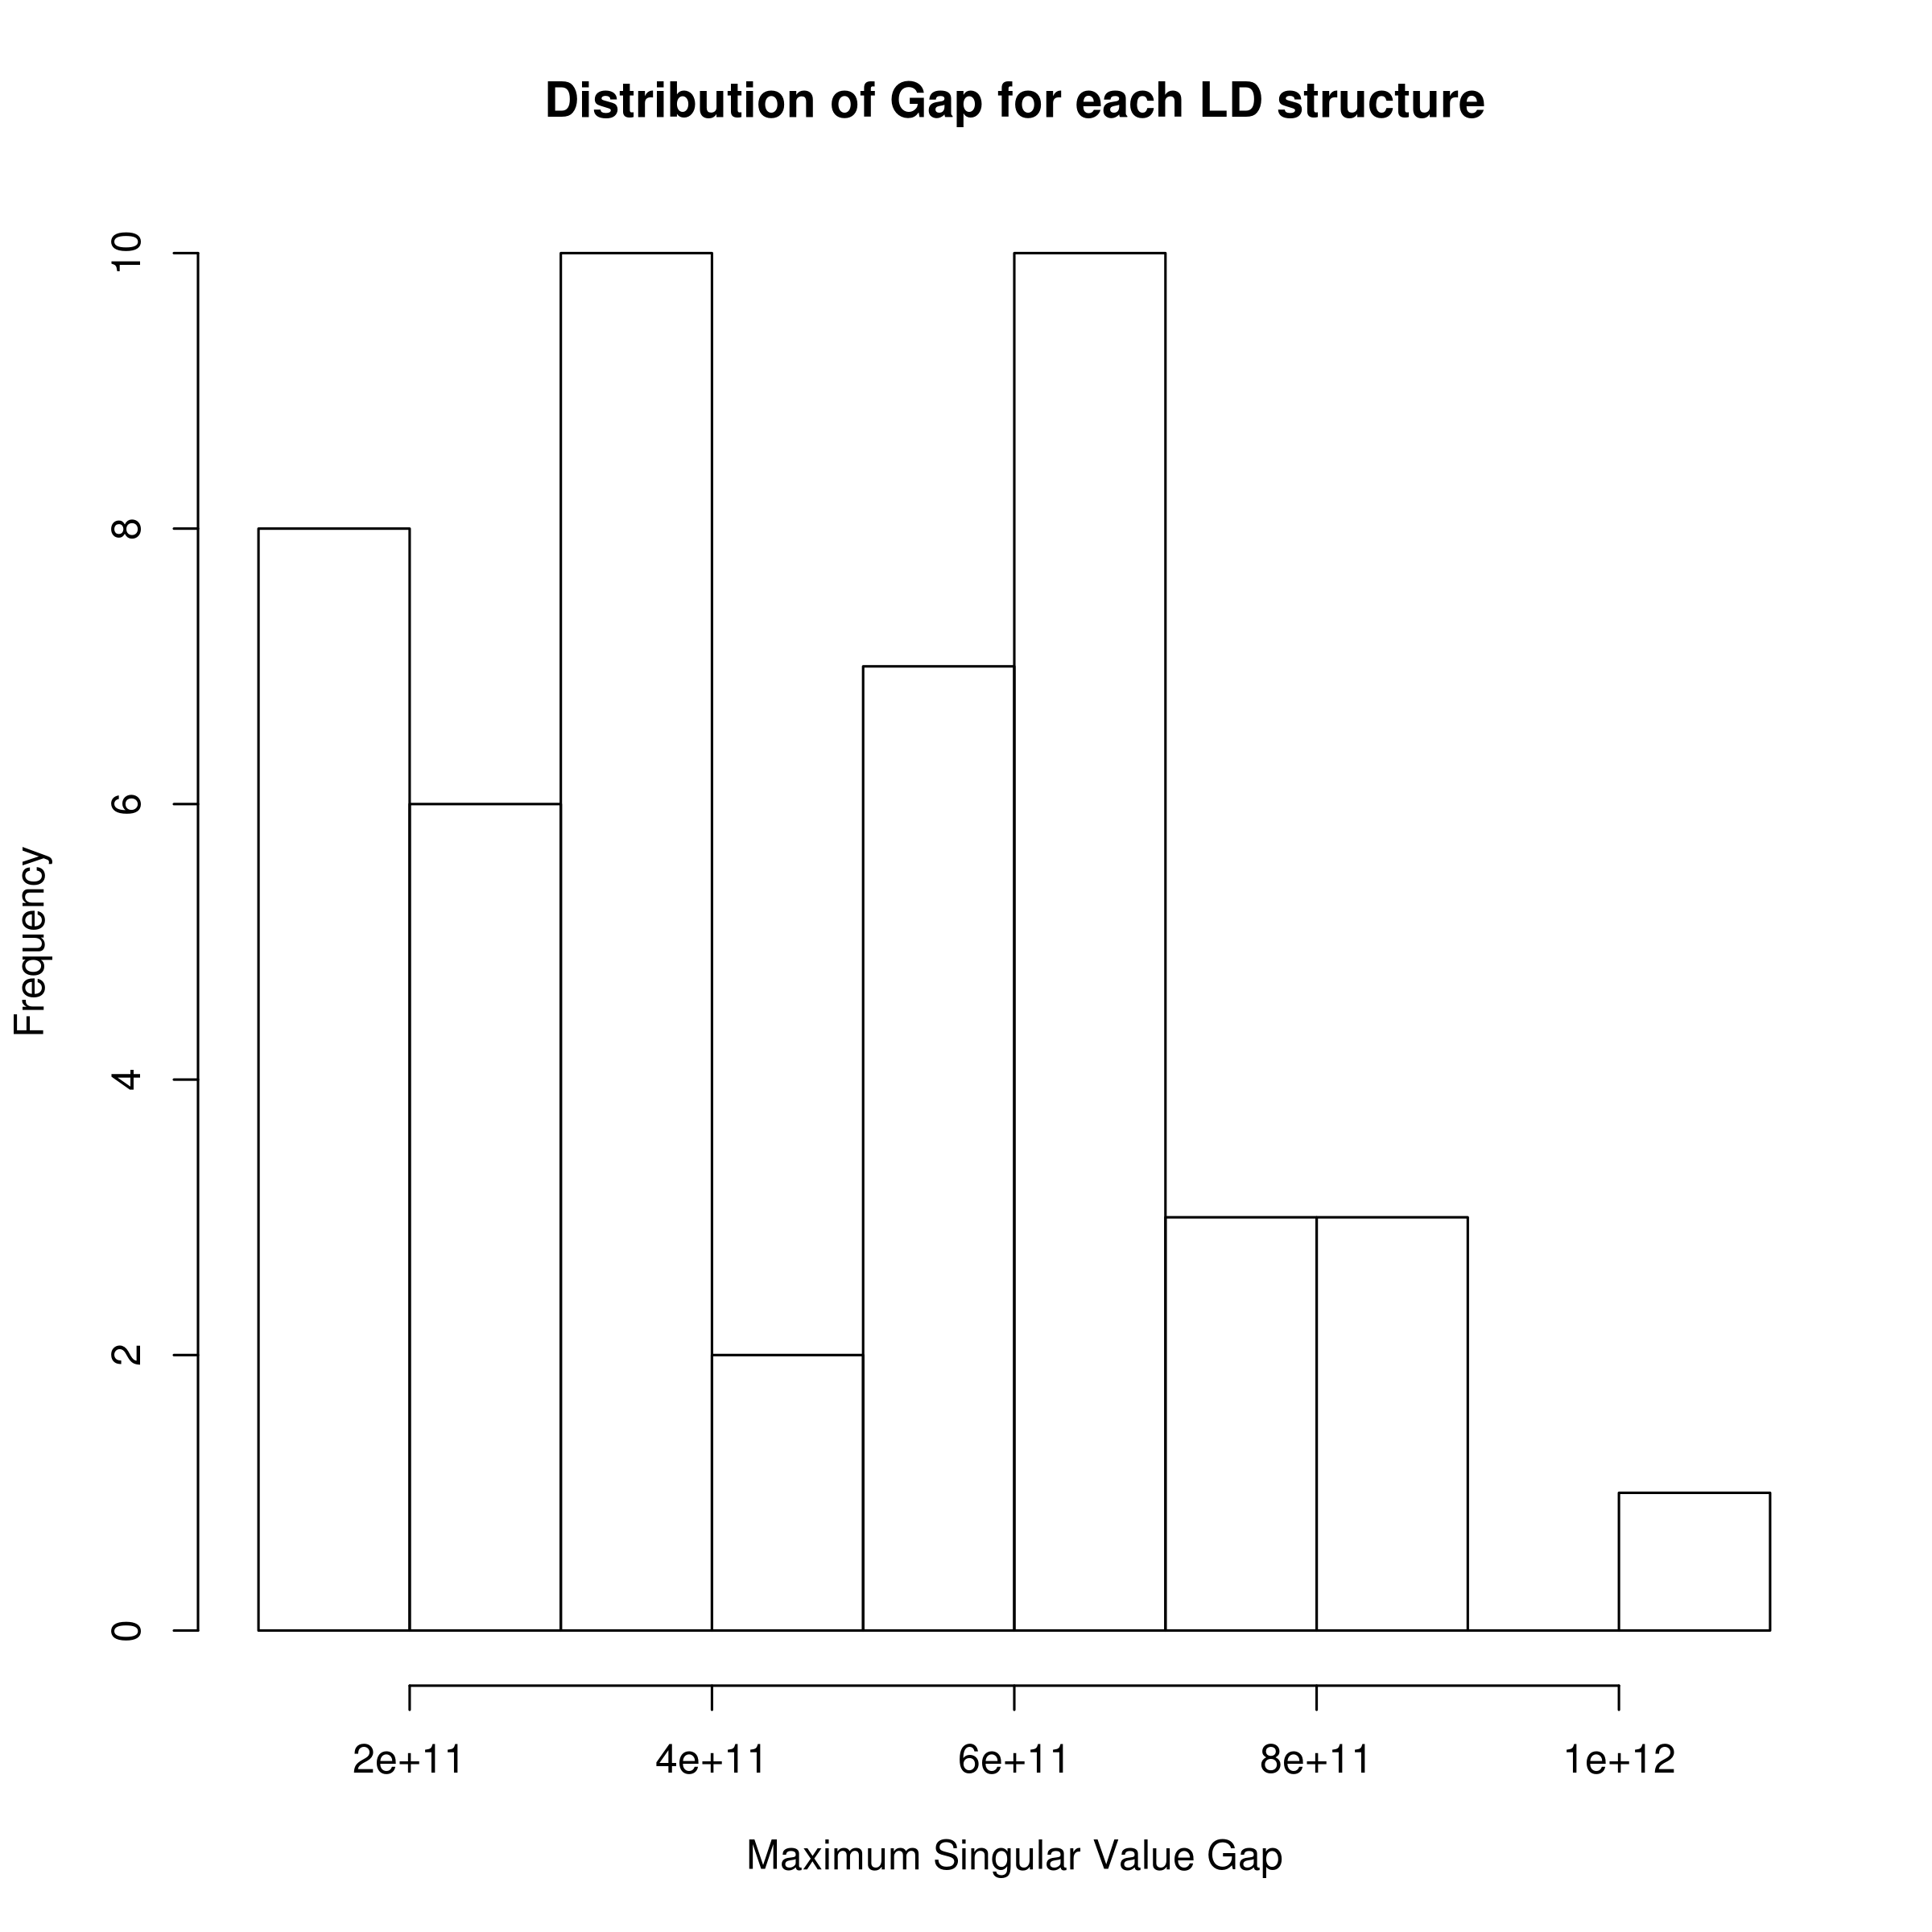
\includegraphics[width=0.5\textwidth]{figure/singular_value_distribution.png}
				\label{fig:singularValueDist}
				\vspace{-20pt}
			\end{figure}
			%\end{wrapfigure}
			
			By employing the \gls{tSVD} as a method for regularization, we were able to solve the ill-posed \cref{eq:shrekEq}, and obtain the estimated heritability.
						
		\subsection{Comparing with \glsentrylong{ldsc}}
	
		
	\section{Simulation}
		We implemented the heritability estimation in \gls{shrek} and in order to assess how well \gls{shrek} performs for heritability estimation in comparison to other current methods, we performed a series of systematic simulations.
		In these simulations, we compared the performance of \gls{shrek} with \gls{gcta}\citep{Yang2011} and the \gls{ldsc}\citep{Bulik-Sullivan2015} with and without the intercept estimation function (-{}-no-intercept). 
		
		Through simulation, we can obtain the sample distribution of the heritability estimate under different study designs (e.g. Quantitativat traits, Case-Control studies or extreme phenotype selection). 
		%We can also evaluate the performance of different methods under varying genetic architecture (e.g. different number of Snps, different LD structures) or even with different disease models (e.g. different number of causal Snps, different heritability).
		
		It was extremely important for us to consider as much possible conditions as possible.
		Here we will outline all the parameters used in the simulation.
		\subsection{Sample Size}
		The sample size was one of the most important parameter in determining the standard error of the heritability estimation. 
		As the sample size increases, study will be more representative of the true population and therefore generate a more stable and accurate results.
		
		Using simple text mining technique, we have calculated the average sample size for all \gls{GWAS} recorded on the \gls{GWAS} catalog\citep{Welter2014} was around 7,200 samples.
		We argue that if all the tools were able to preform well when the sample size was small, then they should have no problem handling larger data sets.
		Thus, we only simulate 1,000 samples in our simulation and if all the tools can accurately estimate the heritability, then they should have no problem in estimating the heritability when there were more samples.
		
		\subsection{Number of SNPs in Simulation}
		As technology progress, the number of \glspl{SNP} on each array chip has increased significantly.
		We can now achieve a single base pair resolution using the \gls{ngs} technologies.
		However, it was computationally infeasible for us to simulate a large amount of \glspl{SNP} in every single simulation. 
		Considering that one can usually partition the whole genome into individual chromosomes during the heritability estimation, we therefore only simulate chromosome 1 with 50,000 \glspl{SNP} in majority of the simulations.
		
		\subsection{Genetic Architecture} % Should contain the effect size distribution, the causal SNP number and the heritability spectrum
		
		\subsection{Case Control Studies}
		\subsection{Extreme Phenotype Selection}
		\subsection{Quantitative Trait}
		
			One important factor to consider when carrying out a simulation is that the result of the simulation should be translatable to real life situation. 
			Therefore, it is vital for us to consider as many different scenario as possible.
			When simulating a quantitative trait, there are a number of parameter for one to consider, for example, the sample size, the number of \glspl{SNP}, the number of causal \glspl{SNP} and the true heritability of the trait are all important parameters. 
			However, it is also unrealistic for one to test the combination of all of these parameter as that will require a large amount of processing time. 
			Thus, we aim to strike a balance between comprehensive test case and a realistic simulation time. 
			
			First, although the average samples size for all current \gls{GWAS} was $\sim$ 7,200 samples based on \gls{GWAS} in the \gls{GWAS} Catalog\citep{Welter2014}, we only used 1,000 samples in our simulation.
			We argue that if the tools were able to perform well when a small sample size were provided, then they should perform equally, if not better, when a larger sample size is given. 
			
			Secondly, we tried to simulate the complex \gls{LD} structure in human population.
			Therefore, we used HAPGEN2\citep{Su2011} with the 1000 genome \gls{CEU} population structure as an input to simulate samples with \gls{LD} structure comparable to that in the 1000 genome \gls{CEU} samples.
			Considering that it is unlikely for any \glspl{SNP} between two chromosome to be in \gls{LD}, we limit our simulation to chromosome 1 where there are a total of 670,052 \glspl{SNP} information available for use in simulation.
			However, it was noted that as number of \glspl{SNP} increase, the time required for simulating the samples and sample phenotype become prohibitive high. 
			As a result of that, we limit the number of \glspl{SNP} simulated to 50,000. 
			
			Trait complexity and trait heritability usually dictates the performance of heritability estimation.
			For example, if the trait is a Mendelian trait where there is a single causal \gls{SNP} with large effect size, it will be relatively easy to calculate the trait's heritability.
			However, when a trait is polygenic with large amount of causal \glspl{SNP}, each contribute a small portion of effect (e.g. \gls{scz}), it will be challenging to estimate the heritability.
			We therefore varies the number of causal \glspl{SNP} $k$ with $k\in\{10,50,100,1000\}$ such that different spectrum of trait complexity (e.g. oligogenic to polygenic) will be tested. 
			One exception was Mendelian traits where we omitted from our simulation.
			It was because Mendelian traits usually associate with a single rare \gls{SNP} with large effect size and high penetrance where its heritability can easily be estimated without the use of such complex algorithms.
			
			Besides trait complexity, the trait heritability also dictates the performance of heritability estimation. 
			We would therefore simulate traits with heritability $H$ where $H\in[0,1)$. 
			Based on the work of \citet{Orr1998}, we modeled our per-\gls{SNP} effect size to follow an exponential distribution with $\lambda=1$, which serves as a heuristic expectation of the genetic architecture of adaptation.
			Taken into account of the number of causal \glspl{SNP} and target heritability $H$, we then calculate the per-\gls{SNP} effect size as
			\begin{align}
			\beta_i &\sim exp(1)\notag\\
			\boldsymbol{\beta}&=(\beta_1,\beta_2,...,\beta_k)^t\notag\\
			\boldsymbol{\gamma} &= \frac{H}{k}\boldsymbol{\beta}
			\label{eq:snpEffect}
			\end{align}
			where $\boldsymbol{\gamma}$ is the vector of per SNP effect size and $H$ is the simulated heritability.
			The final heritability of the simulated trait is defined as $H_{final}=\boldsymbol{1}^t\boldsymbol{\gamma}$
			
			Another consideration is the \gls{SNP} \gls{maf}, which tends to correlate with effect size\citep{Manolio2009} due to selection.
			Rare \glspl{SNP} with a small \gls{maf} tend to have a large effect size whereas common \glspl{SNP} tend to have a small effect size. 
			Therefore, after the per \gls{SNP} effects were simulated, we distribute the effect size to $k$ randomly selected \gls{SNP}(s) according to their \gls{maf}.
		
			Finally, by assuming $\boldsymbol{X}$ to be the standardized genotype of $k$ causal SNPs in $n$ samples, one can get the phenotype of the simulated samples based on \cref{eq:snpEffect} using
			\begin{align}
			\epsilon_i&\sim N(0,\sqrt{\mathrm{Var}(\boldsymbol{X\gamma})\frac{1-H_{final}}{H_{final}}} )\notag\\
			\boldsymbol{\epsilon} &= (\epsilon_1,\epsilon_2,...,\epsilon_n)^t\notag\\
			\boldsymbol{y} &= \boldsymbol{X\gamma}+\boldsymbol{\epsilon}
			\label{eq:simulationOfPhenotype}
			\end{align}
			
			For each batch of simulated samples, we calculate the estimated heritability using \gls{shrek}, \gls{gcta}, \gls{ldsc} with intercept fixed at 1 and \gls{ldsc} allowing for intercept estimation for each $H$.
			In each iteration, the sample genotype was provided to \gls{gcta} for the calculation of genetic relationship matrix (GRM) whereas for \gls{shrek} and \gls{ldsc} 500 additional samples were simulated based on the 1000 genome project \gls{CEU} samples\parencite{Project2012} to construct the \gls{LD} matrix and calculate the \gls{LD} score respectively. 
			This is because in general situations, \gls{ldsc} and \gls{shrek} will not be provide with the sample genotype, instead, these programmes were designed to work with external \gls{LD} reference data.
			Therefore to provide a realistic simulation, an independent set of reference samples were provided for \gls{shrek} and \gls{ldsc}.
			  
			The whole process were repeated 50 times to obtain the empirical variance of the estimates,.
			In each iteration, new set of samples were simulated with the \glspl{SNP} set, the causal \glspl{SNP} and the per \gls{SNP} effect size remain unchanged for each $H$.
			%In order to determine a realistic and reasonable sample size for all simulation condition, we manually curated the sample size of all the studies presented on the \gls{GWAS} Catalog\cite{Welter2014} (version 2015-07-17) to get the distribution of sample size in existing studies.
			%It was observed that the mean sample size of all published \gls{GWAS} is $\sim$ 7,200 samples. 
			%Thus, we consider a simulation sample size of 7,200 should be comparable to general \gls{GWAS} studies.
			%Although a large sample size are generally required for \gls{GWAS}, it might also worthwhile for one to test the performance when only small sample size is available.
			%If the tools perform well with a small sample size, it will be beneficial to studies of rare complex traits where it is often difficult to collect a large amount of samples.
			%As a result of that, we also perform simulation with 1,000 samples.
			
			To summarize, 
			\begin{enumerate}
				\item Randomly select 50,000 \glspl{SNP} from chromosome 1
				\item Randomly generate $k$ effect size following \cref{eq:snpEffect} where $k \in \{10,50,100,1000\}$
				\item Randomly assign the effect size to $k$ \glspl{SNP} where \glspl{SNP} with small \gls{maf} will get a large effect size.
				\item Simulate 1,000 samples using HAPGEN2 and calculate their phenotype according to \cref{eq:simulationOfPhenotype}
				\item Perform heritability estimation using \gls{shrek}, \gls{ldsc} and  \gls{gcta}
				\item Repeat step 4-5 50 times
				\item Repeat step 1-6 50 times
			\end{enumerate}
			
			
		\subsection{Case Control Studies}
		Similar to quantitative trait simulation, the sample size, the number of \glspl{SNP}, the number of causal \glspl{SNP} and the true heritability of the trait are important parameters to consider during simulation. 
		On top of that, there are a few more parameters one must consider during the simulation of case control studies such as the population prevalence of the trait and the observed prevalence of the study. 
		
		To simulate cases and controls, we will need to simulate the liability distribution by taking into acount of the prevalence. 
		So for example, if one like to simulate a trait with population prevalence of $p$ and observed prevalence  of $q$ and would like to have $n$ cases in total, one will have to simulate $\min(\frac{n+pn}{p}, \frac{n+qn}{q})$ samples.
		It is therefore challenging for one to simulate scenario with a small $p$ or $q$ values. 
		
		In this study, we fixed $q=0.5$ and varies $p\in\{0.5,0.1\}$. Although disease such as \gls{scz} can have a prevalence $\approx1\%$, the required sample numbers become infeasible for large scale simulation where a minimum of 101,000 samples will be required if we wish to obtain 1,000 cases.
		Despite our wish to simulate conditions with small prevalence, the limitation of computation power simply forbade us to undergo such simulation. 
		
		Once the liability distribution were simulated, cases can be drawn from samples with a liability higher than the liability threshold. 
		The liability threshold was calculated as the value $> 1-p$ of all values under the standard normal distribution using the \emph{qnorm} function in R. 
		Samples with a liability lower than the liability threshold were then considered as control samples. 
		1,000 cases and 1,000 controls were then randomly drawn from the corresponding population of samples.
		 
		To summarize, 
		\begin{enumerate}
			\item Randomly select 50,000 \glspl{SNP} from chromosome 1
			\item Randomly generate $k$ effect size following \cref{eq:snpEffect} where $k \in \{10,50,100,1000\}$
			\item Randomly assign the effect size to $k$ \glspl{SNP} where \glspl{SNP} with small \gls{maf} will get a large effect size.
			\item Simulate $\frac{n+qn}{q}$ samples using HAPGEN2 where $q\in\{0.5,0.1\}$
			\item Simulate sample phenotype according to the liability threshold where 1,000 cases and 1,000 controls were obtained
			\item Perform heritability estimation using \gls{shrek}, \gls{ldsc} and  \gls{gcta}
			\item Repeat step 4-6 50 times
			\item Repeat step 1-7 50 times
		\end{enumerate}
		
		\subsection{Exreme Phenotype Selections}
		The simulation of extreme phenotype selection is very much like the combination of quantitative trait simulation. 
		The simplest way to simulate the extreme phenotype selection is to first simulation $N$ samples, then from this population of samples, select $n$ samples from both end of the population and use them to perform association and heritability estimation.
		
		Due to the similarity in nature with the simulation of quantitative traits and case control studies, we limit the number of causal \glspl{SNP} simulated as 100. 
		We also limit our simulation to select samples with phenotype on the top and bottom $10\%$ of the population.
		
		However, it was noted that both \gls{gcta} and \gls{ldsc} did not implement heritability estimation under extreme phenotype selection. 
		To perform a fair comparison with \gls{shrek}, we calculate the adjustment factor $\frac{\mathrm{Var}(Phenotype\ before\ selection)}{\mathrm{Var}(Phenotype\ after\ selection)}$ to the estimation from \gls{gcta} and \gls{ldsc}.
		
		Therefore, to summarize,
		\begin{enumerate}
			\item Randomly select 50,000 \glspl{SNP} from chromosome 1
			\item Randomly generate 100 effect size following \cref{eq:snpEffect}
			\item Randomly assign the effect size to $k$ \glspl{SNP} where \glspl{SNP} with small \gls{maf} will get a large effect size.
			\item Simulate 10,000 samples using HAPGEN2 and calculate their phenotype according to \cref{eq:simulationOfPhenotype}
			\item Select the top and bottom $10\%$ of samples from the 10,000 samples.
			\item Perform heritability estimation using \gls{shrek}, \gls{ldsc} and  \gls{gcta}
			\item Manually apply the adjustment factor to estimation of \gls{gcta} and \gls{ldsc}
			\item Repeat step 4-7 50 times
			\item Repeat step 1-8 50 times
		\end{enumerate}
		
	\section{Result}
		The heritabilibty estimation were implemented in \gls{shrek} and is available on \url{https://github.com/choishingwan/shrek}.  
		% We need to find a way to explain our results in a logical sense
		
		\begin{figure}
			\centering
			\centering
			\subfloat[SHREK]{
				\scalebox{.4}{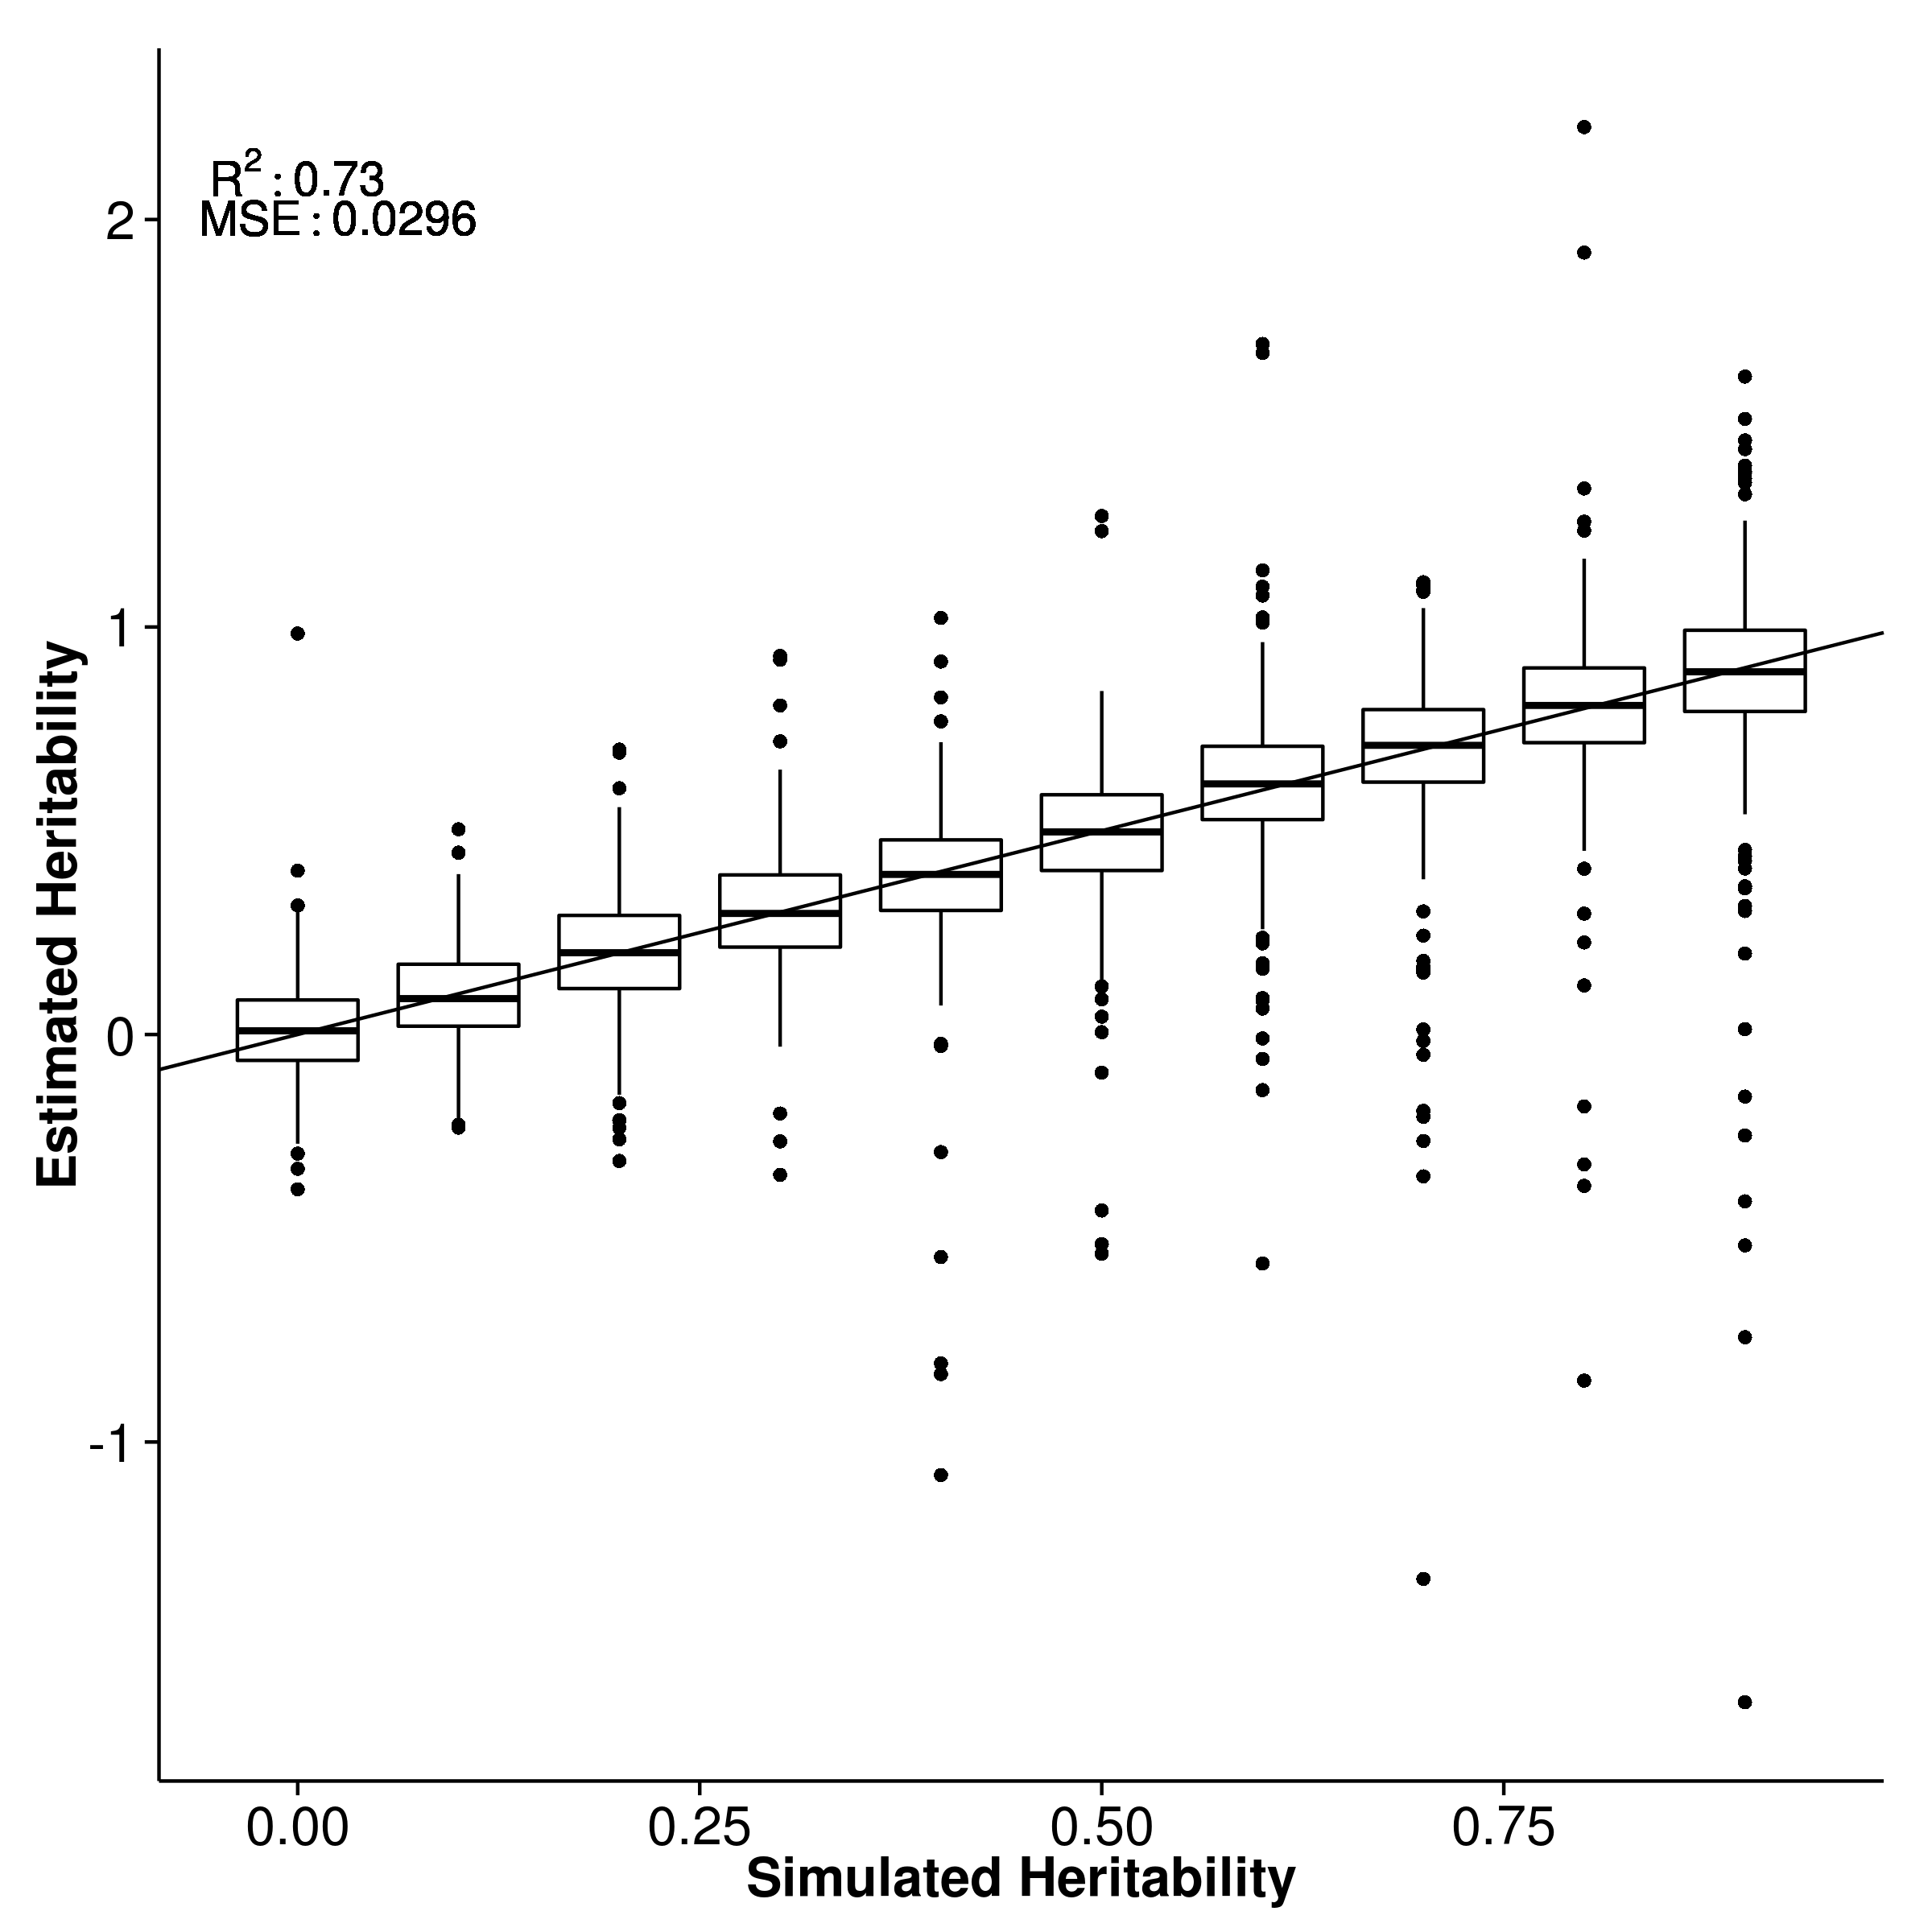
\includegraphics{figure/quantitative/same_effect/10c/shrek_50k_10c_meanH.png}}
				\label{fig:50k10cQtmeanS}
			}
			\subfloat[GCTA]{
				\scalebox{.4}{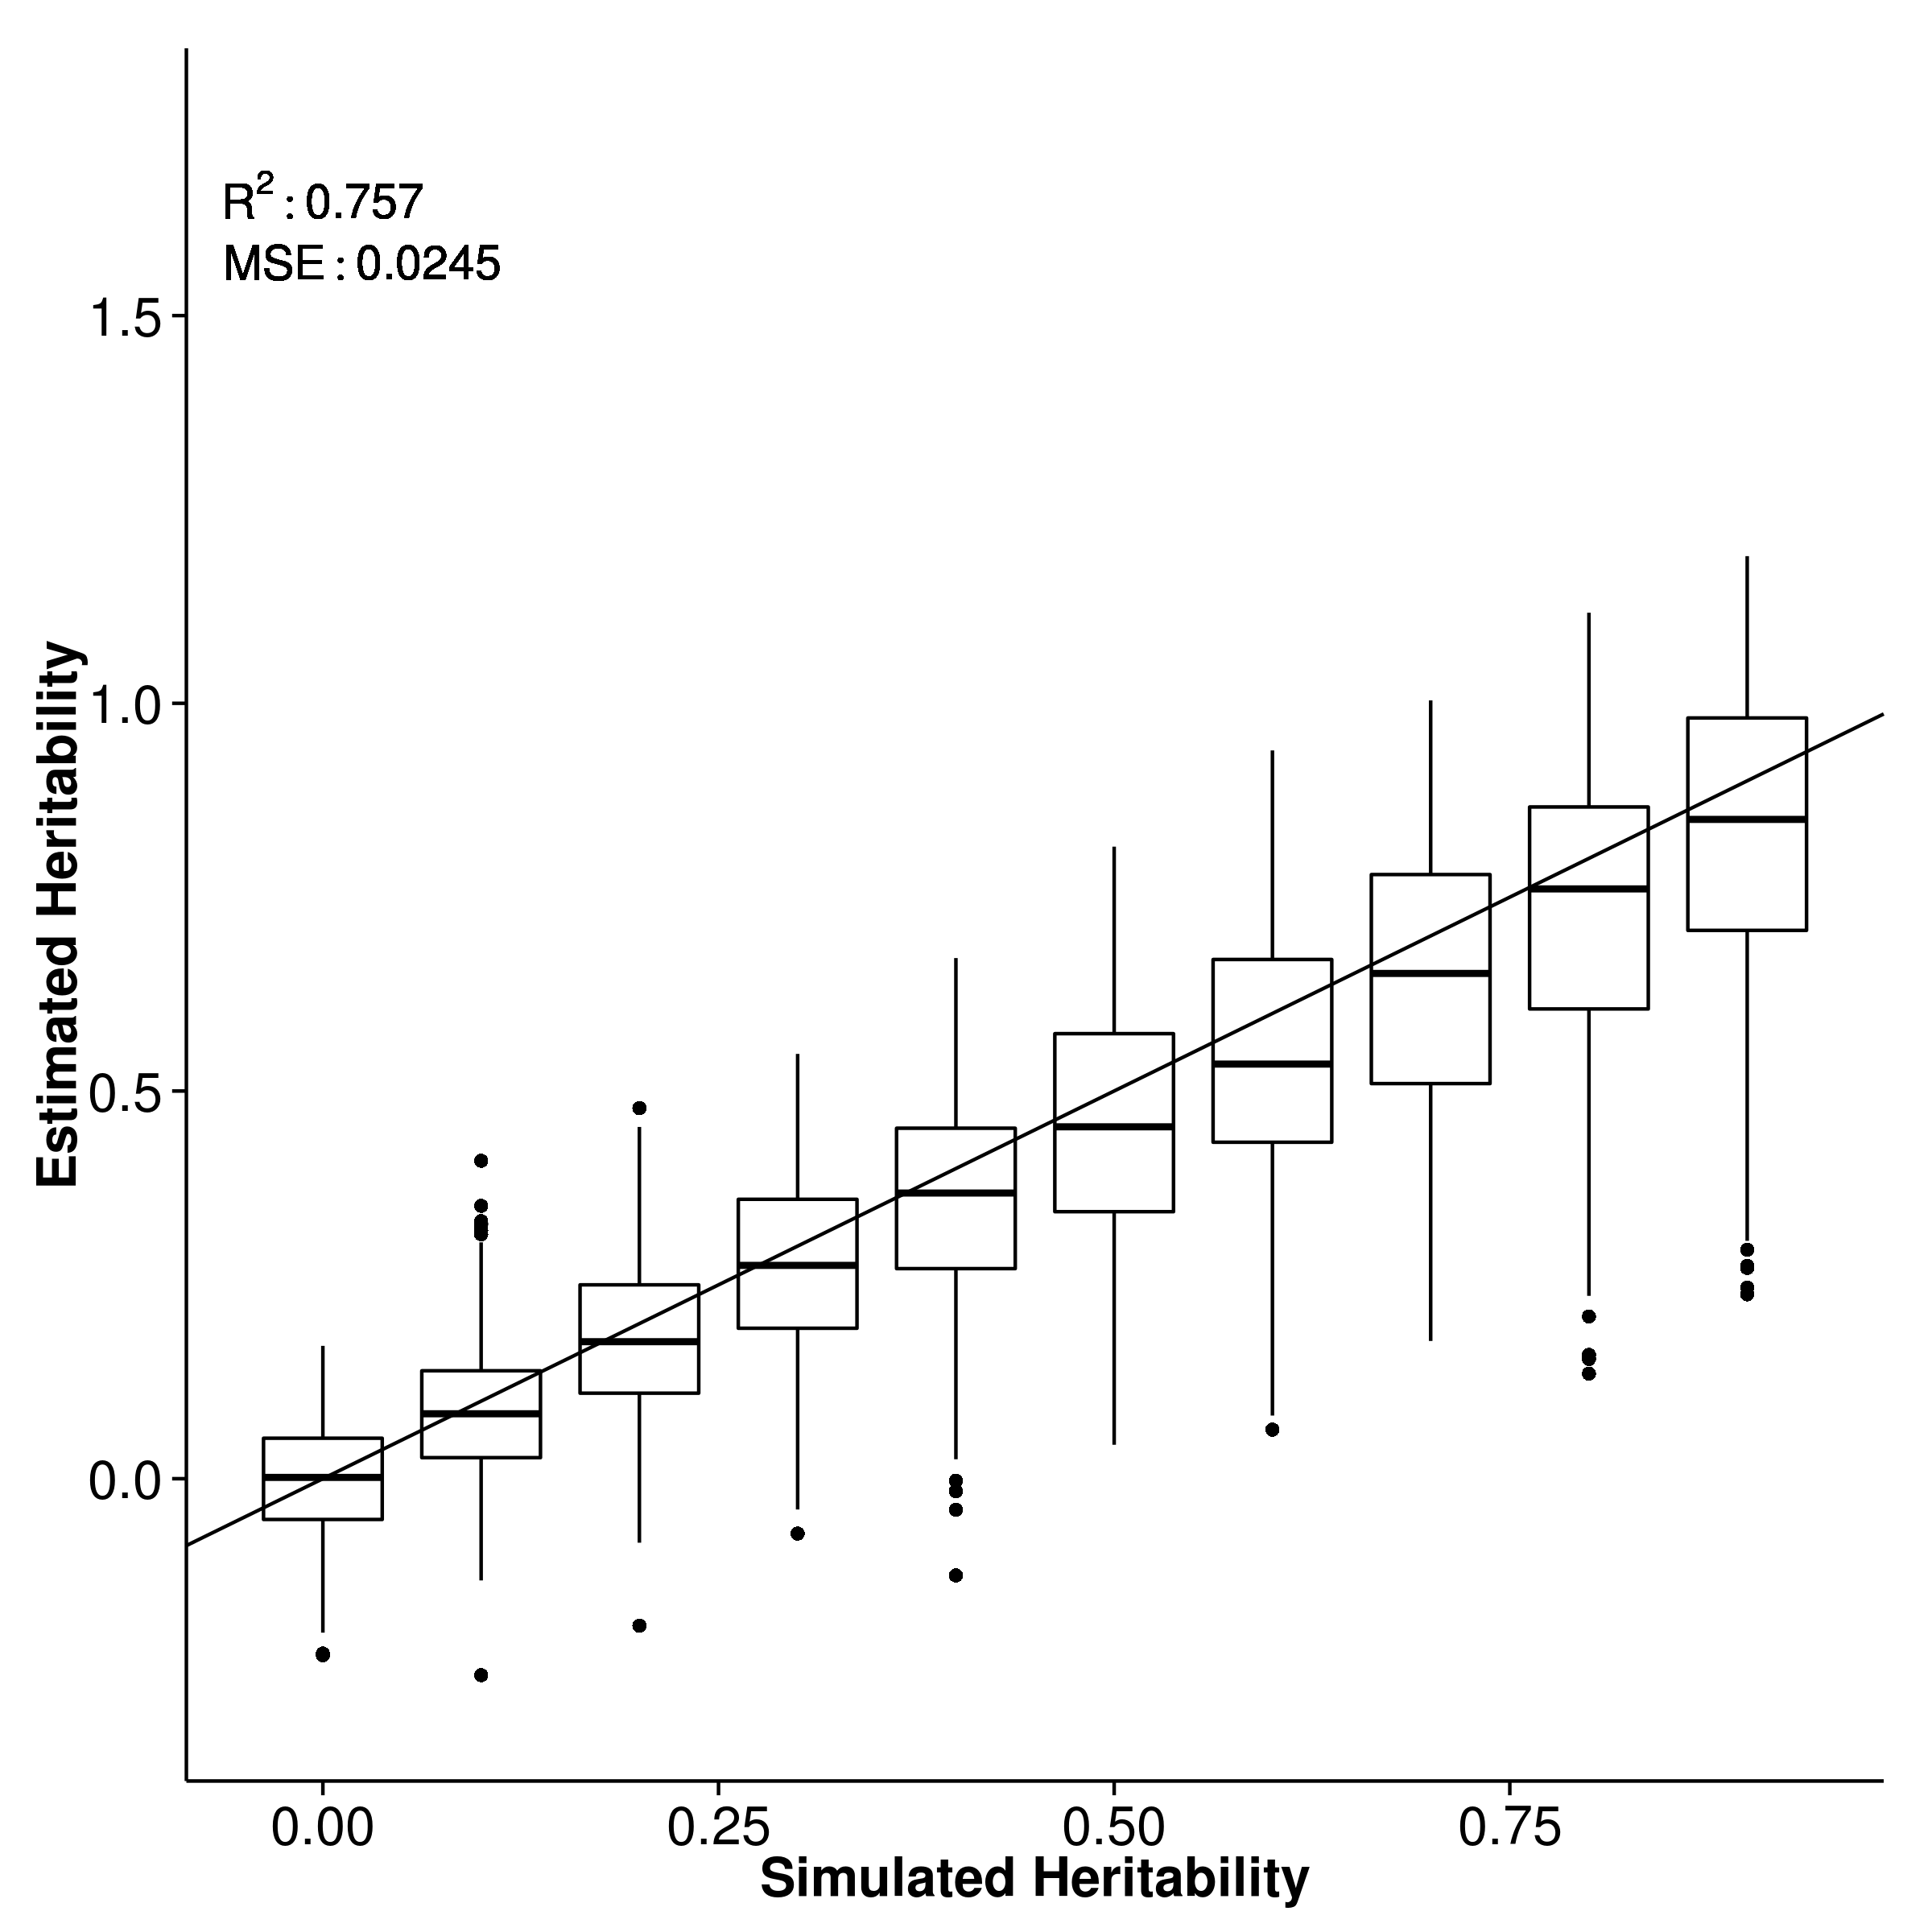
\includegraphics{figure/quantitative/same_effect/10c/gcta_50k_10c_meanH.png}}
				\label{fig:50k10cQtmeanG}
			}\\
			\subfloat[LDSC with fix intercept]{
				\scalebox{.4}{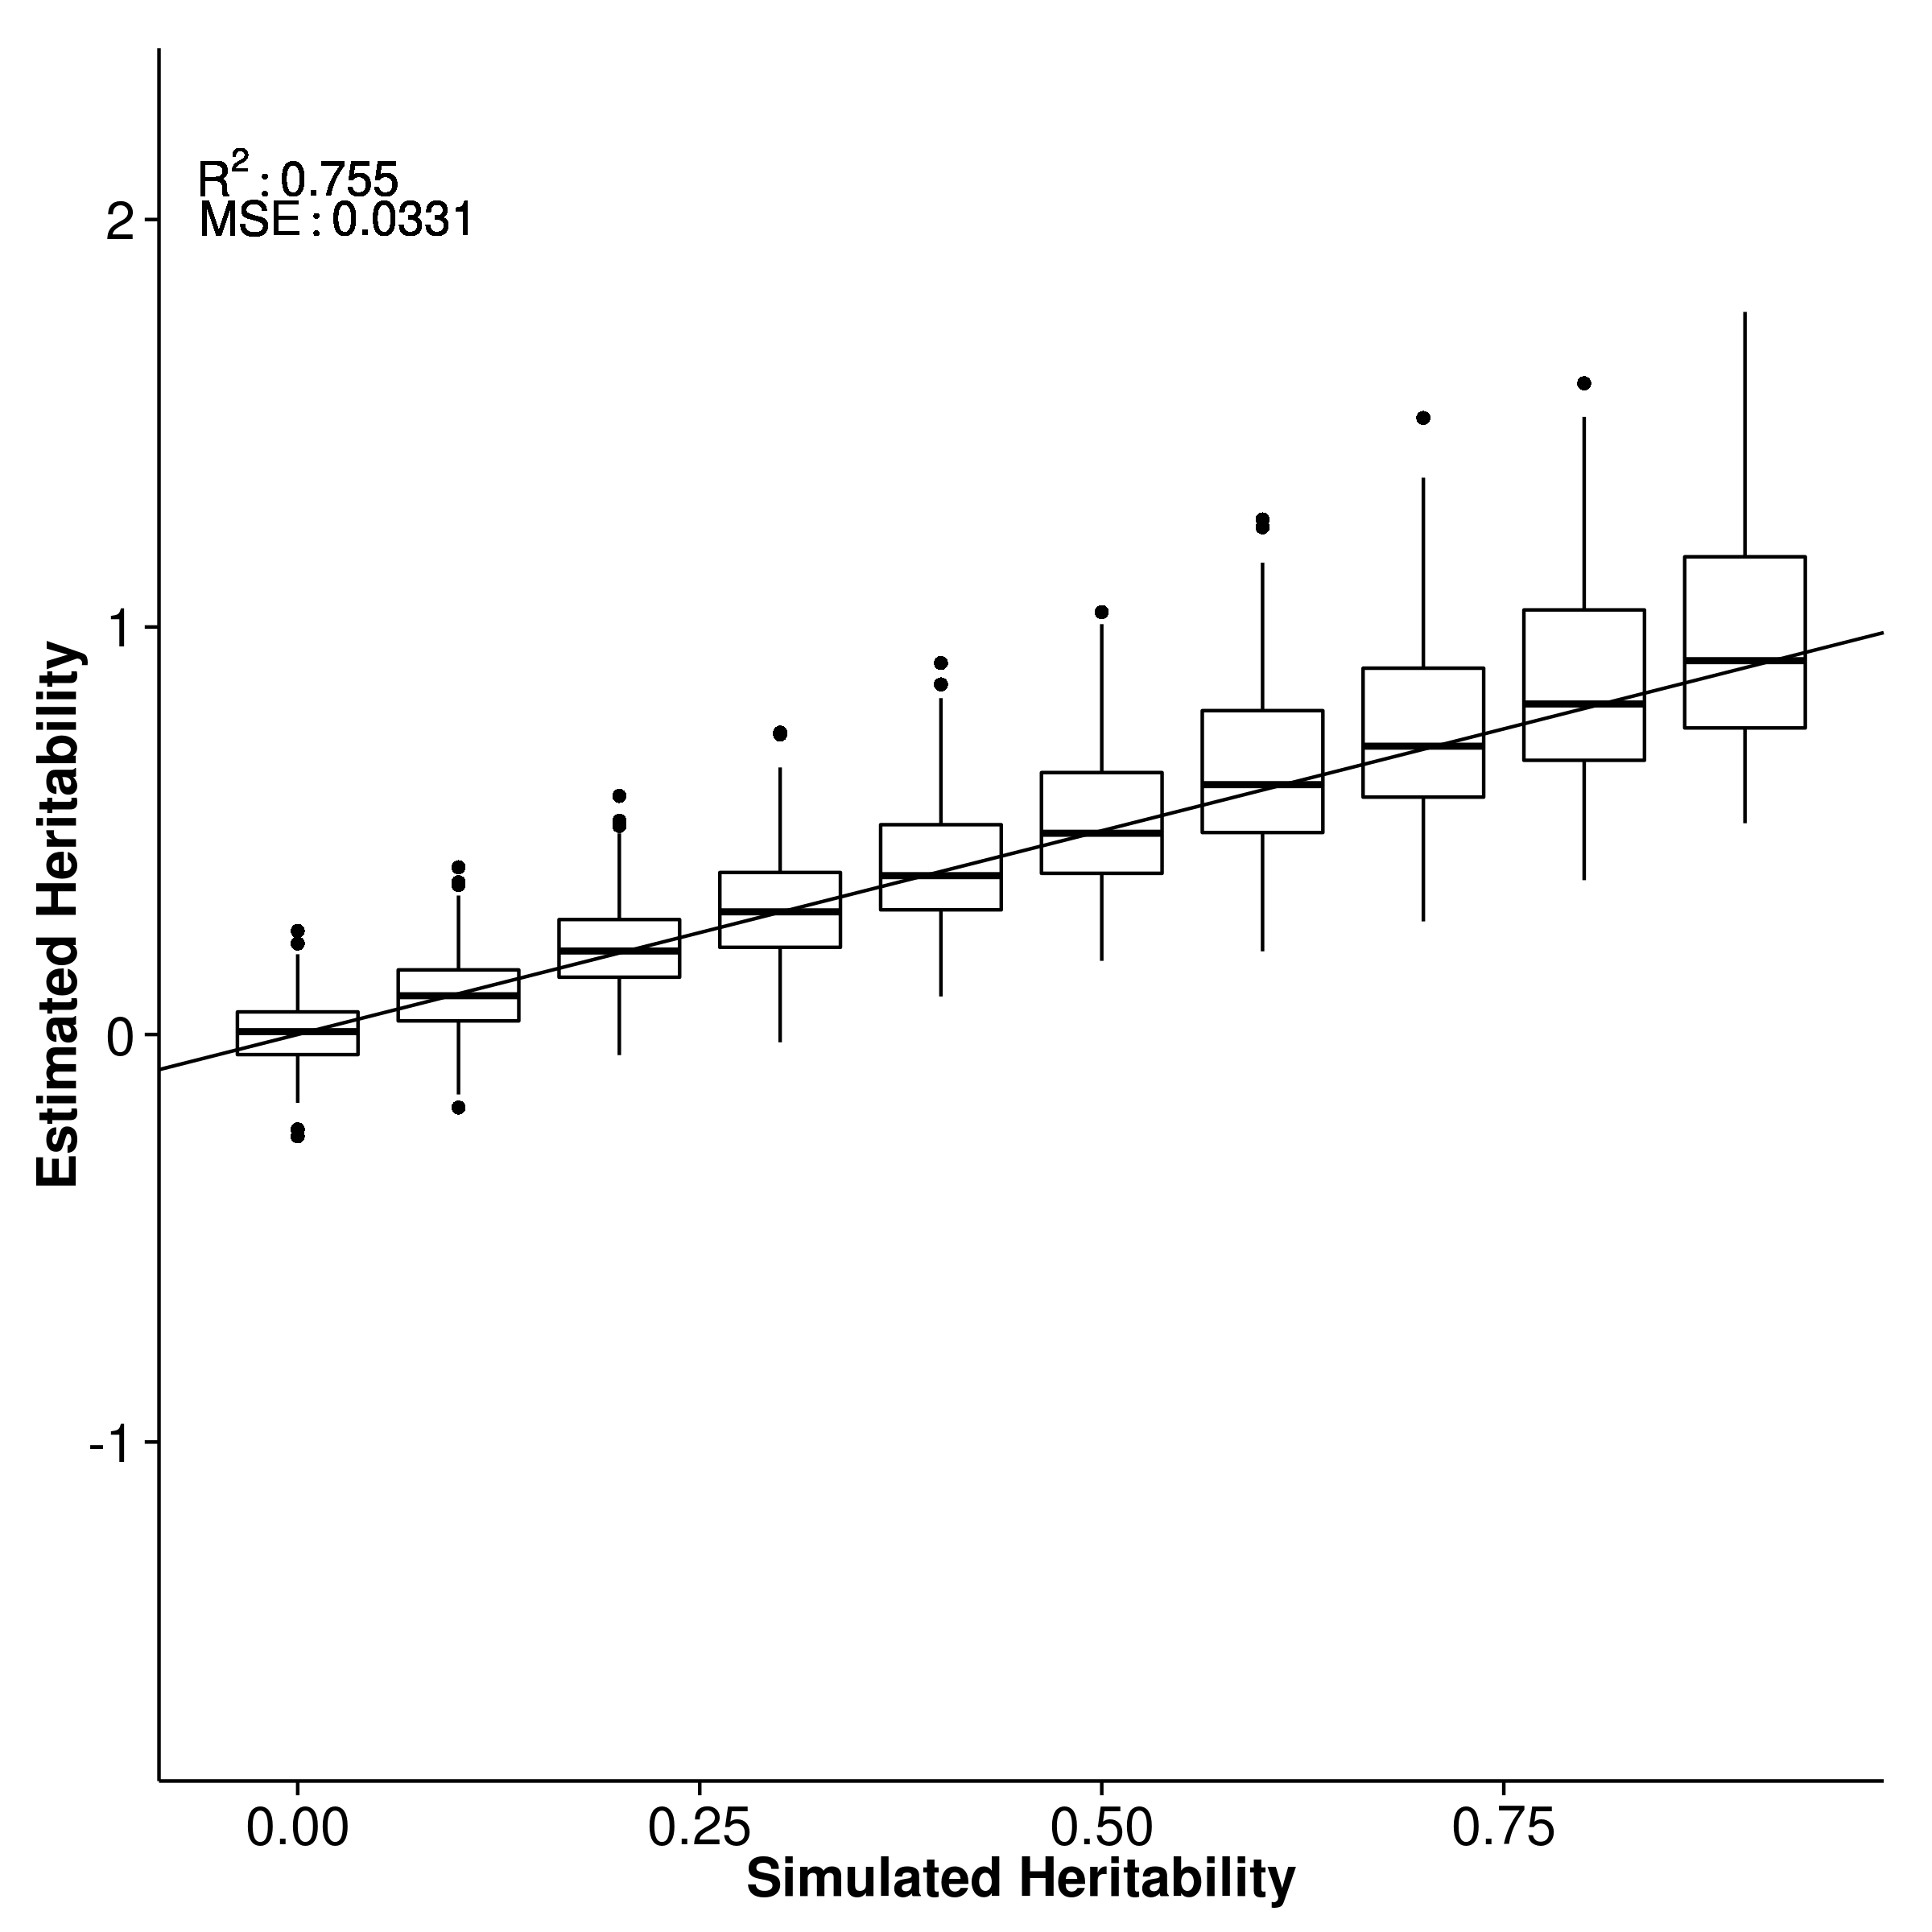
\includegraphics{figure/quantitative/same_effect/10c/ldsc_50k_10c_meanH.png}}
				\label{fig:50k10cQtmeanL}
			}
			\subfloat[LDSC with intercept estimation]{
				\scalebox{.4}{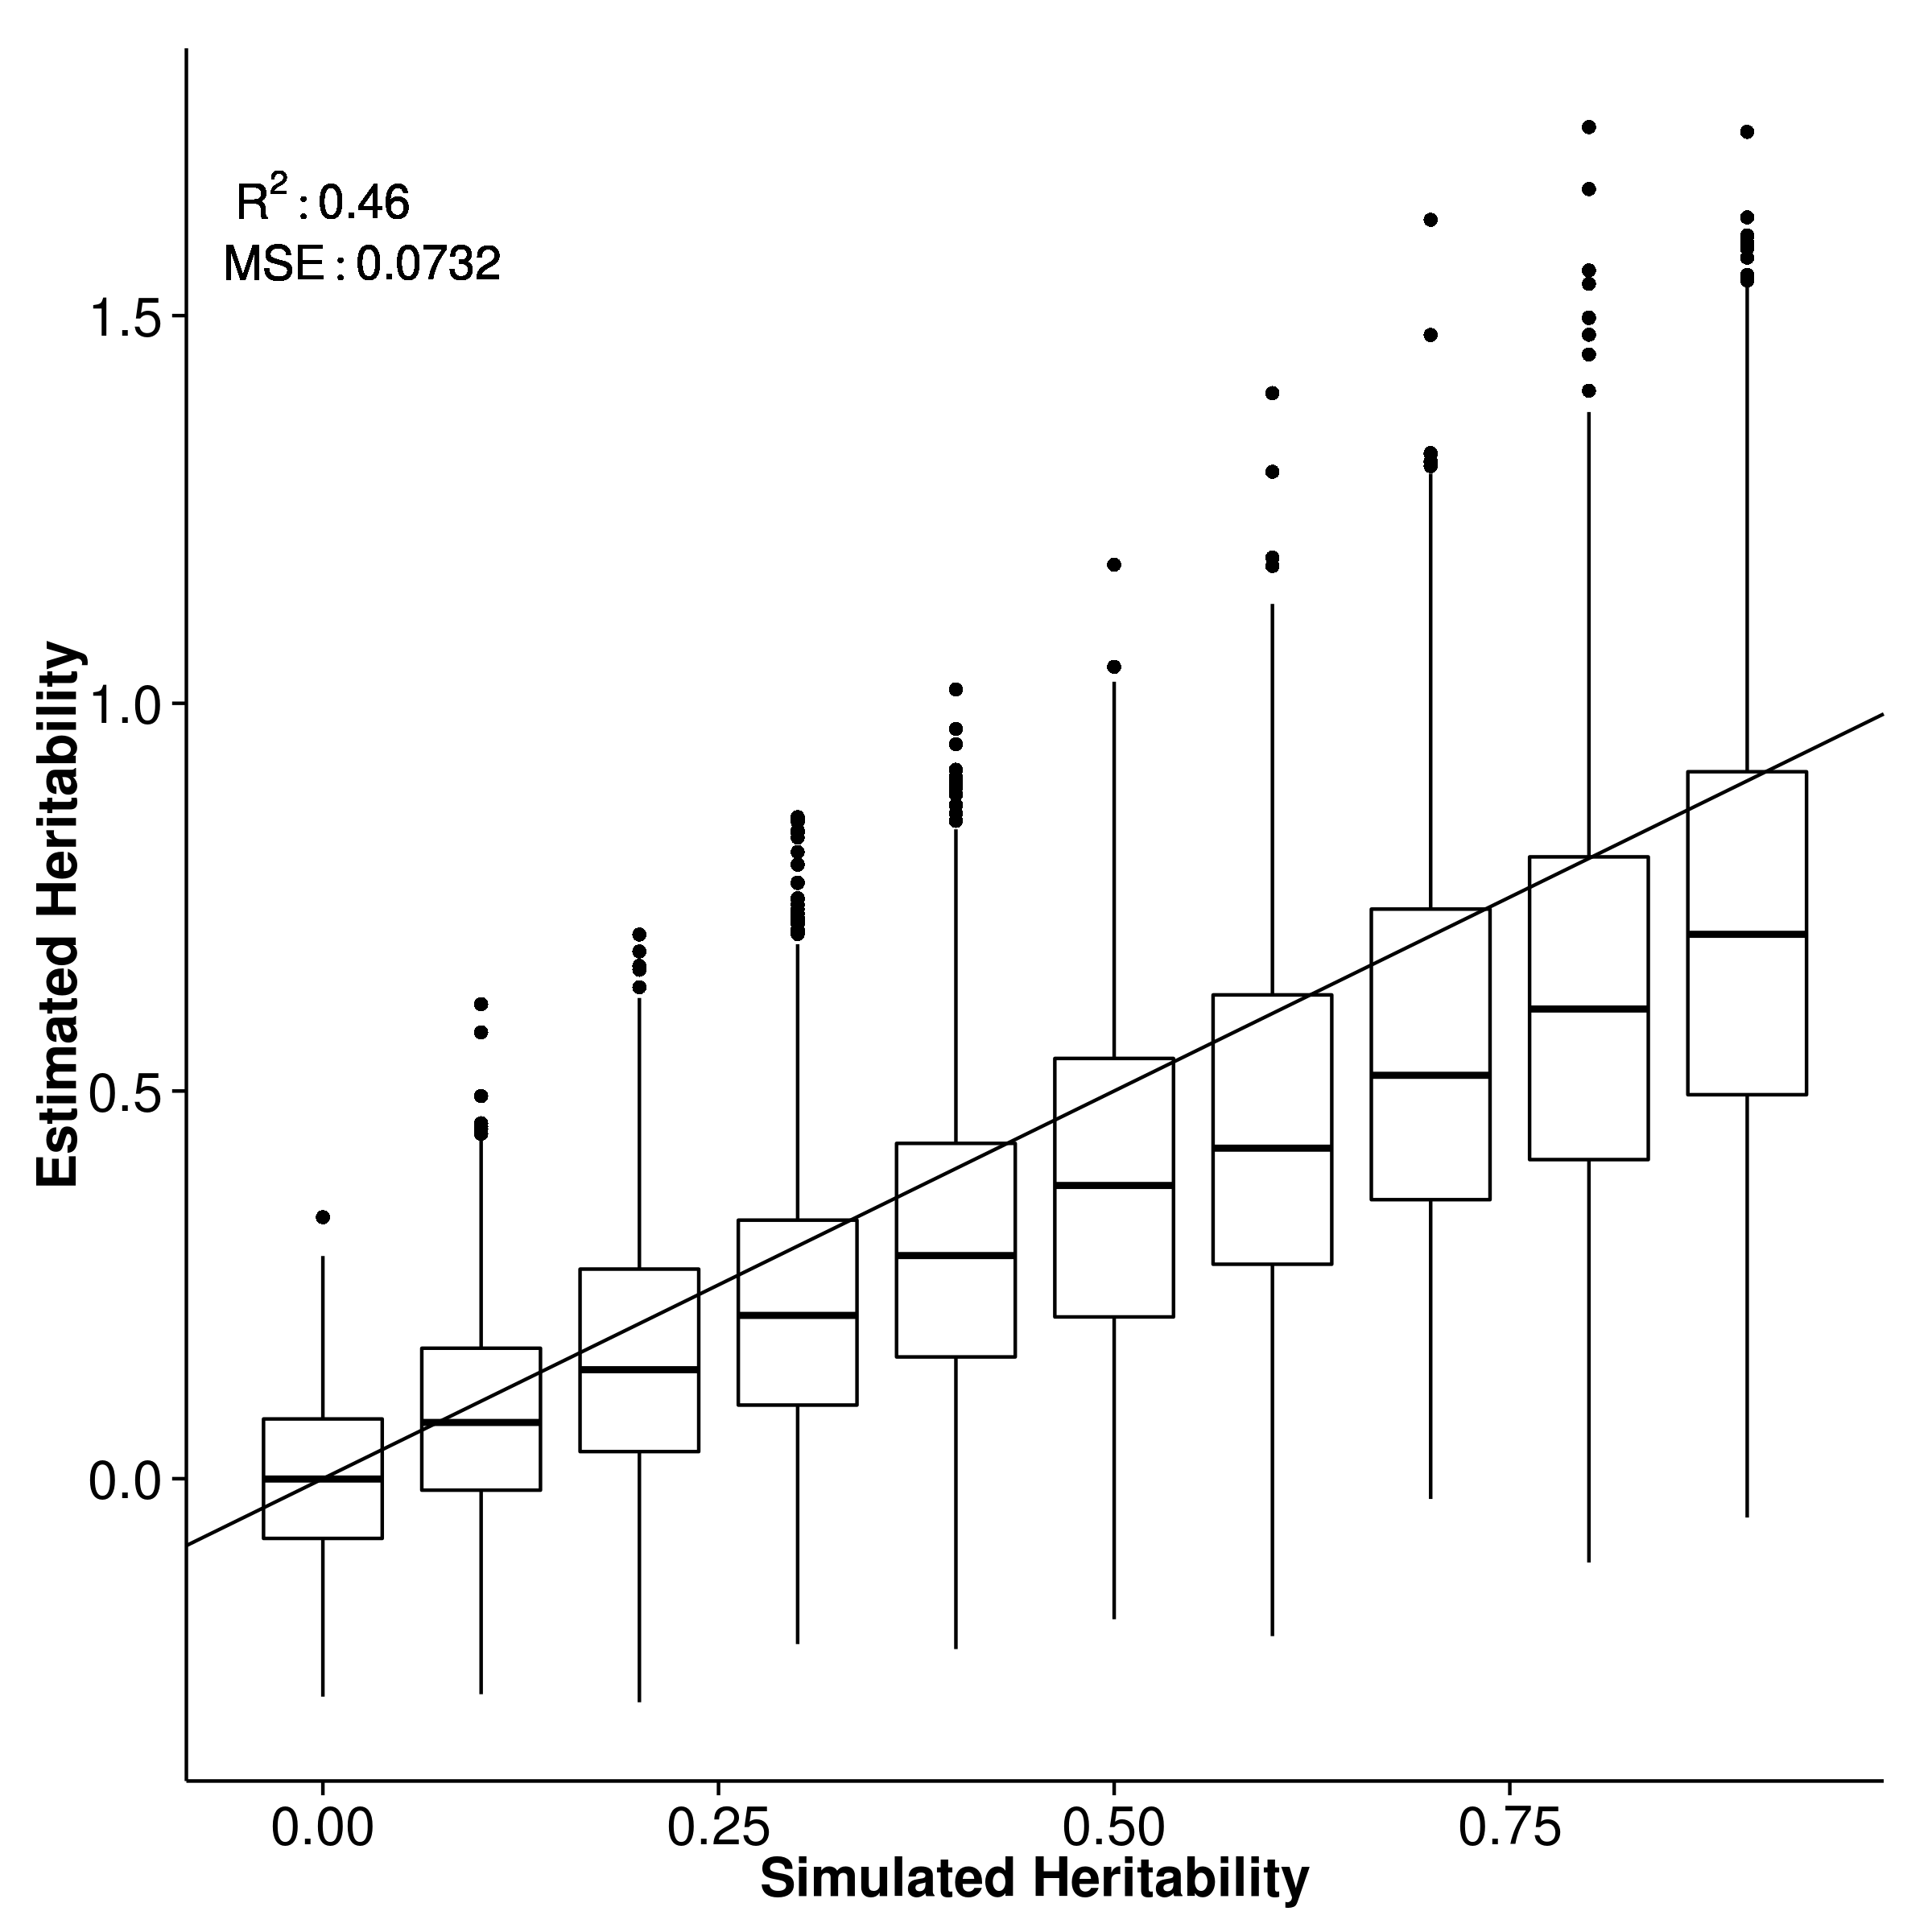
\includegraphics{figure/quantitative/same_effect/10c/ldscIn_50k_10c_meanH.png}}
				\label{fig:50k10cQtmeanI}
			}
			\caption[Simulation of Quantitative Traits with 50k \glsentryshortpl{SNP} and 10 causal variants of same effect size]
			{Simulation of Quantitative Traits with 50k \glsentryshortpl{SNP} and 10 causal variants with same effect size.
				It was observed that of all the tools, \gls{shrek} performed best in such scenario} 
			\label{fig:50k10cQtMean}
		\end{figure}
		\begin{figure}
			\centering
			\centering
			\subfloat[SHREK]{
				\scalebox{.4}{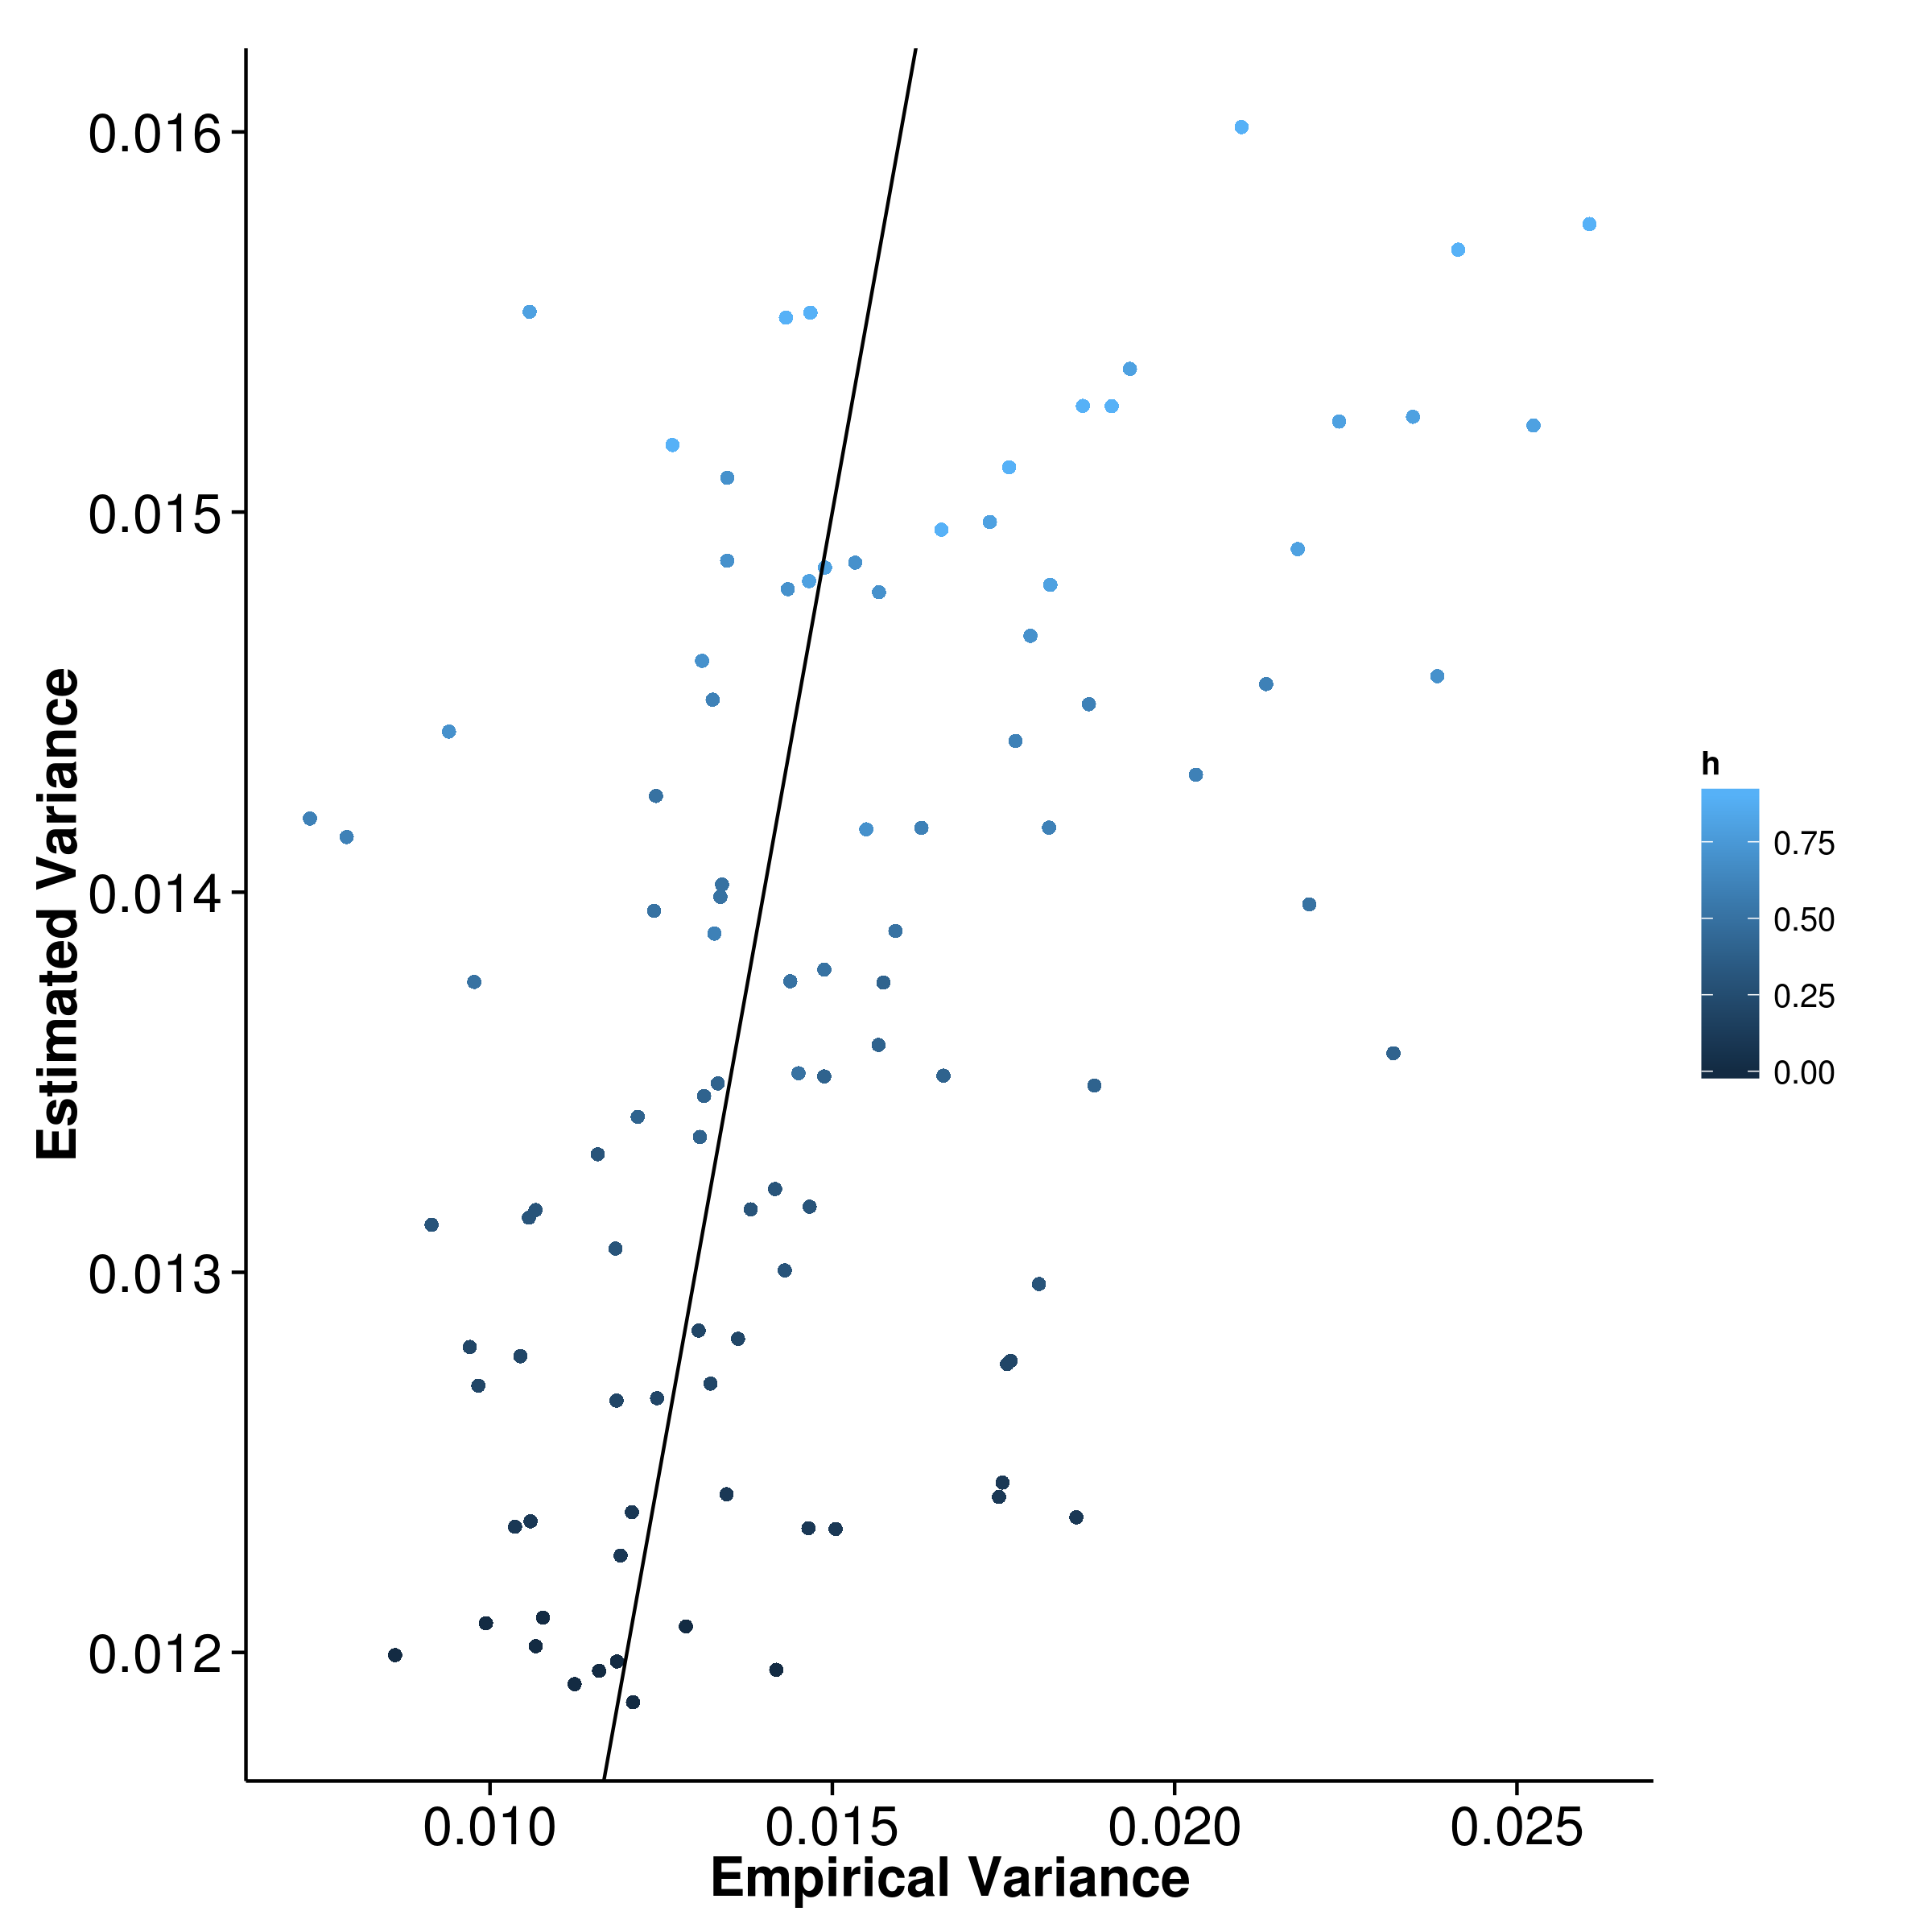
\includegraphics{figure/quantitative/same_effect/10c/shrek_50k_10c_varH.png}}
				\label{fig:50k10cQtvarS}
			}
			\subfloat[GCTA]{
				\scalebox{.4}{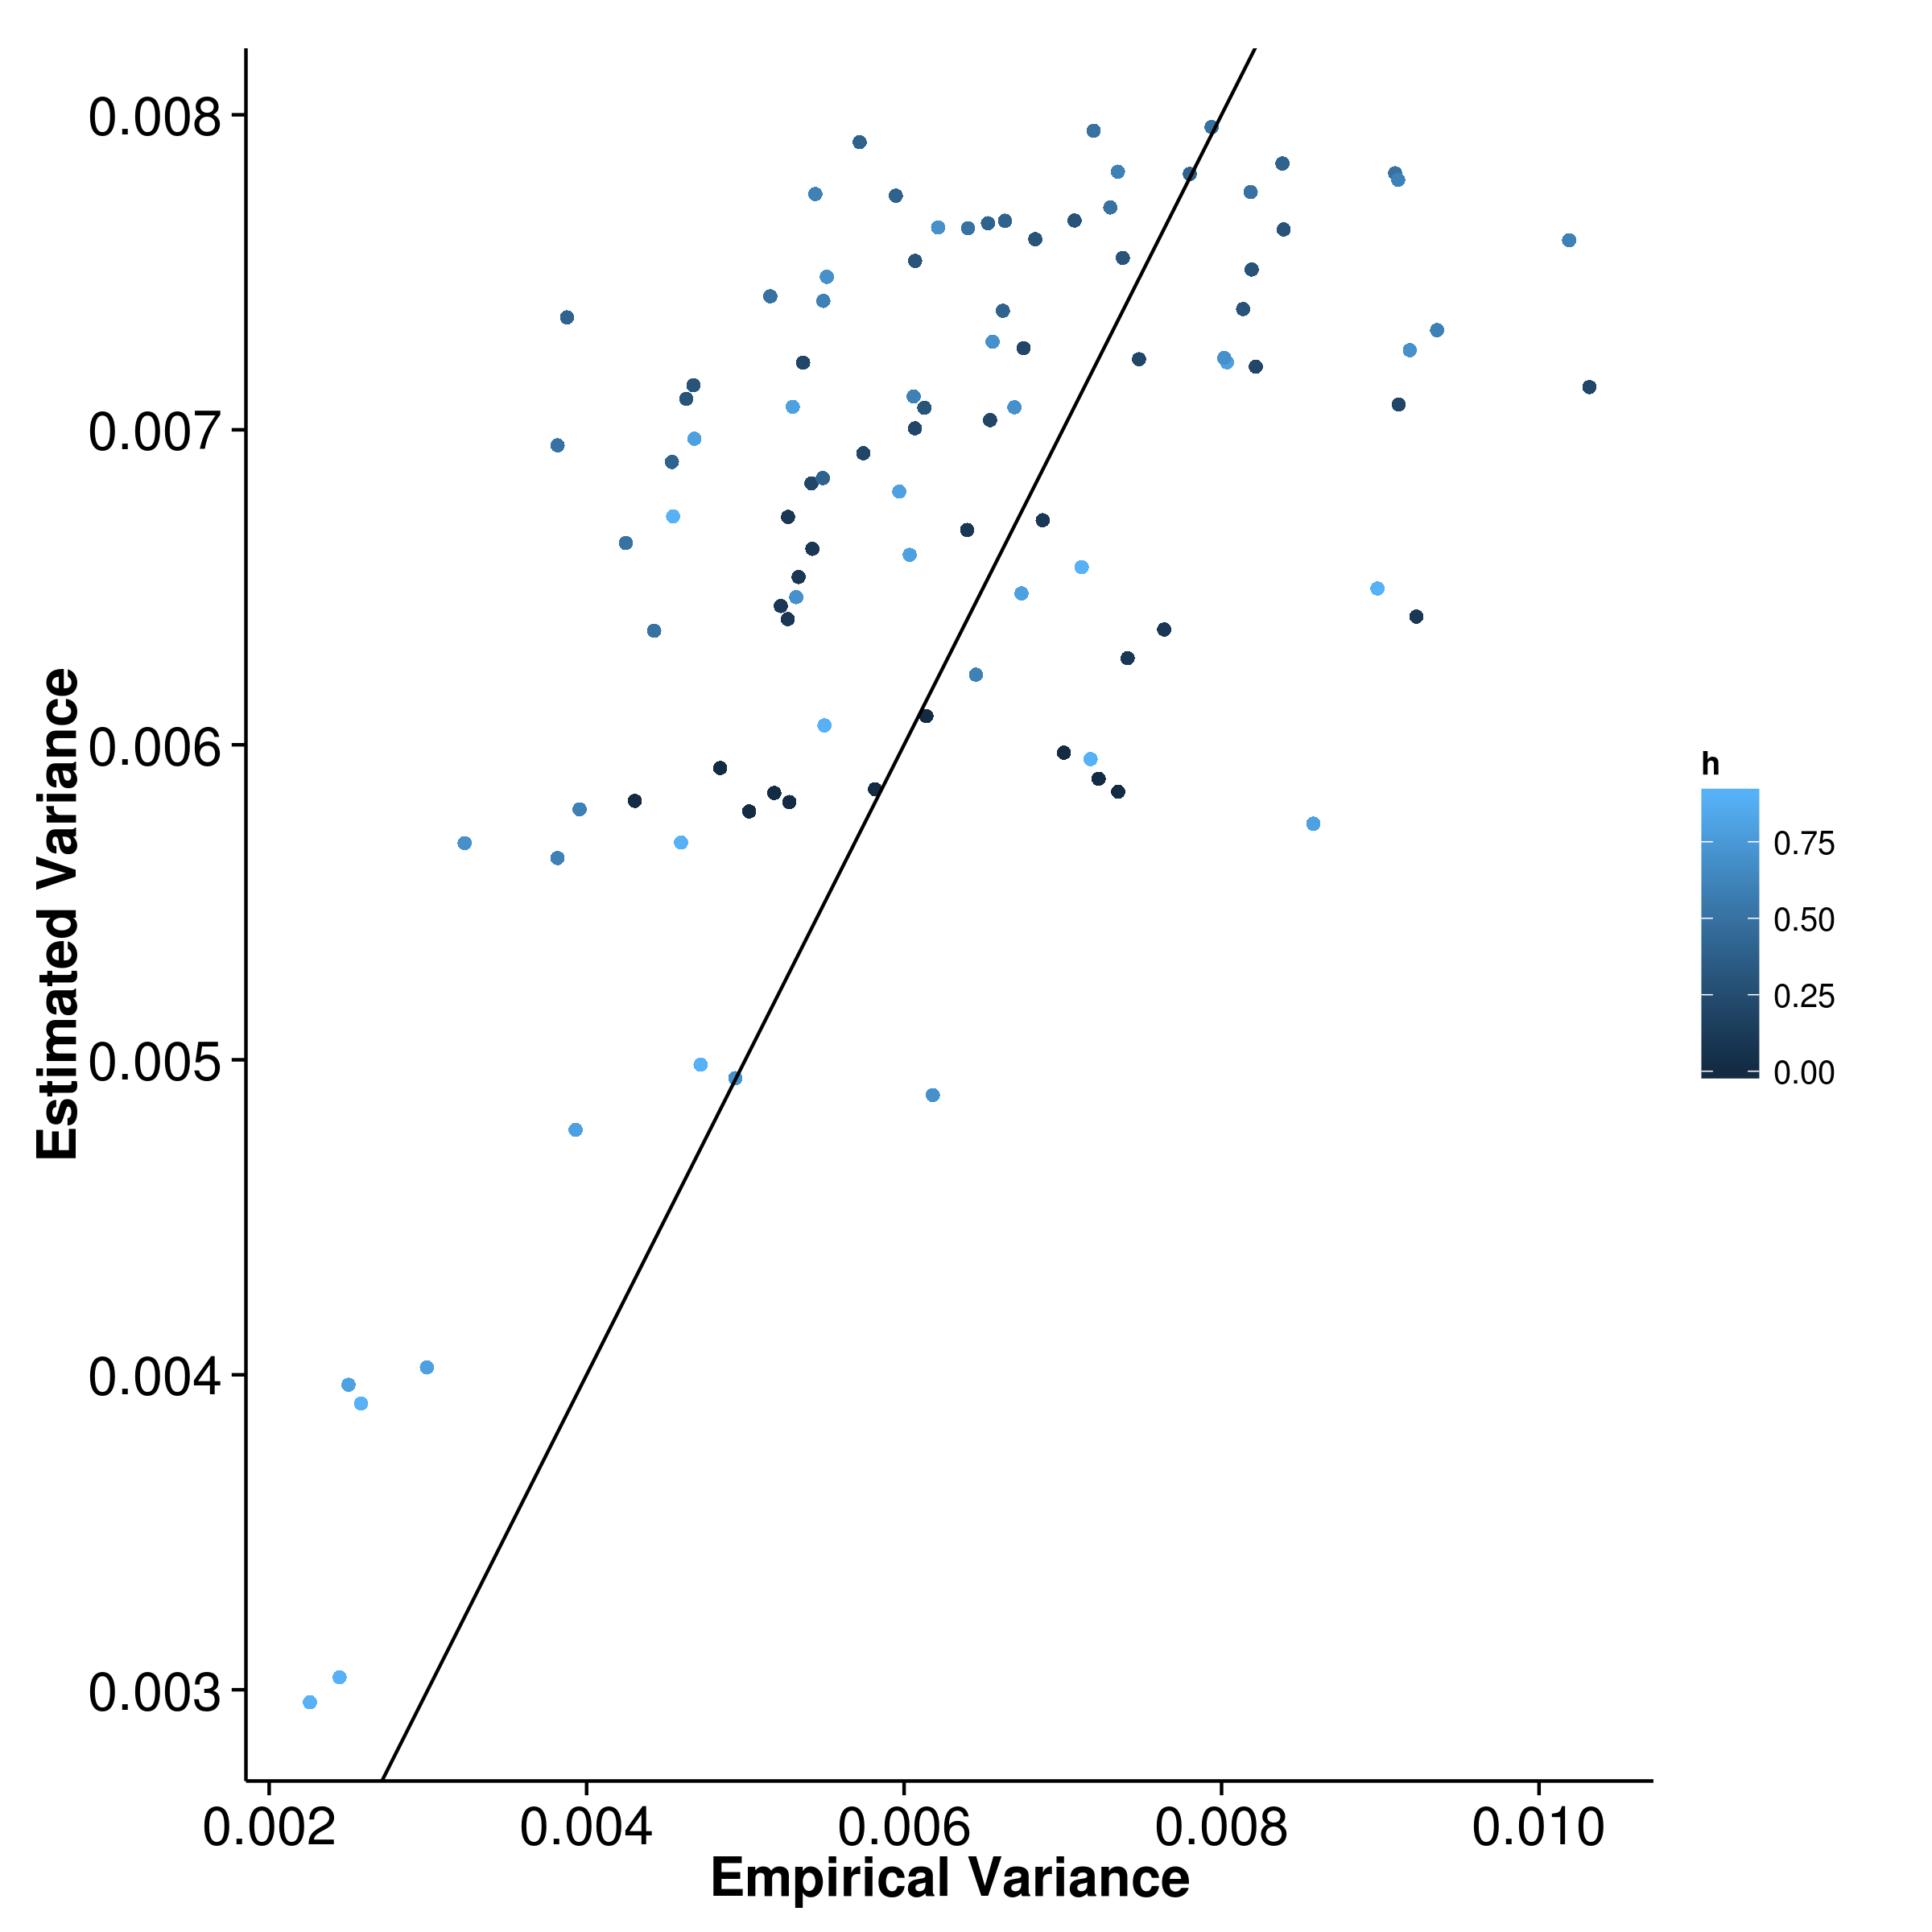
\includegraphics{figure/quantitative/same_effect/10c/gcta_50k_10c_varH.png}}
				\label{fig:50k10cQtvarG}
			}\\
			\subfloat[LDSC with fix intercept]{
				\scalebox{.4}{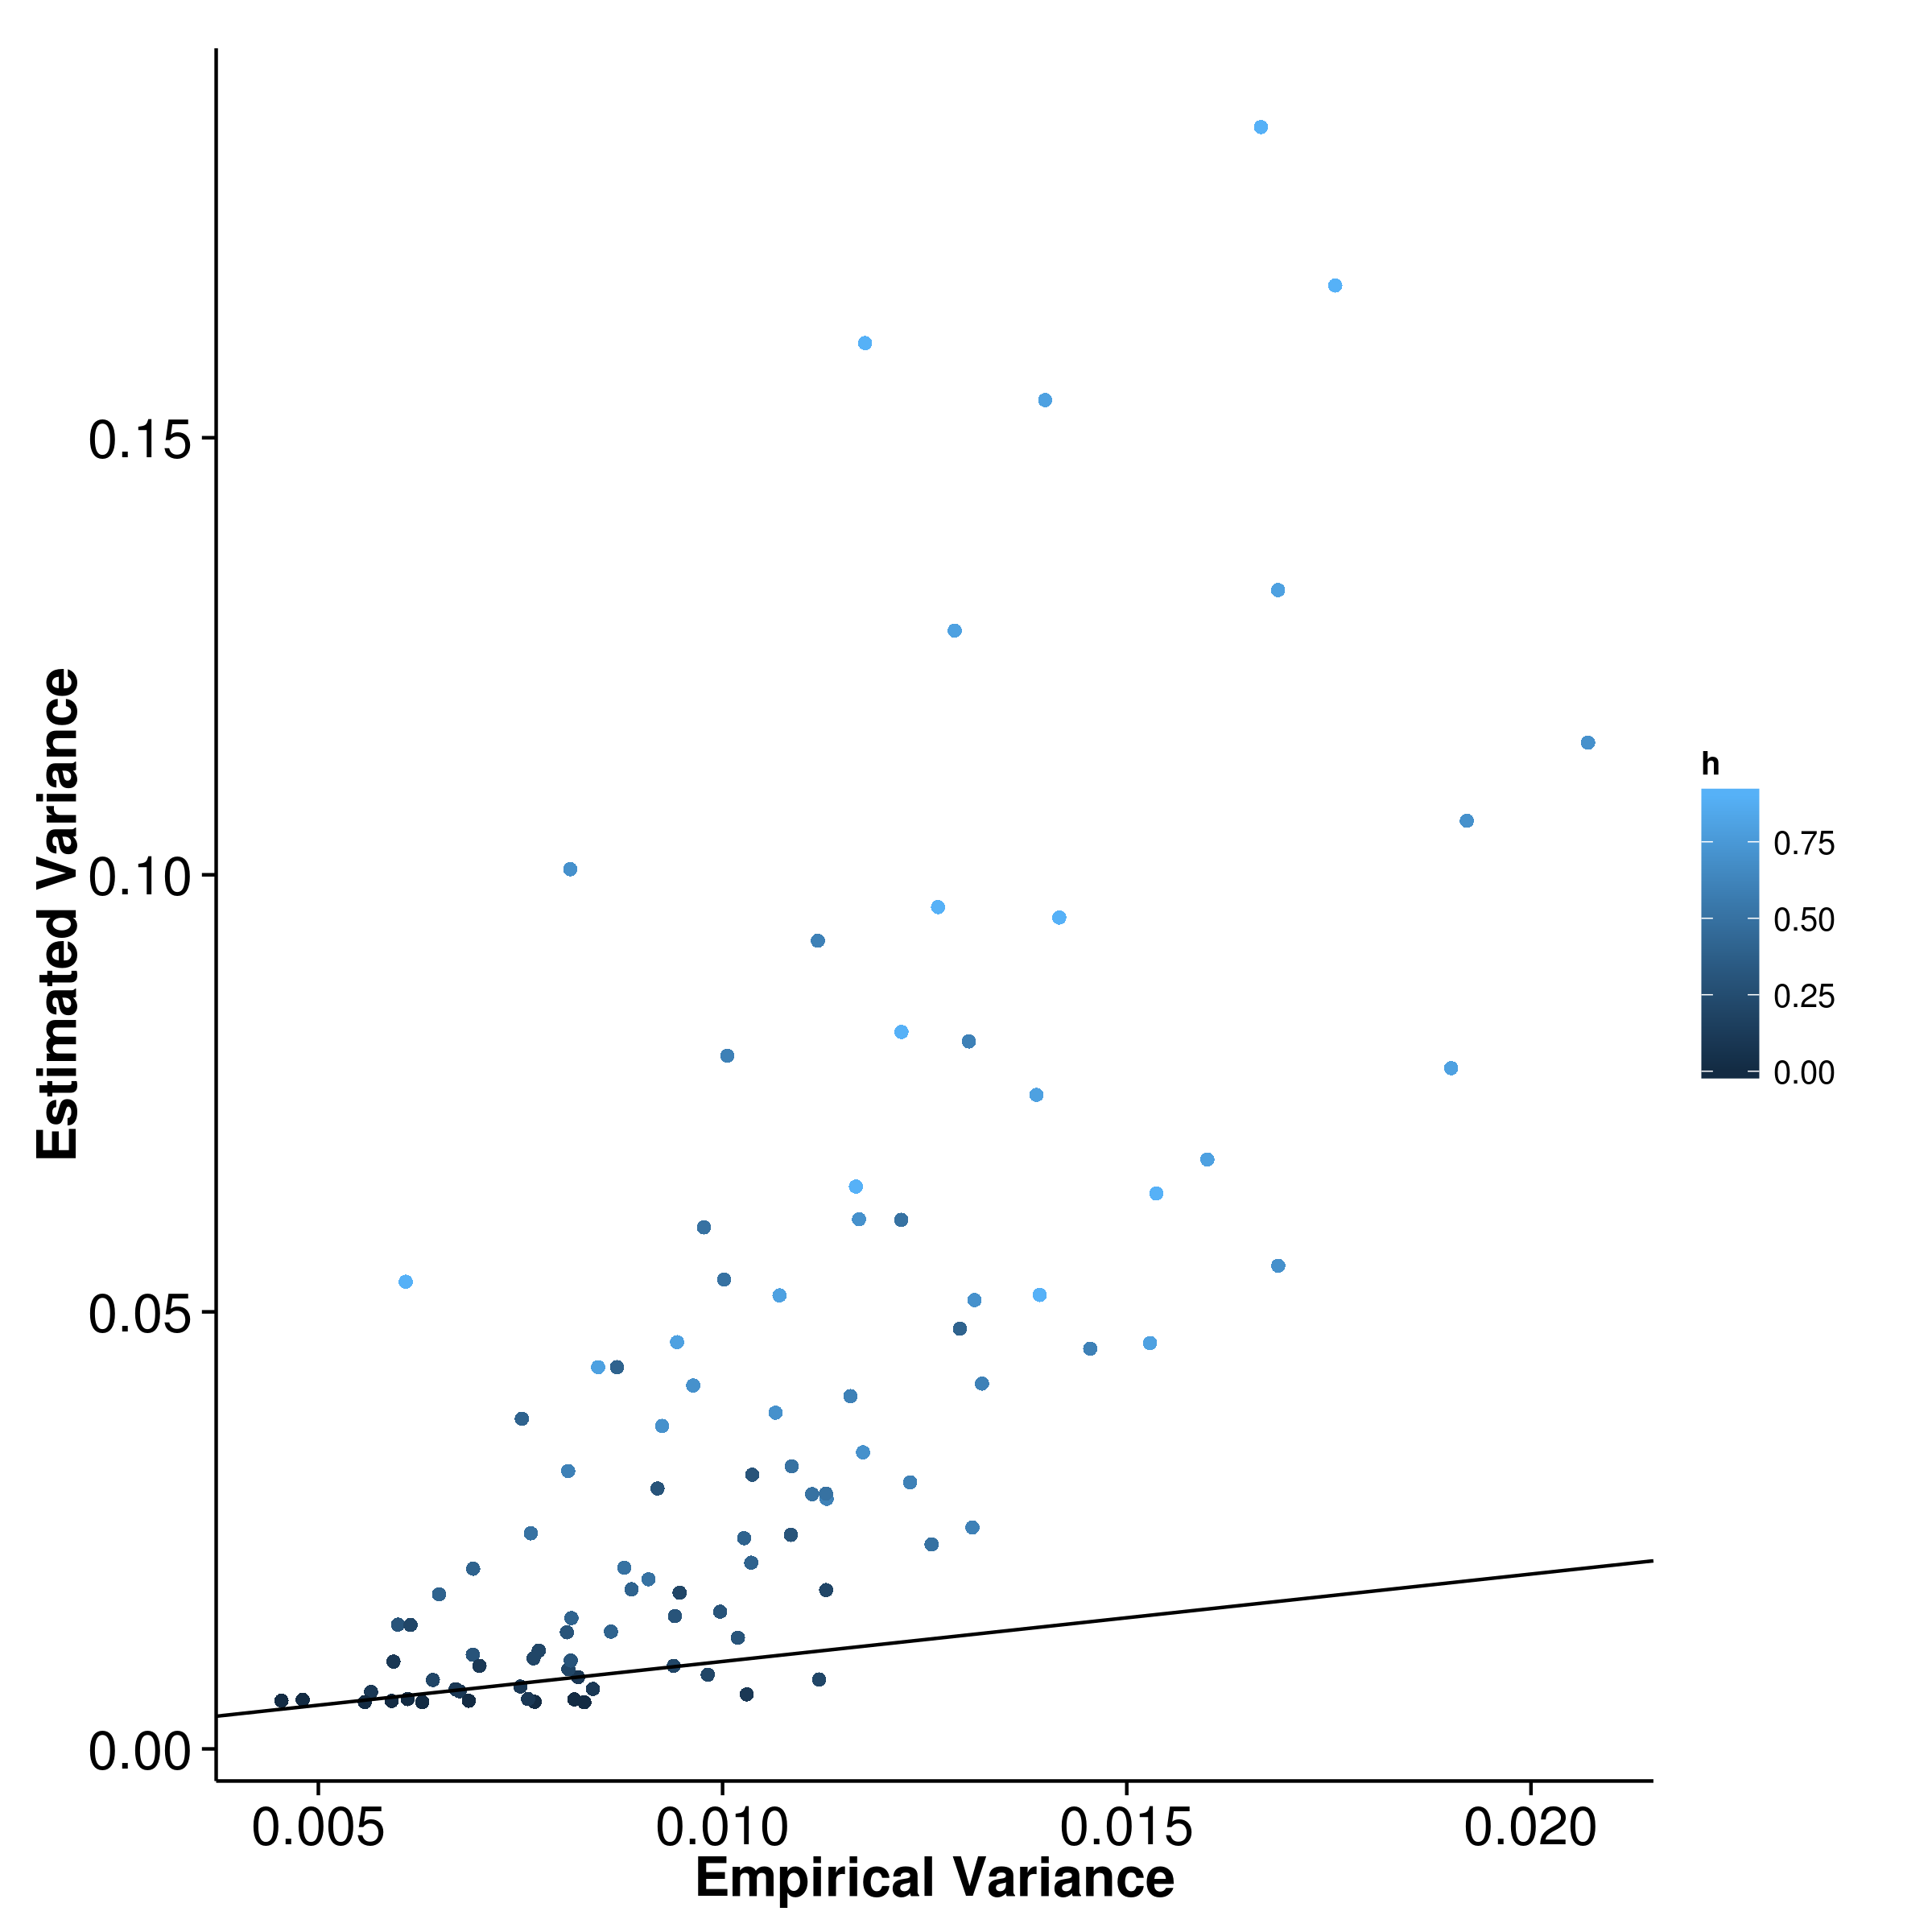
\includegraphics{figure/quantitative/same_effect/10c/ldsc_50k_10c_varH.png}}
				\label{fig:50k10cQtvarL}
			}
			\subfloat[LDSC with intercept estimation]{
				\scalebox{.4}{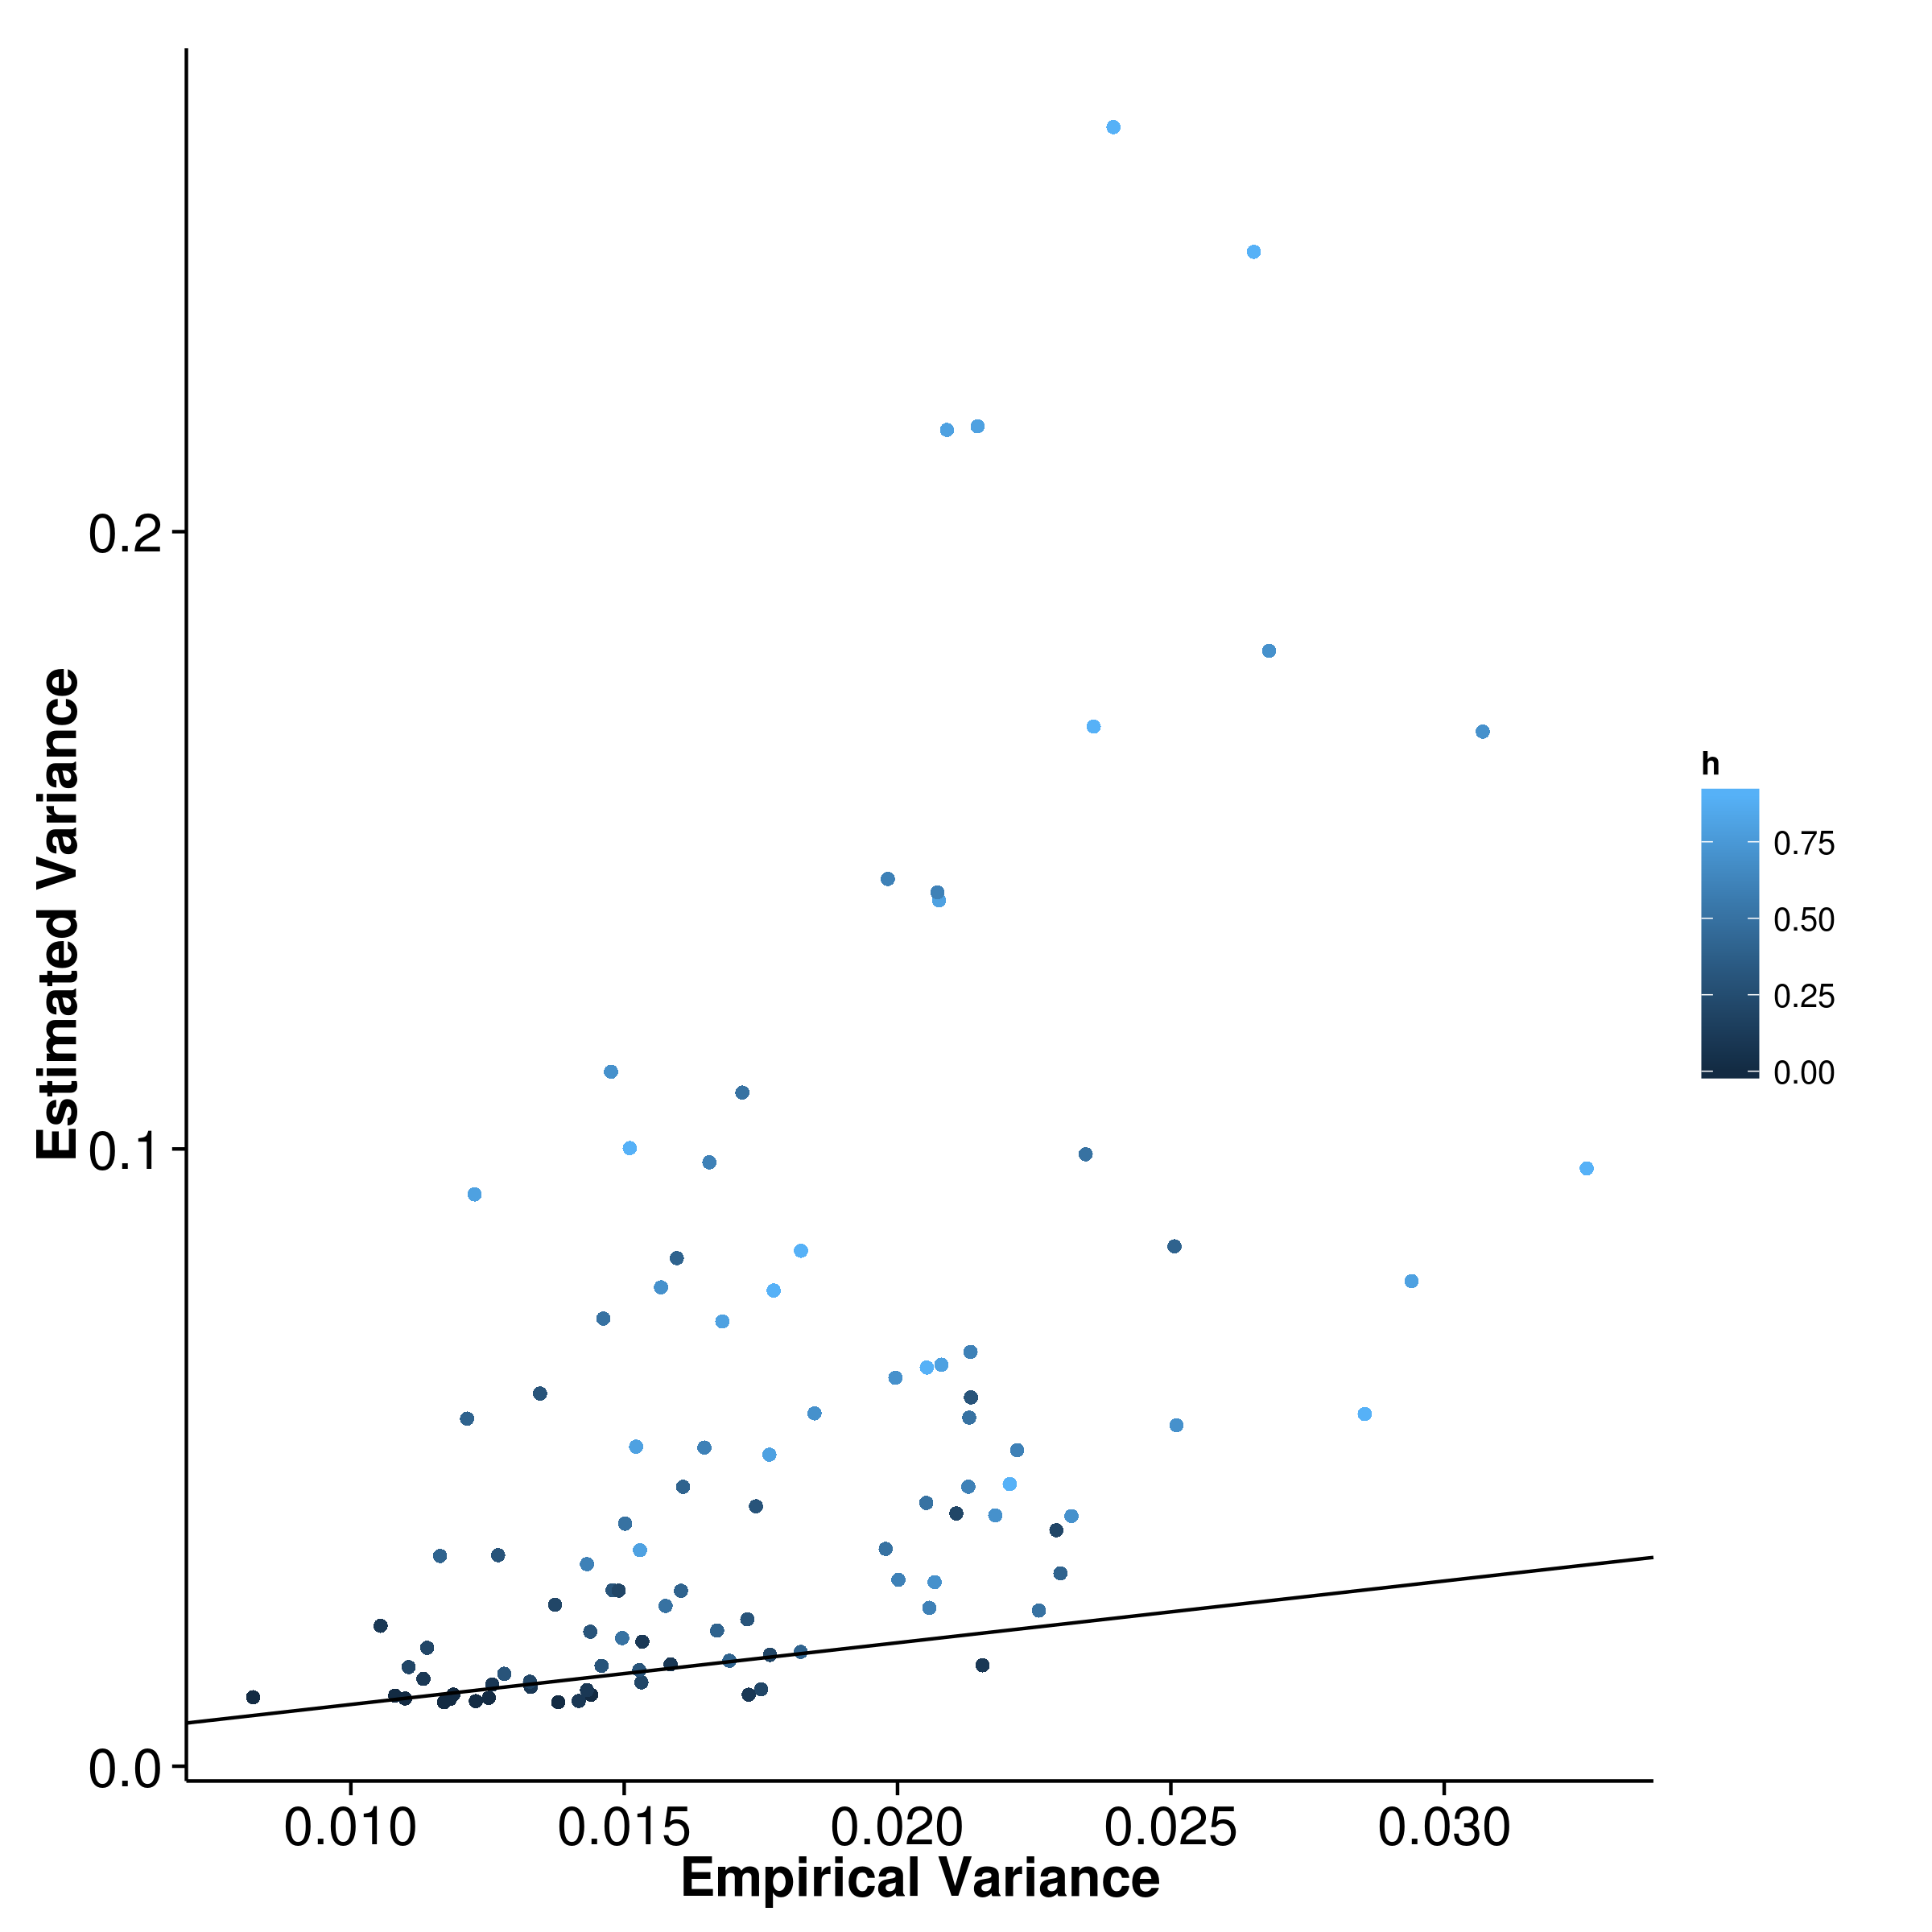
\includegraphics{figure/quantitative/same_effect/10c/ldscIn_50k_10c_varH.png}}
				\label{fig:50k10cQtvarI}
			}
			\label{fig:50k10cQtVar}
		\end{figure}
		
		
		\begin{figure}
			\centering
			\centering
			\subfloat[SHREK]{
				\scalebox{.4}{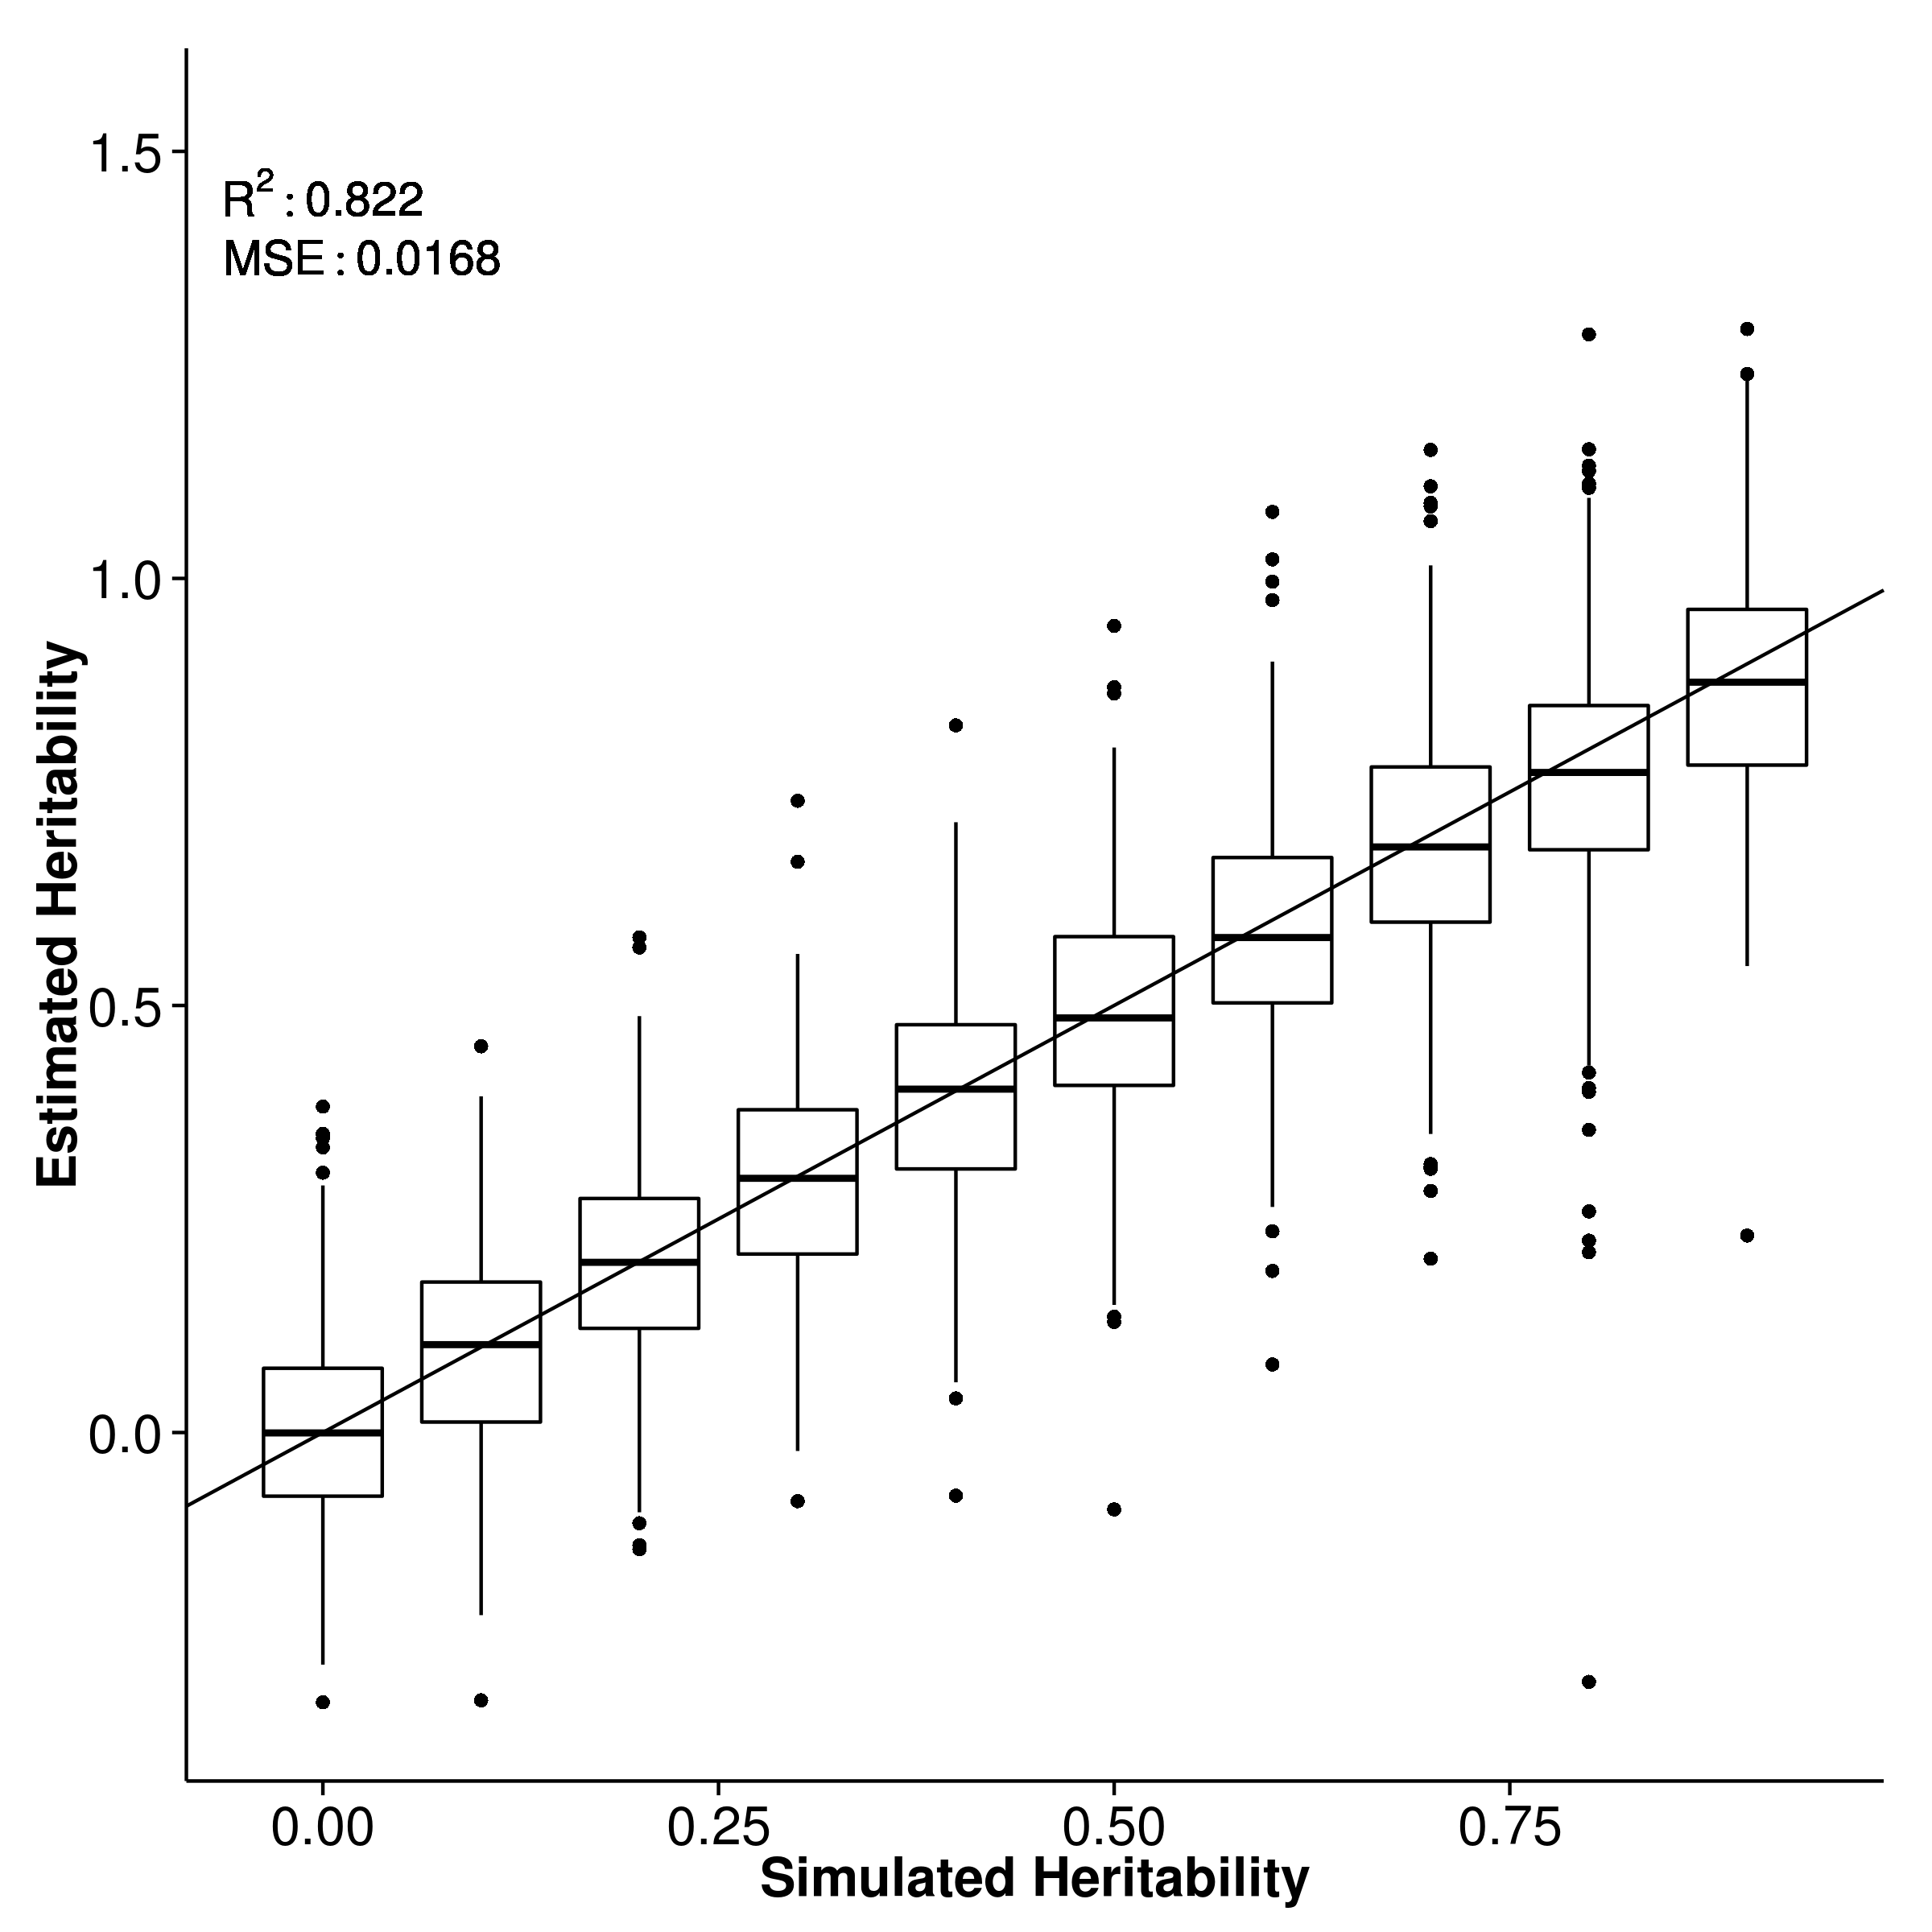
\includegraphics{figure/quantitative/same_effect/50c/shrek_50k_50c_meanH.png}}
				\label{fig:50k50cQtmeanS}
			}
			\subfloat[GCTA]{
				\scalebox{.4}{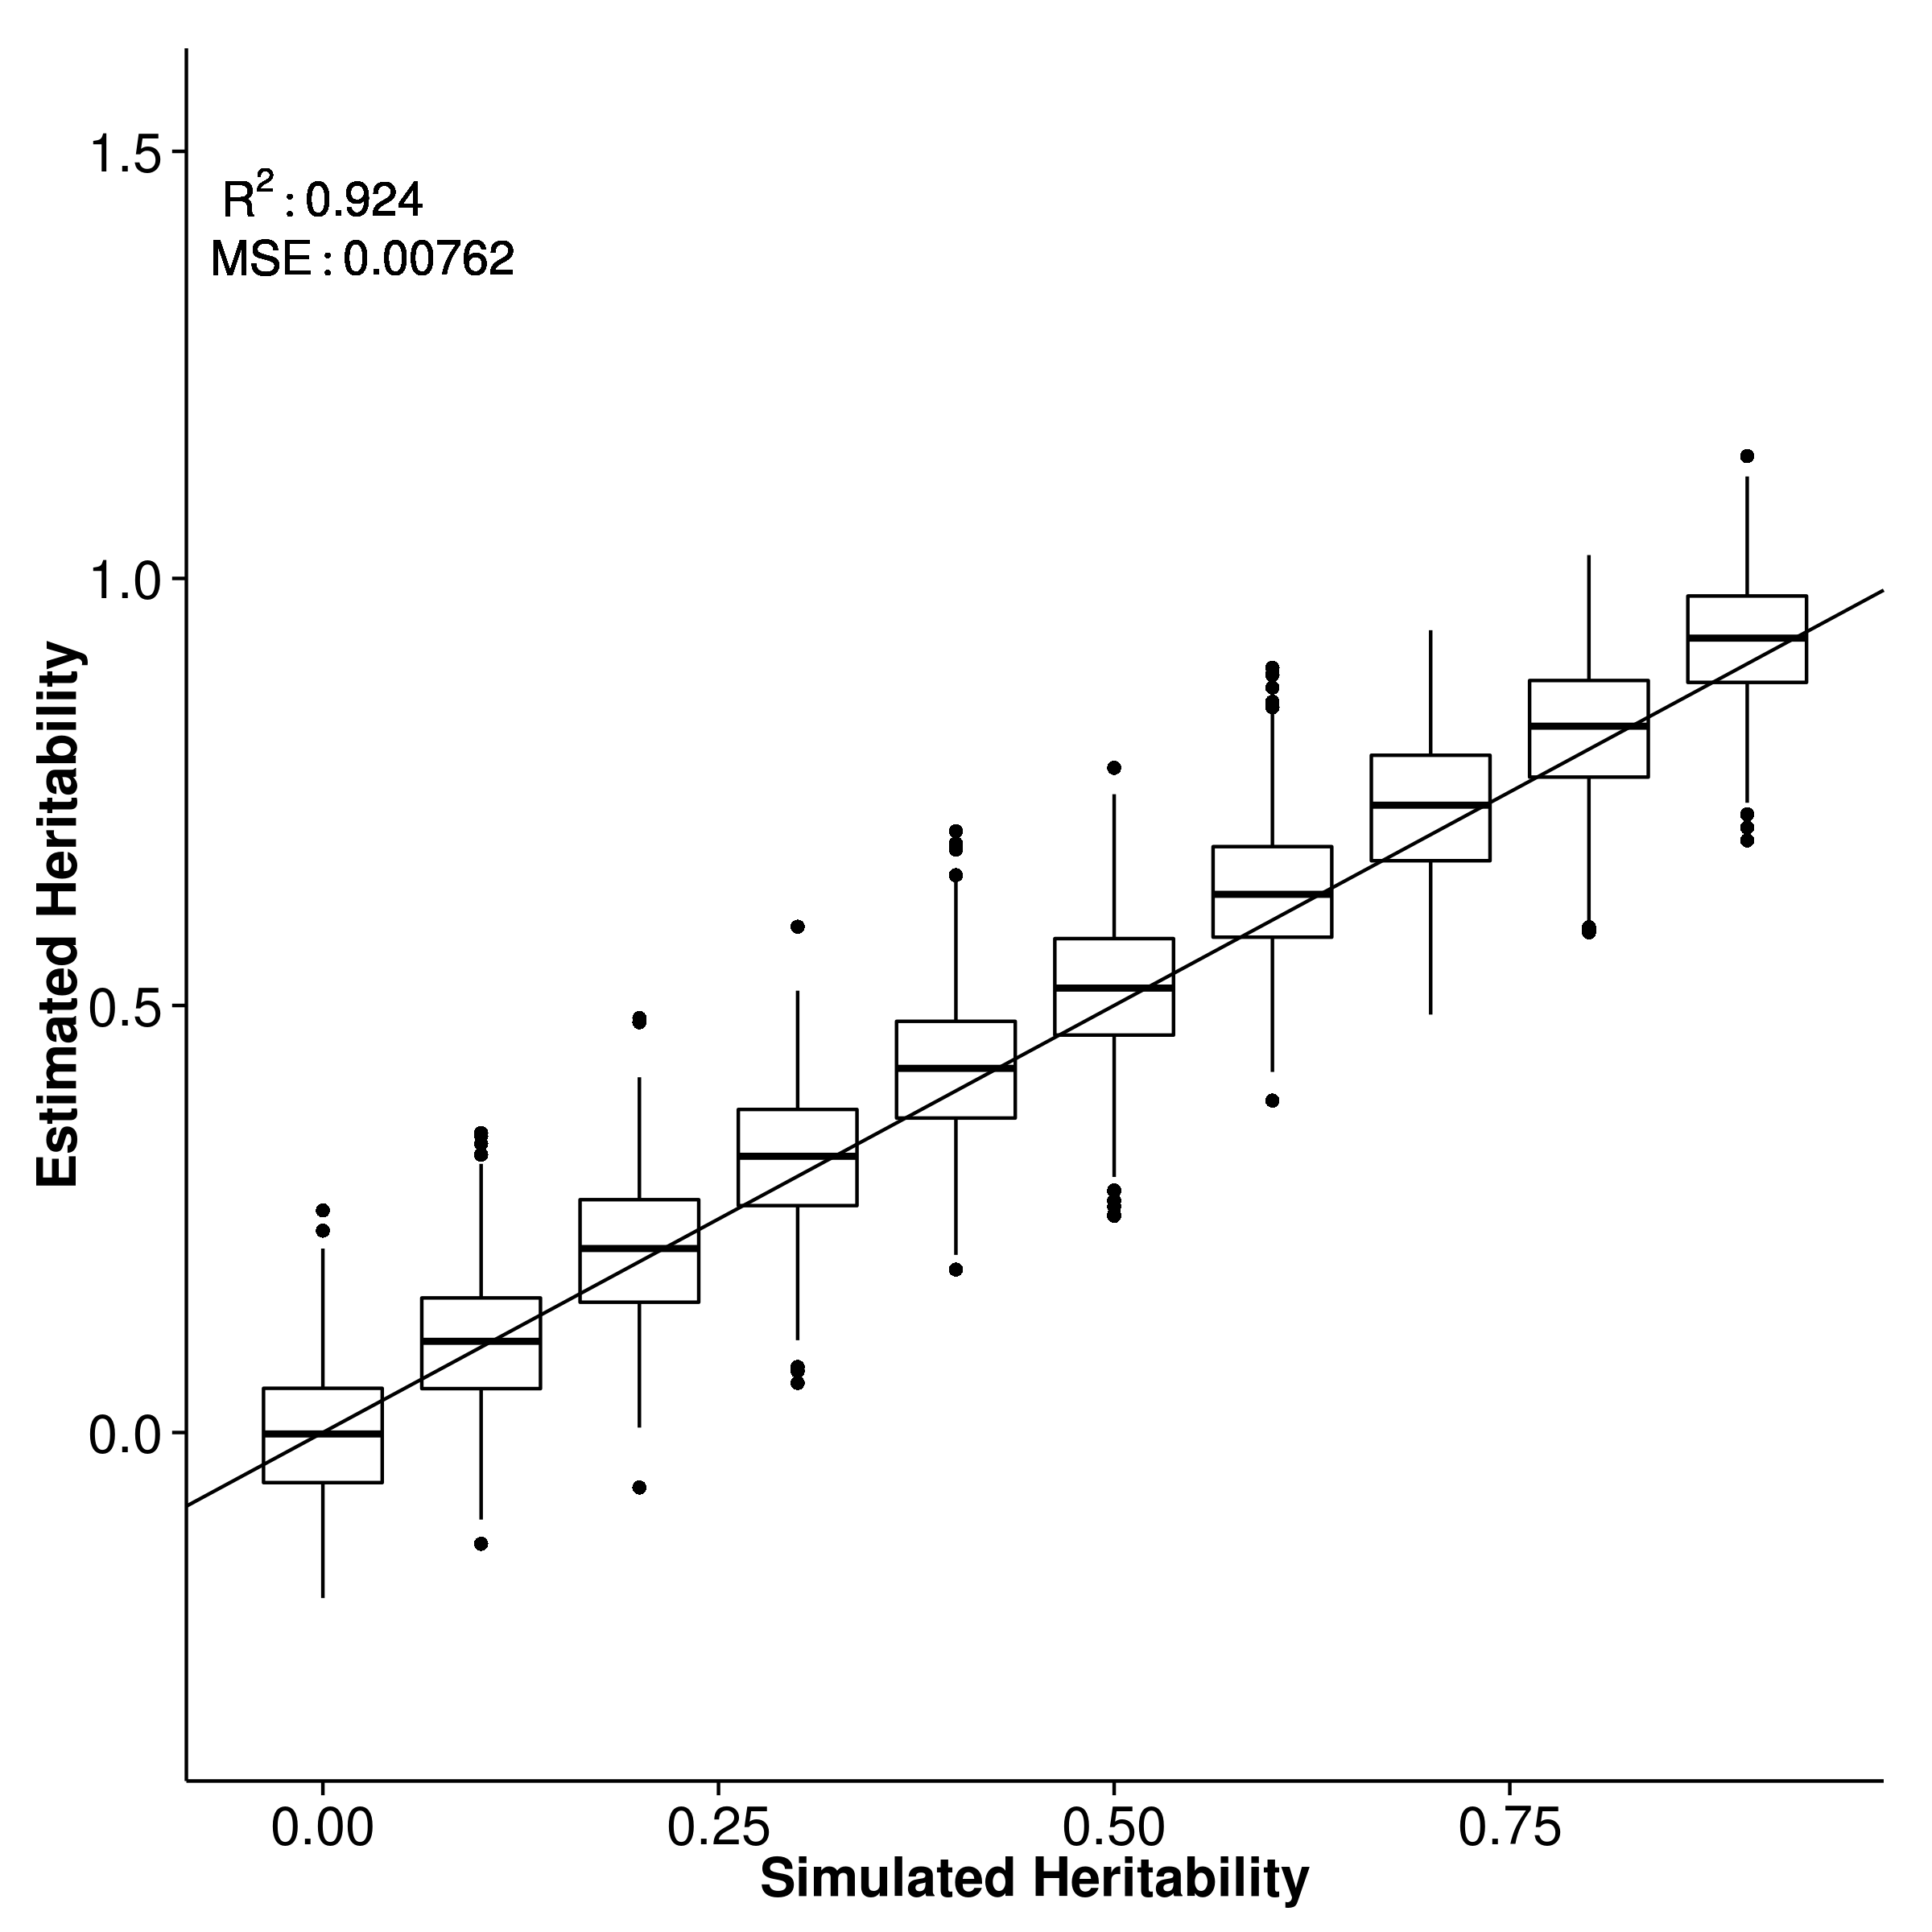
\includegraphics{figure/quantitative/same_effect/50c/gcta_50k_50c_meanH.png}}
				\label{fig:50k50cQtmeanG}
			}\\
			\subfloat[LDSC with fix intercept]{
				\scalebox{.4}{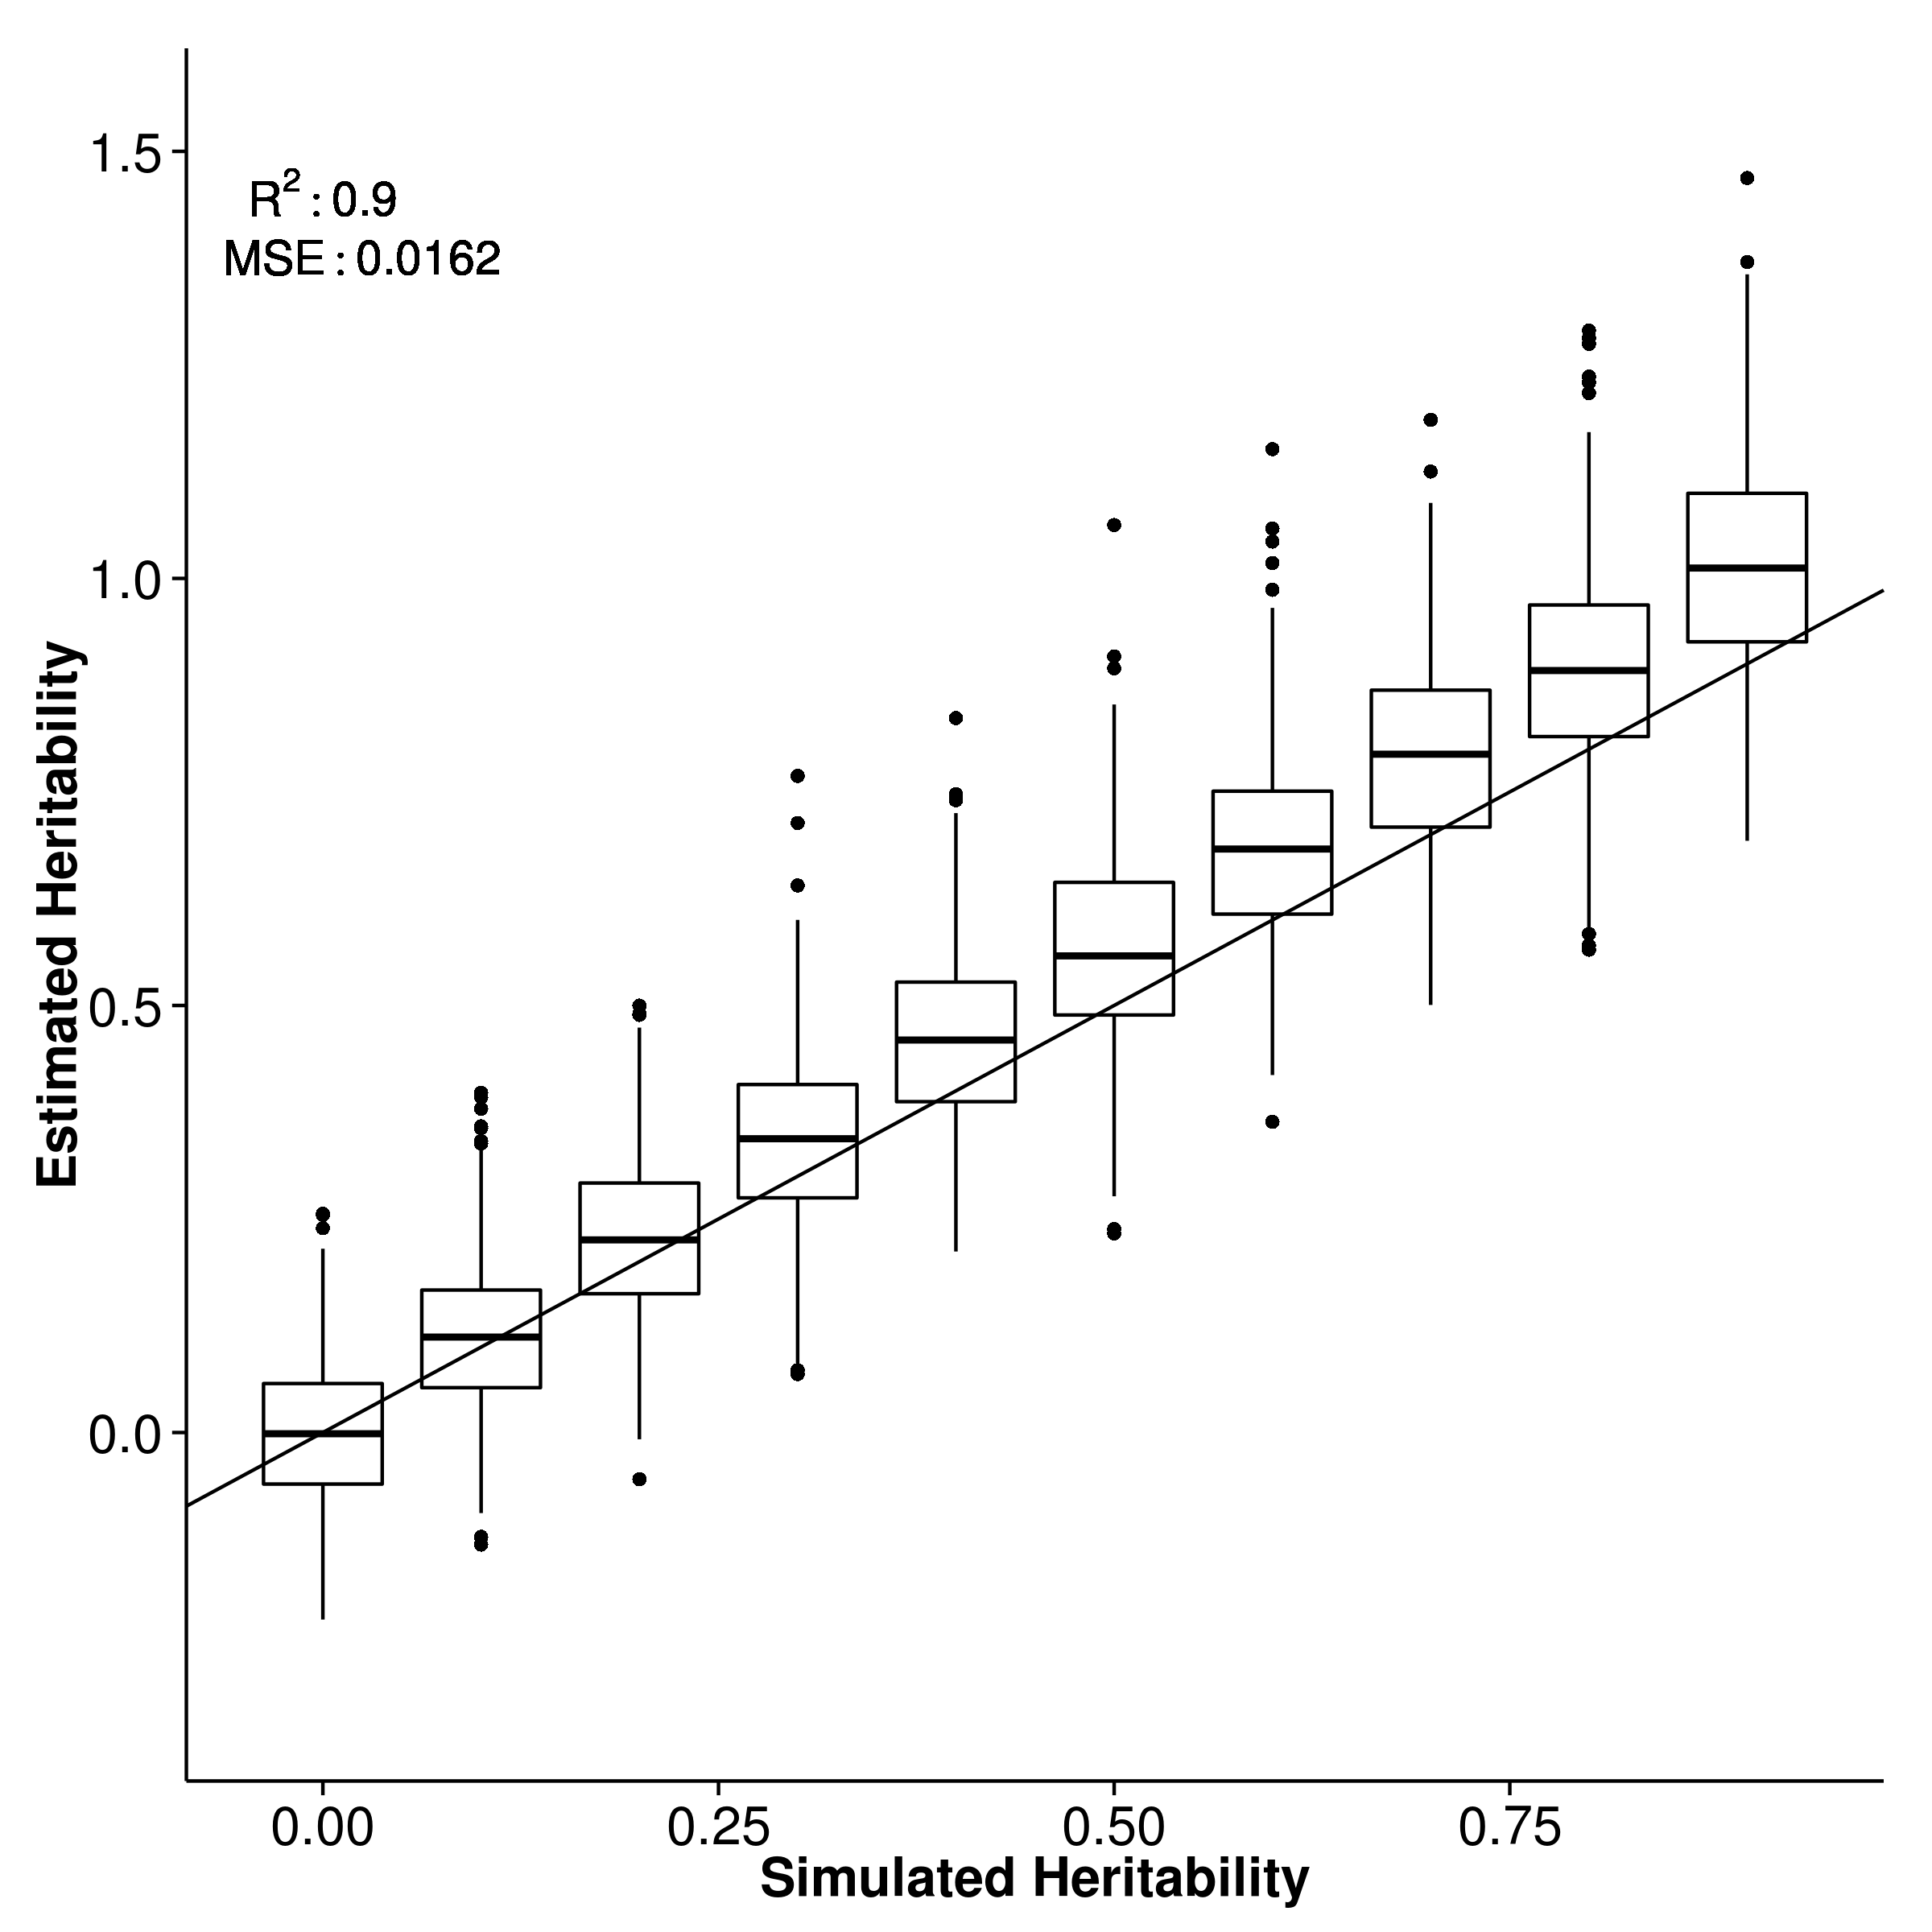
\includegraphics{figure/quantitative/same_effect/50c/ldsc_50k_50c_meanH.png}}
				\label{fig:50k50cQtmeanL}
			}
			\subfloat[LDSC with intercept estimation]{
				\scalebox{.4}{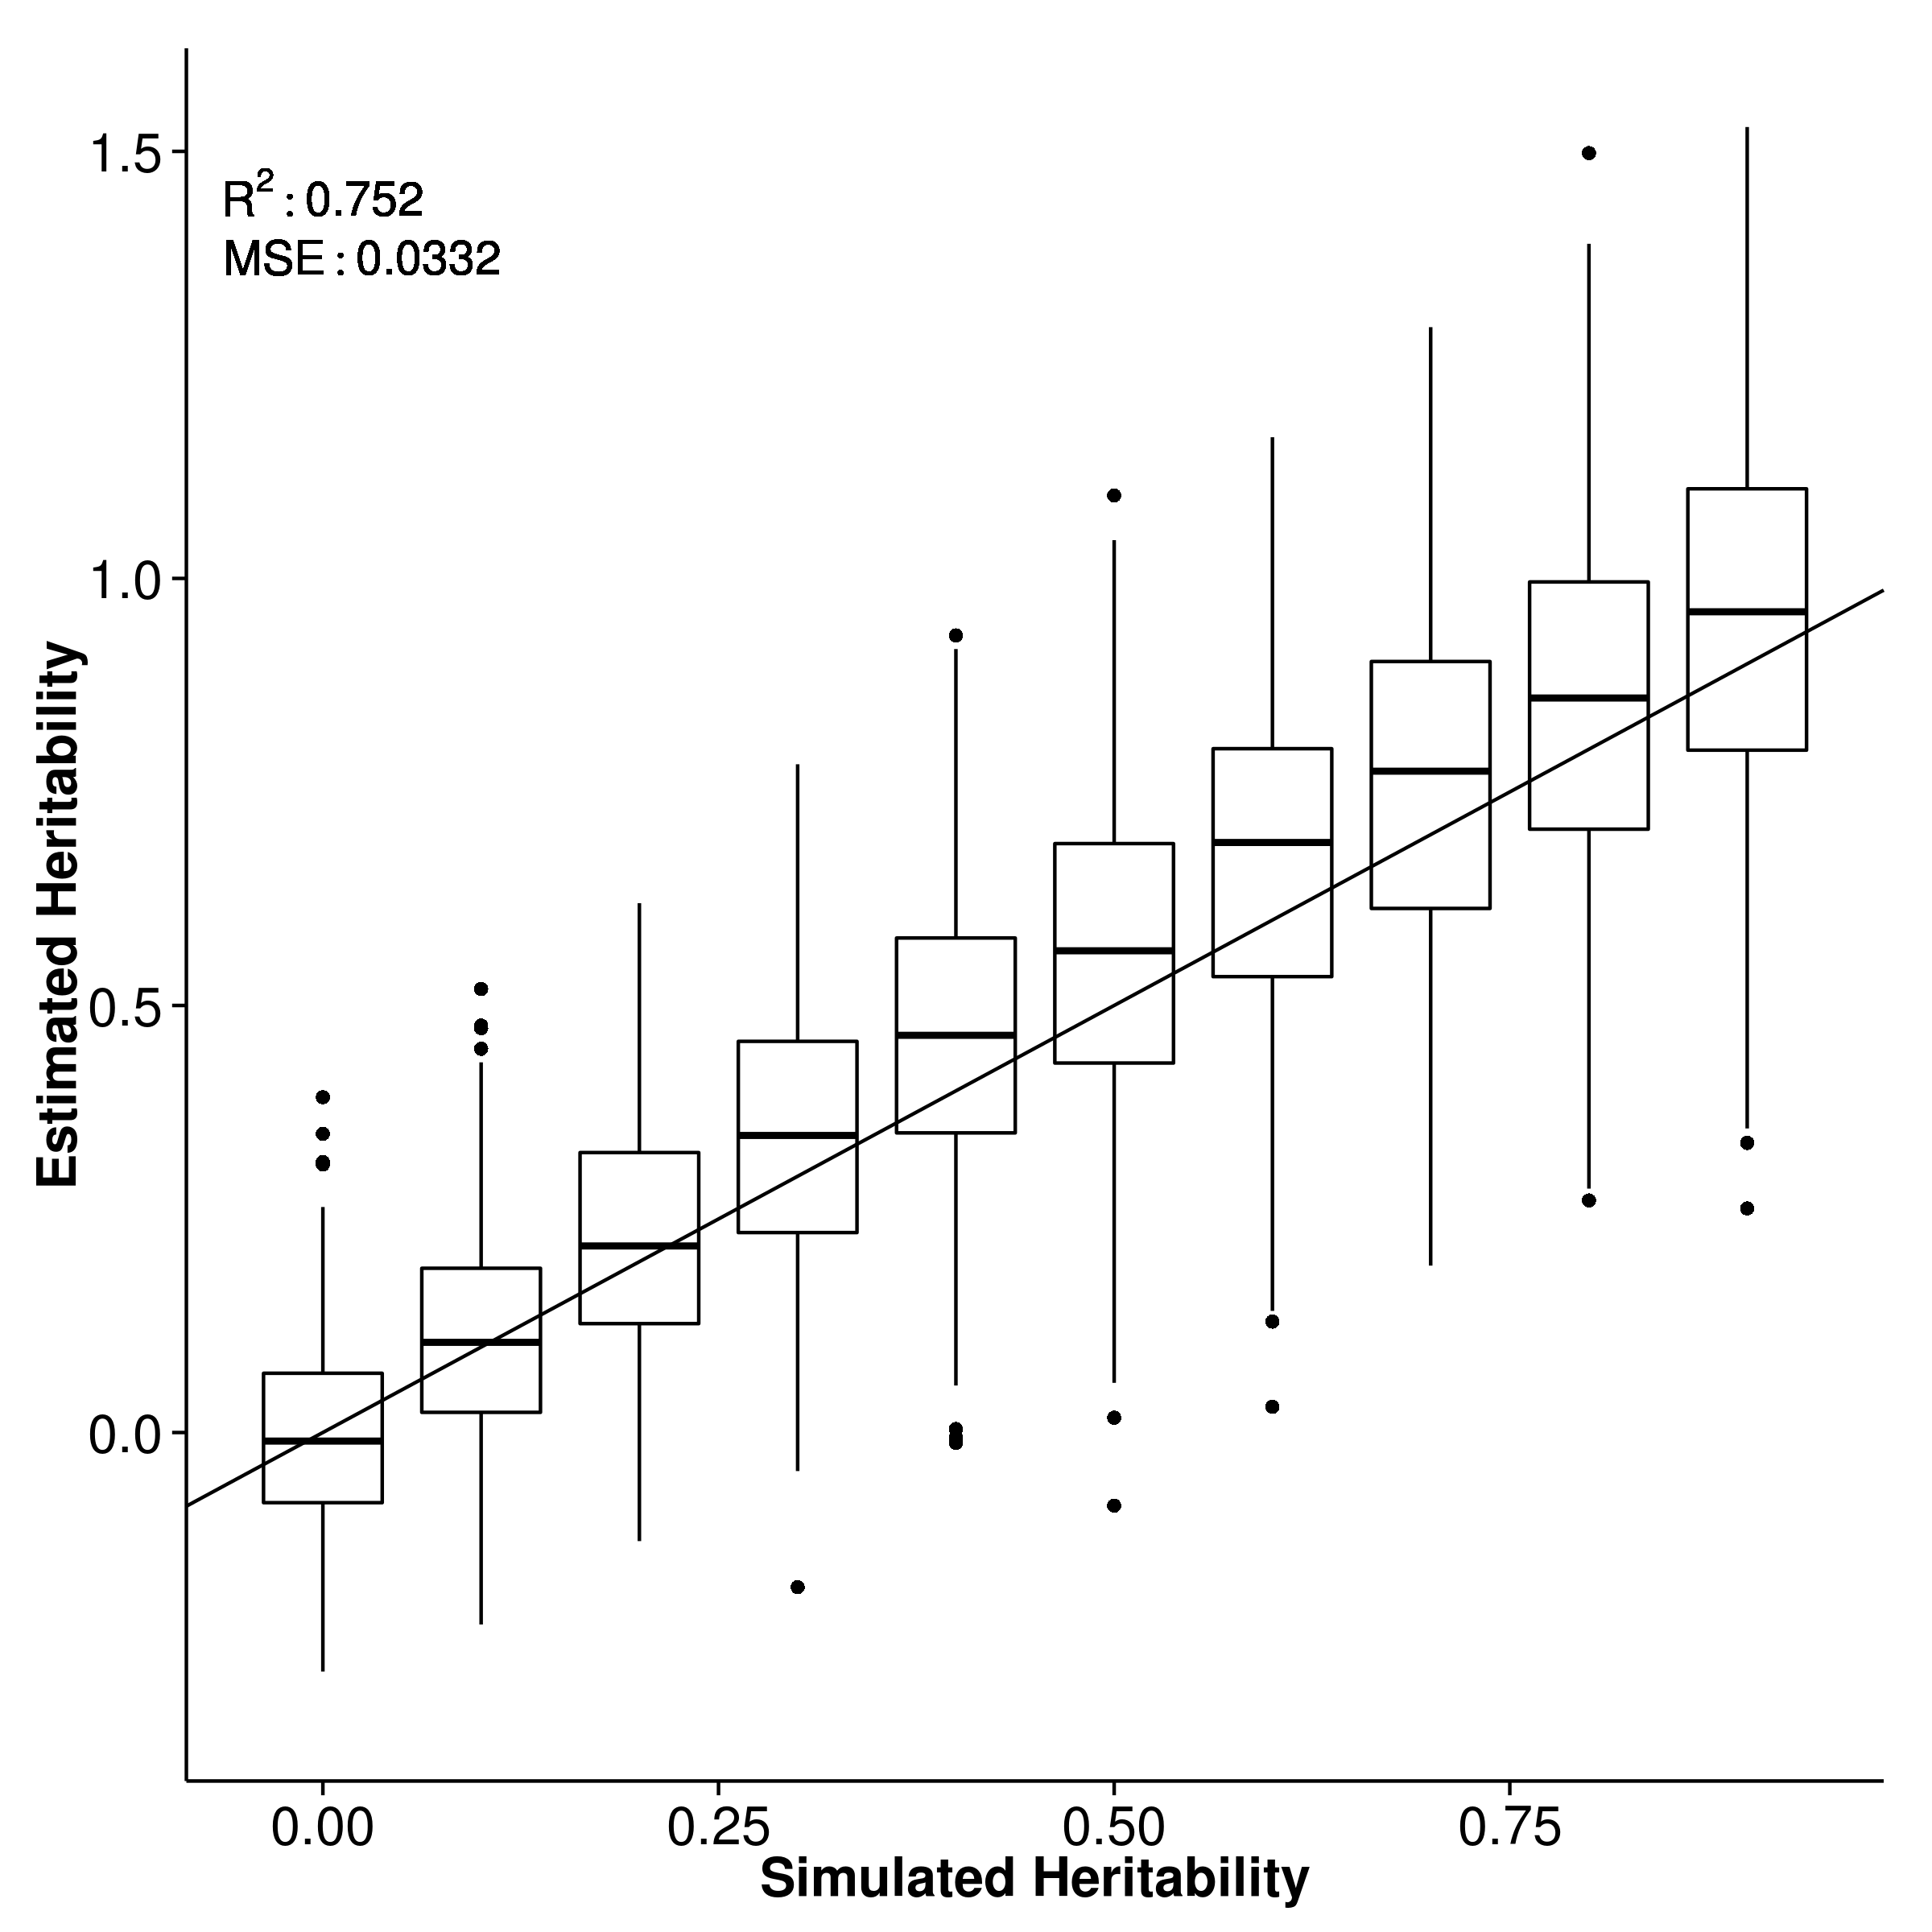
\includegraphics{figure/quantitative/same_effect/50c/ldscIn_50k_50c_meanH.png}}
				\label{fig:50k50cQtmeanI}
			}
			\caption[Simulation of Quantitative Traits with 50k \glsentryshortpl{SNP} and 50 causal variants of same effect size]
			{Simulation of Quantitative Traits with 50k \glsentryshortpl{SNP} and 50 causal variants with same effect size.} 
			\label{fig:50k50cQtMean}
		\end{figure}
		\begin{figure}
			\centering
			\centering
			\subfloat[SHREK]{
				\scalebox{.4}{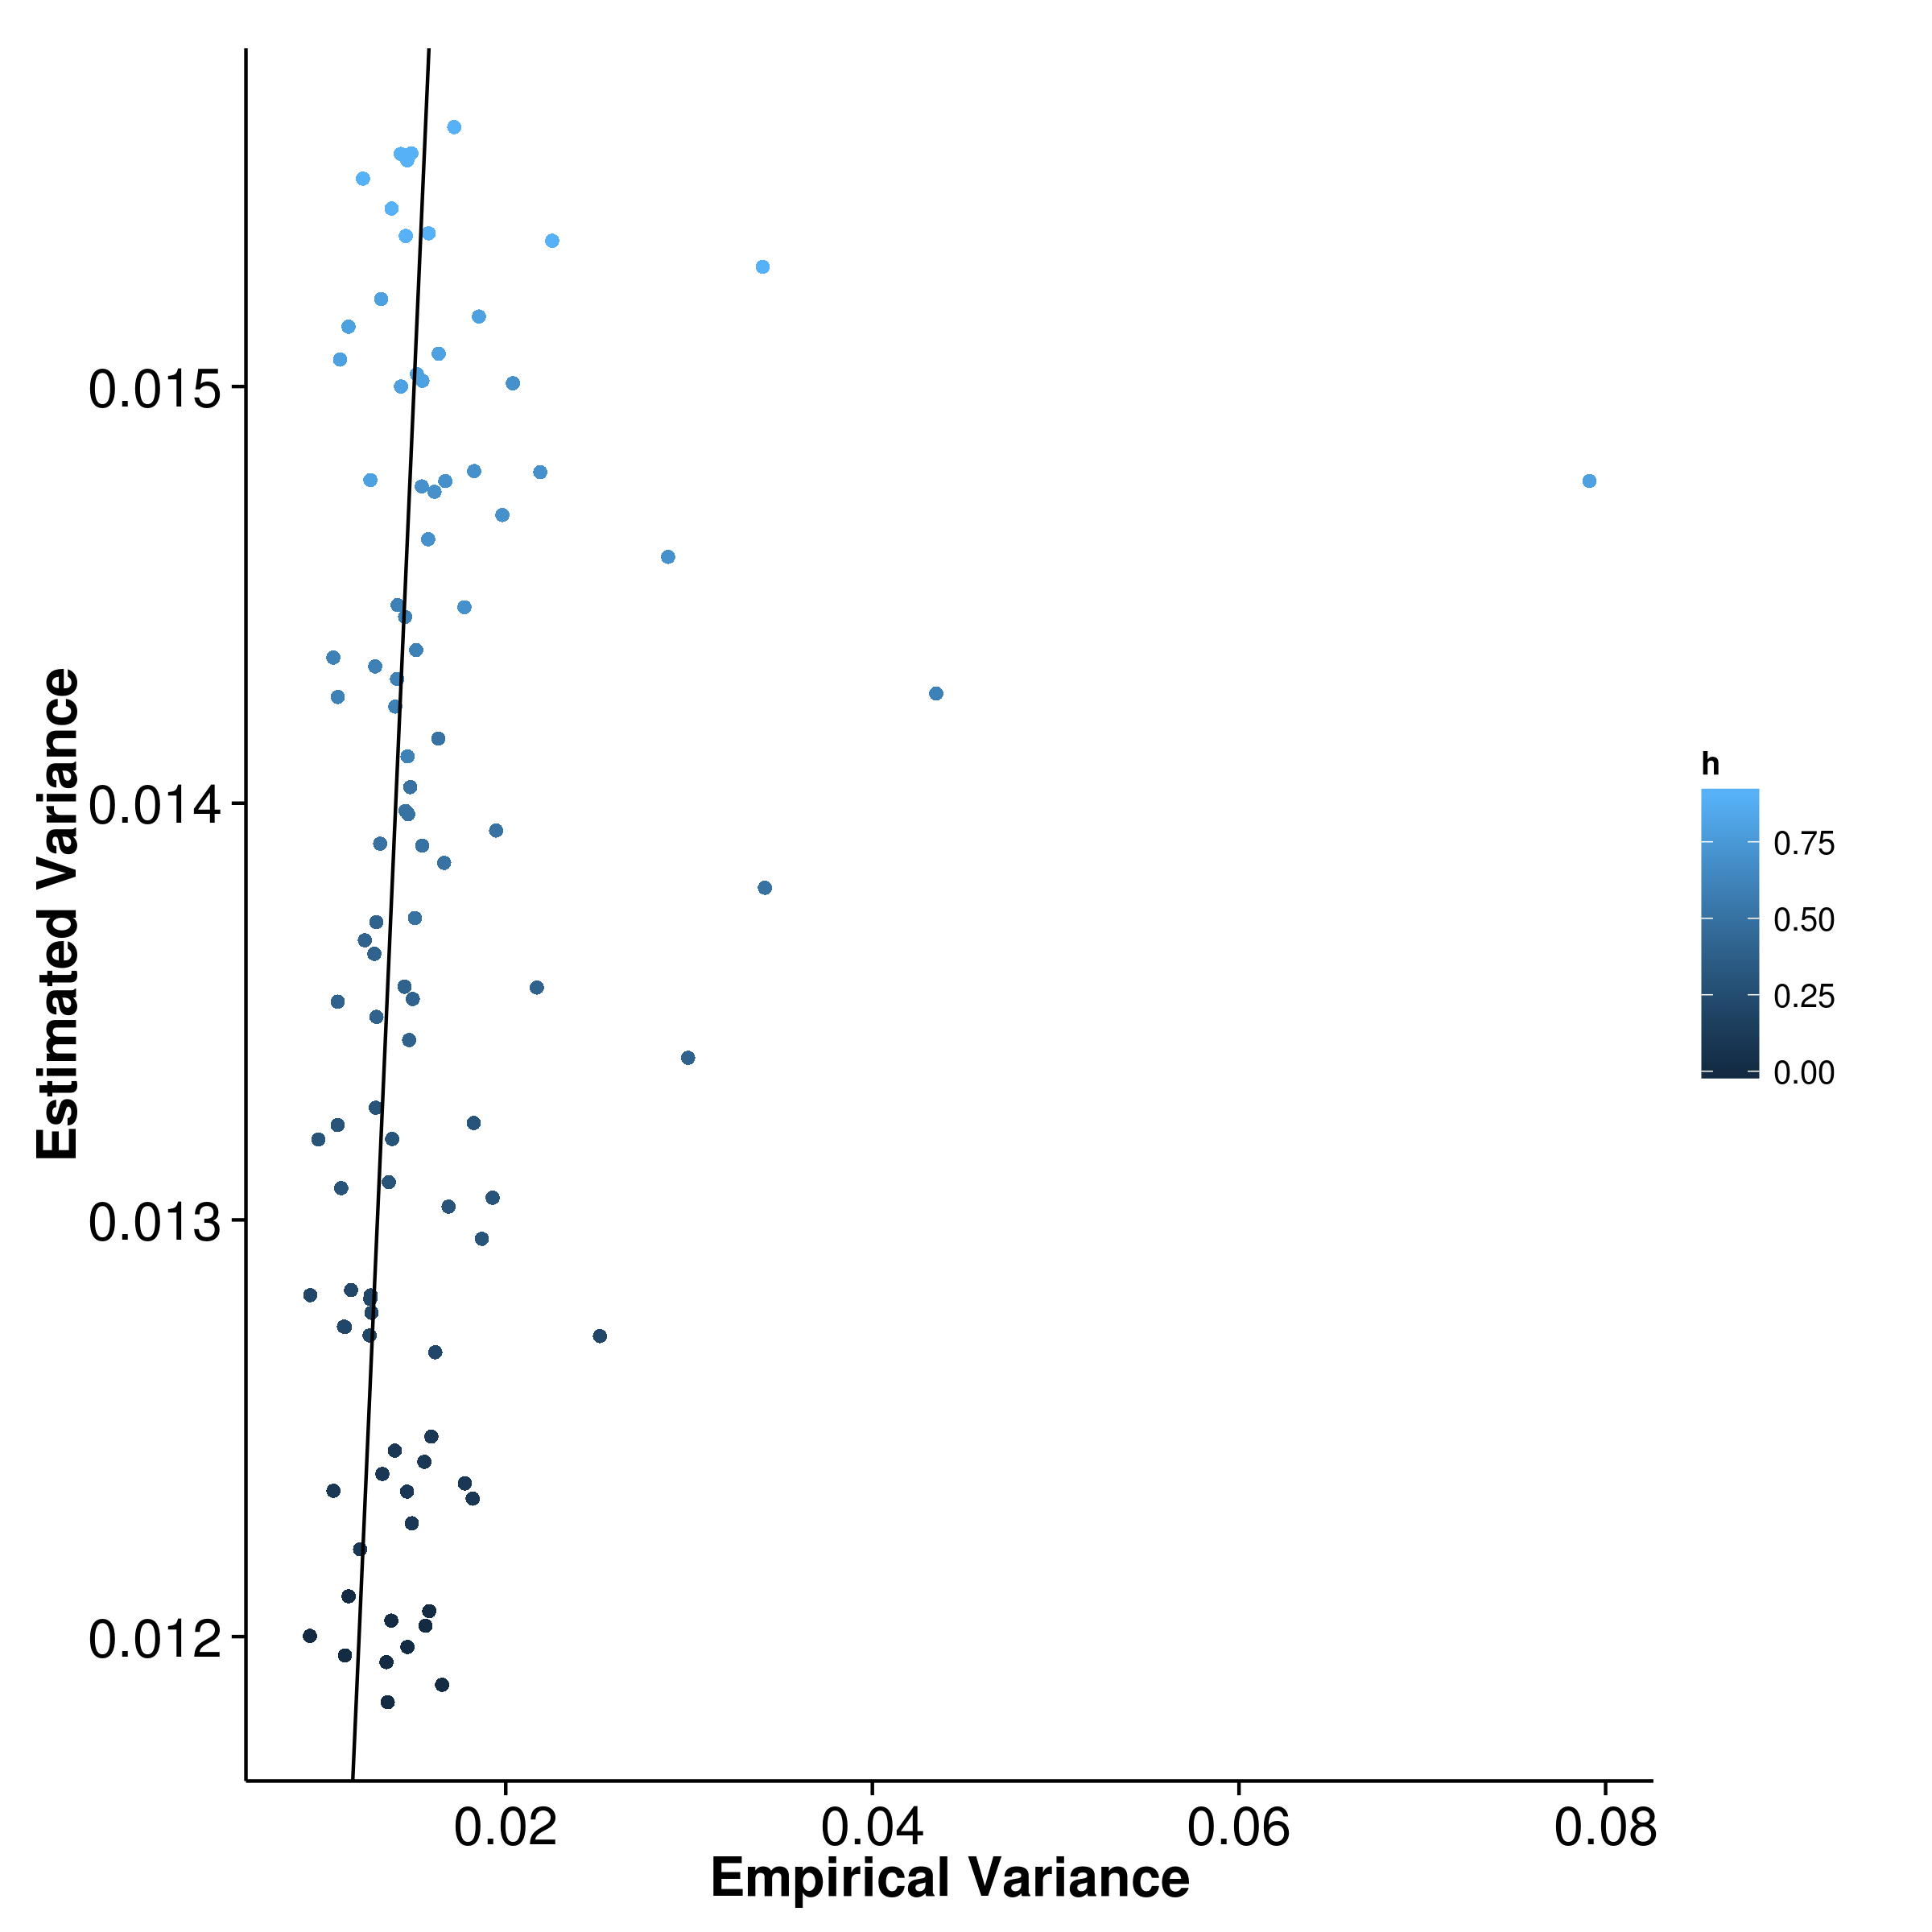
\includegraphics{figure/quantitative/same_effect/50c/shrek_50k_50c_varH.png}}
				\label{fig:50k50cQtvarS}
			}
			\subfloat[GCTA]{
				\scalebox{.4}{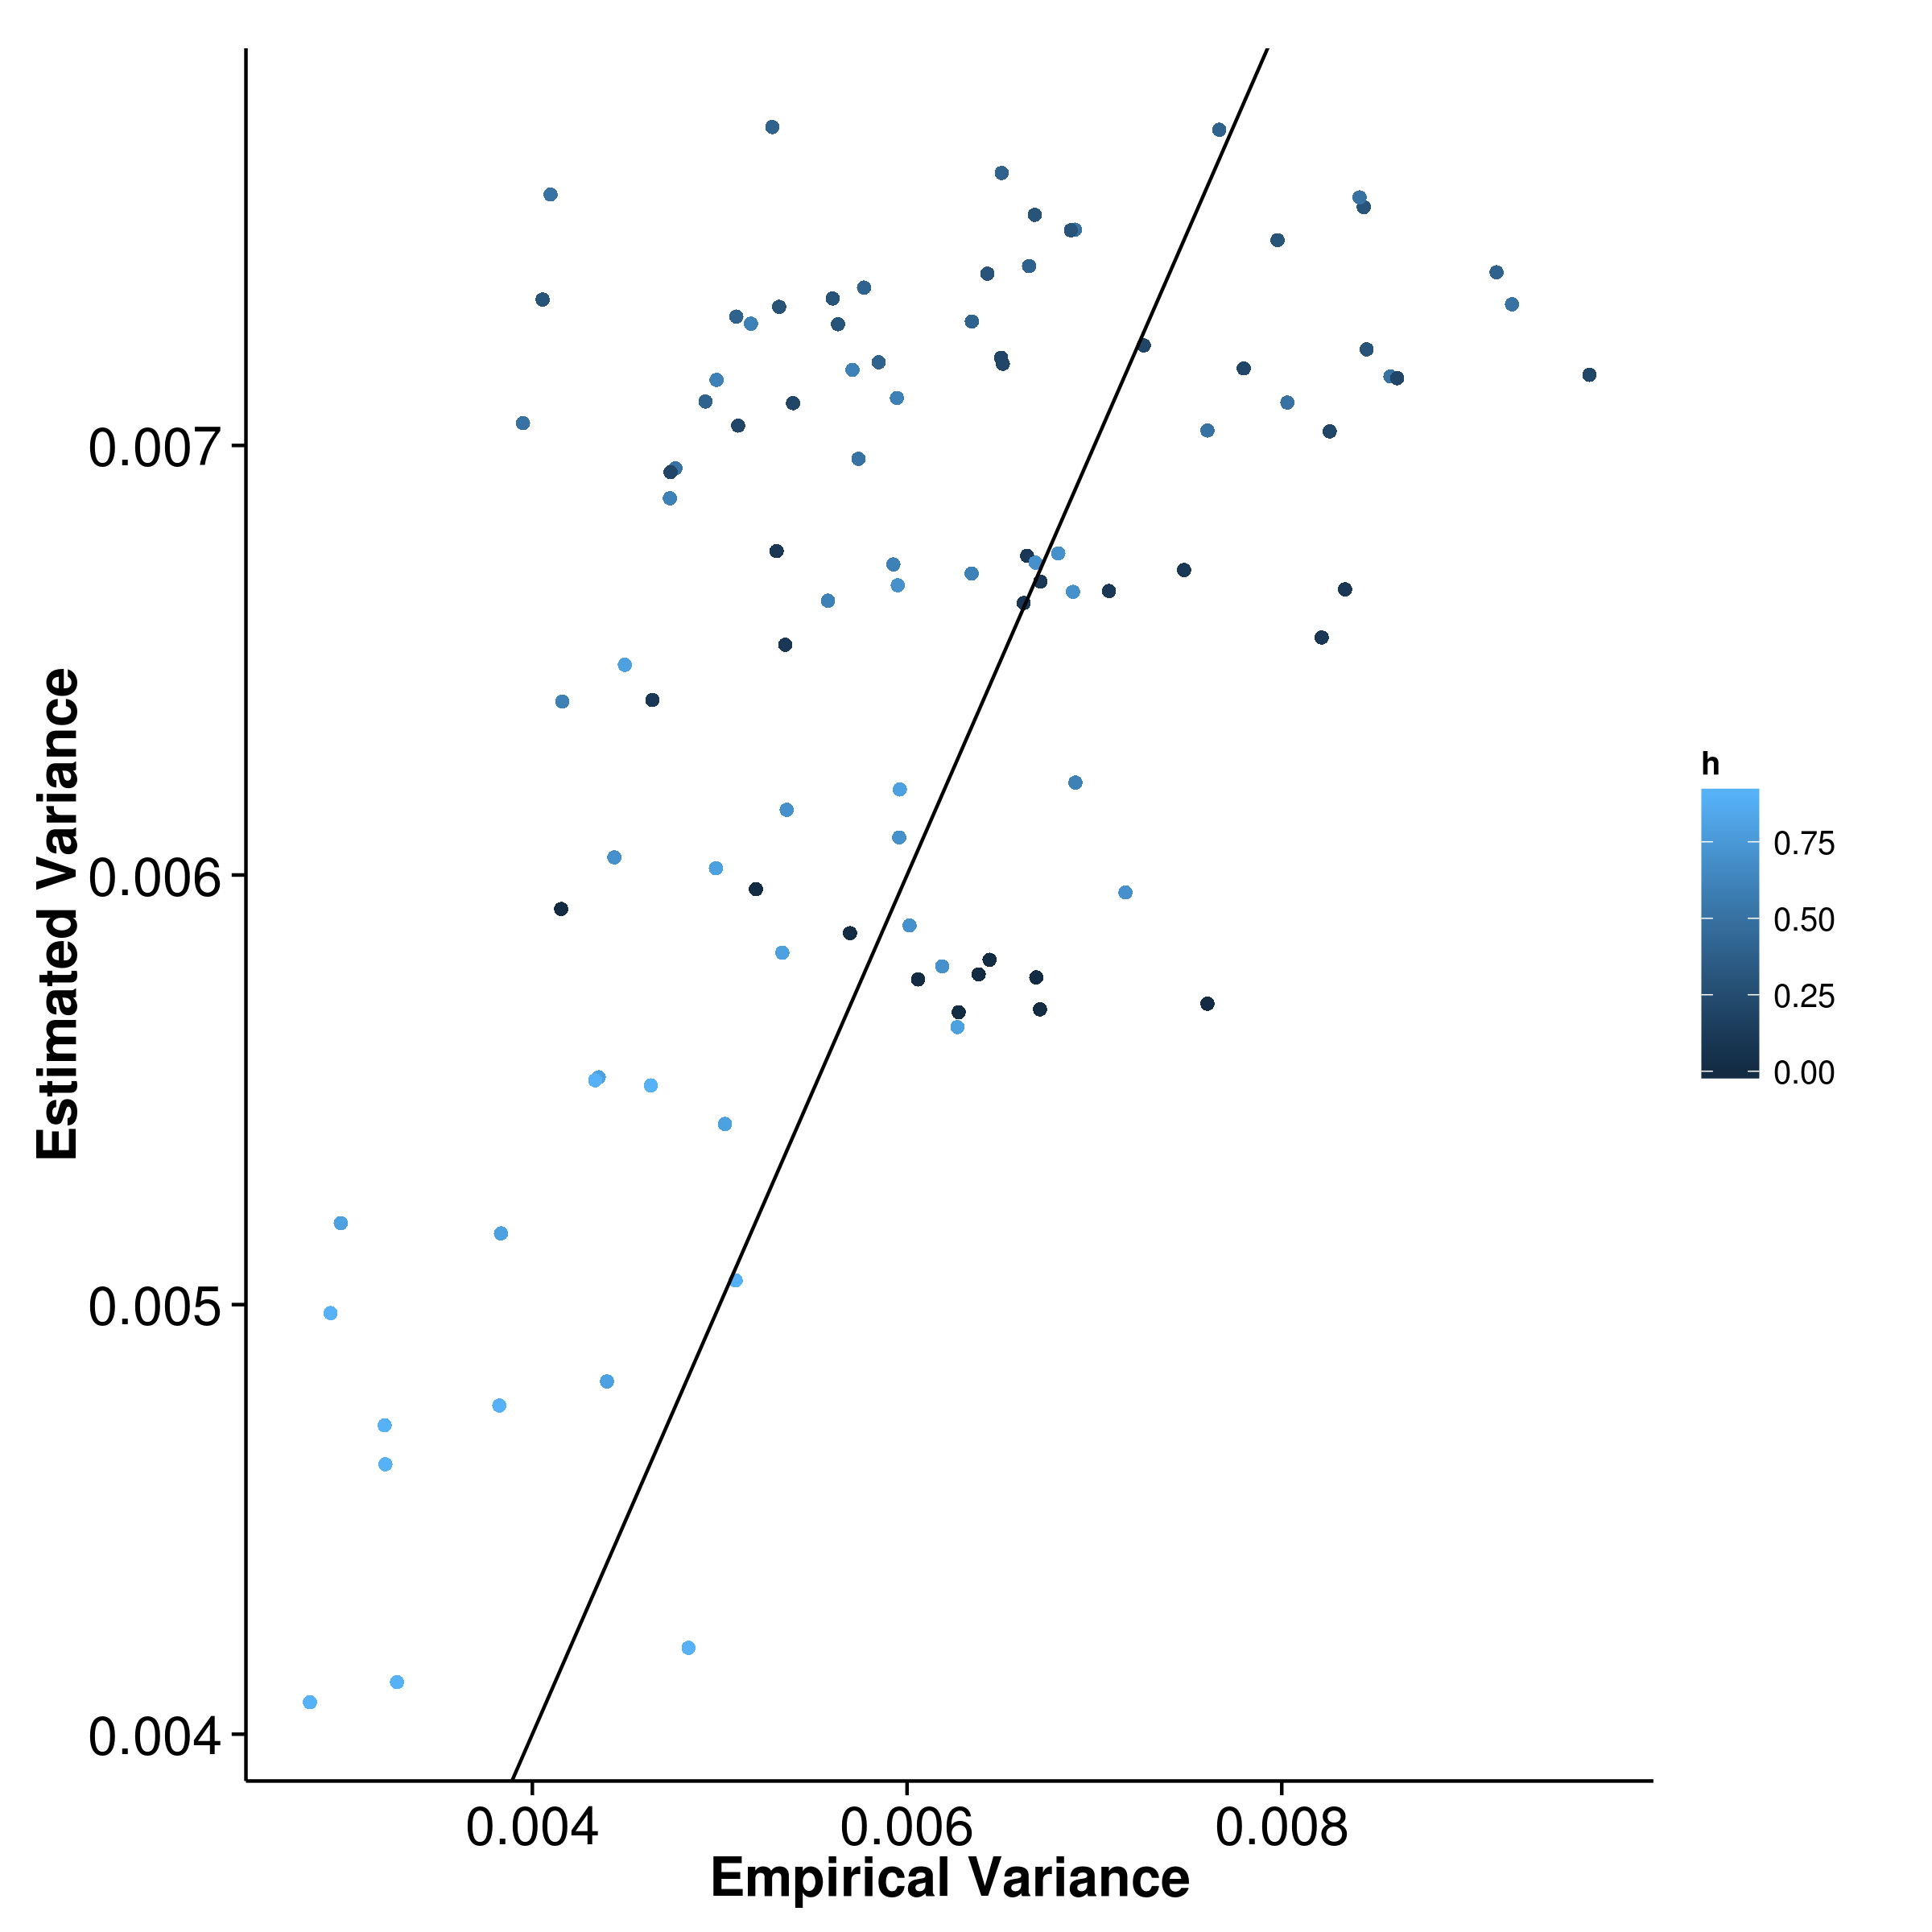
\includegraphics{figure/quantitative/same_effect/50c/gcta_50k_50c_varH.png}}
				\label{fig:50k50cQtvarG}
			}\\
			\subfloat[LDSC with fix intercept]{
				\scalebox{.4}{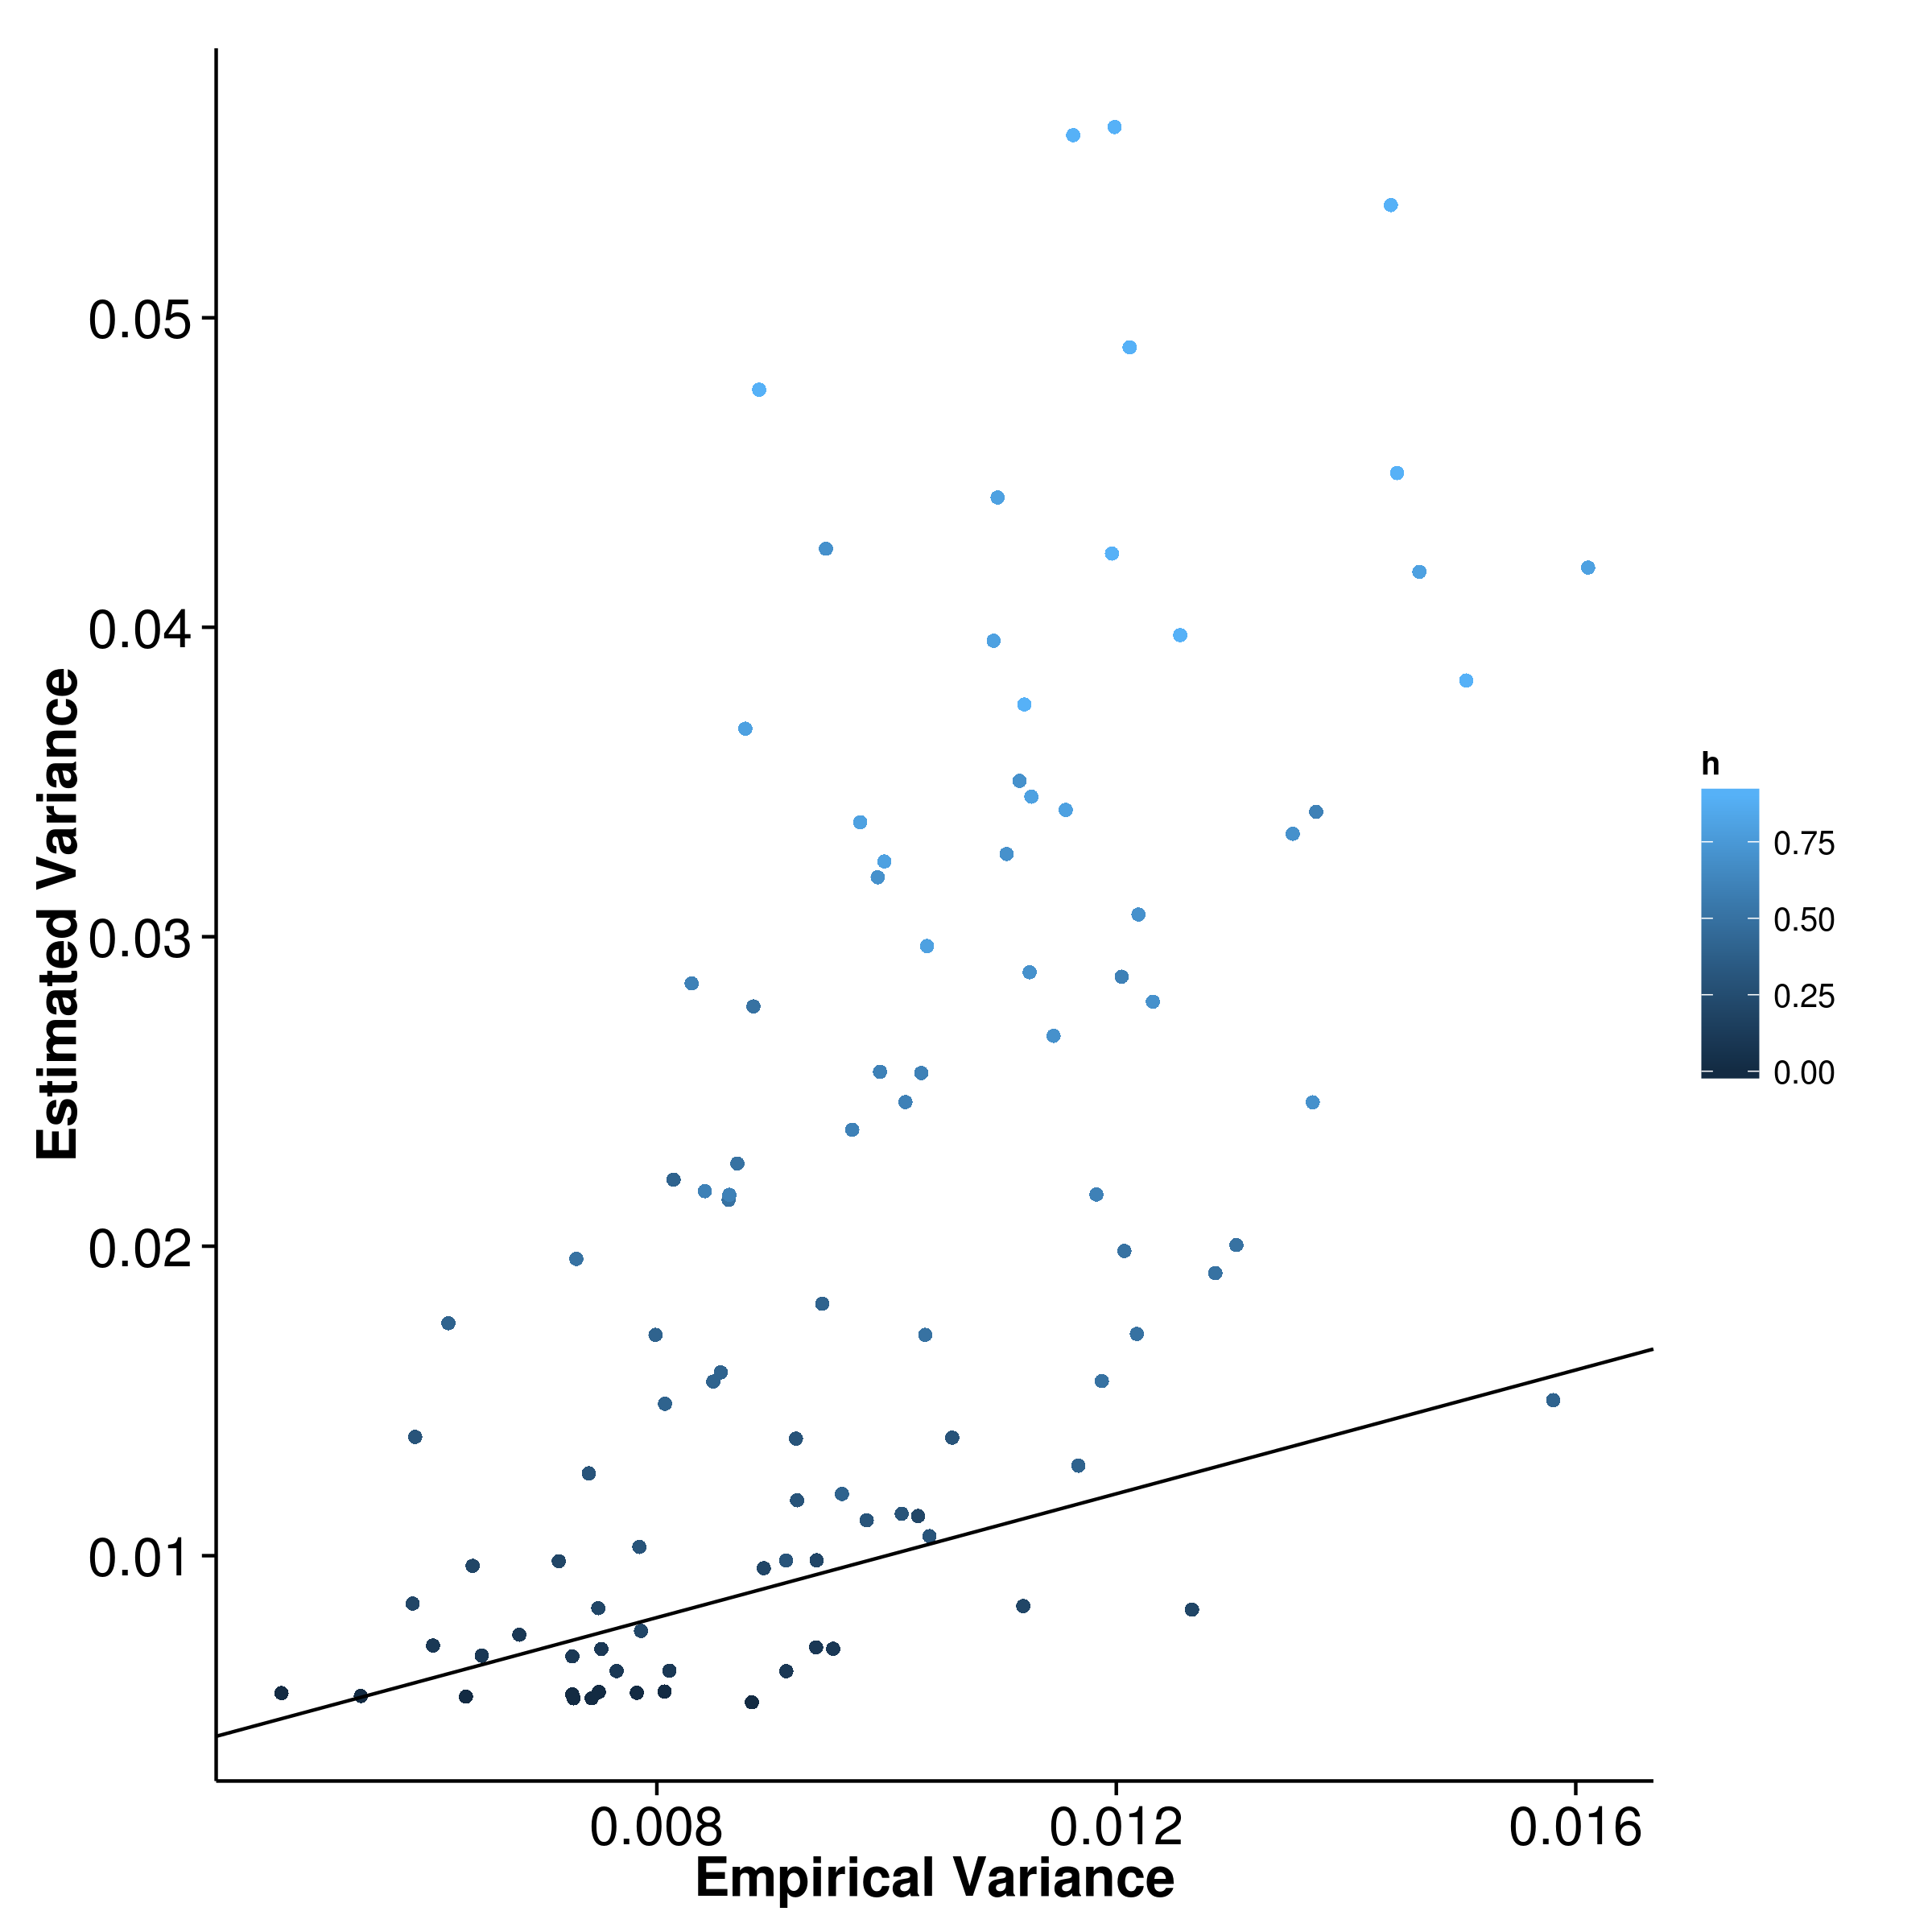
\includegraphics{figure/quantitative/same_effect/50c/ldsc_50k_50c_varH.png}}
				\label{fig:50k50cQtvarL}
			}
			\subfloat[LDSC with intercept estimation]{
				\scalebox{.4}{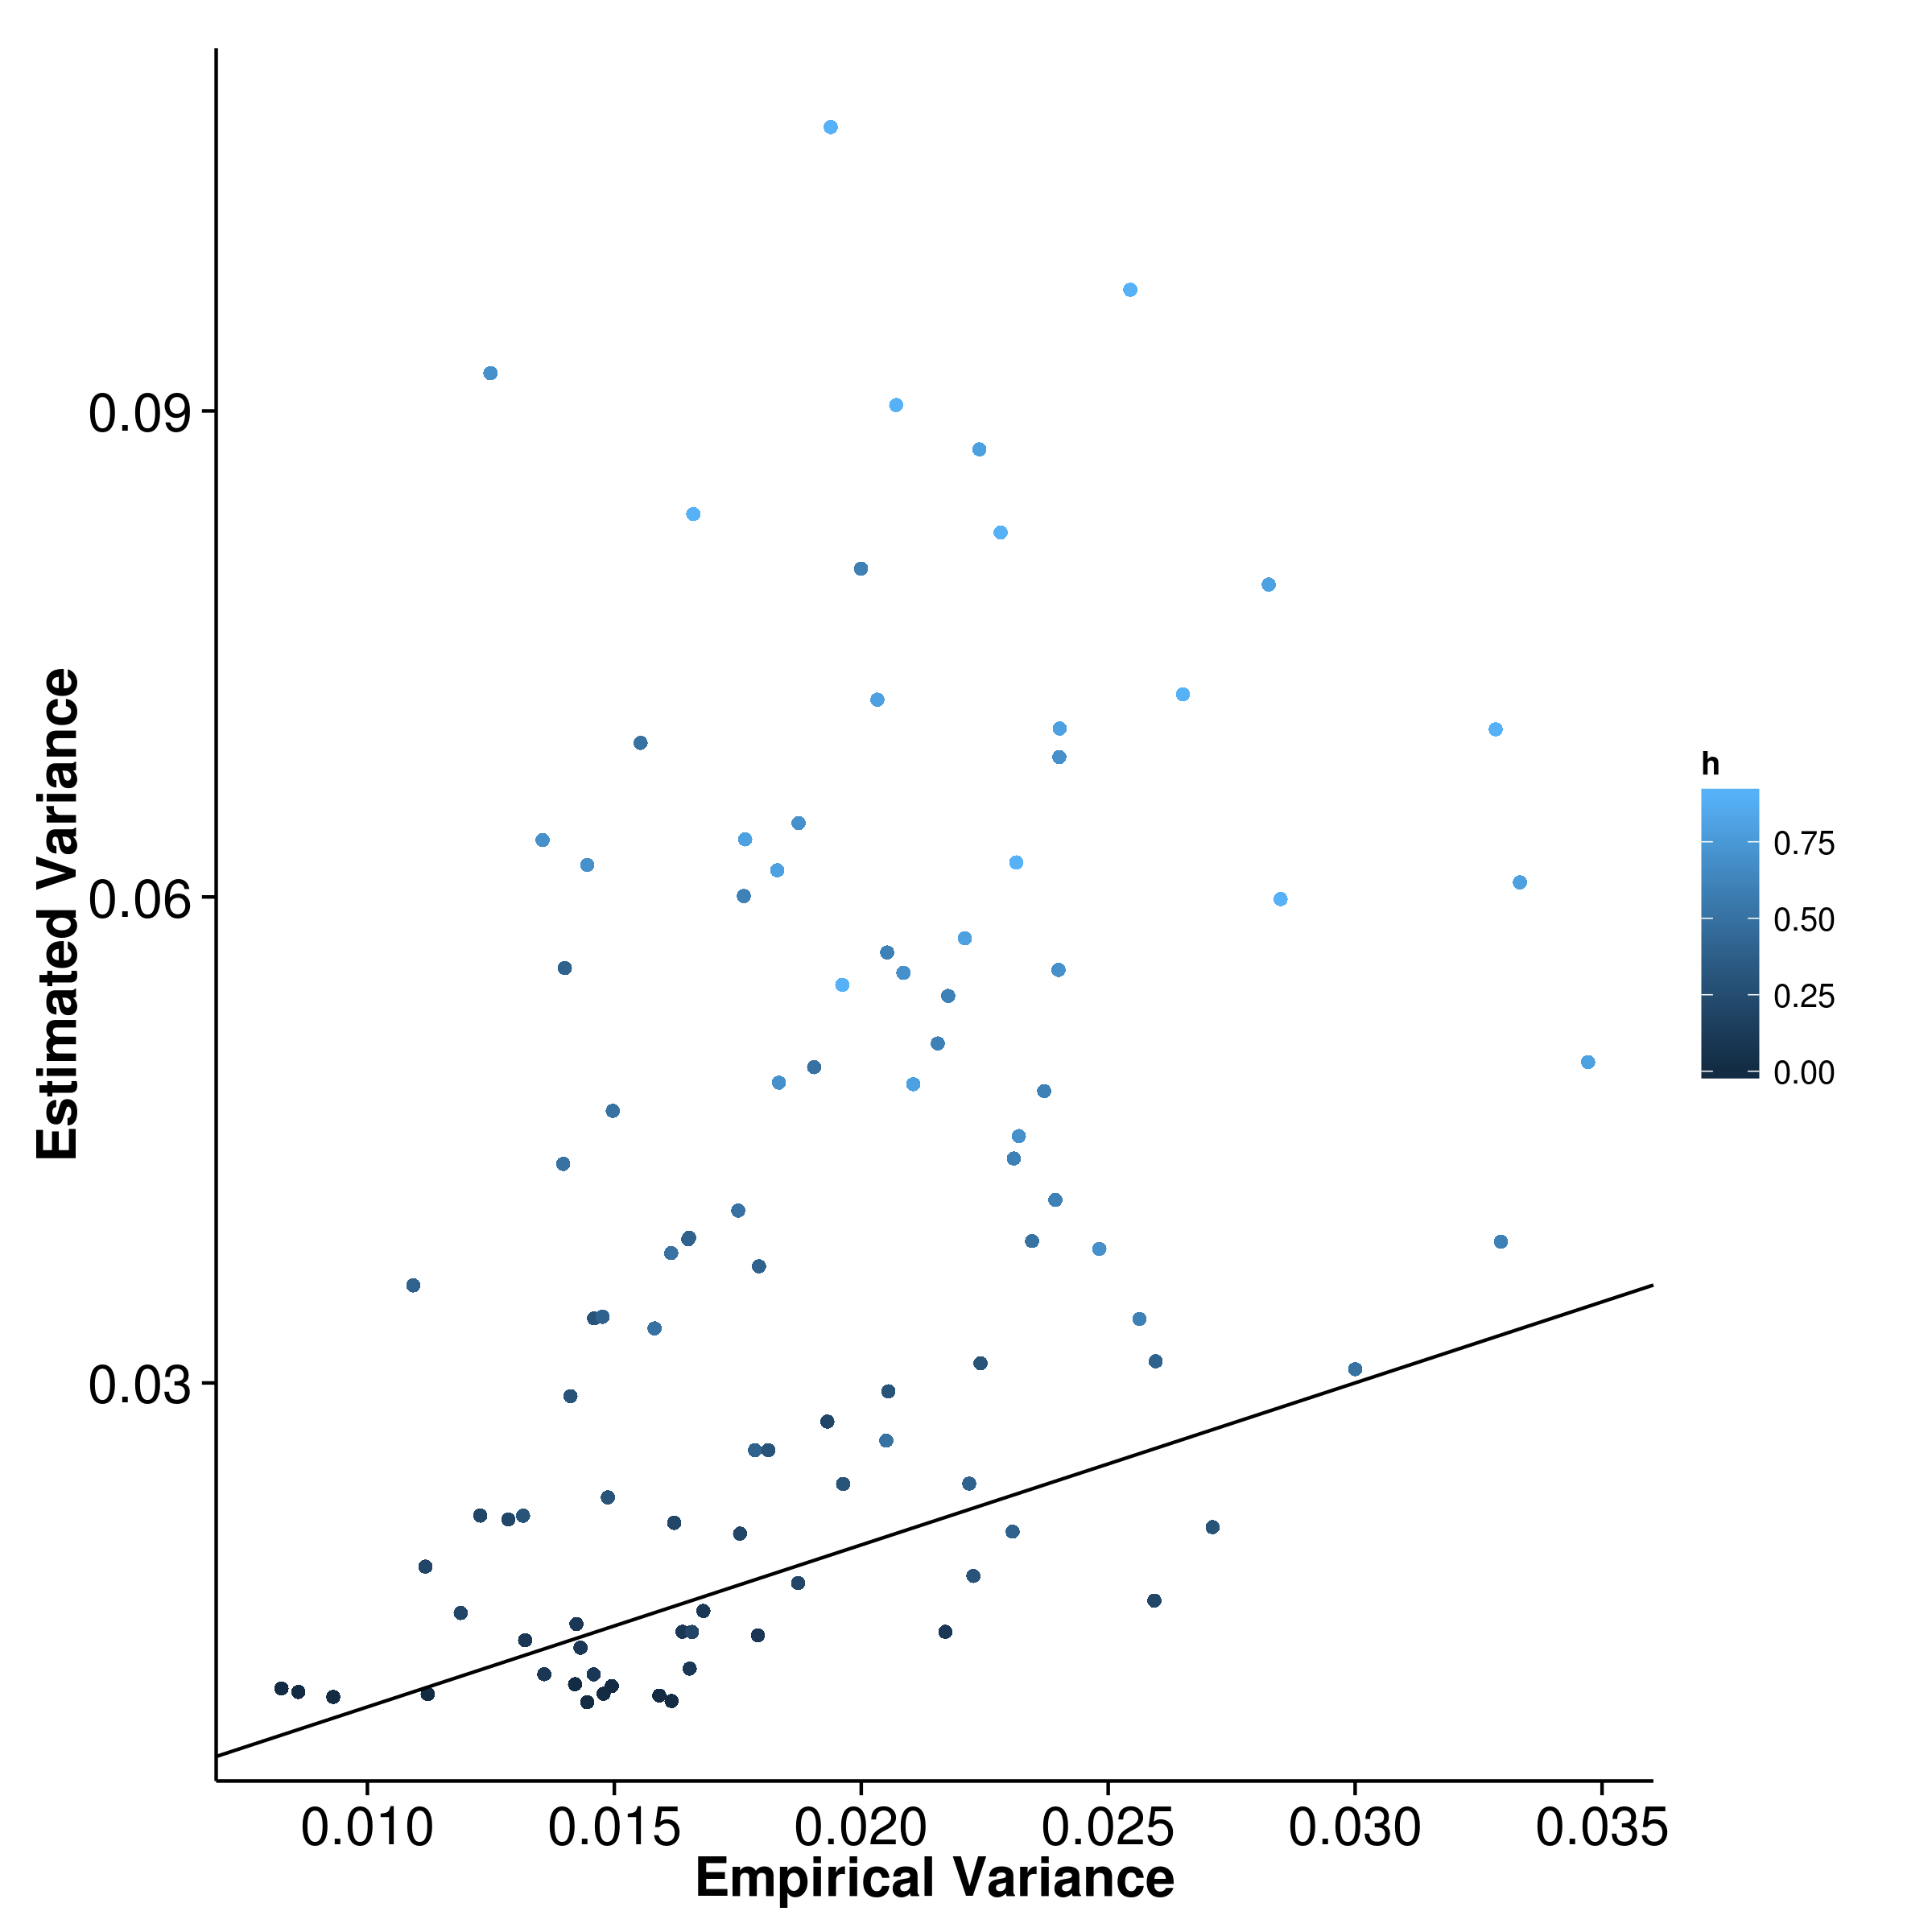
\includegraphics{figure/quantitative/same_effect/50c/ldscIn_50k_50c_varH.png}}
				\label{fig:50k50cQtvarI}
			}
			\label{fig:50k50cQtVar}
		\end{figure}
		
		
		\begin{figure}
			\centering
			\centering
			\subfloat[SHREK]{
				\scalebox{.4}{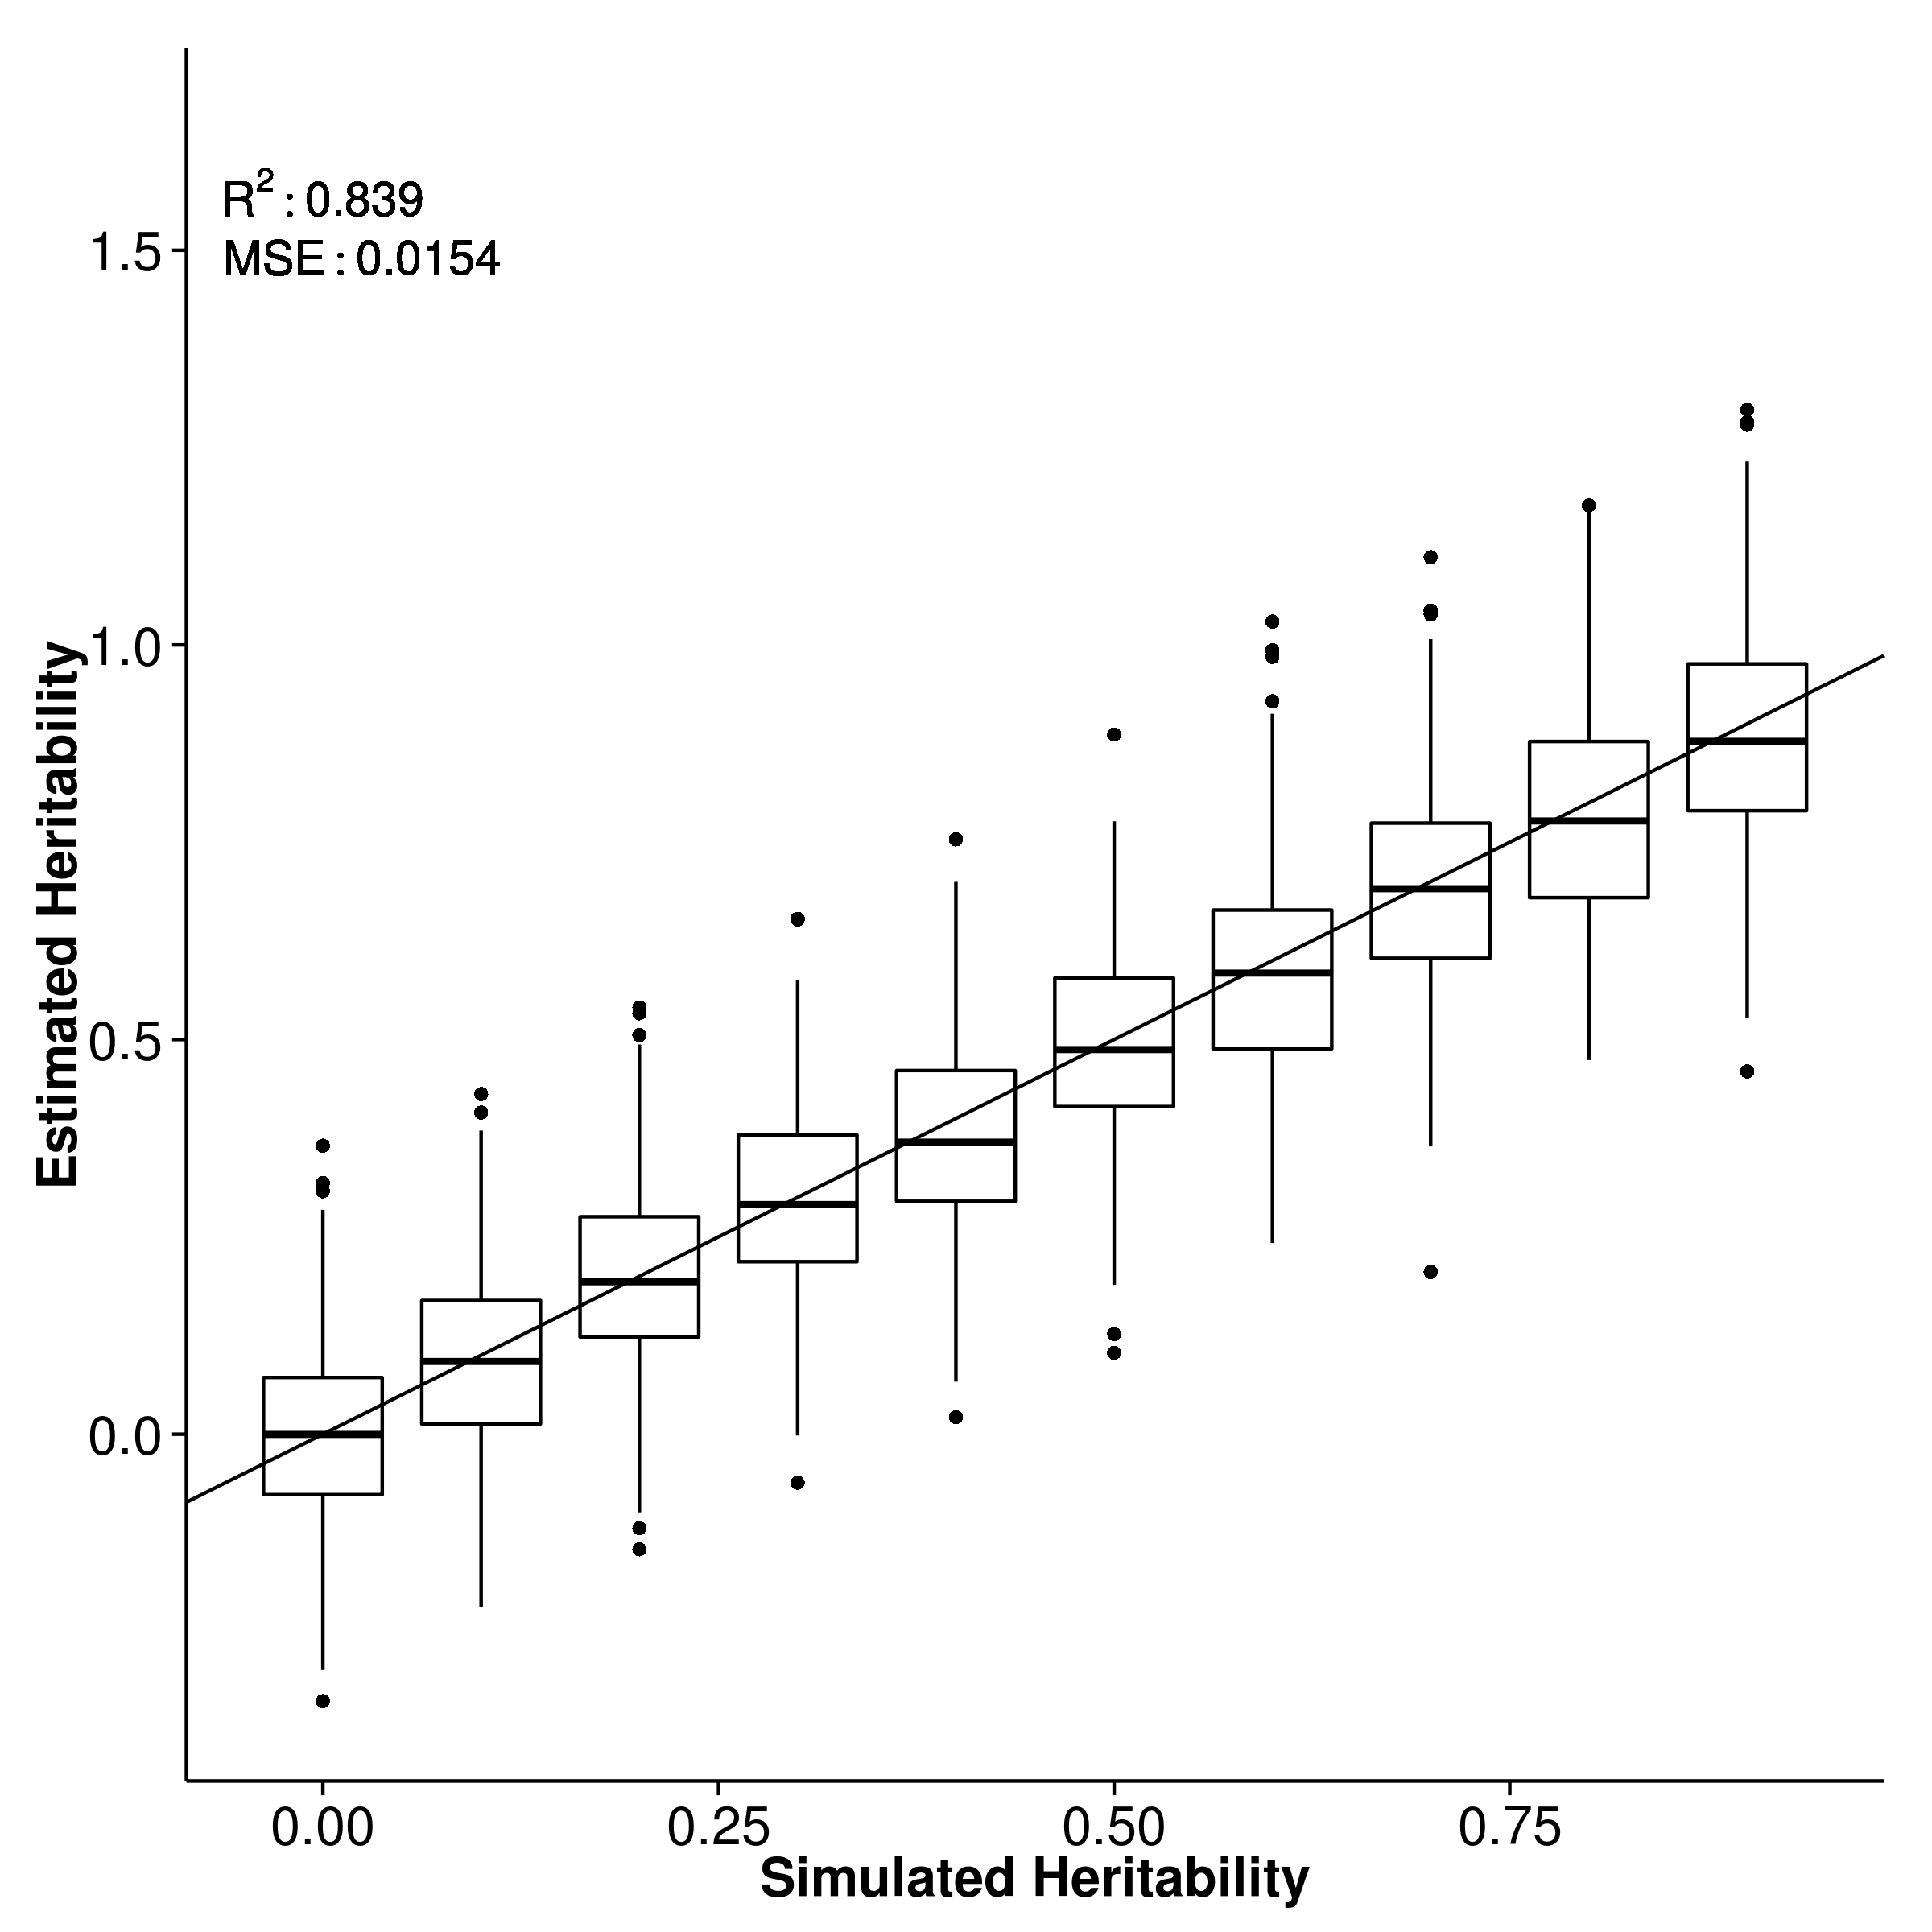
\includegraphics{figure/quantitative/same_effect/100c/shrek_50k_100c_meanH.png}}
				\label{fig:50k100cQtmeanS}
			}
			\subfloat[GCTA]{
				\scalebox{.4}{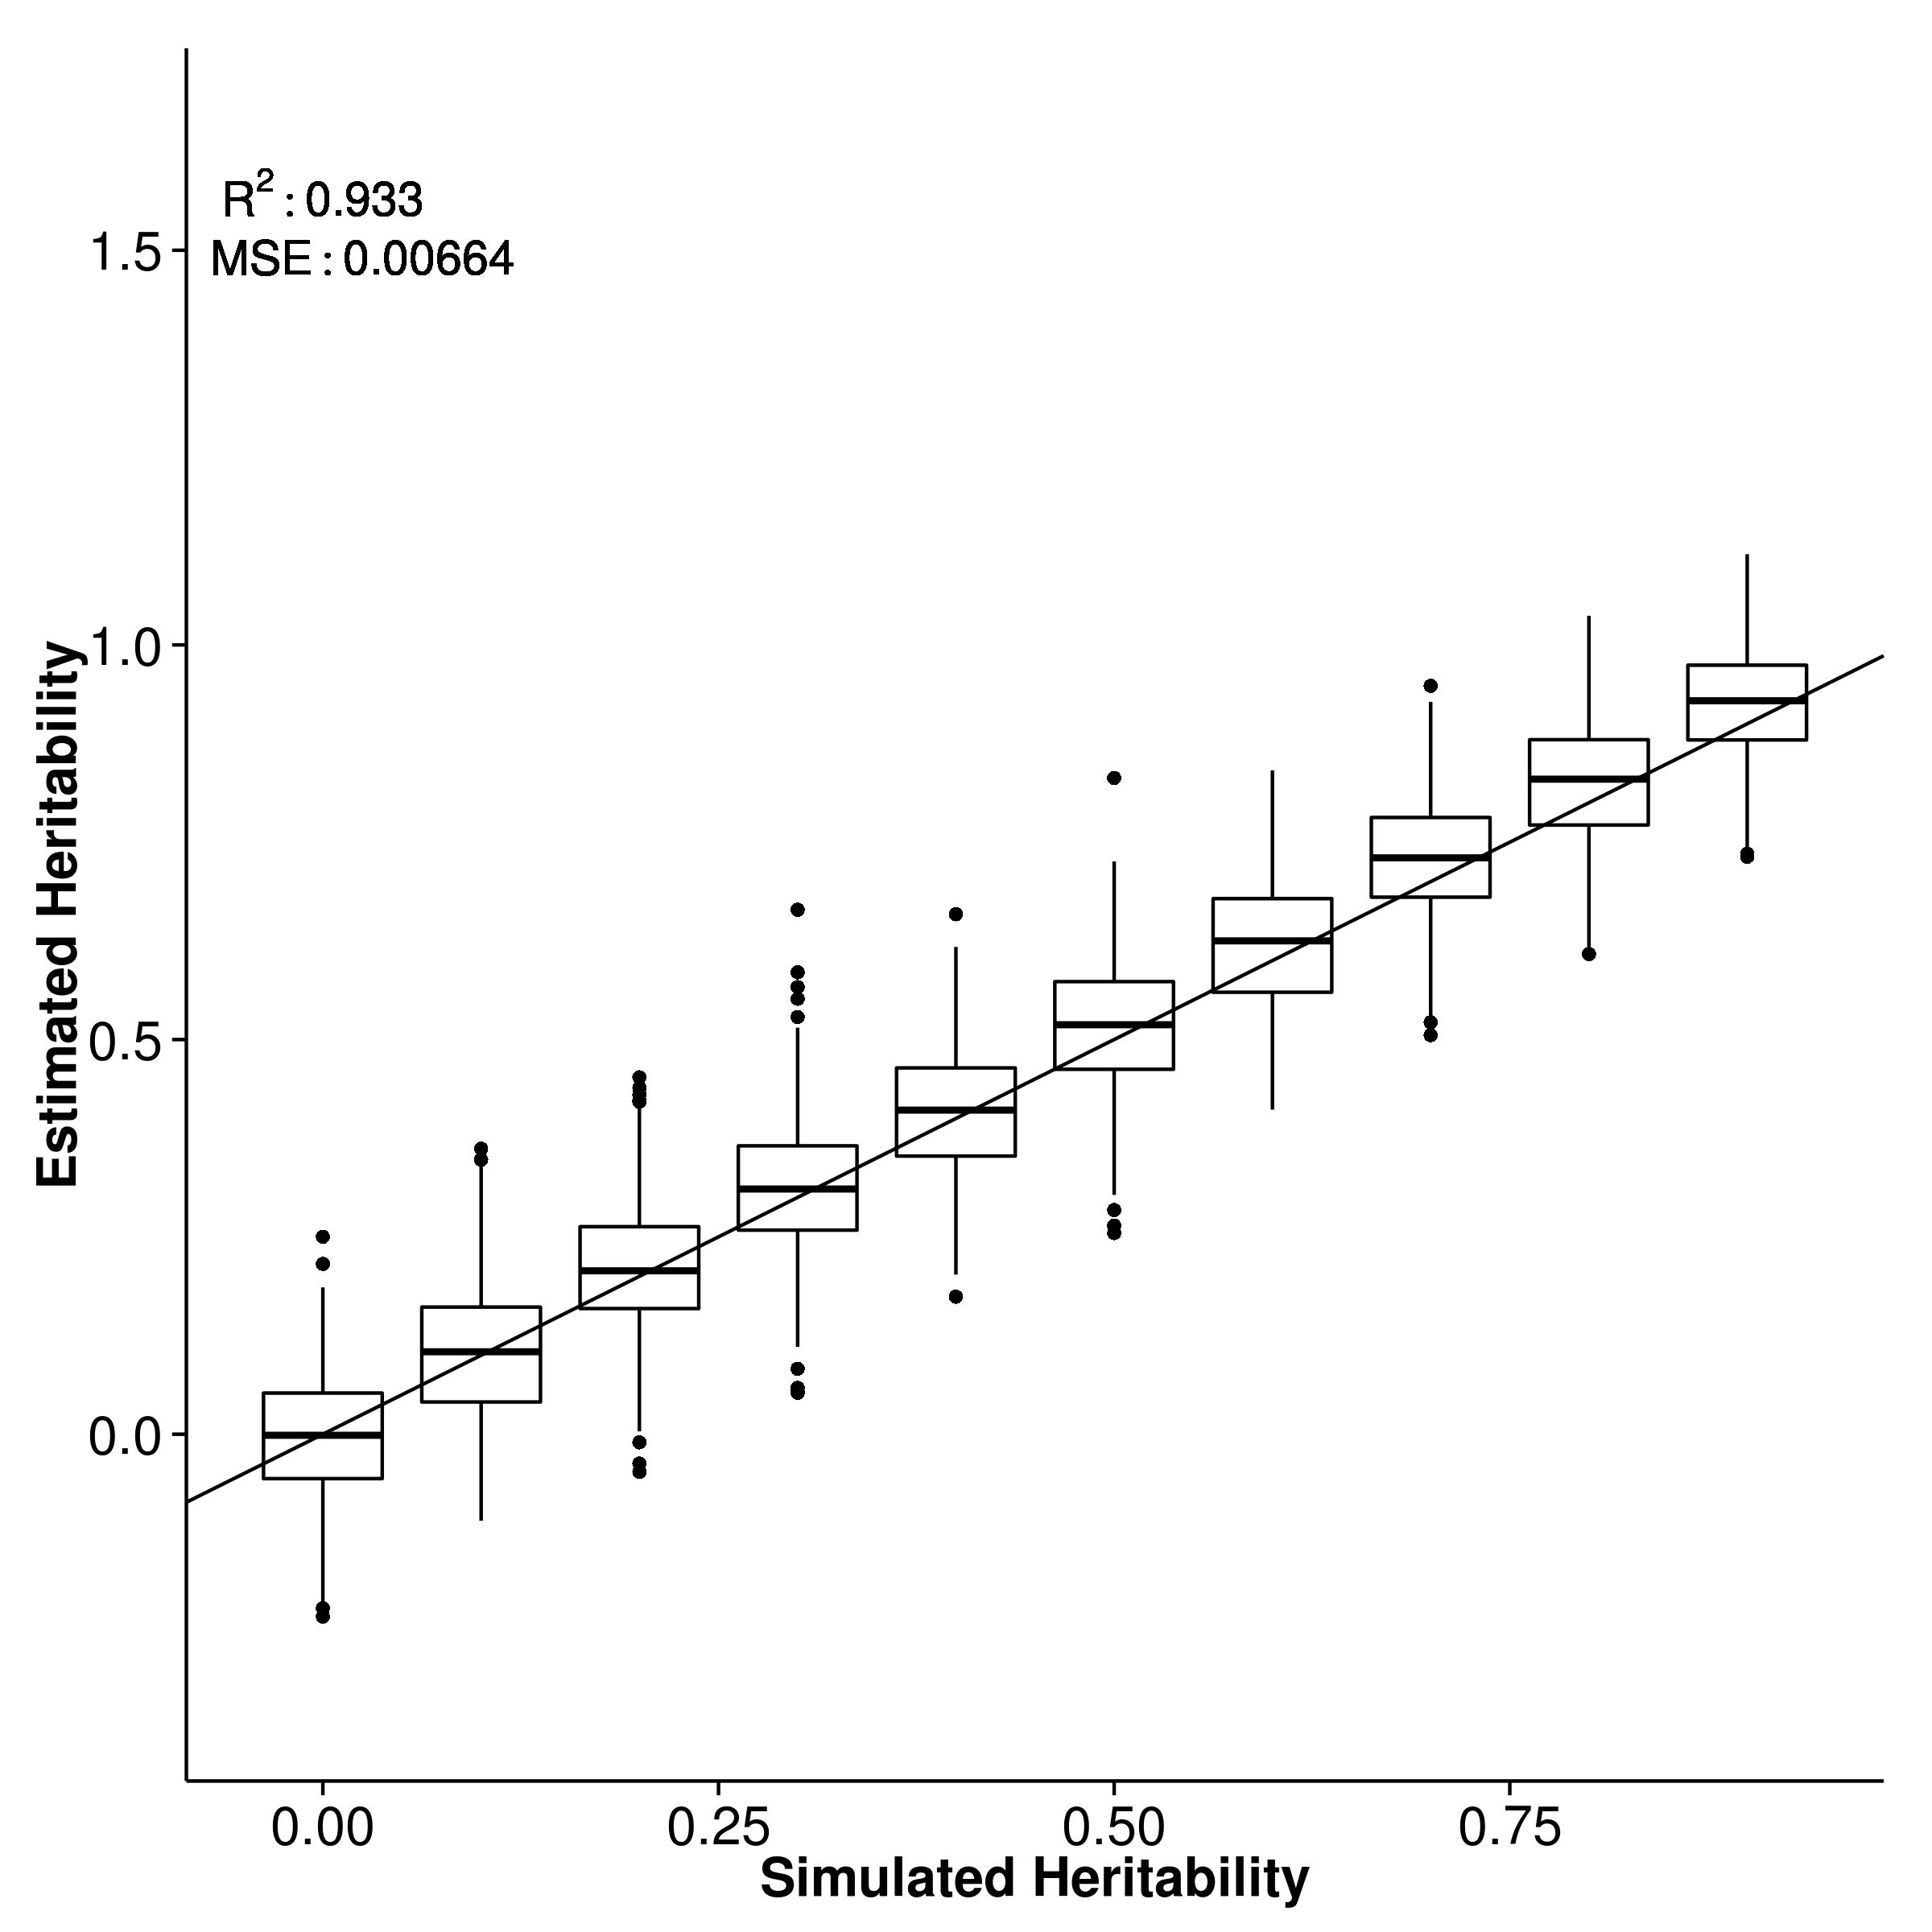
\includegraphics{figure/quantitative/same_effect/100c/gcta_50k_100c_meanH.png}}
				\label{fig:50k100cQtmeanG}
			}\\
			\subfloat[LDSC with fix intercept]{
				\scalebox{.4}{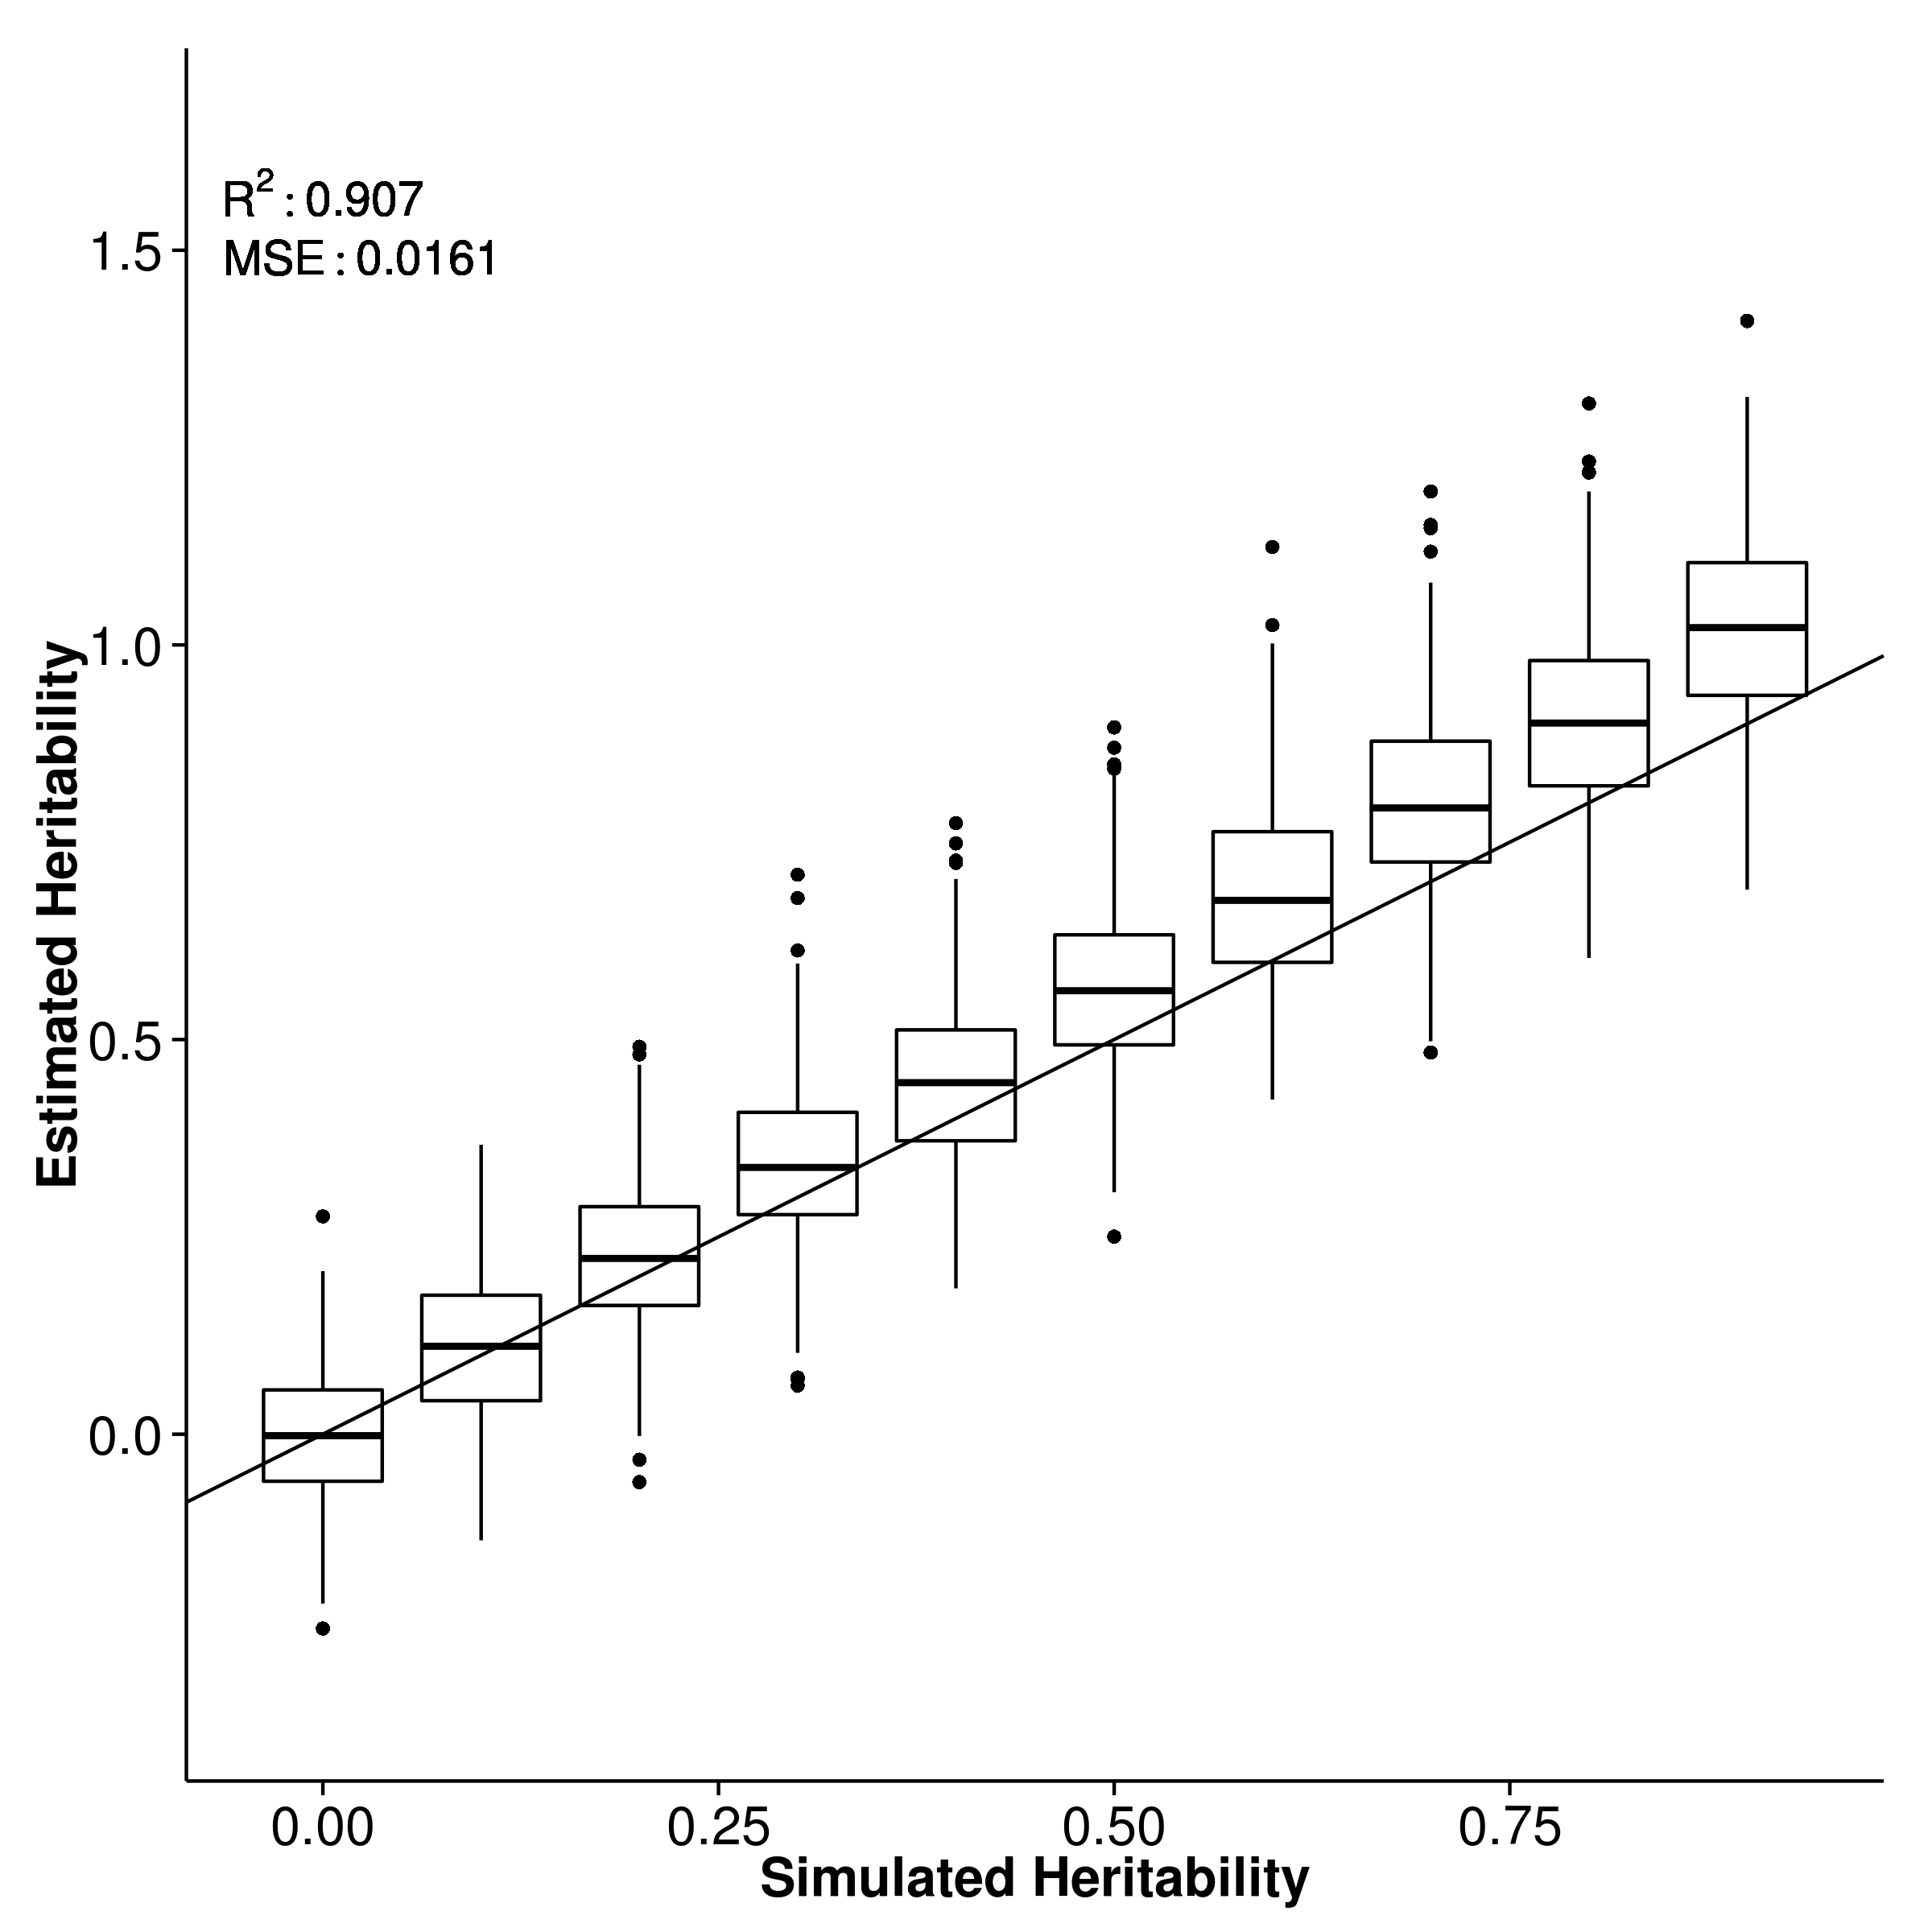
\includegraphics{figure/quantitative/same_effect/100c/ldsc_50k_100c_meanH.png}}
				\label{fig:50k100cQtmeanL}
			}
			\subfloat[LDSC with intercept estimation]{
				\scalebox{.4}{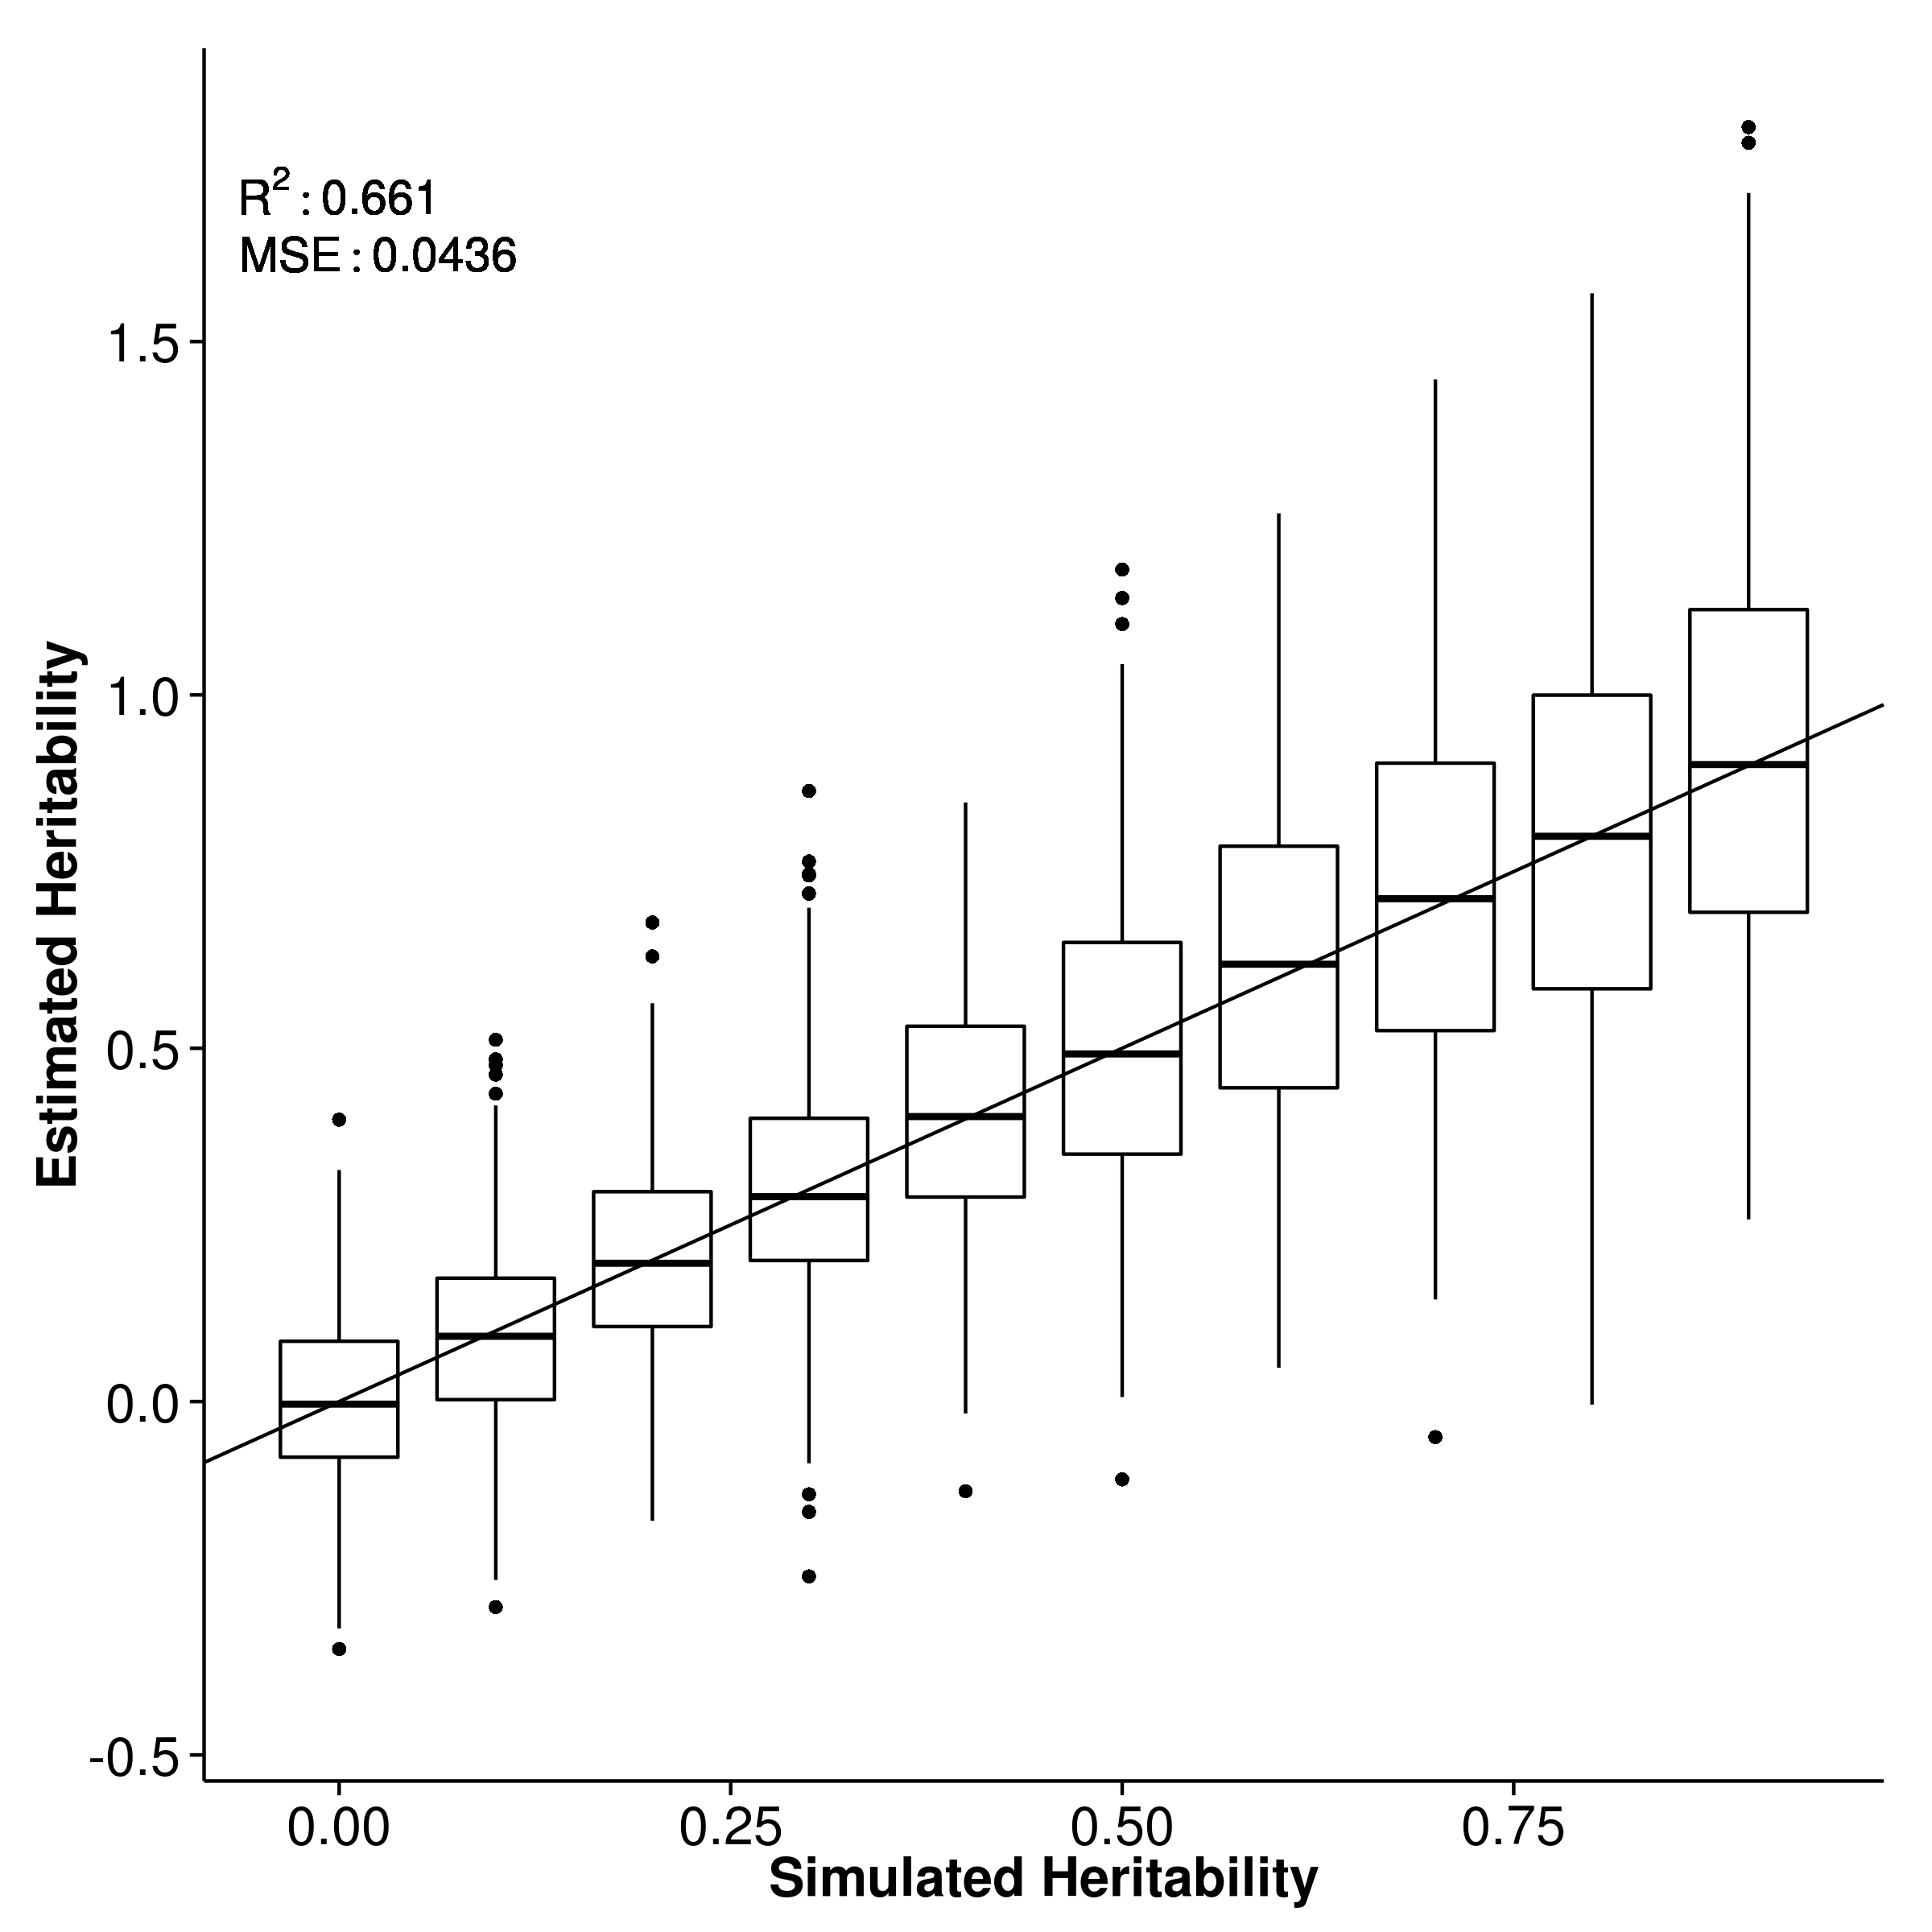
\includegraphics{figure/quantitative/same_effect/100c/ldscIn_50k_100c_meanH.png}}
				\label{fig:50k100cQtmeanI}
			}
			\caption[Simulation of Quantitative Traits with 50k \glsentryshortpl{SNP} and 100 causal variants of same effect size]
			{Simulation of Quantitative Traits with 50k \glsentryshortpl{SNP} and 100 causal variants with same effect size.} 
			\label{fig:50k100cQtMean}
		\end{figure}
		\begin{figure}
			\centering
			\centering
			\subfloat[SHREK]{
				\scalebox{.4}{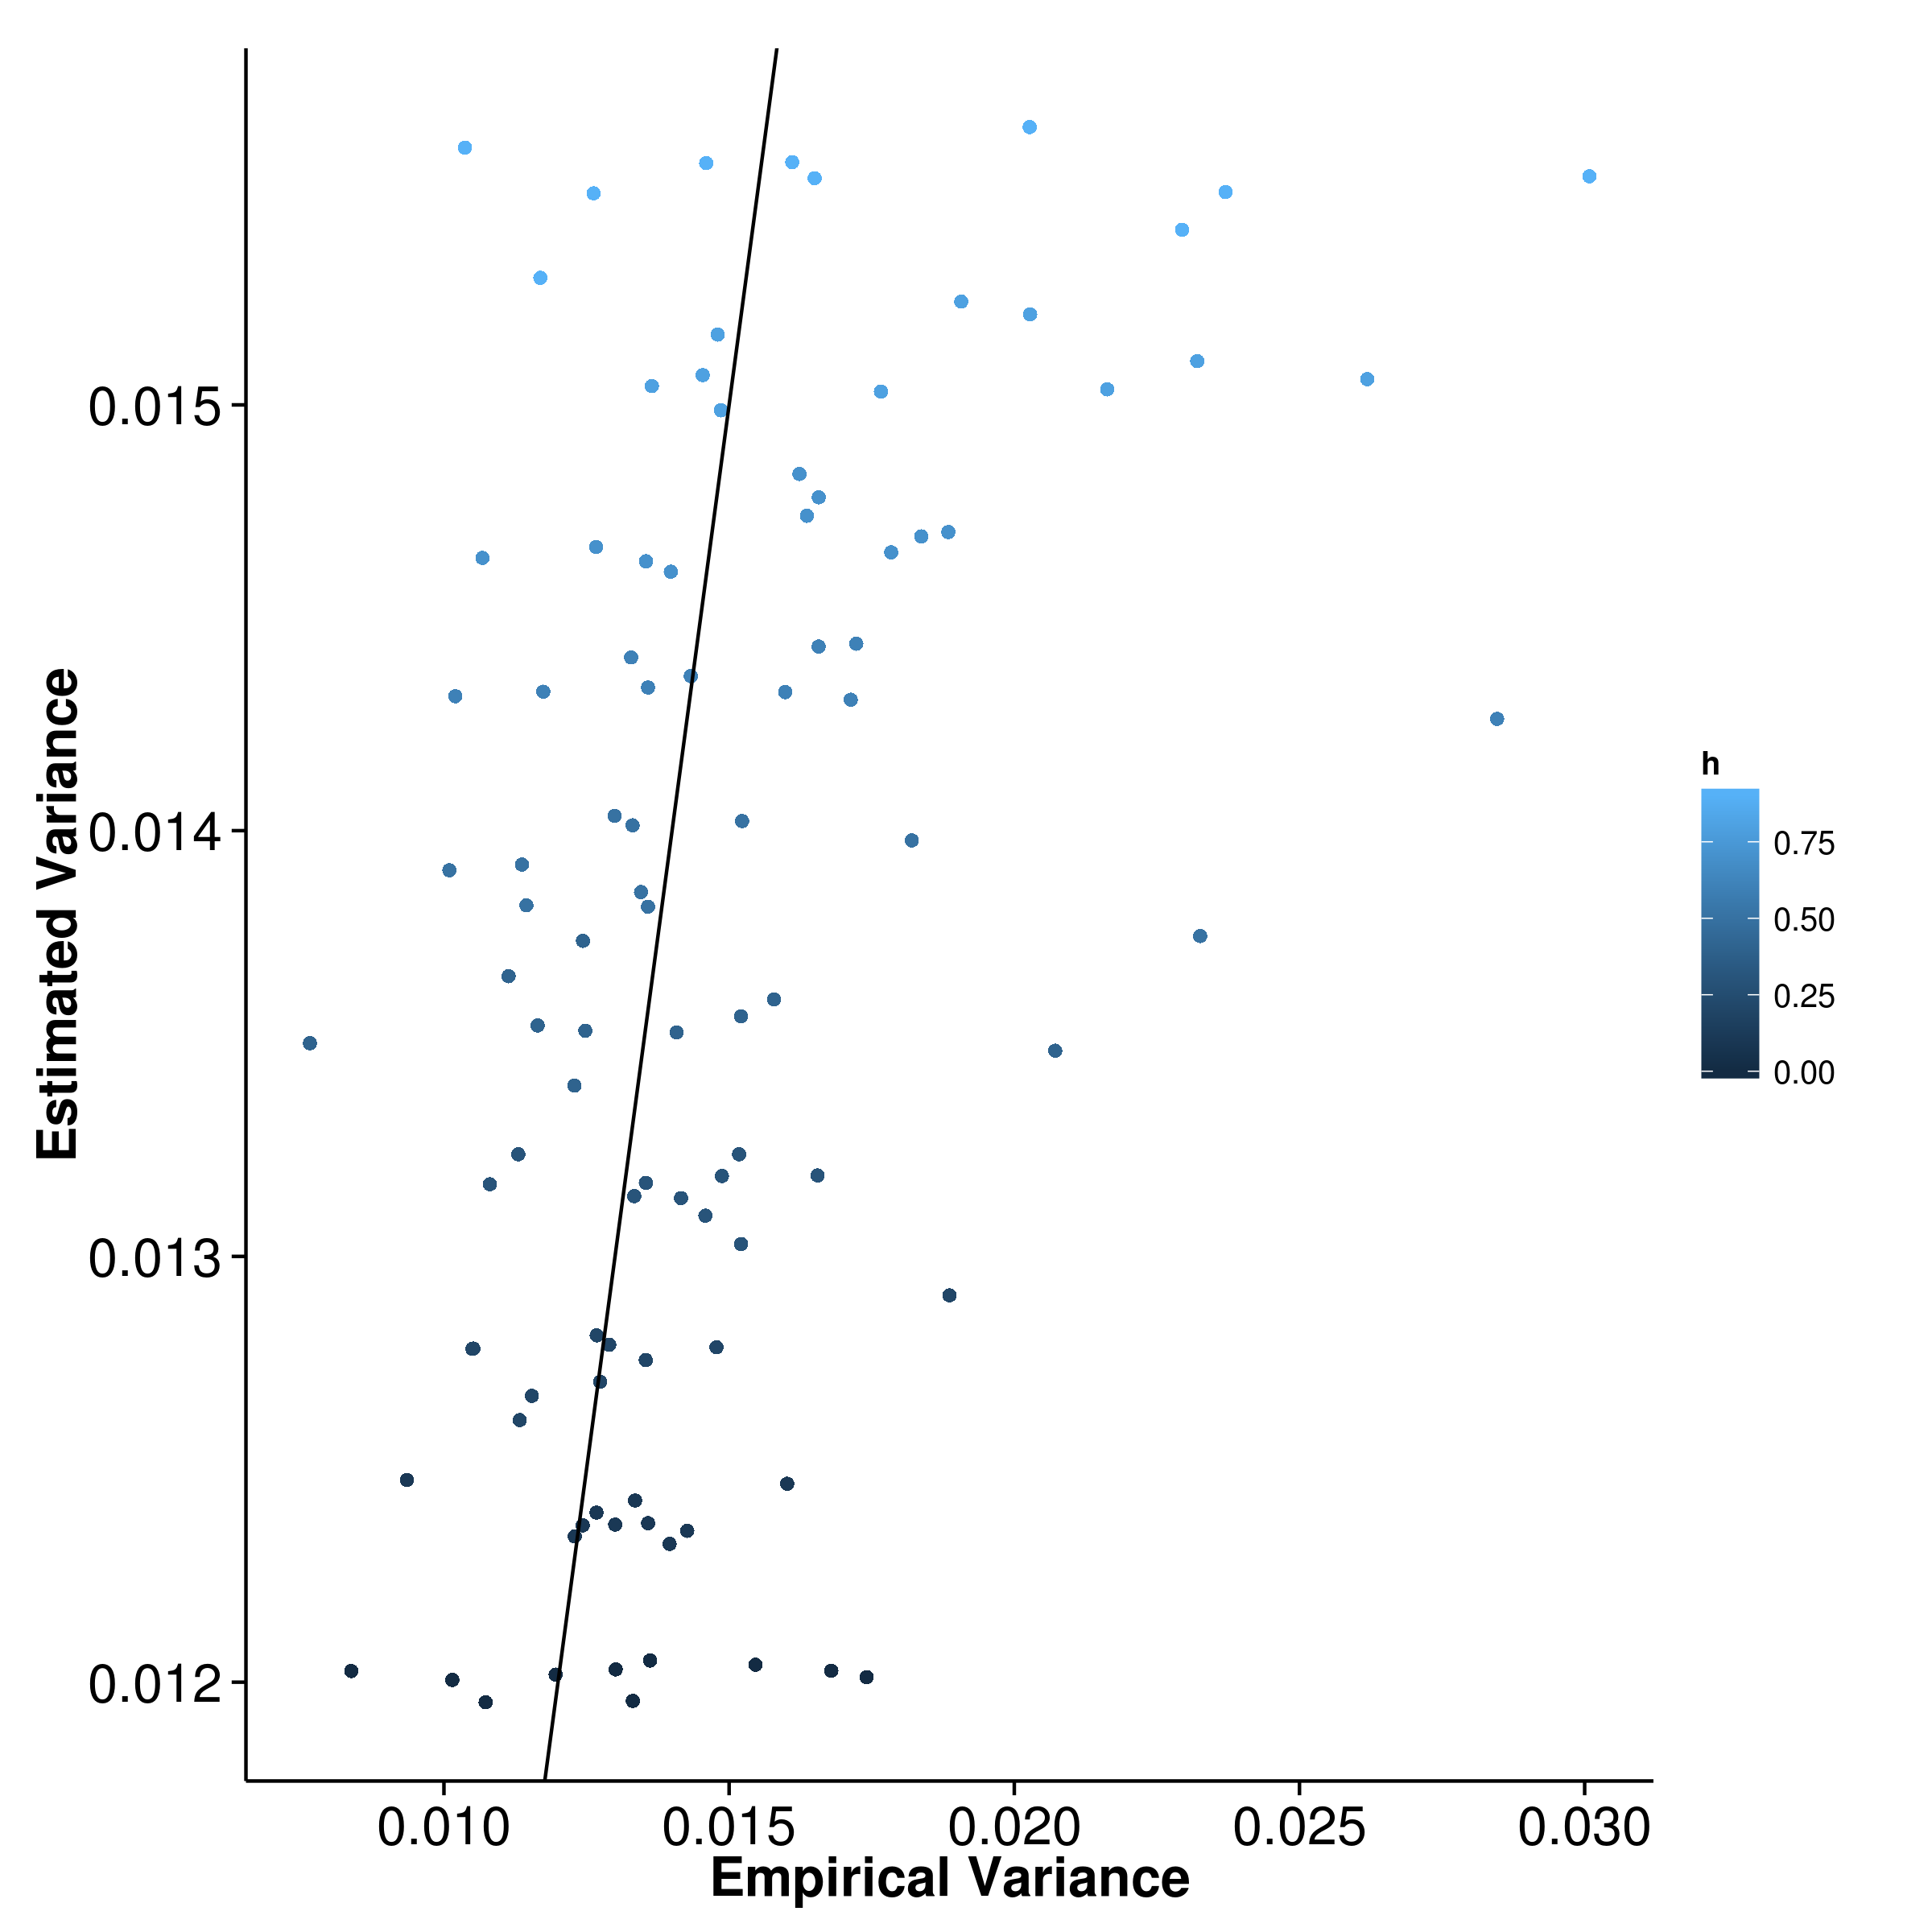
\includegraphics{figure/quantitative/same_effect/100c/shrek_50k_100c_varH.png}}
				\label{fig:50k100cQtvarS}
			}
			\subfloat[GCTA]{
				\scalebox{.4}{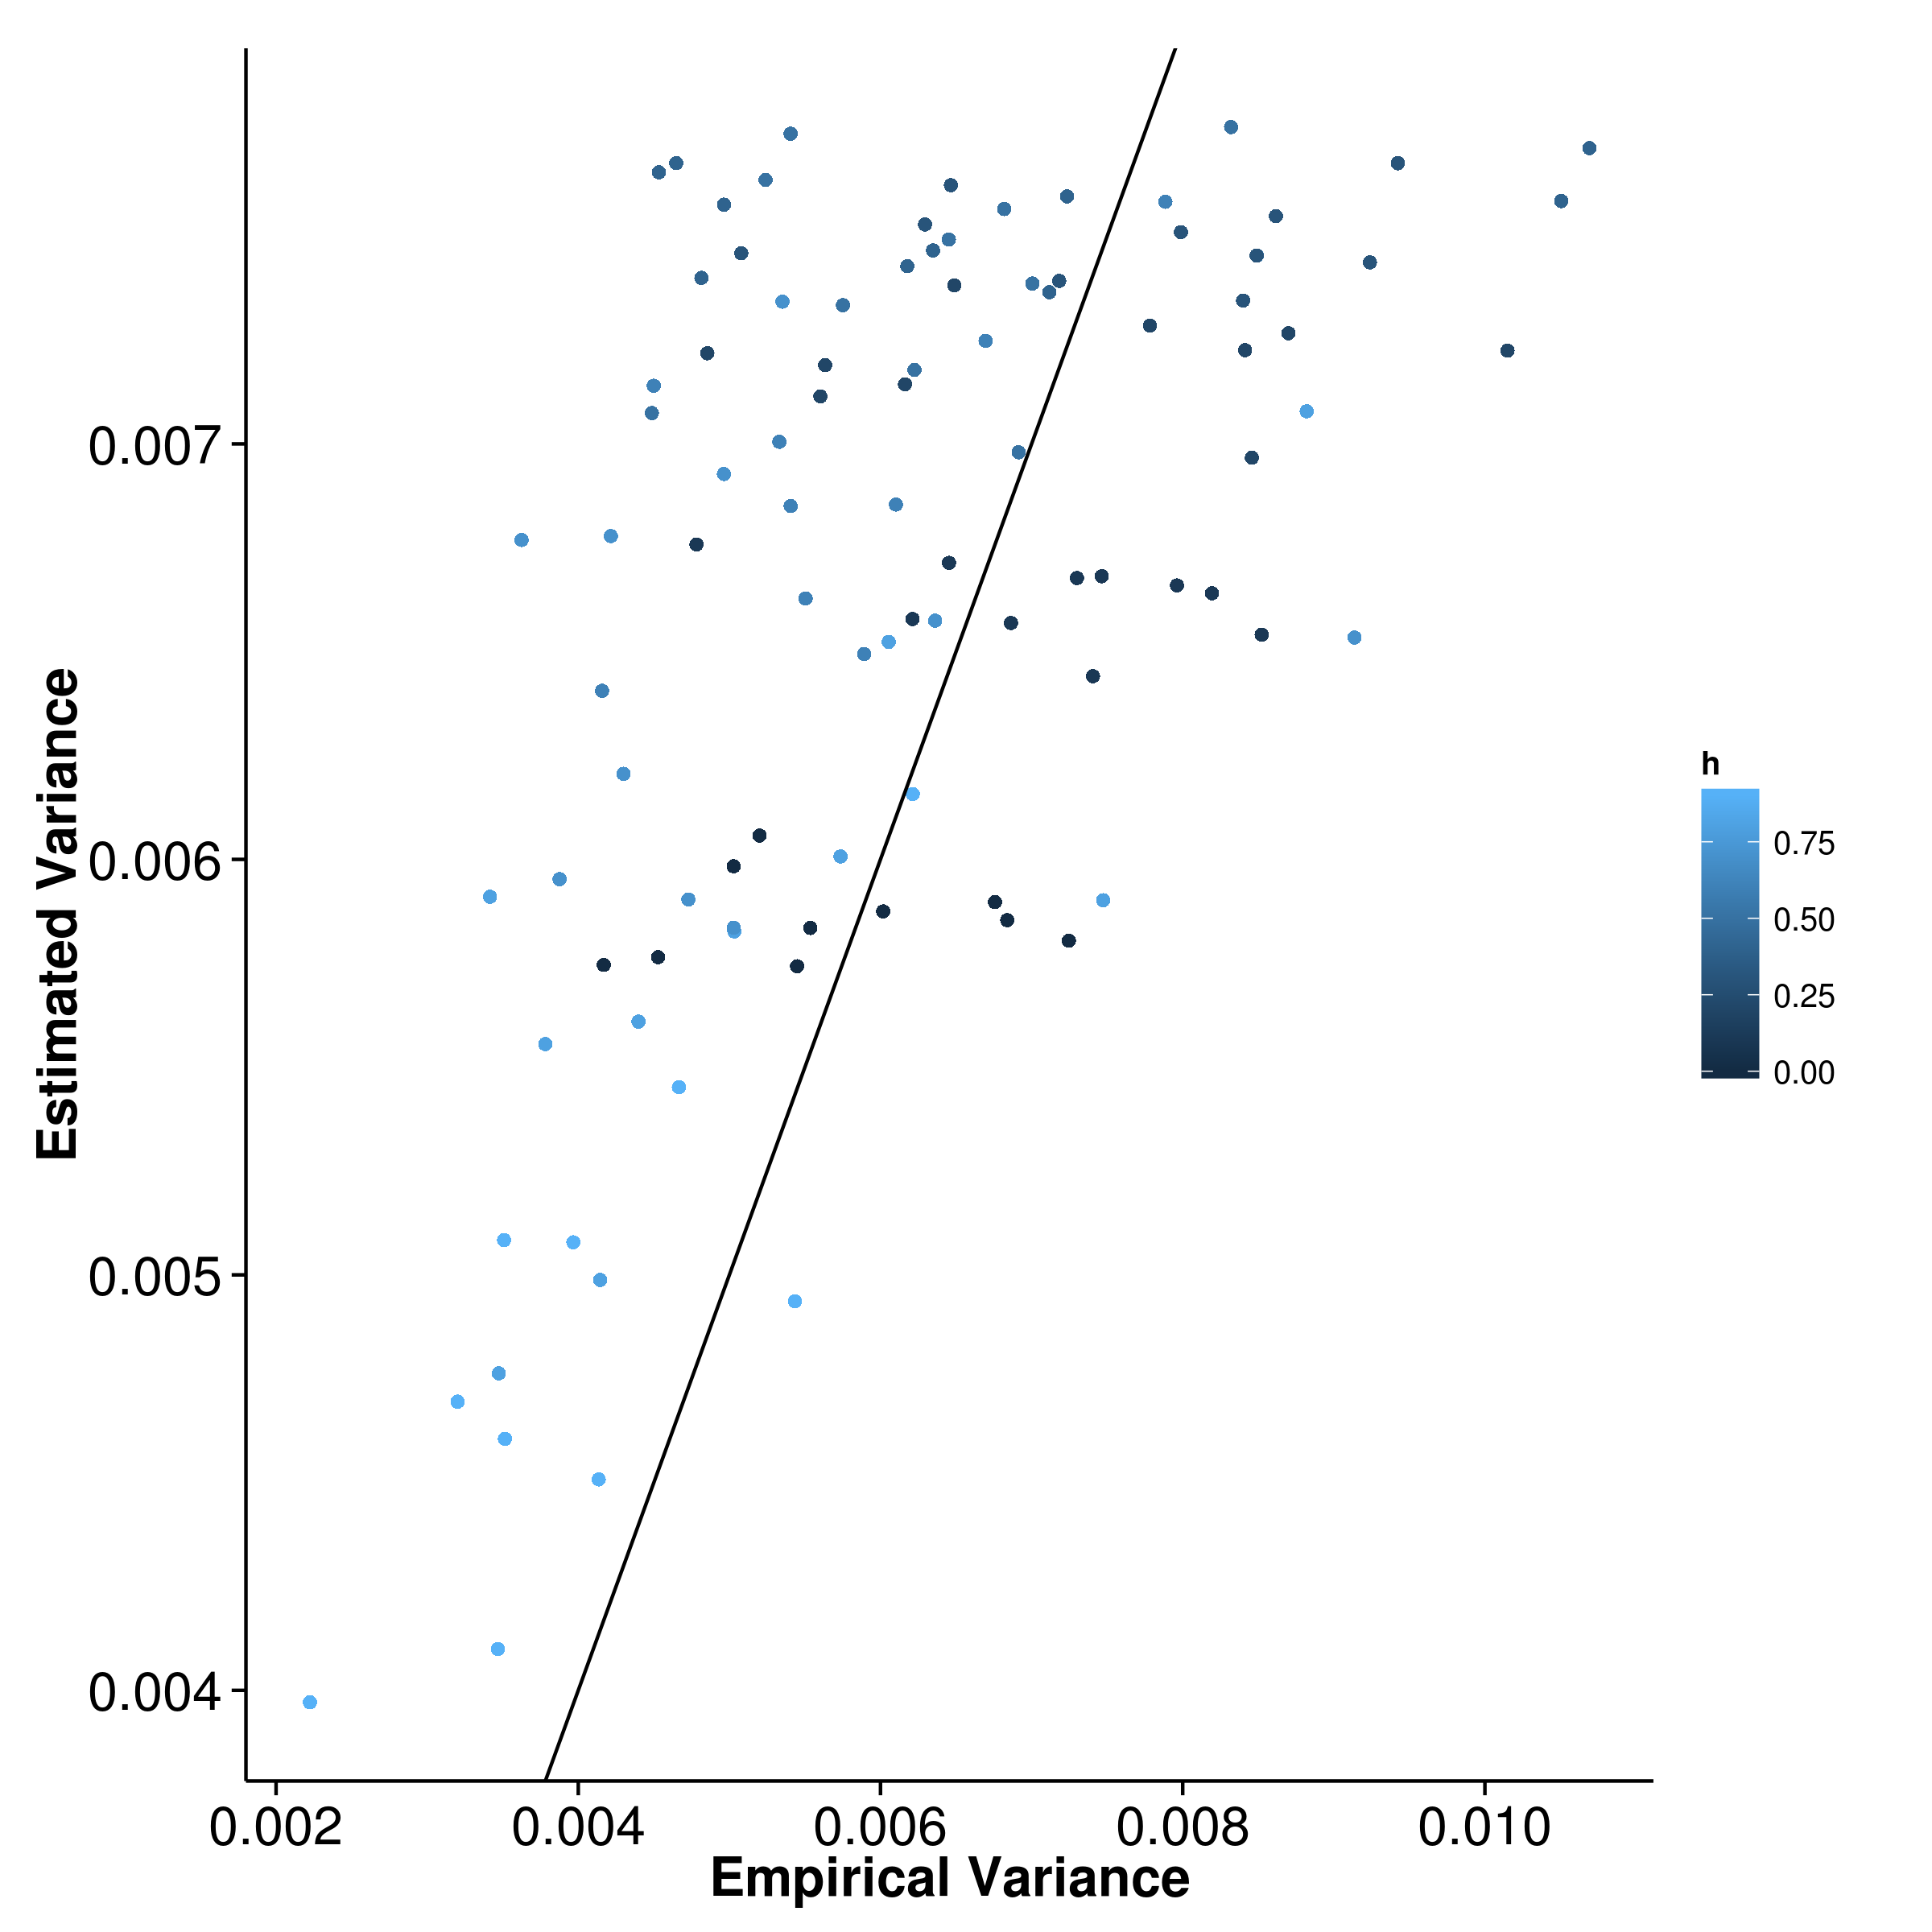
\includegraphics{figure/quantitative/same_effect/100c/gcta_50k_100c_varH.png}}
				\label{fig:50k100cQtvarG}
			}\\
			\subfloat[LDSC with fix intercept]{
				\scalebox{.4}{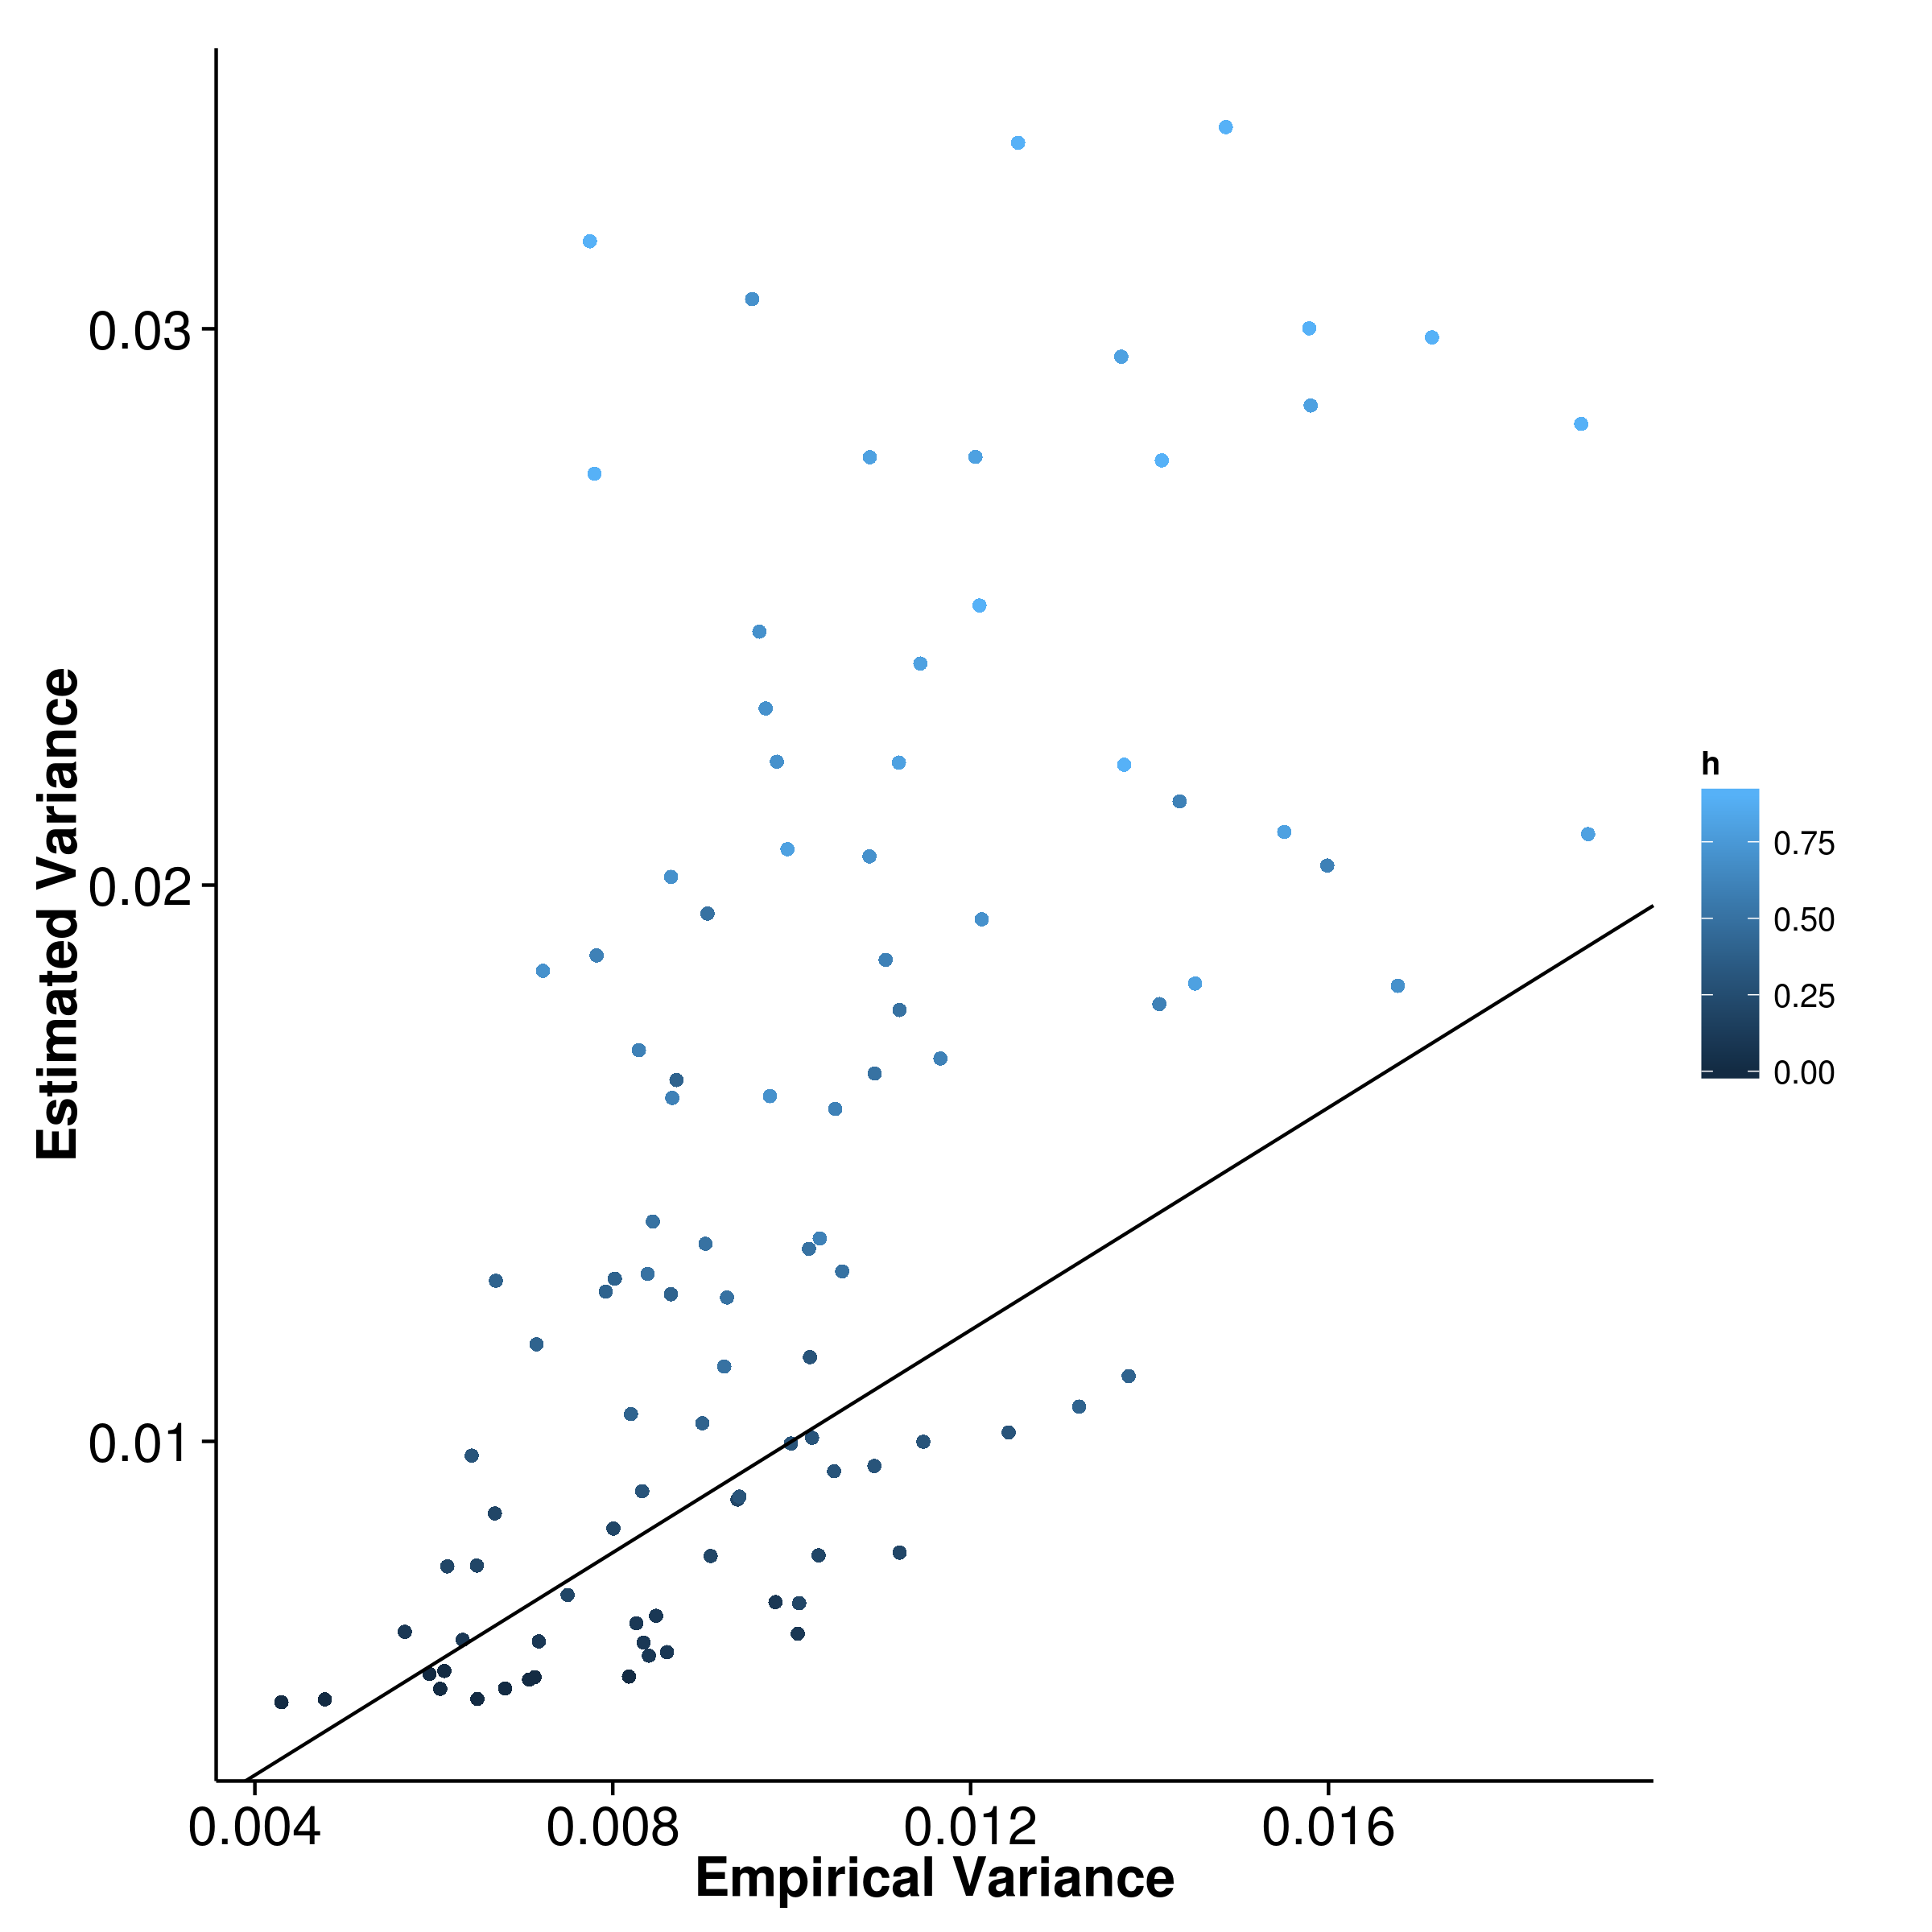
\includegraphics{figure/quantitative/same_effect/100c/ldsc_50k_100c_varH.png}}
				\label{fig:50k100cQtvarL}
			}
			\subfloat[LDSC with intercept estimation]{
				\scalebox{.4}{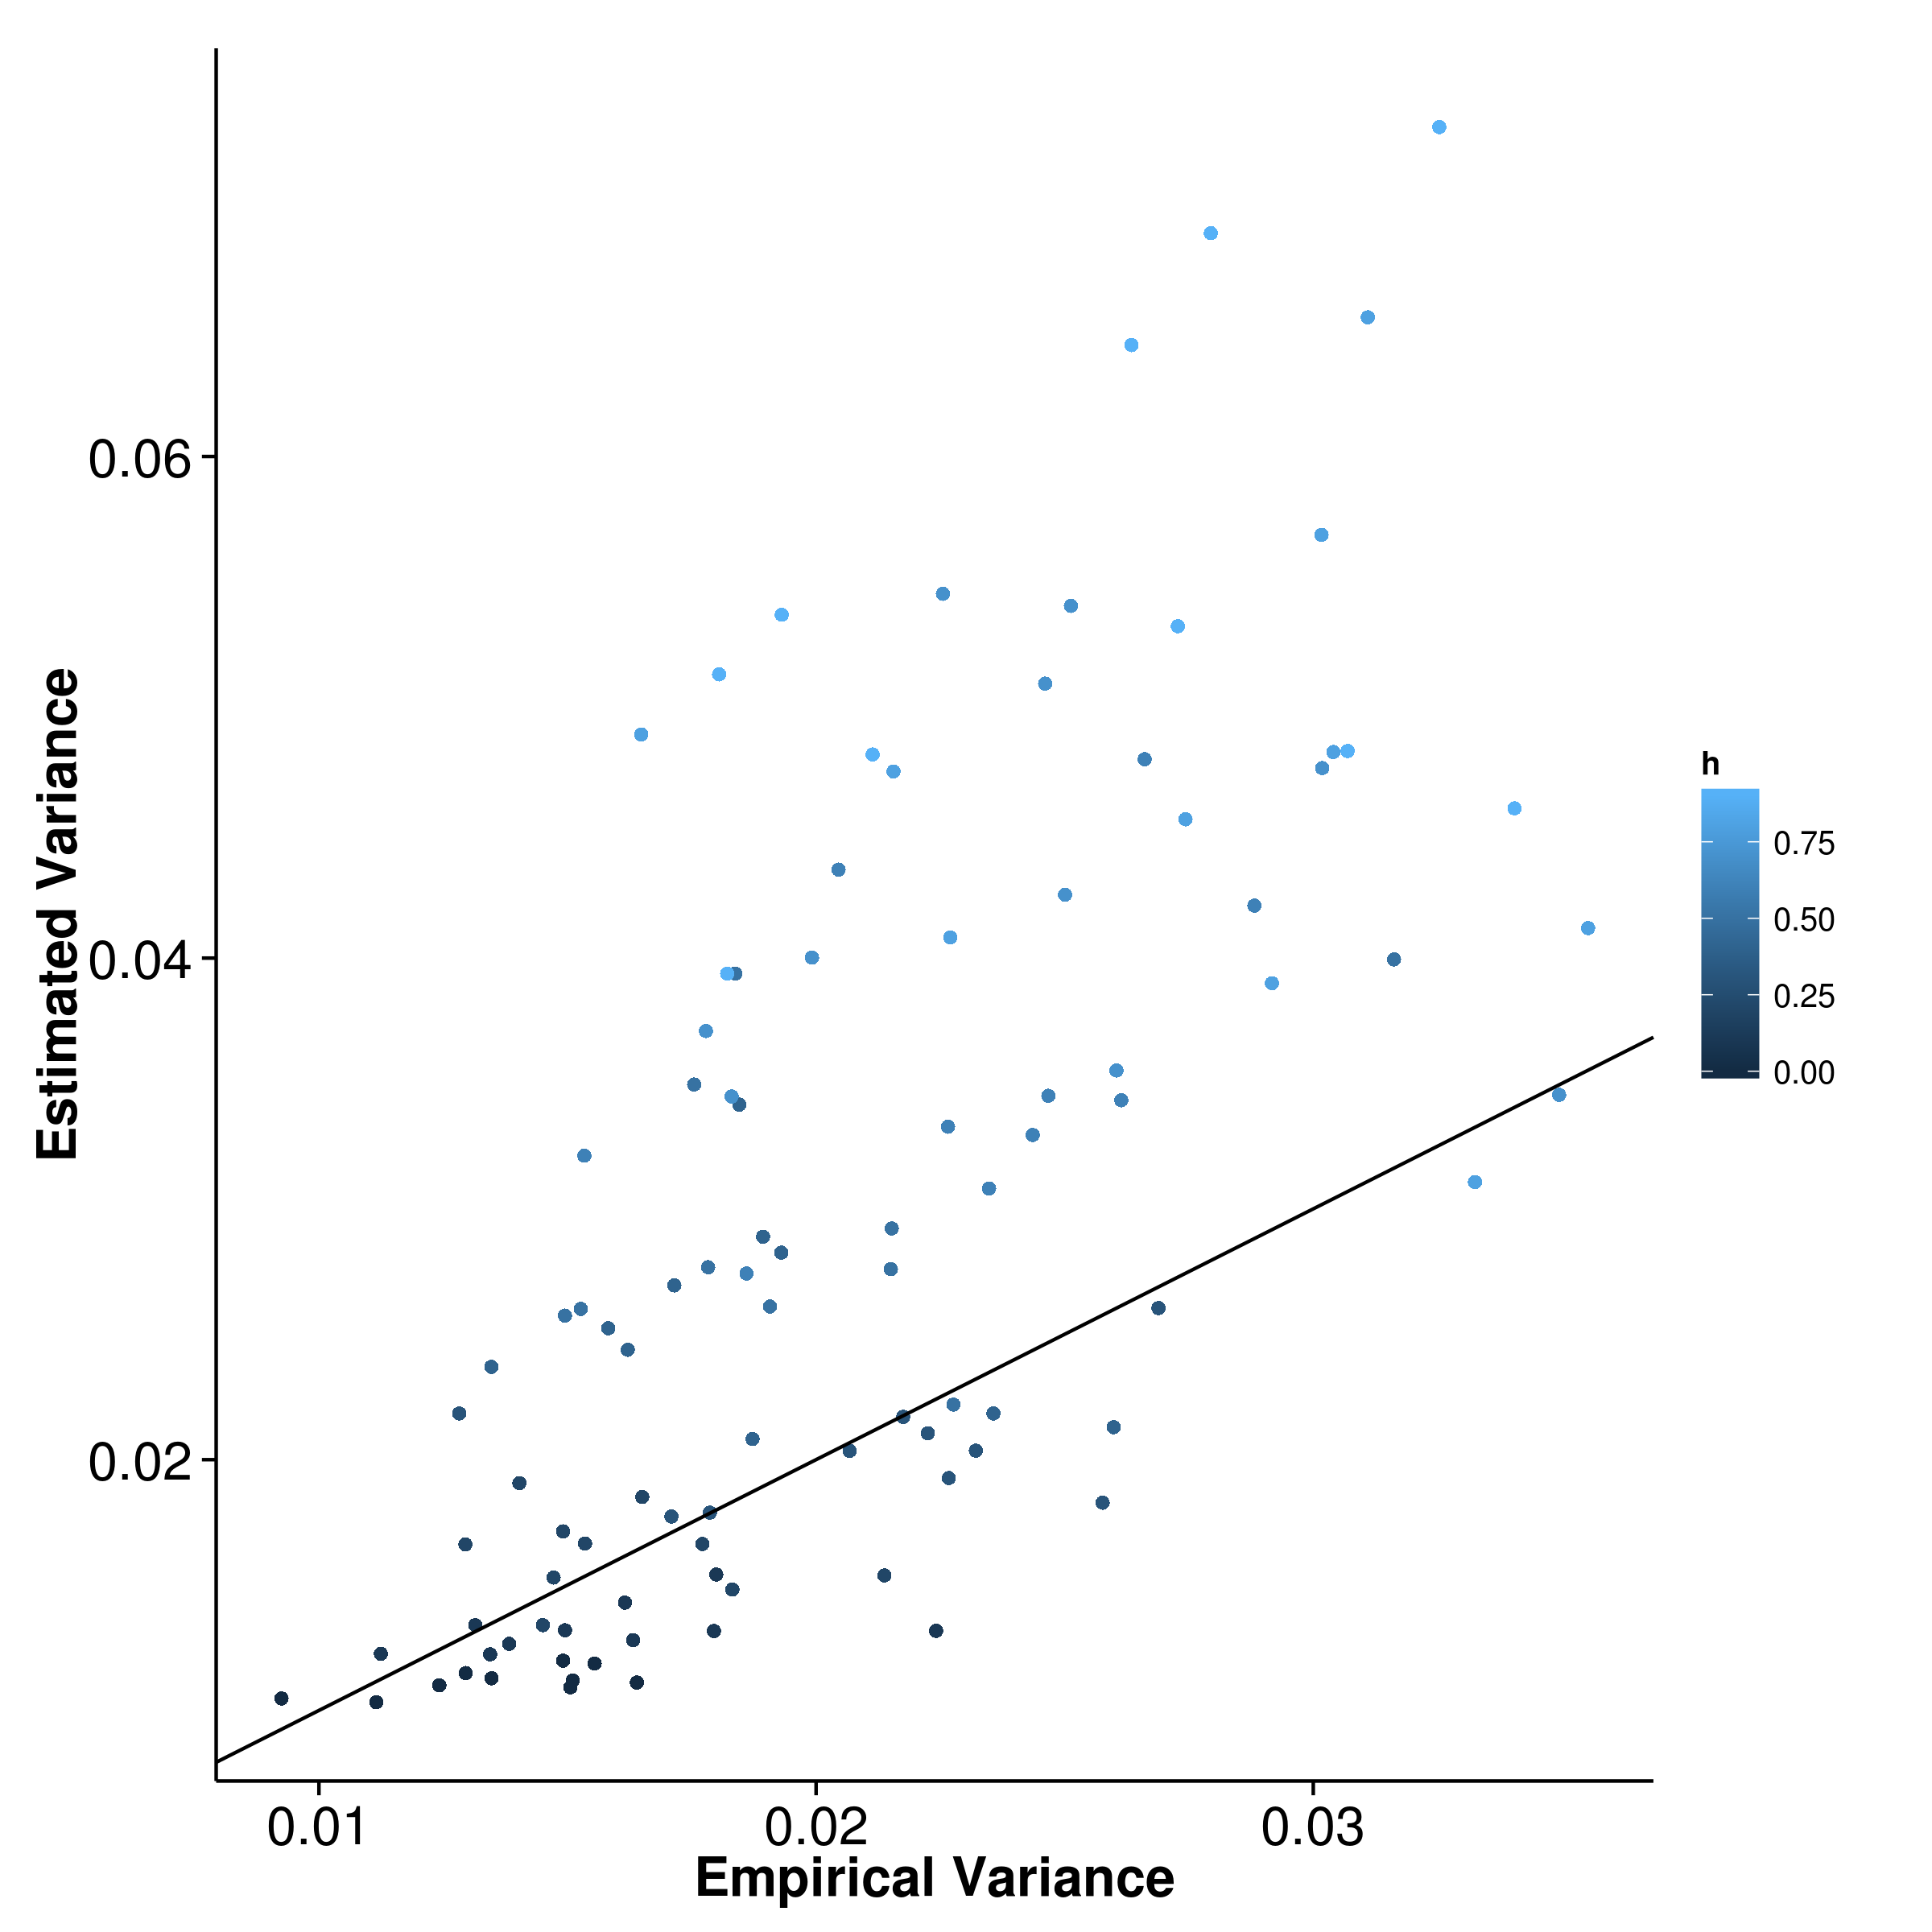
\includegraphics{figure/quantitative/same_effect/100c/ldscIn_50k_100c_varH.png}}
				\label{fig:50k100cQtvarI}
			}
			\label{fig:50k100cQtVar}
		\end{figure}
		
		
		\begin{figure}
			\centering
			\centering
			\subfloat[SHREK]{
				\scalebox{.4}{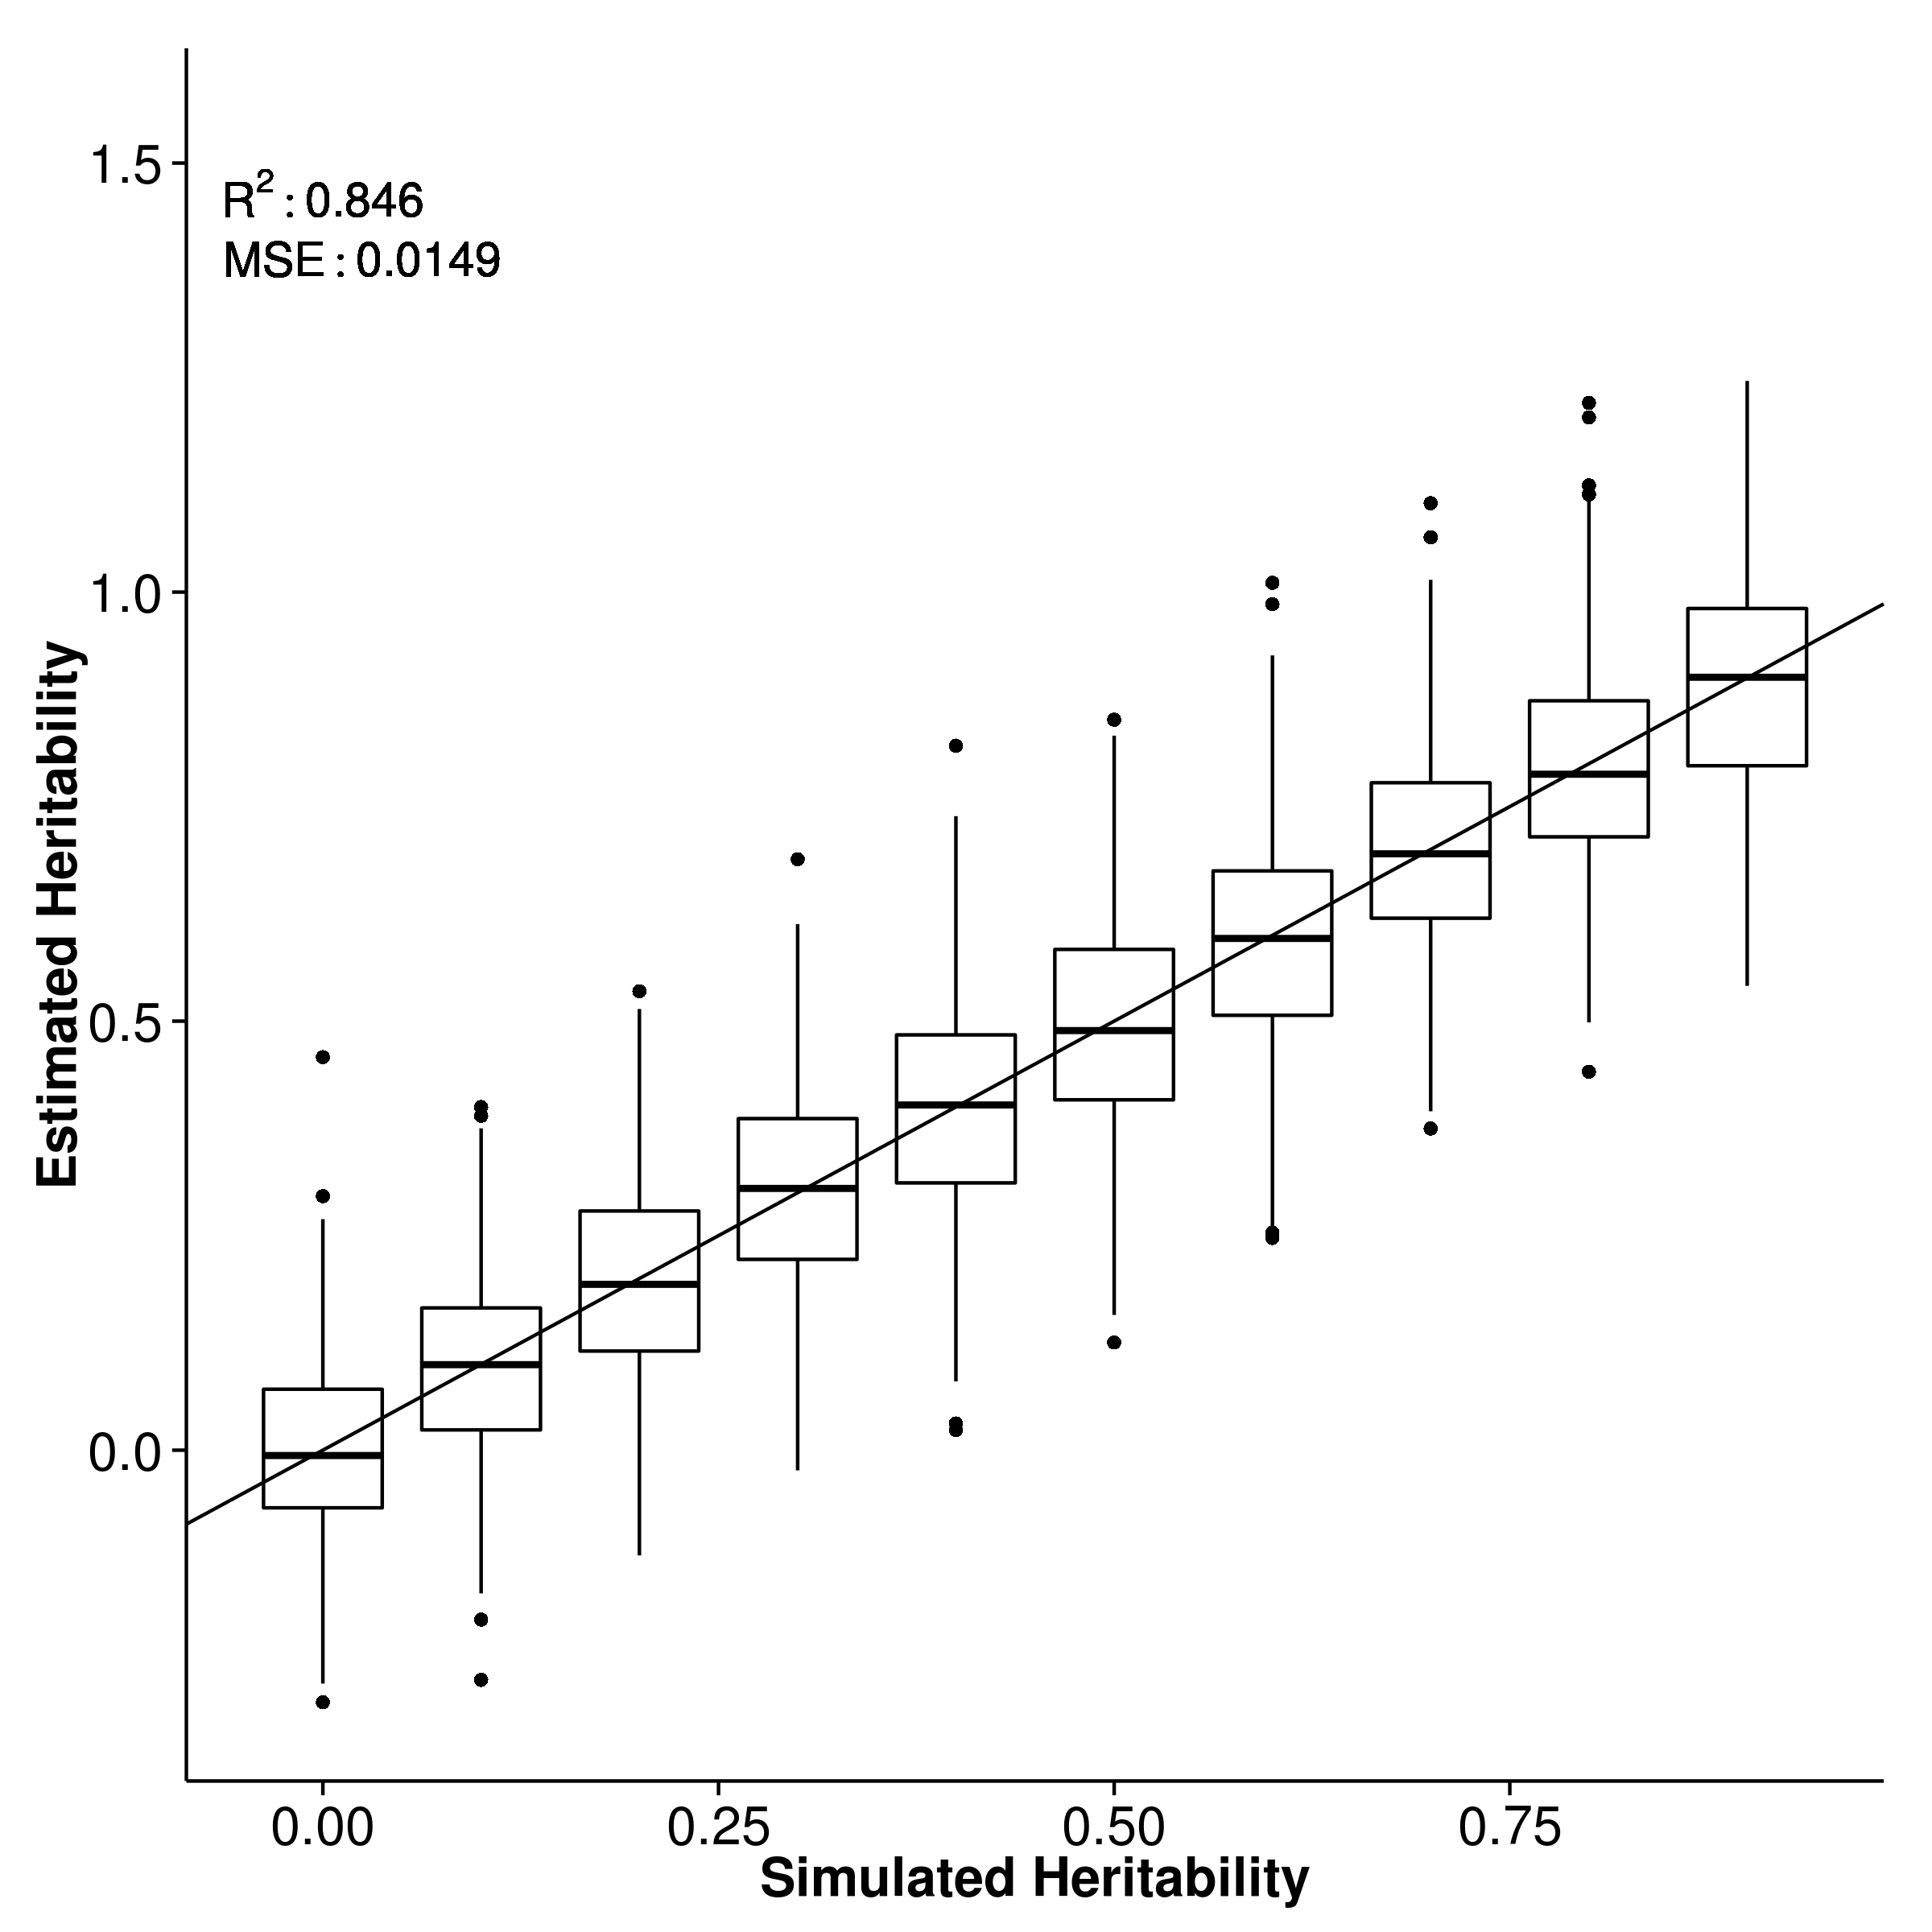
\includegraphics{figure/quantitative/same_effect/250c/shrek_50k_250c_meanH.png}}
				\label{fig:50k250cQtmeanS}
			}
			\subfloat[GCTA]{
				\scalebox{.4}{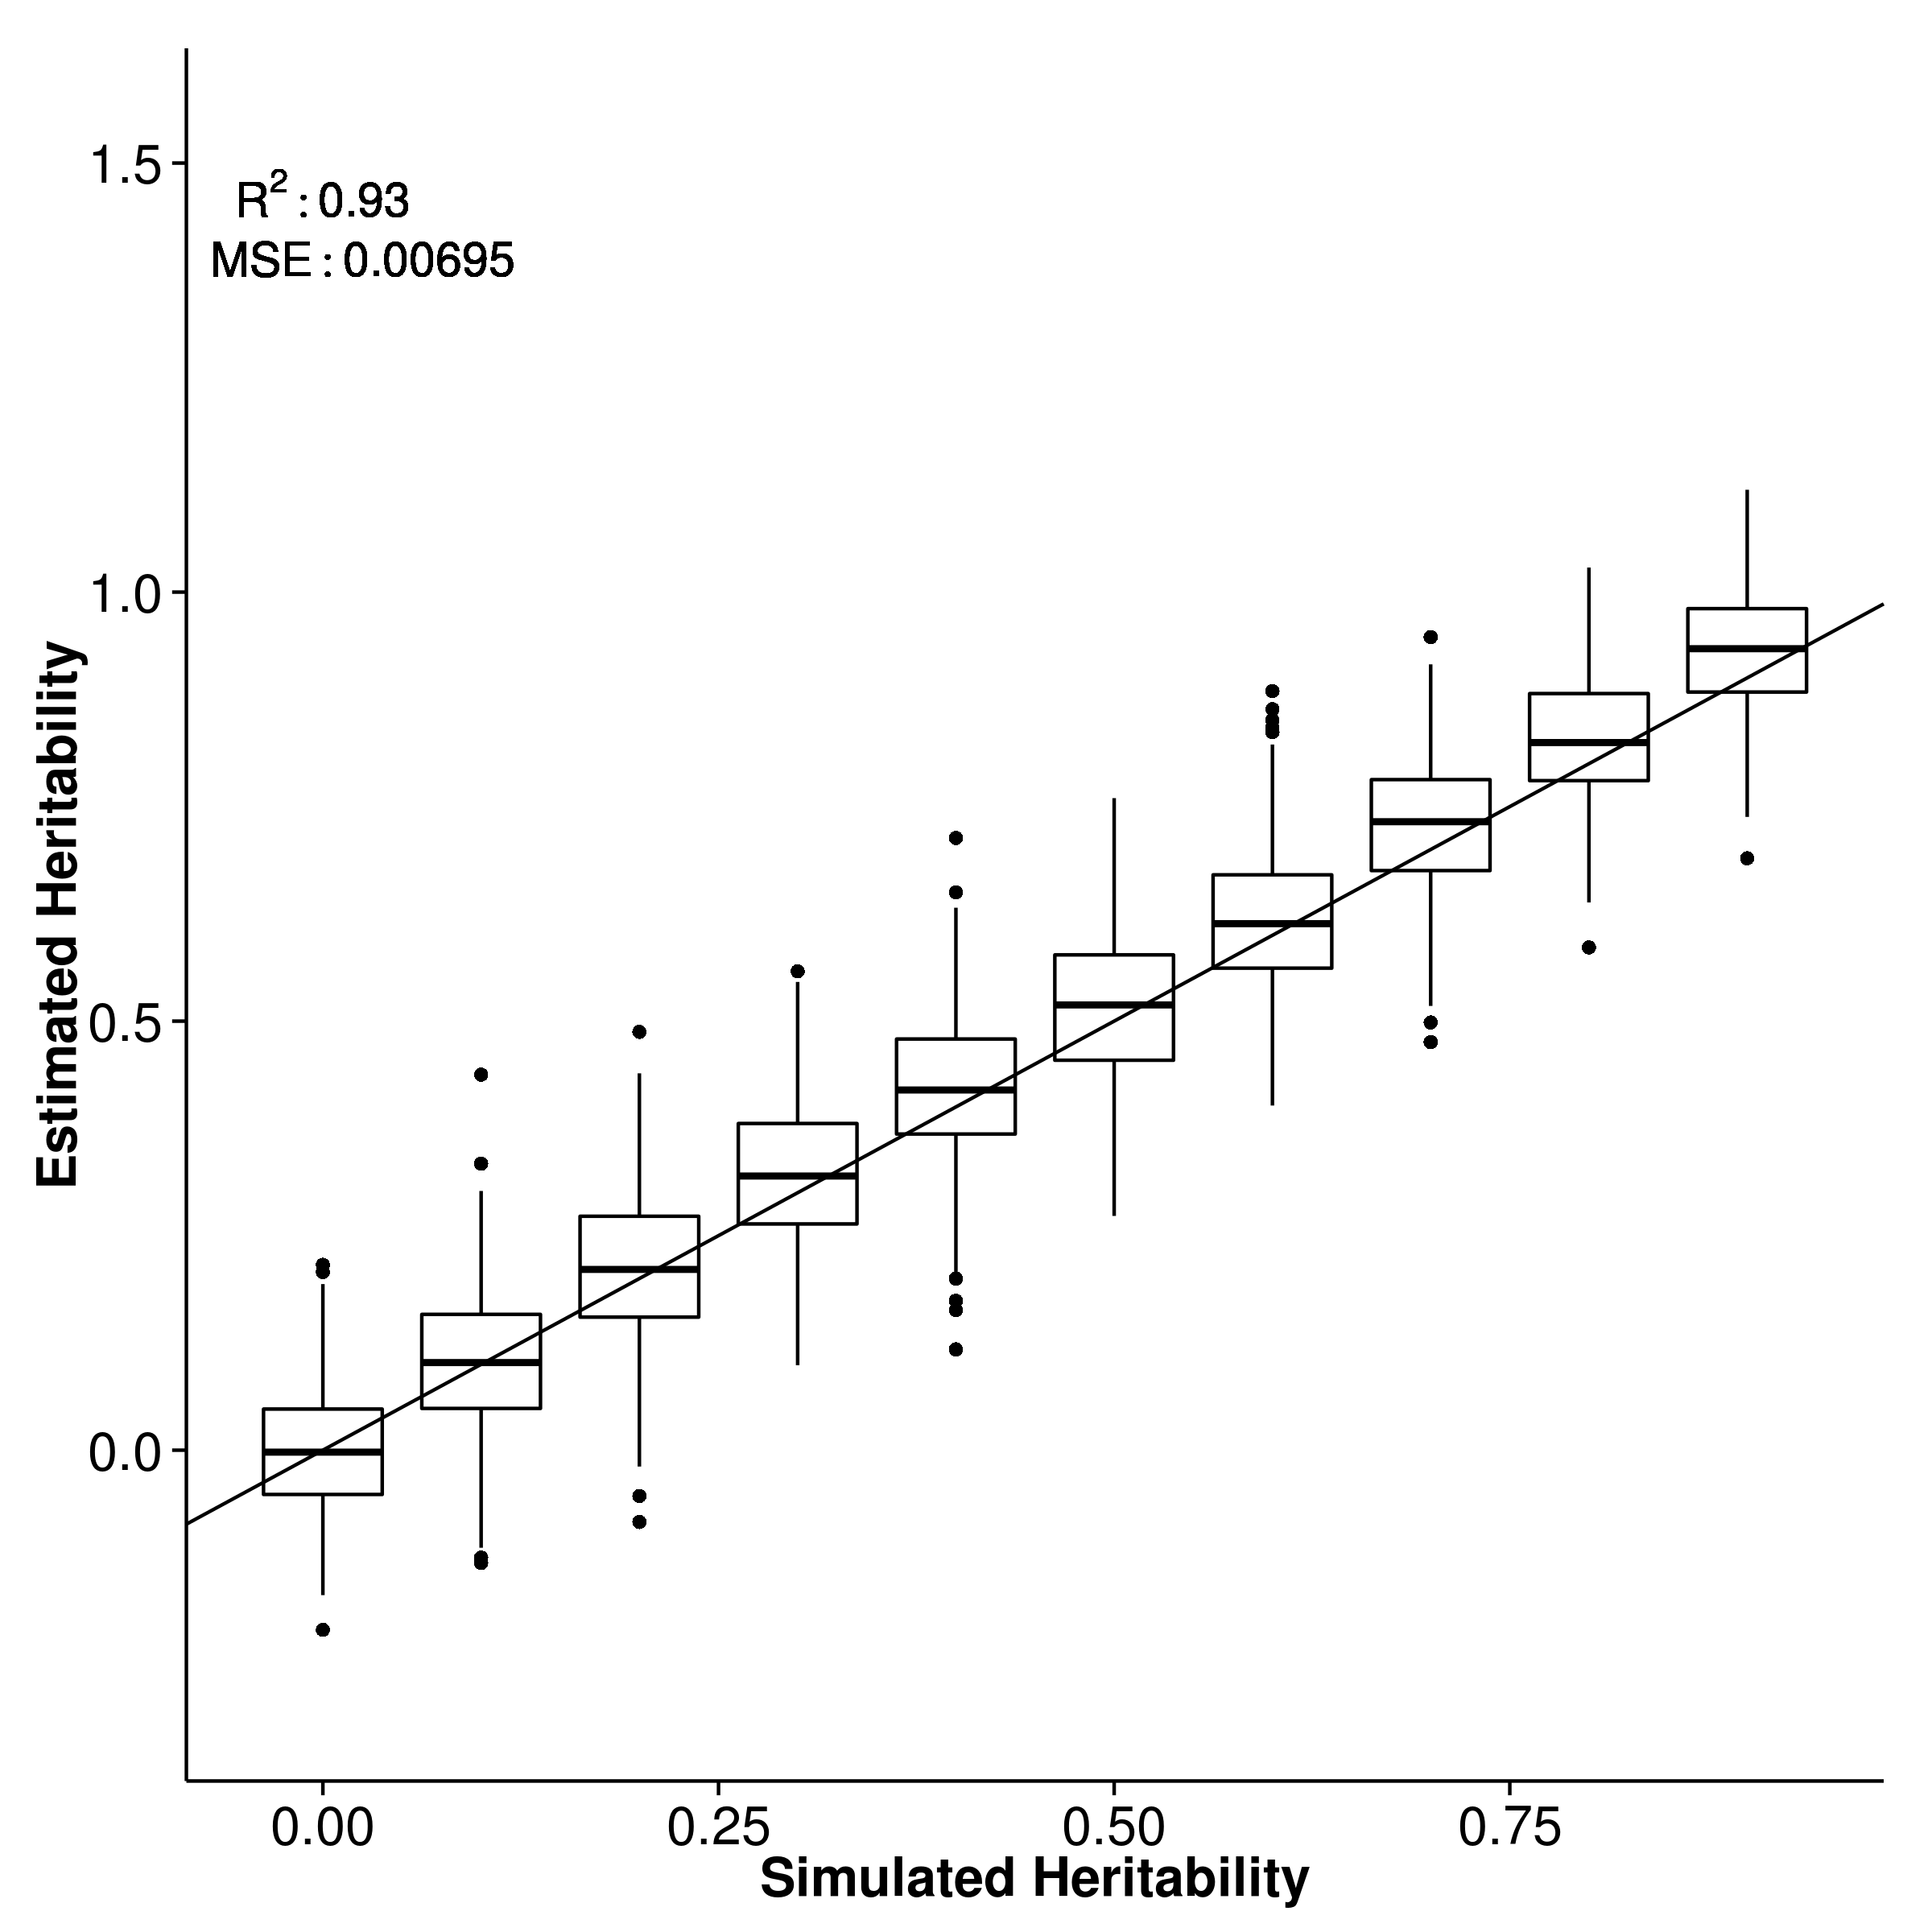
\includegraphics{figure/quantitative/same_effect/250c/gcta_50k_250c_meanH.png}}
				\label{fig:50k250cQtmeanG}
			}\\
			\subfloat[LDSC with fix intercept]{
				\scalebox{.4}{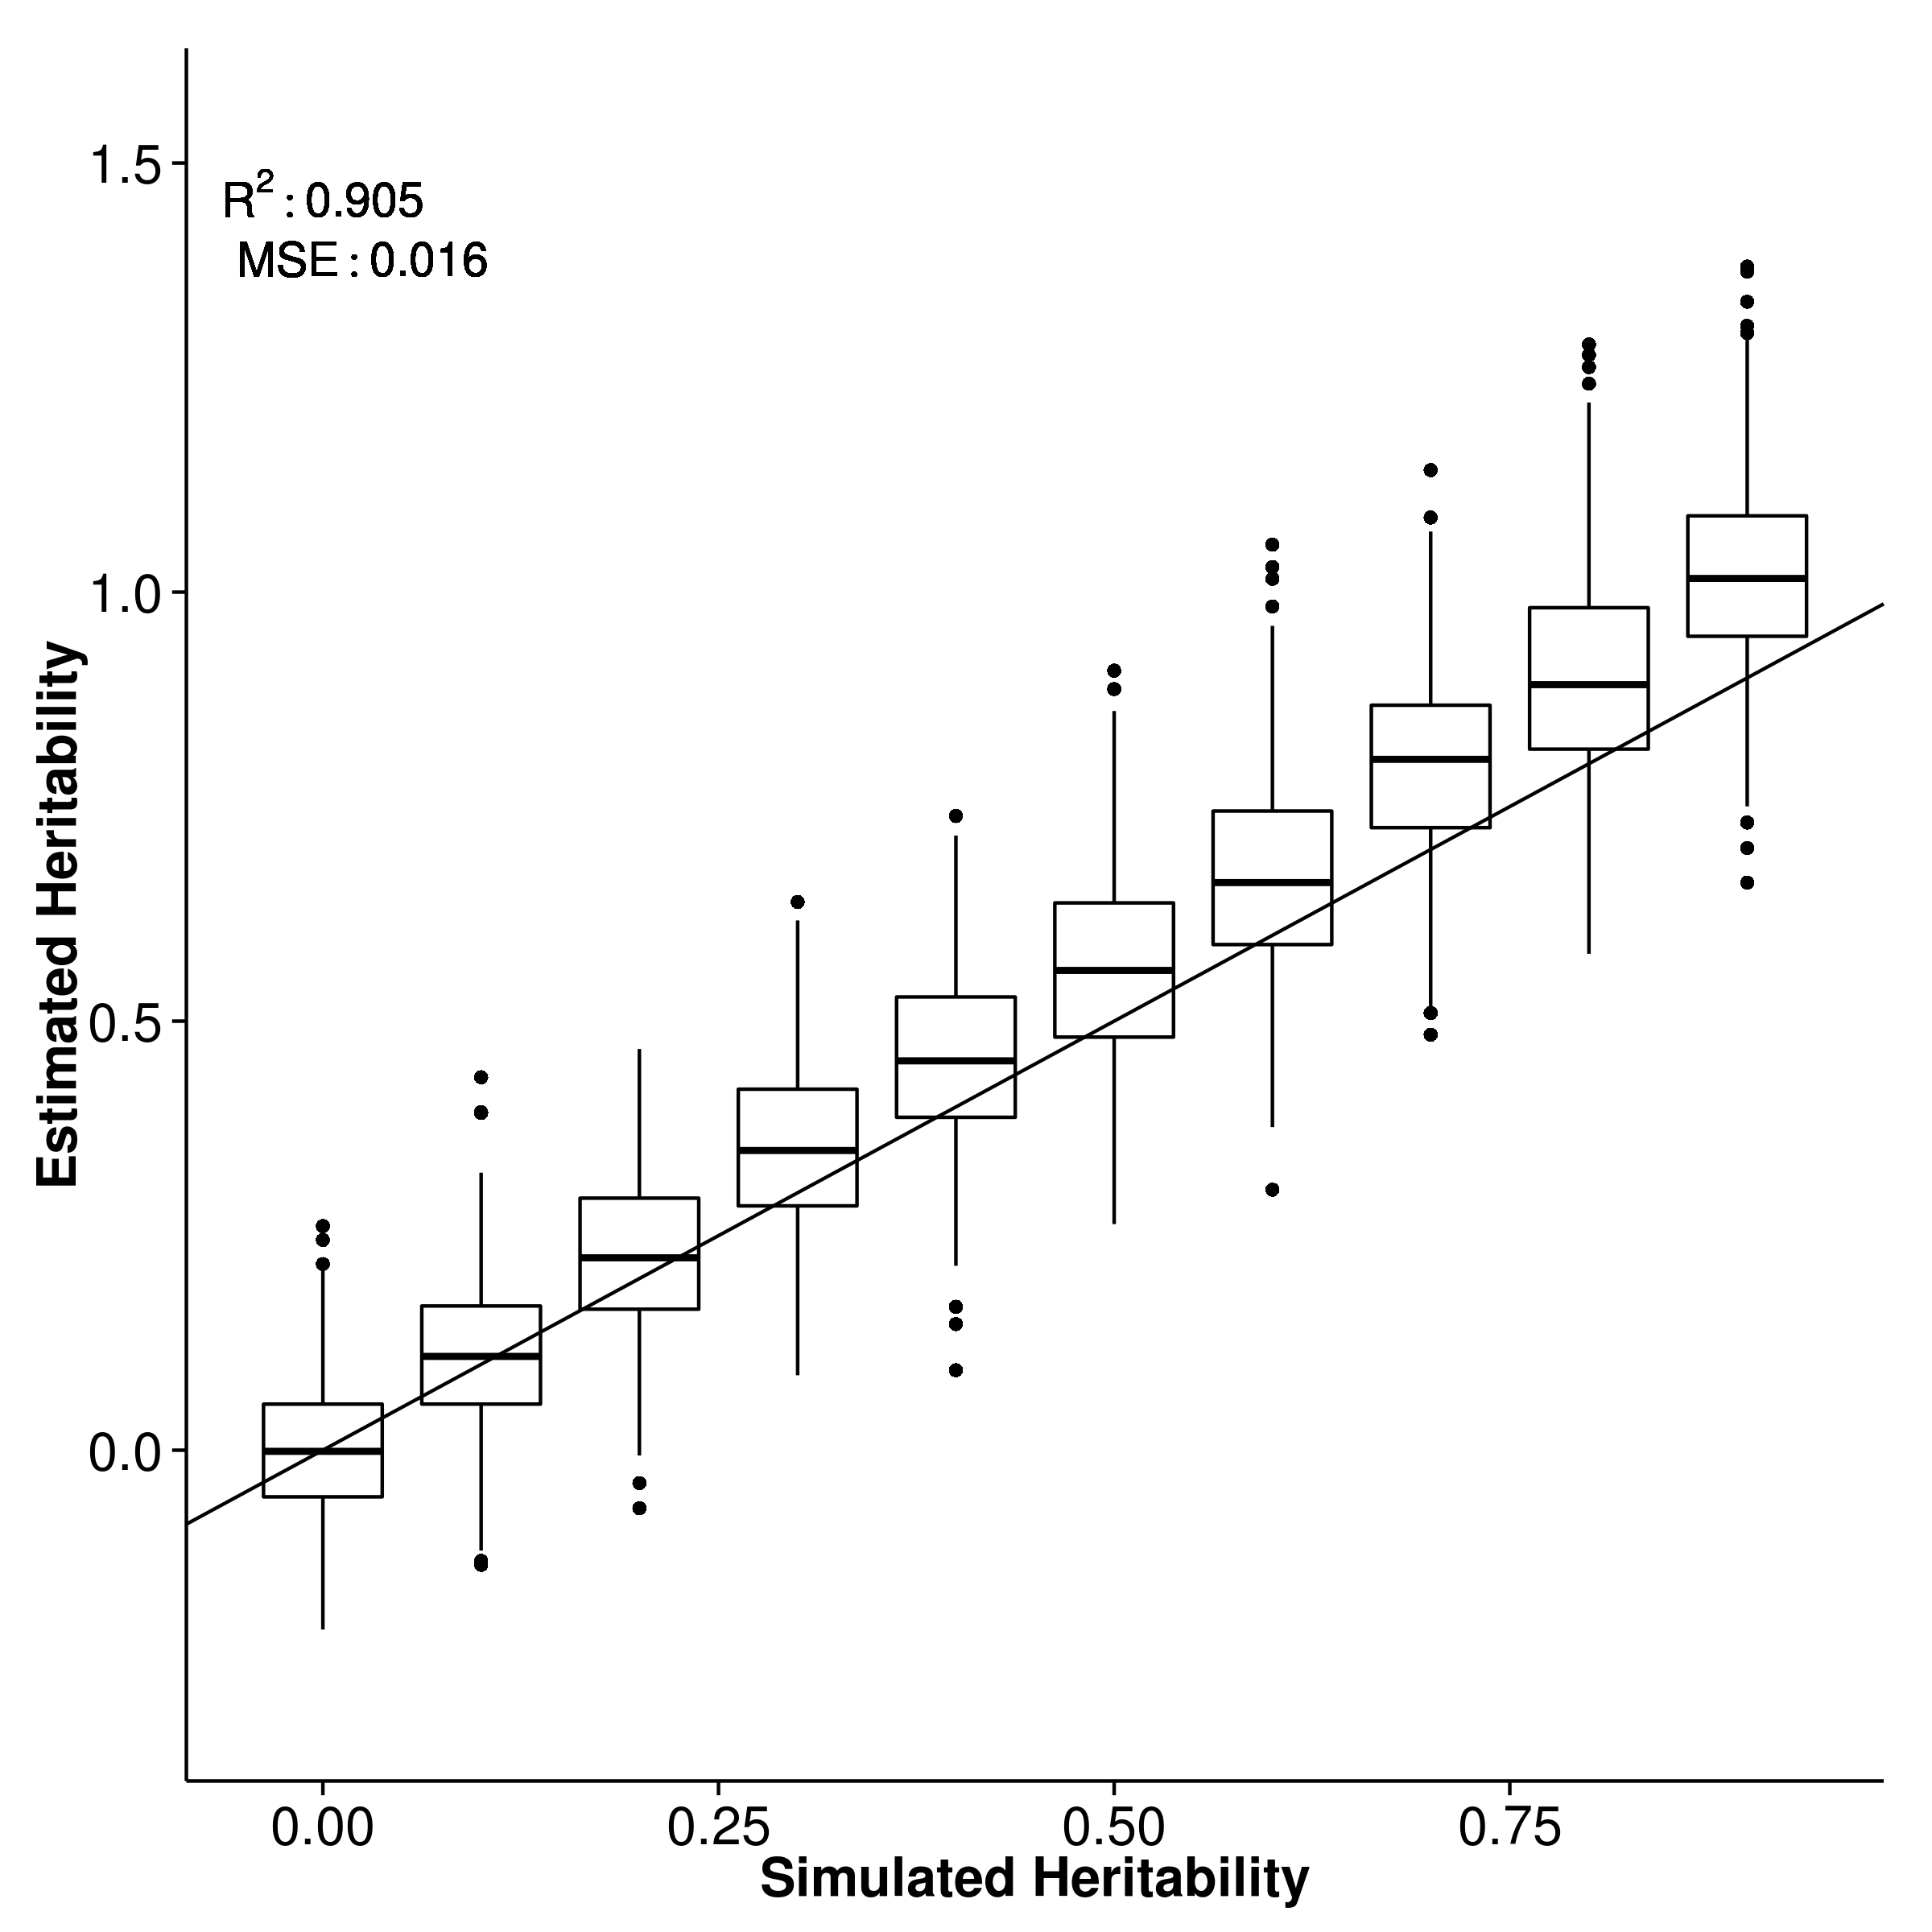
\includegraphics{figure/quantitative/same_effect/250c/ldsc_50k_250c_meanH.png}}
				\label{fig:50k250cQtmeanL}
			}
			\subfloat[LDSC with intercept estimation]{
				\scalebox{.4}{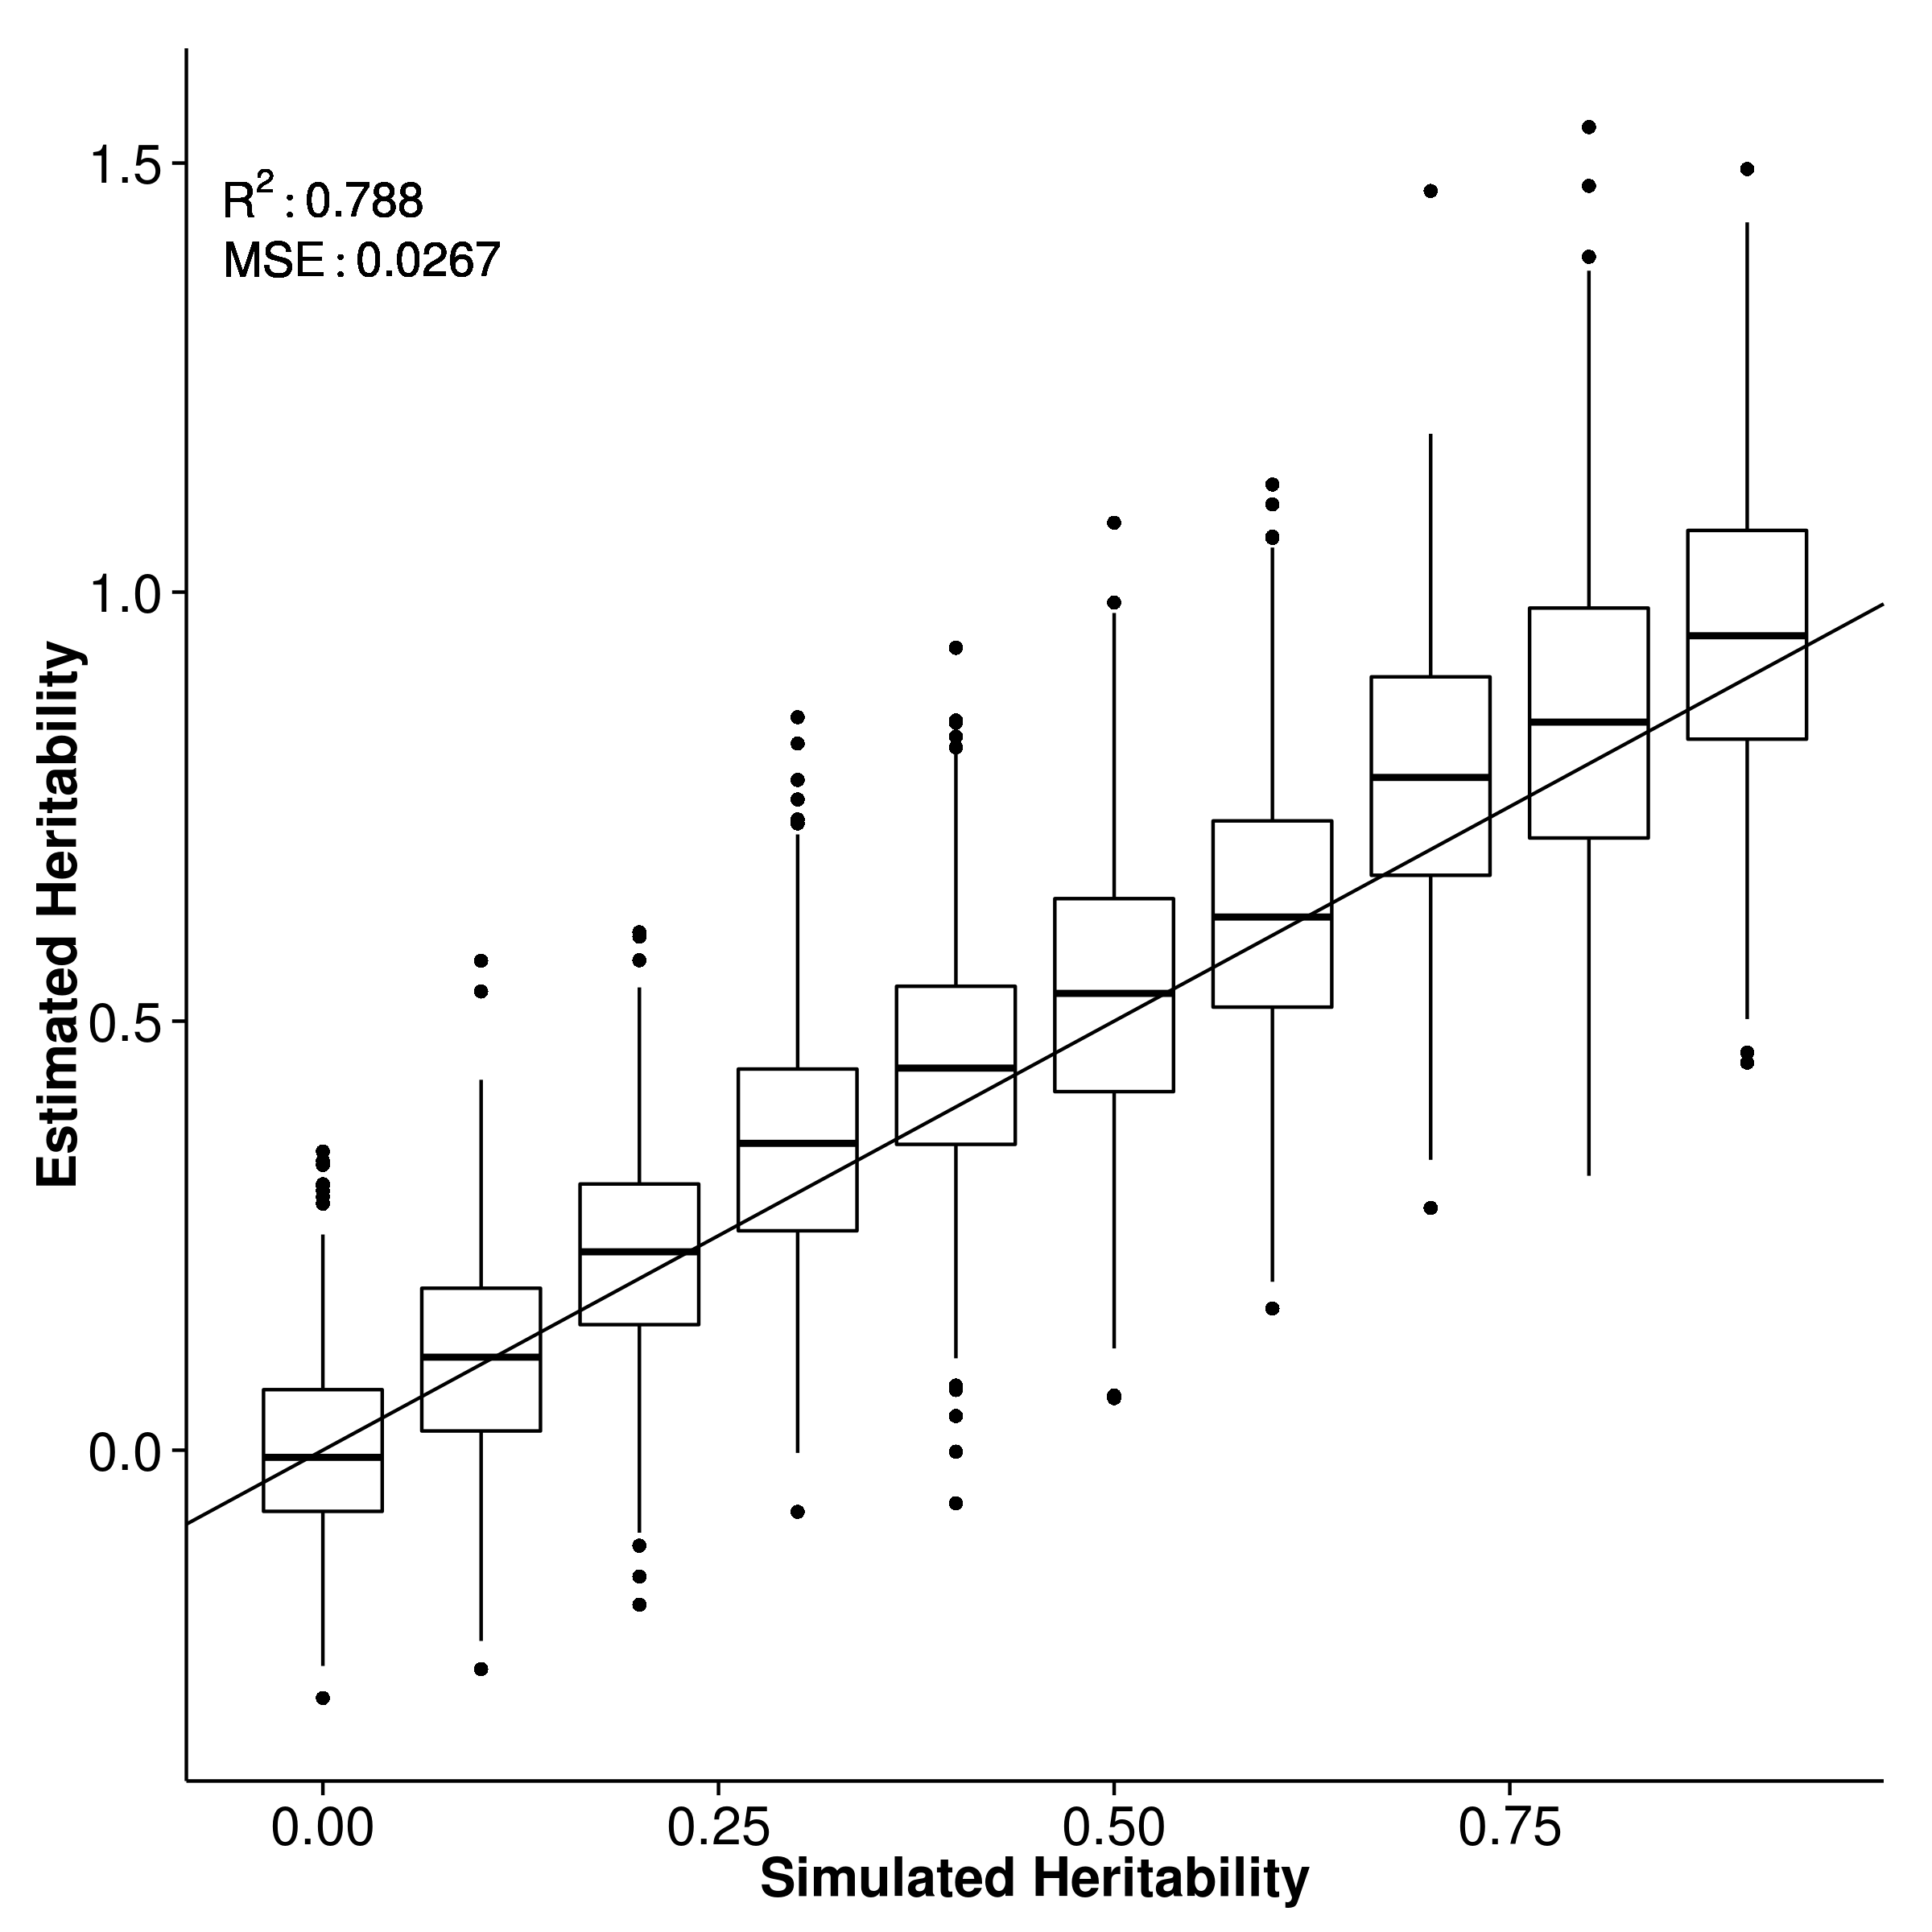
\includegraphics{figure/quantitative/same_effect/250c/ldscIn_50k_250c_meanH.png}}
				\label{fig:50k250cQtmeanI}
			}
			\caption[Simulation of Quantitative Traits with 50k \glsentryshortpl{SNP} and 250 causal variants of same effect size]
			{Simulation of Quantitative Traits with 50k \glsentryshortpl{SNP} and 250 causal variants with same effect size.} 
			\label{fig:50k250cQtMean}
		\end{figure}
		\begin{figure}
			\centering
			\centering
			\subfloat[SHREK]{
				\scalebox{.4}{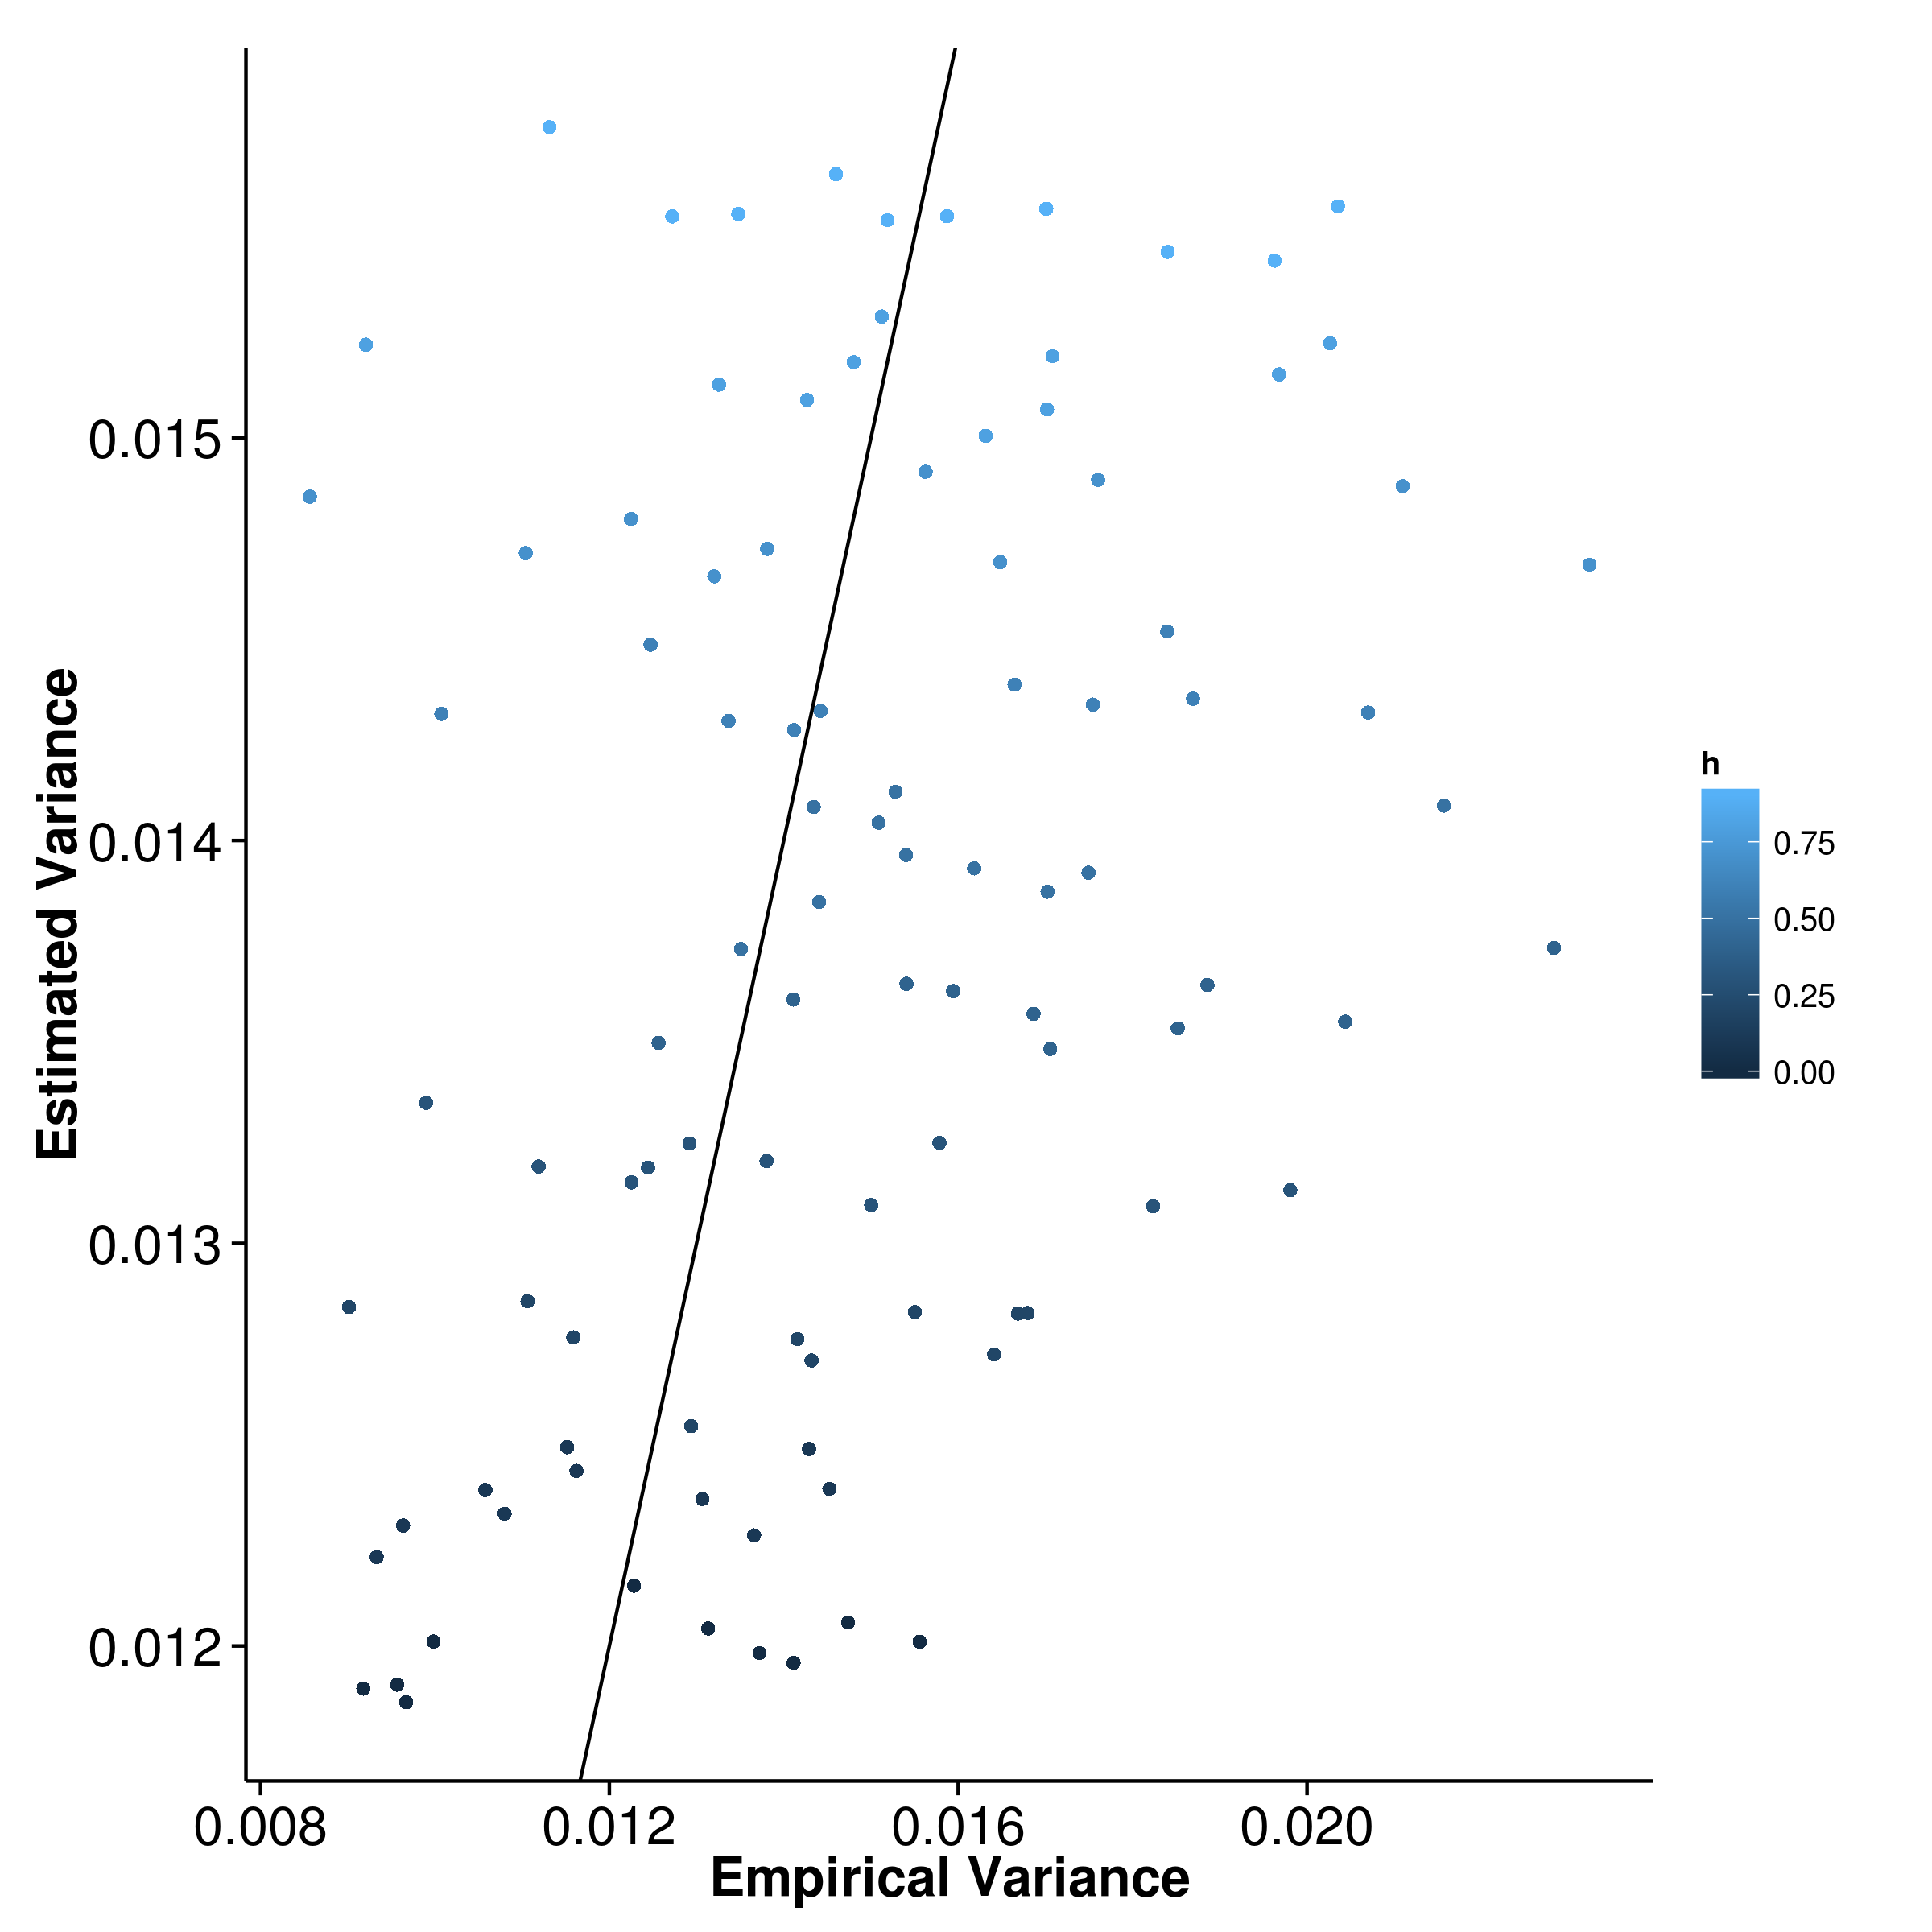
\includegraphics{figure/quantitative/same_effect/250c/shrek_50k_250c_varH.png}}
				\label{fig:50k250cQtvarS}
			}
			\subfloat[GCTA]{
				\scalebox{.4}{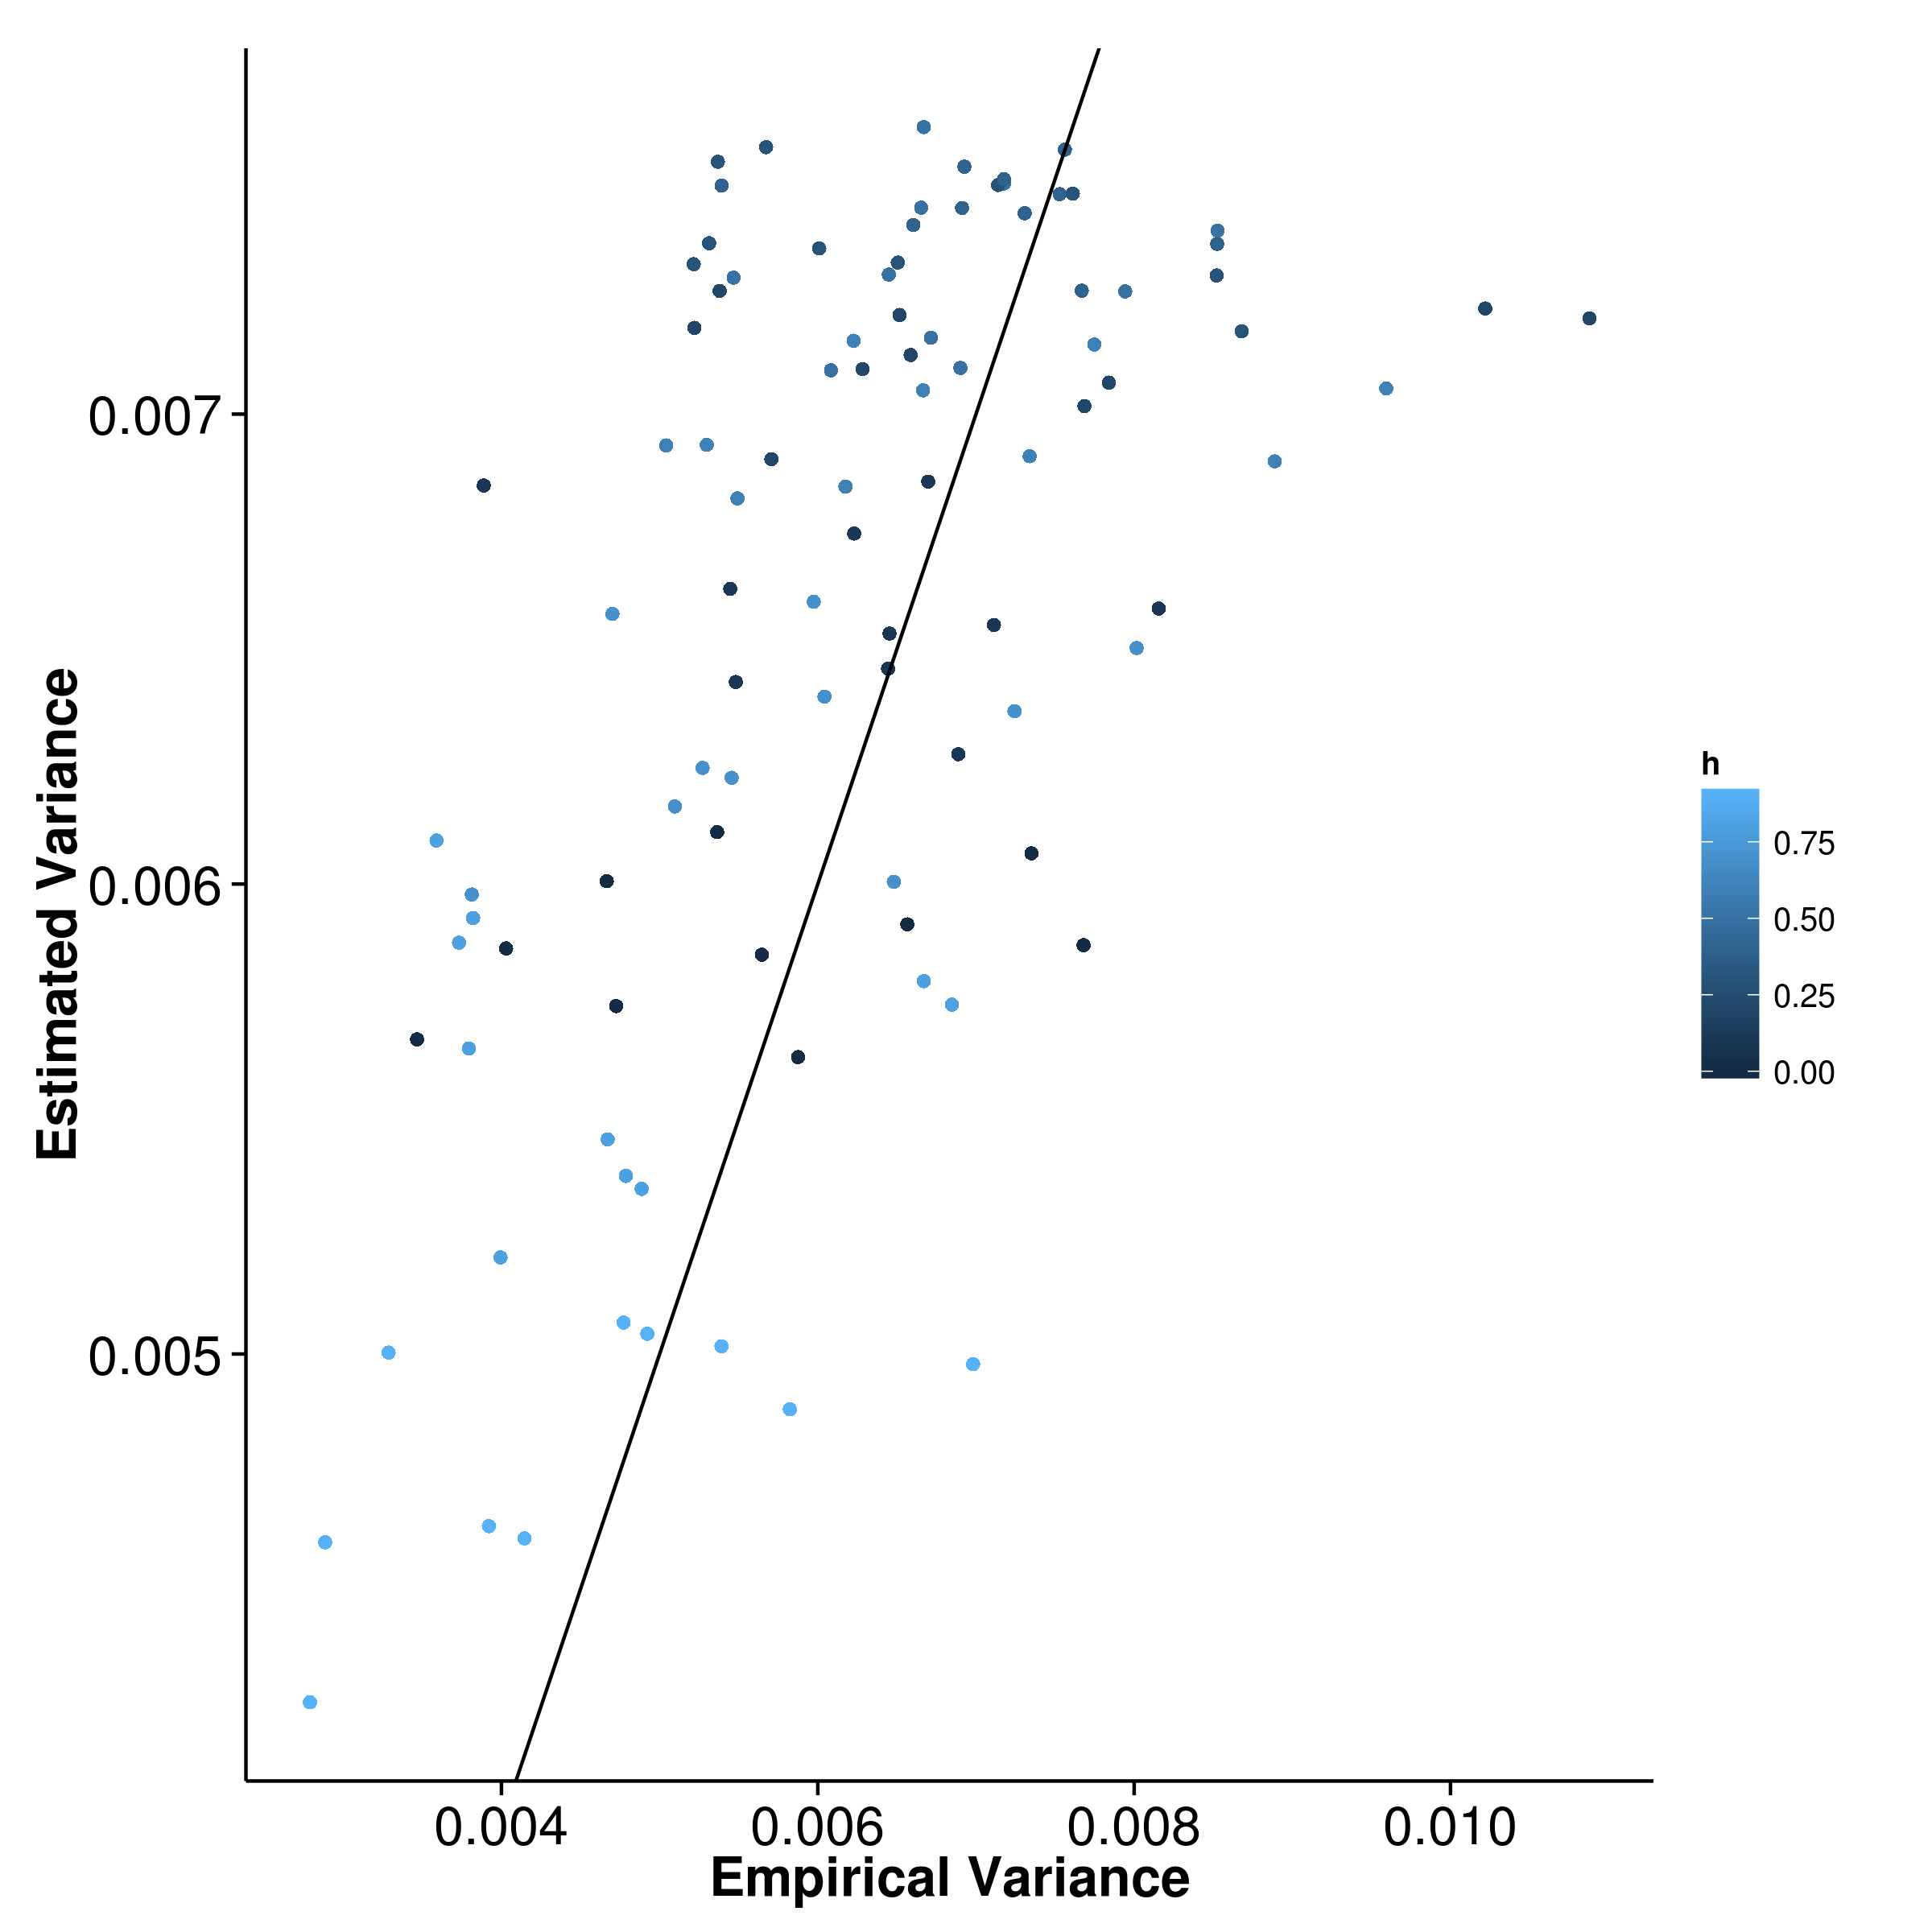
\includegraphics{figure/quantitative/same_effect/250c/gcta_50k_250c_varH.png}}
				\label{fig:50k250cQtvarG}
			}\\
			\subfloat[LDSC with fix intercept]{
				\scalebox{.4}{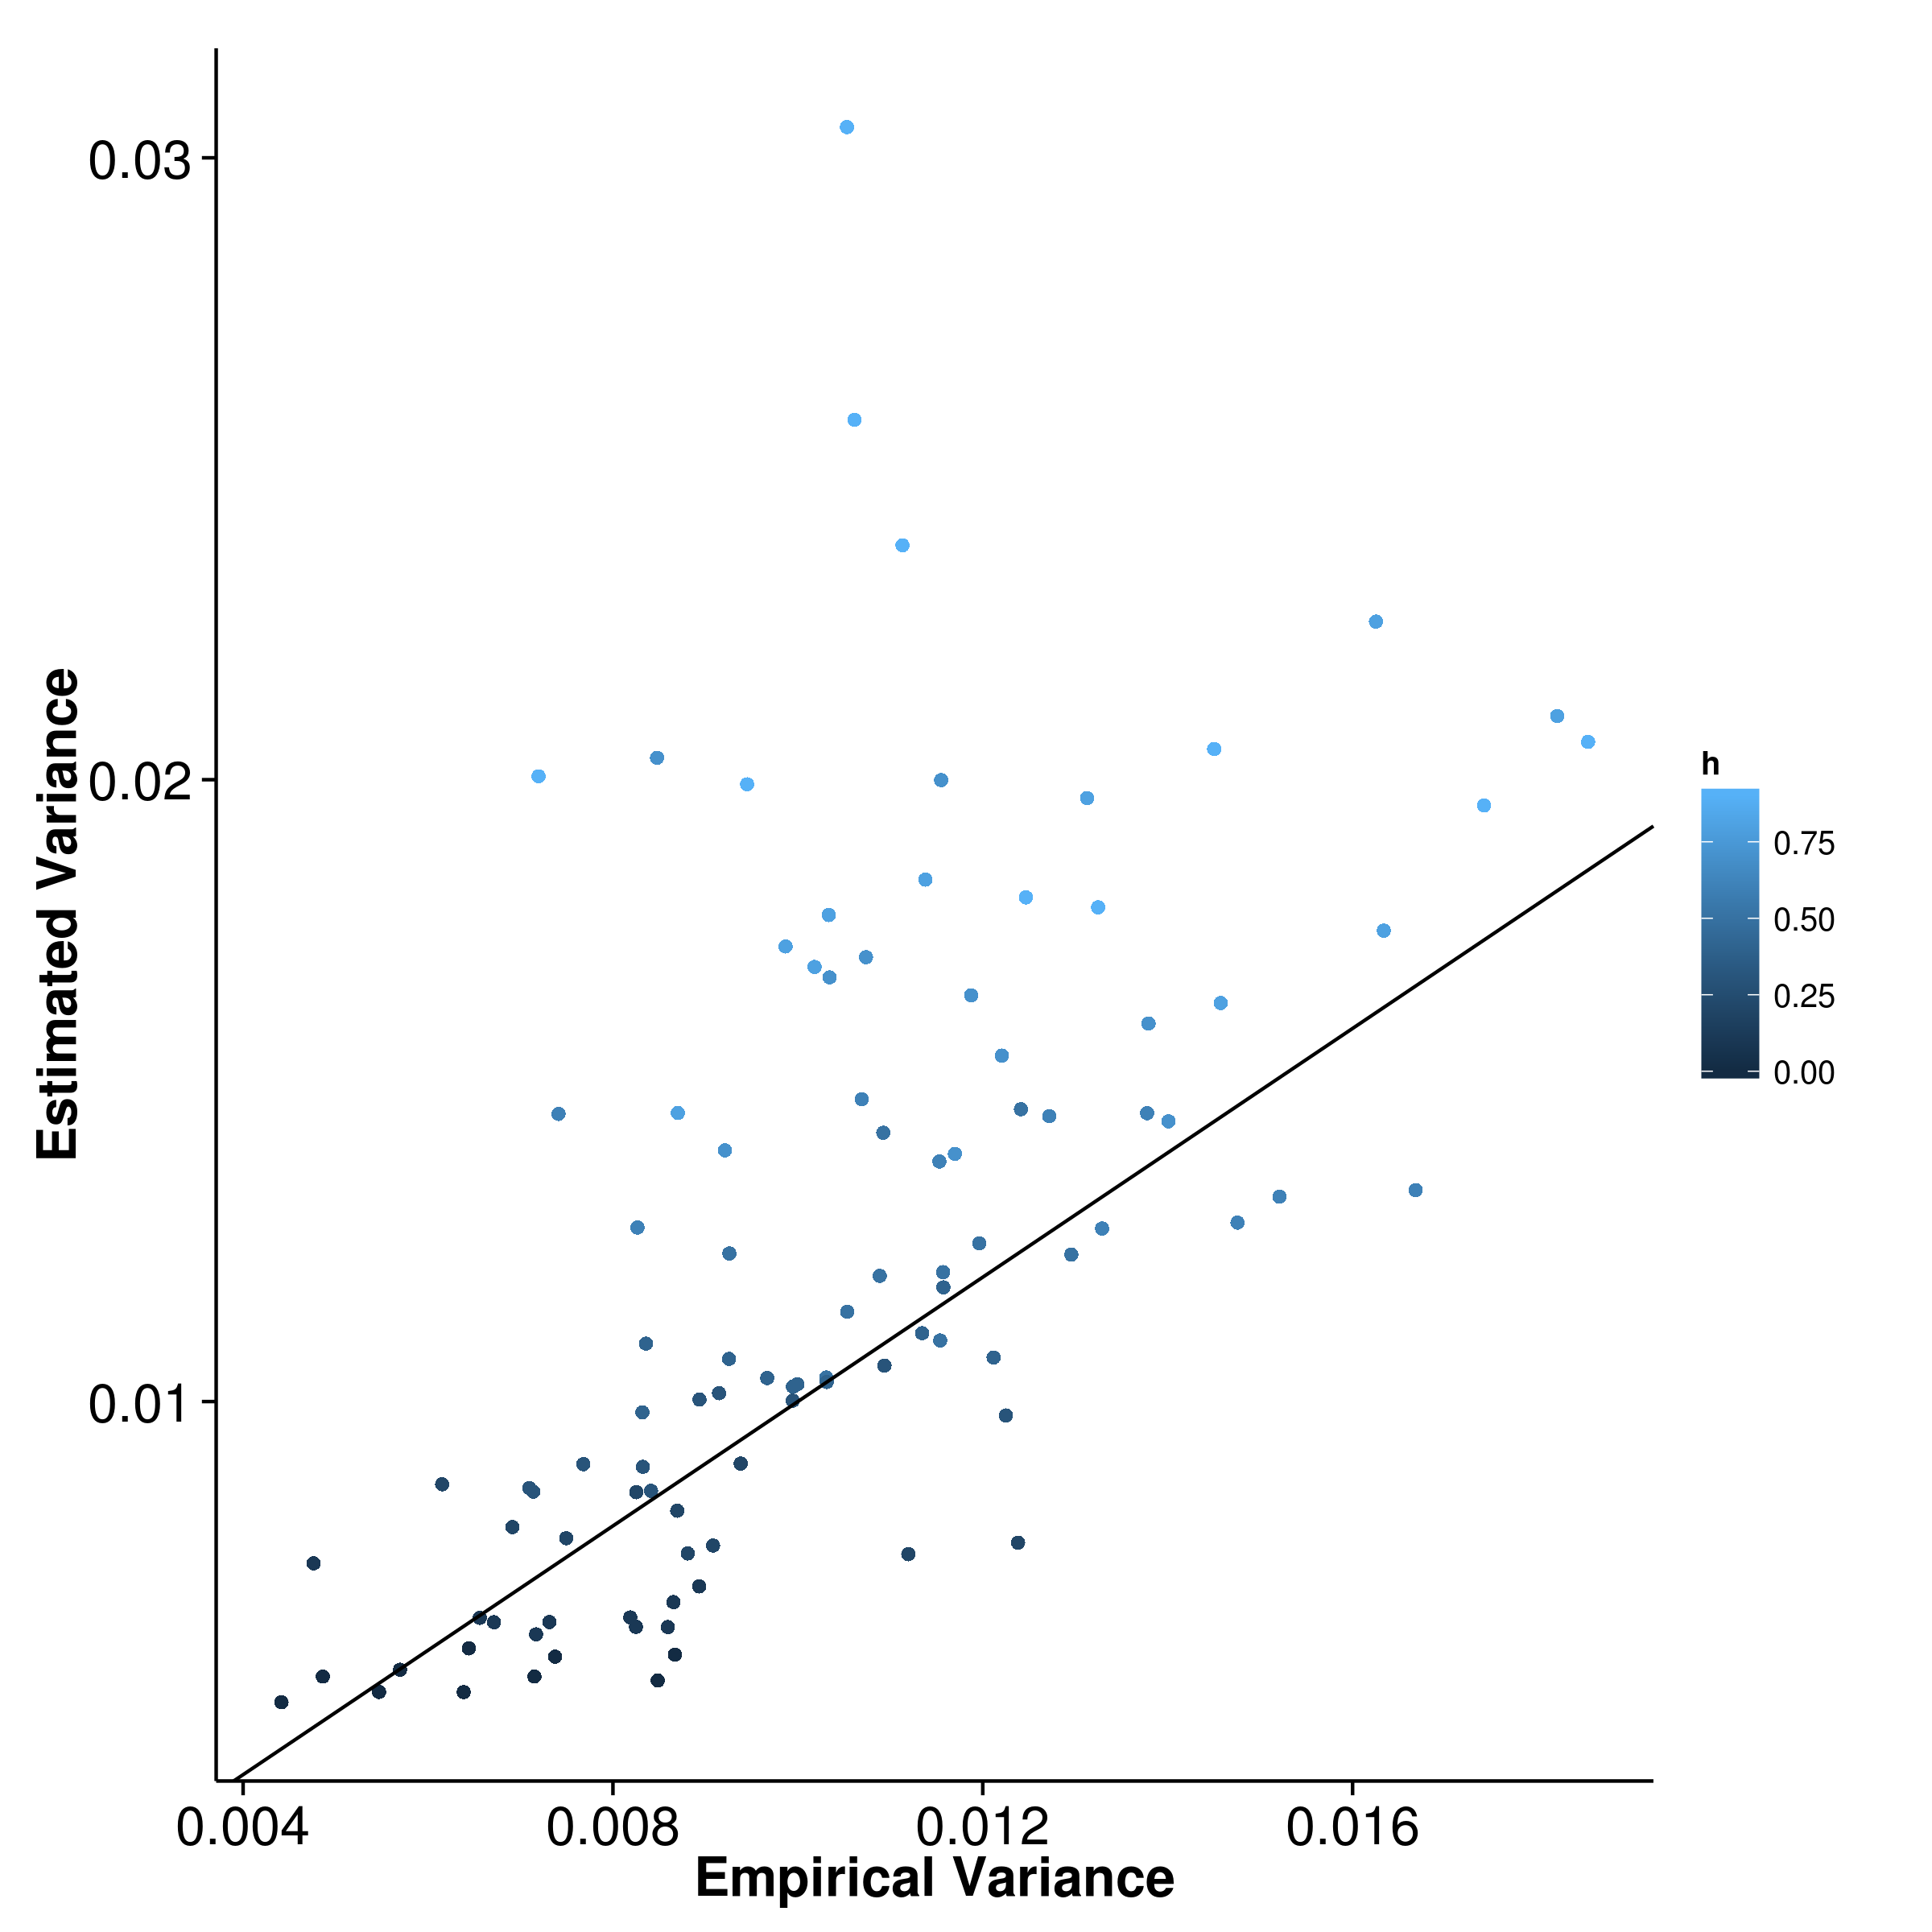
\includegraphics{figure/quantitative/same_effect/250c/ldsc_50k_250c_varH.png}}
				\label{fig:50k250cQtvarL}
			}
			\subfloat[LDSC with intercept estimation]{
				\scalebox{.4}{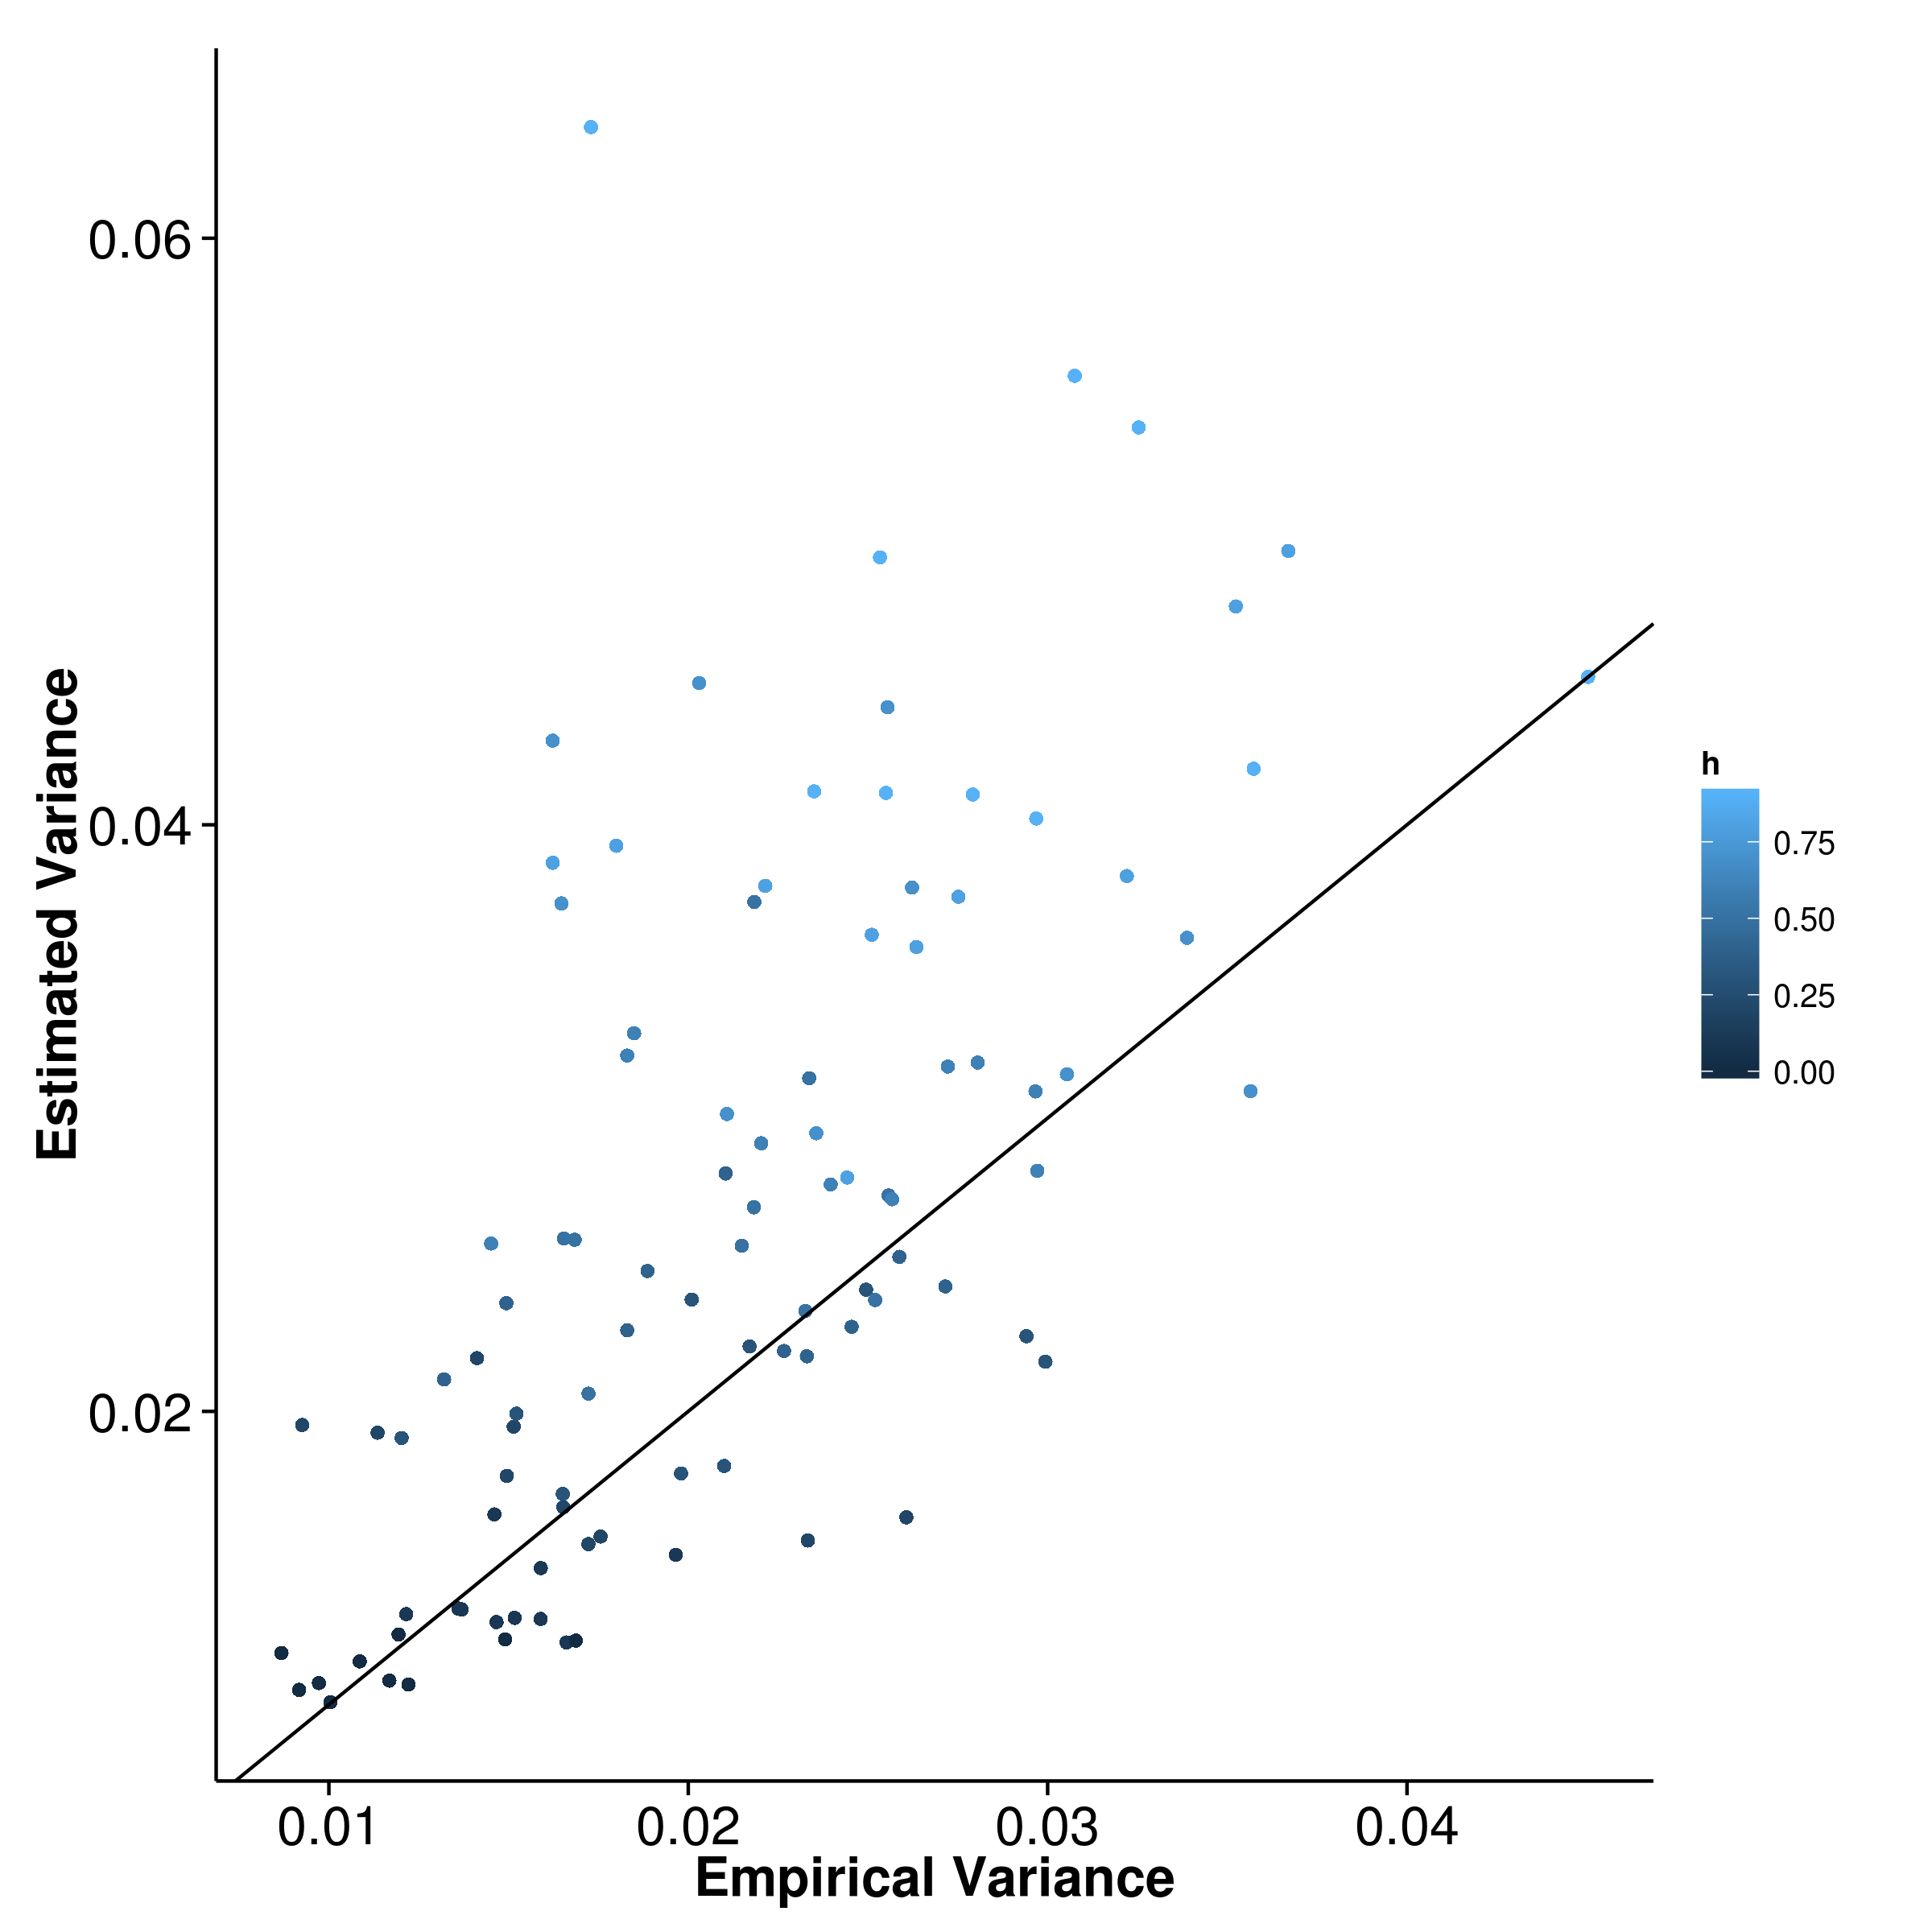
\includegraphics{figure/quantitative/same_effect/250c/ldscIn_50k_250c_varH.png}}
				\label{fig:50k250cQtvarI}
			}
			\label{fig:50k250cQtVar}
		\end{figure}
		
		
		
		\begin{figure}
			\centering
			\centering
			\subfloat[SHREK]{
				\scalebox{.4}{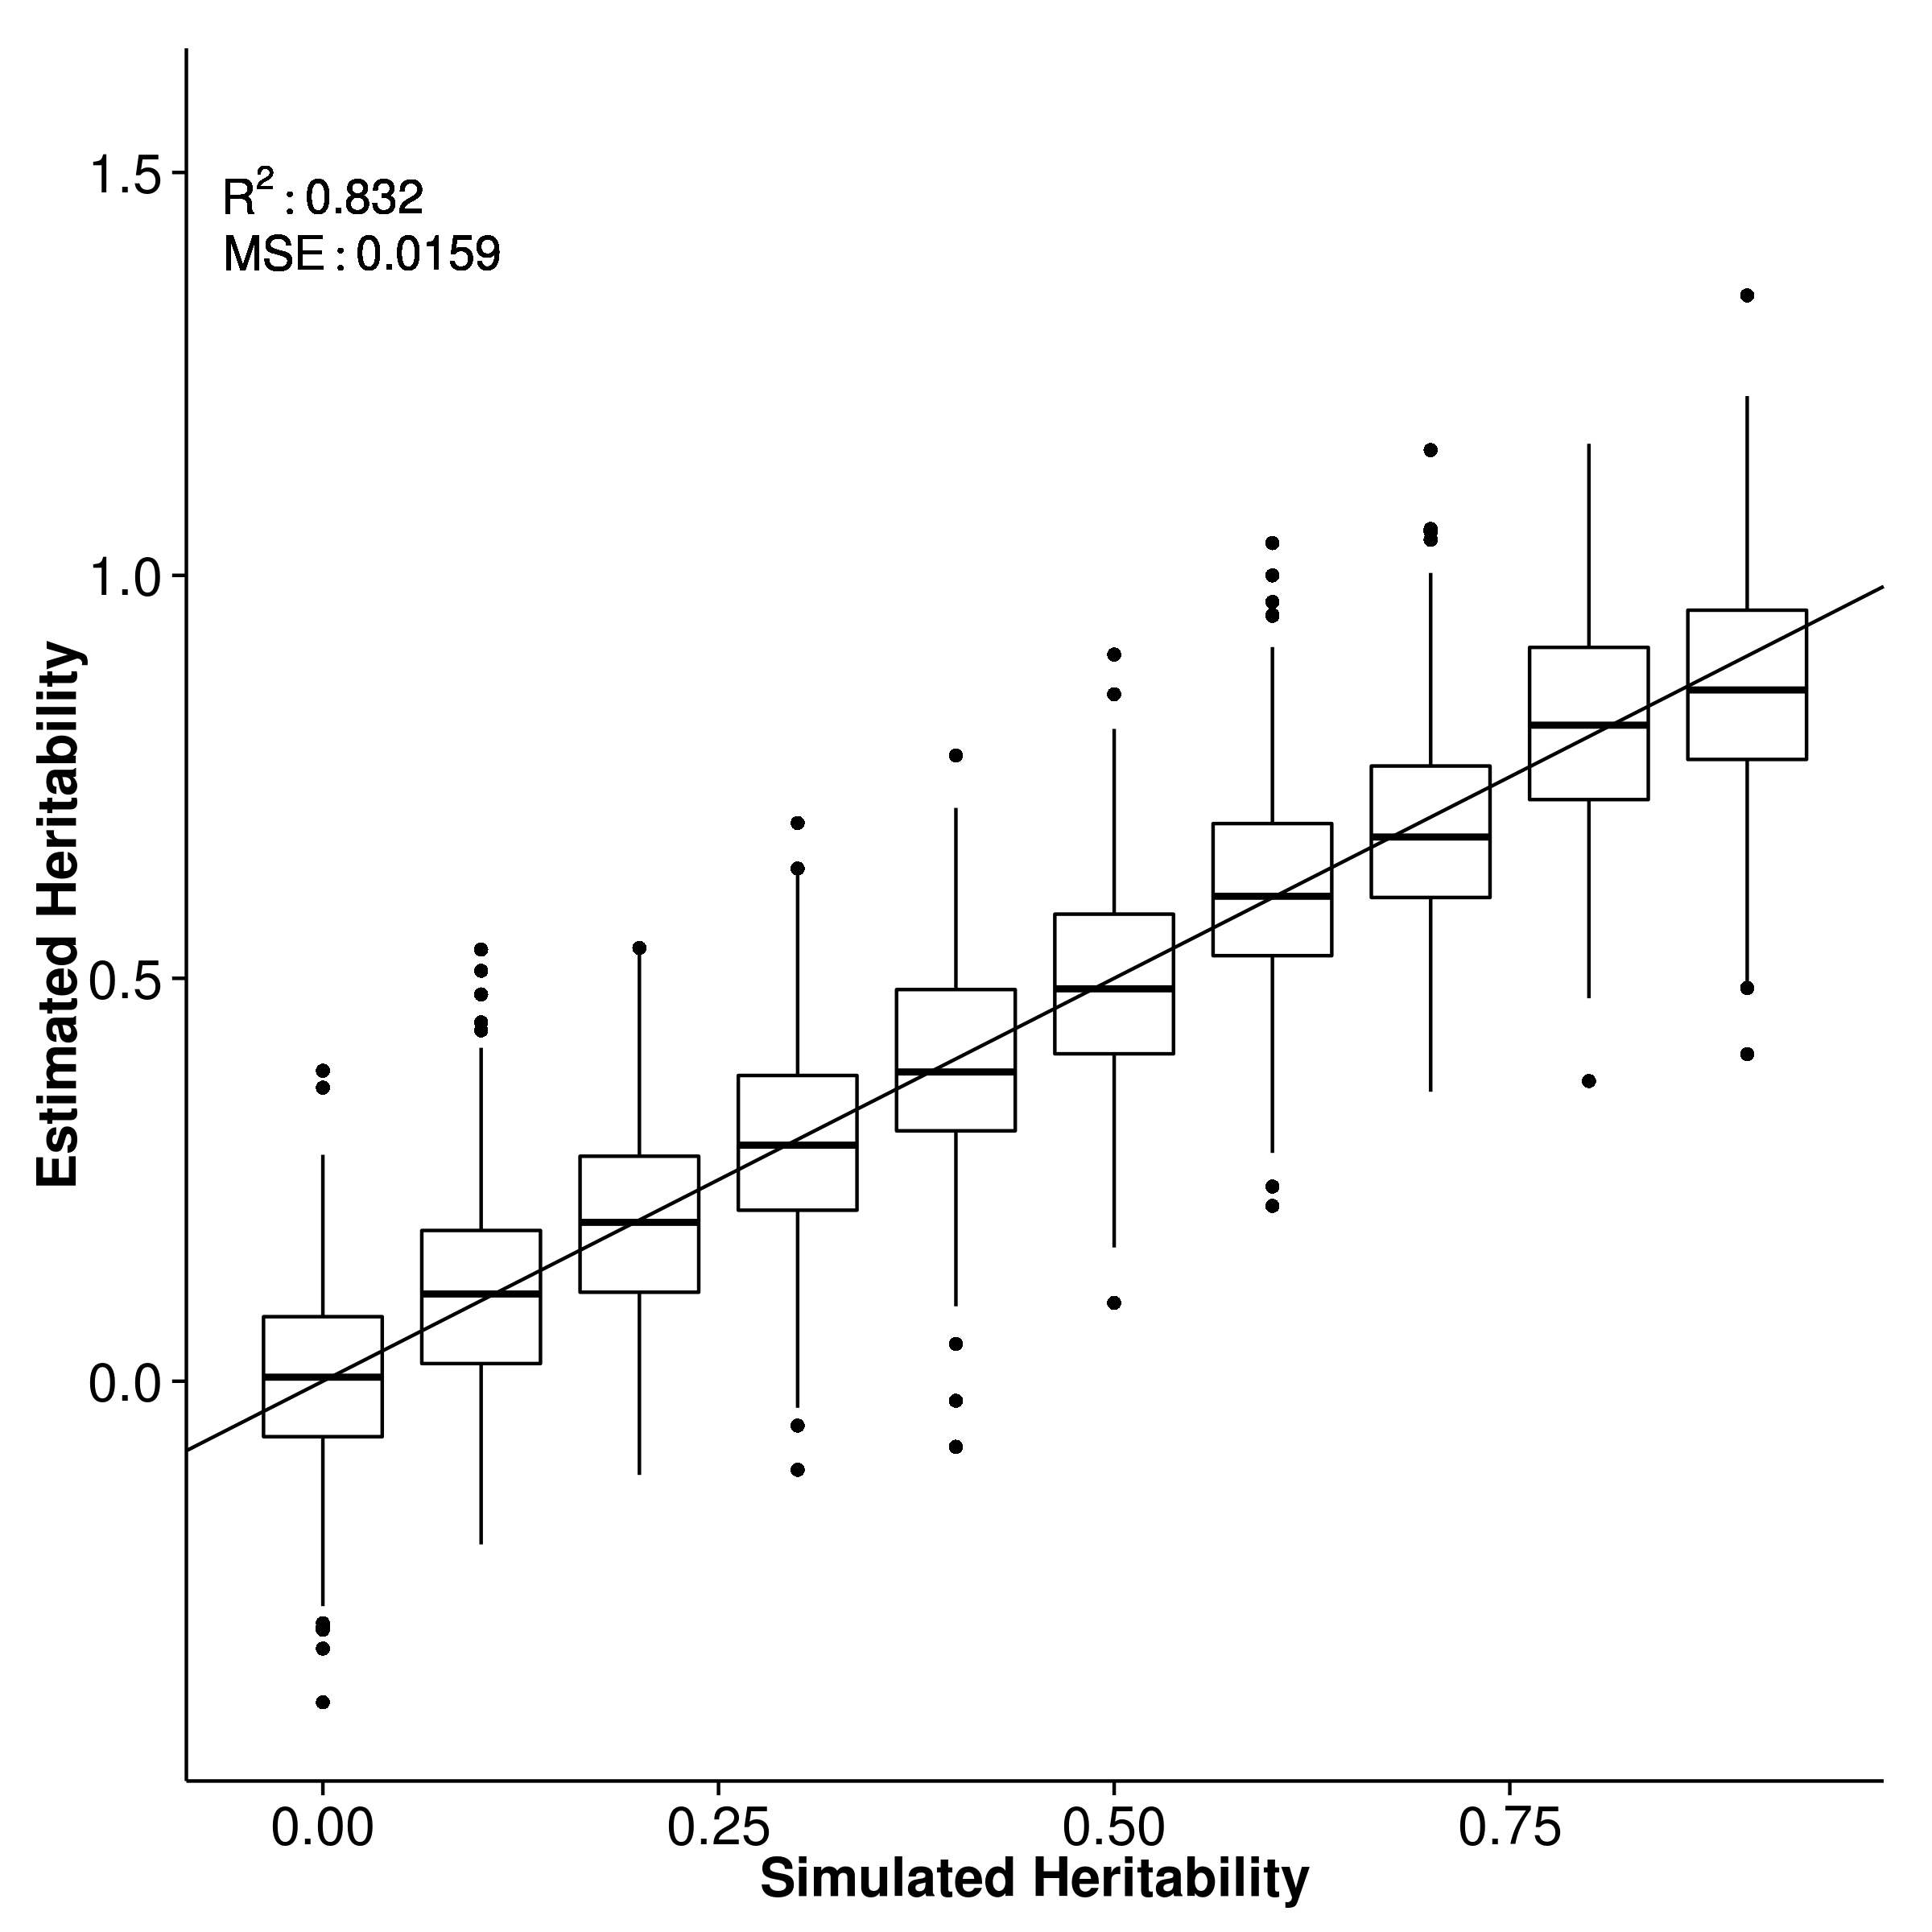
\includegraphics{figure/quantitative/random_effect/10c/shrek_50k_10c_meanH.png}}
				\label{fig:50k10cQtmeanSre}
			}
			\subfloat[GCTA]{
				\scalebox{.4}{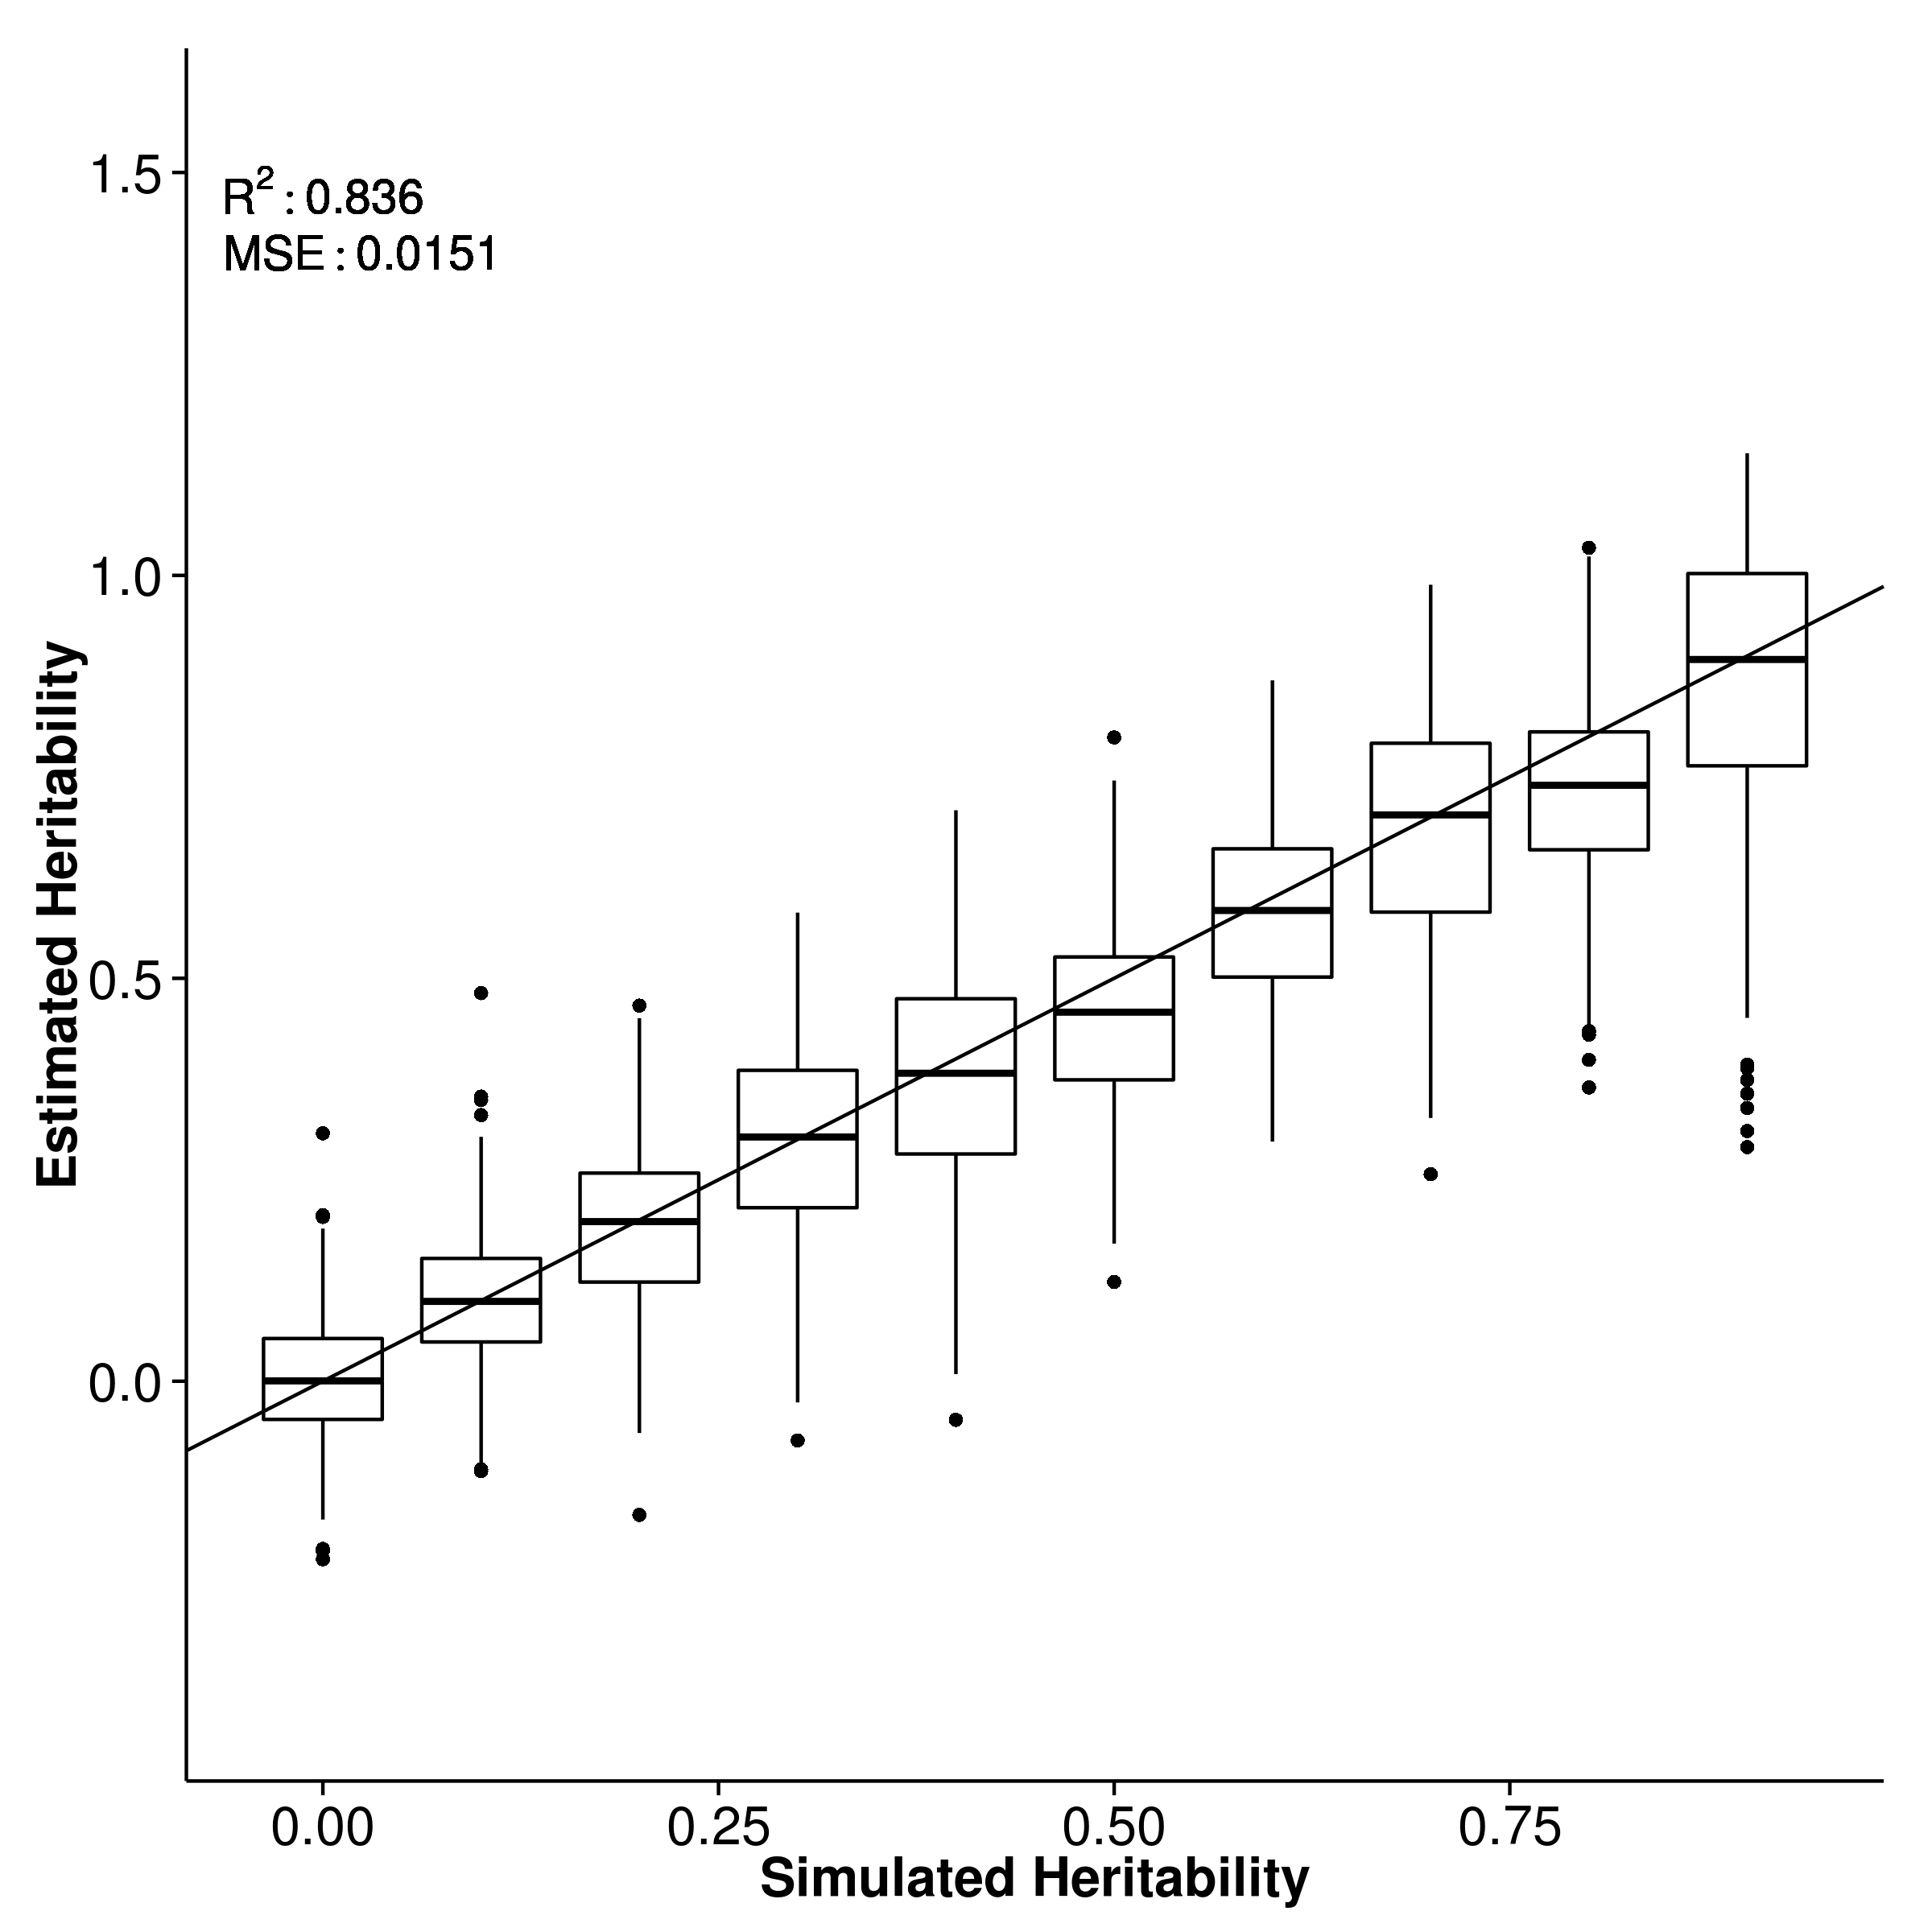
\includegraphics{figure/quantitative/random_effect/10c/gcta_50k_10c_meanH.png}}
				\label{fig:50k10cQtmeanGre}
			}\\
			\subfloat[LDSC with fix intercept]{
				\scalebox{.4}{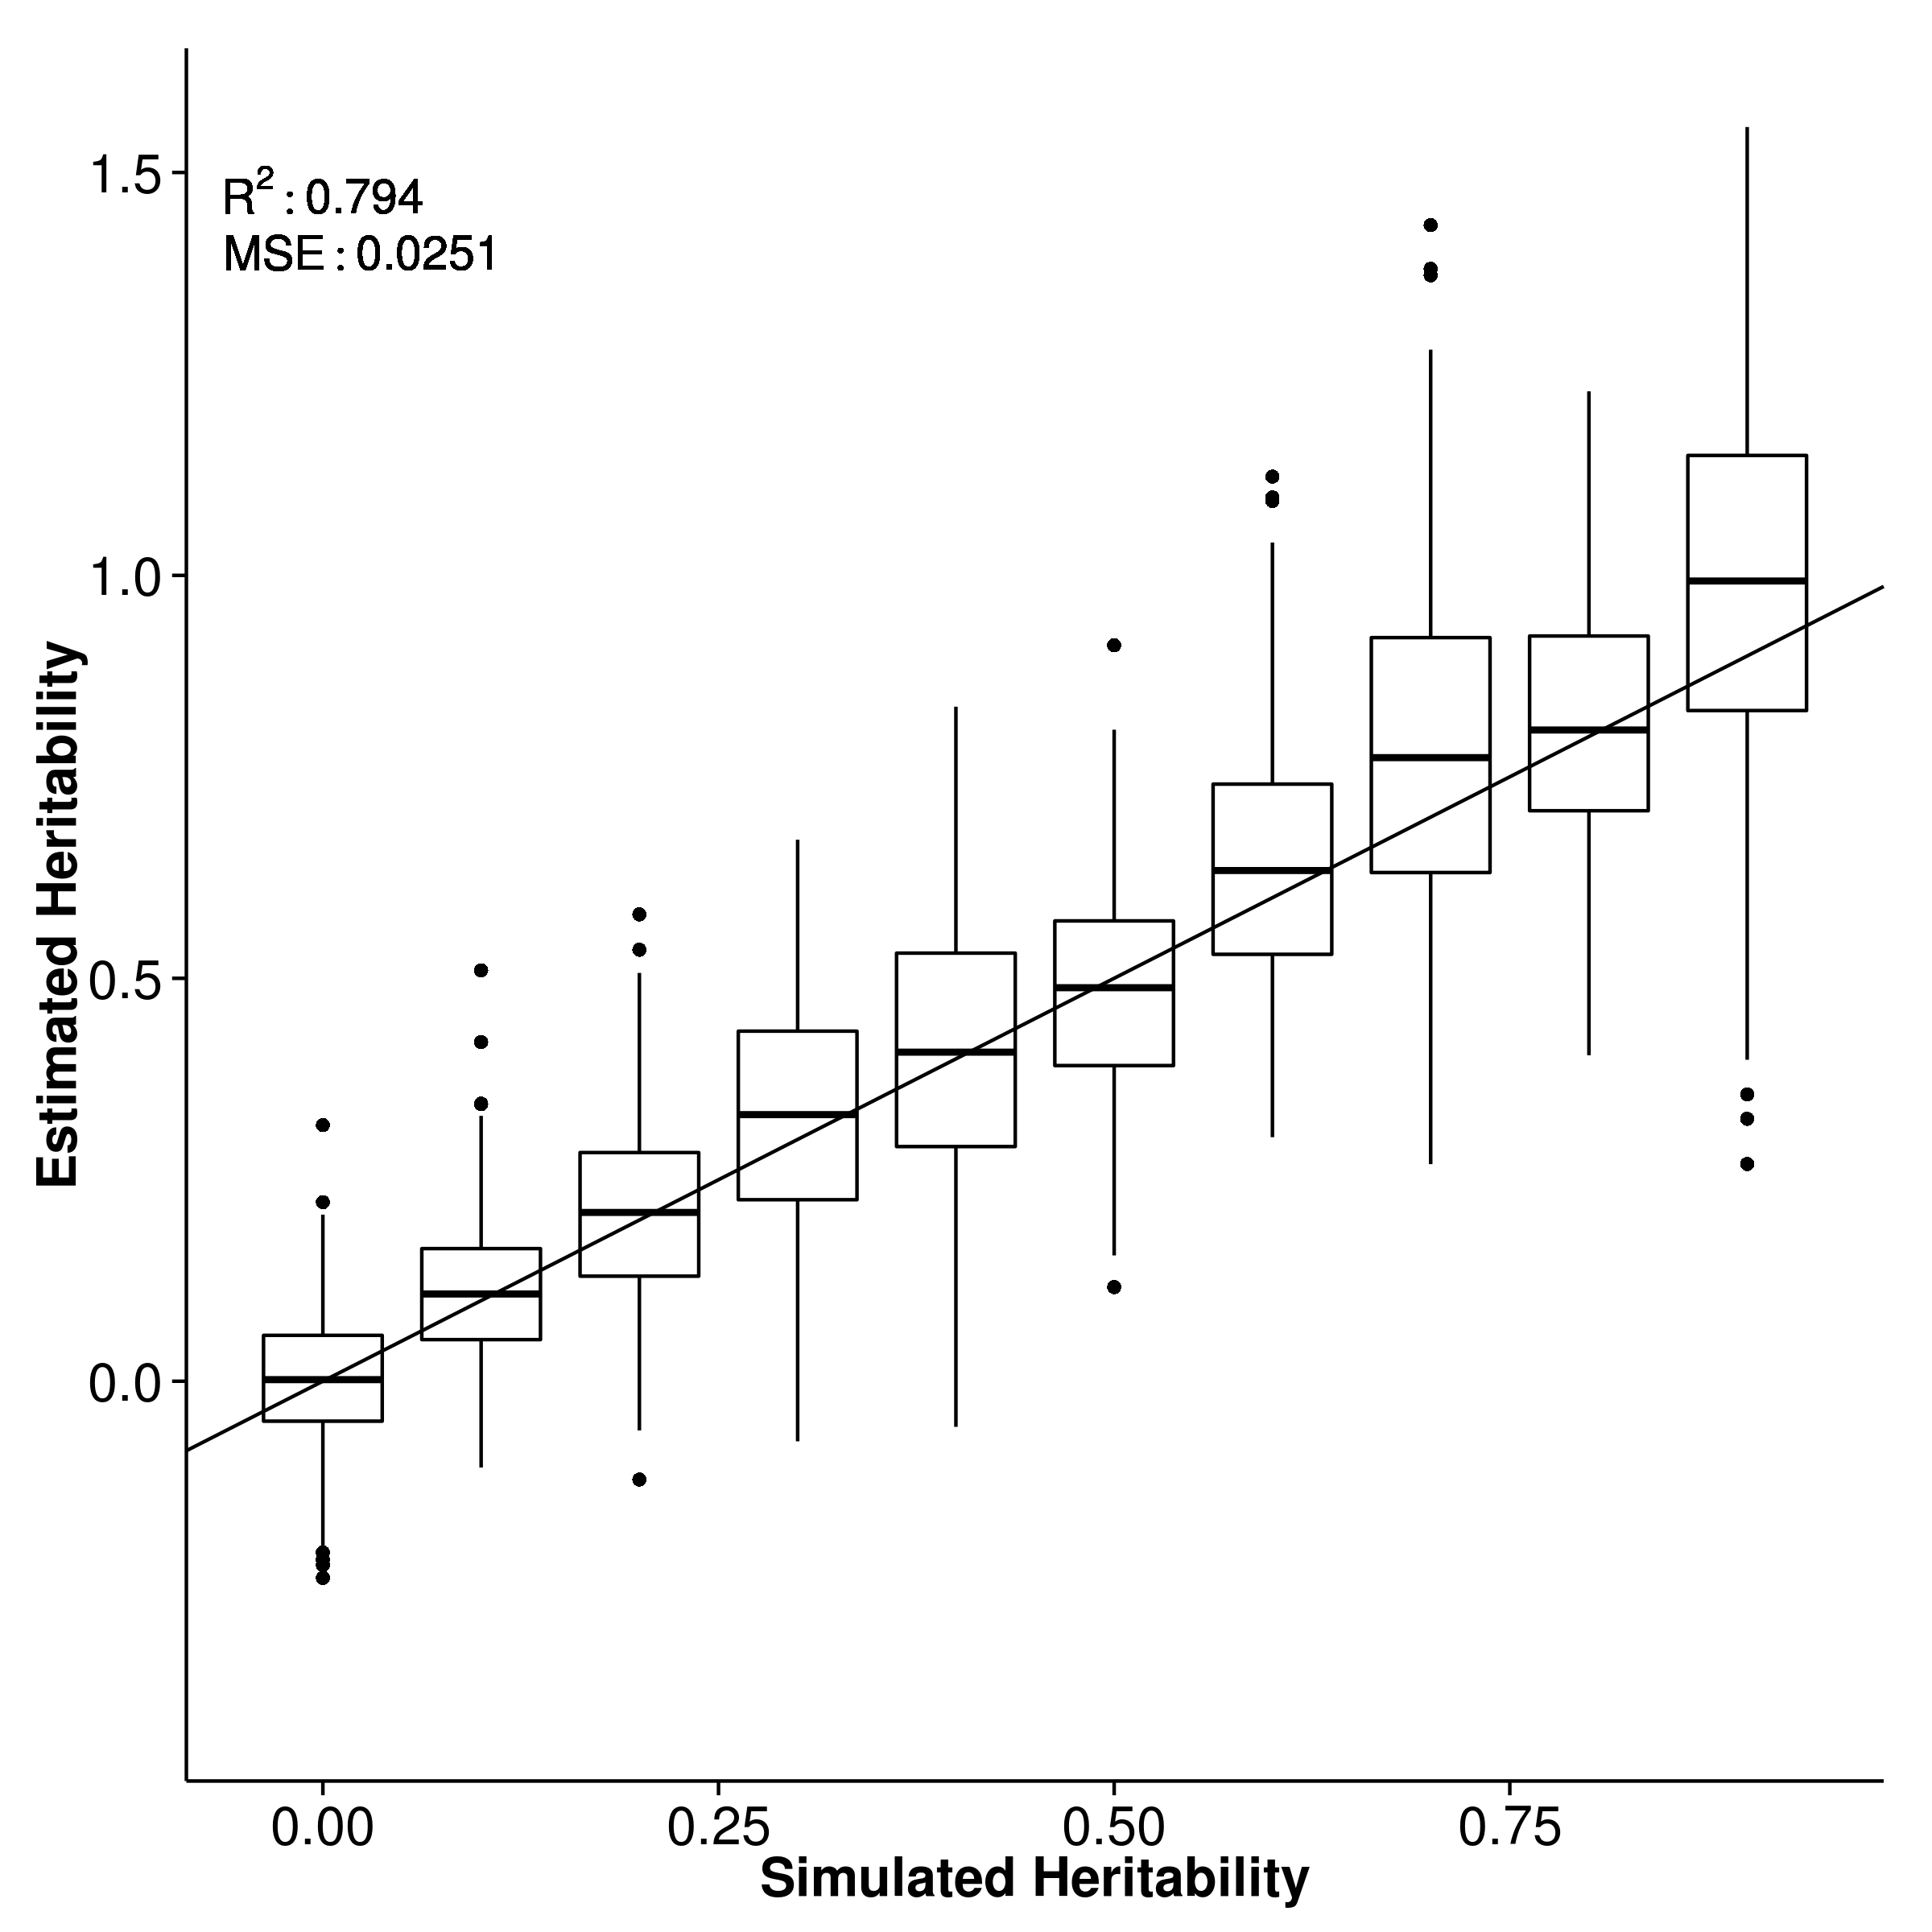
\includegraphics{figure/quantitative/random_effect/10c/ldsc_50k_10c_meanH.png}}
				\label{fig:50k10cQtmeanLre}
			}
			\subfloat[LDSC with intercept estimation]{
				\scalebox{.4}{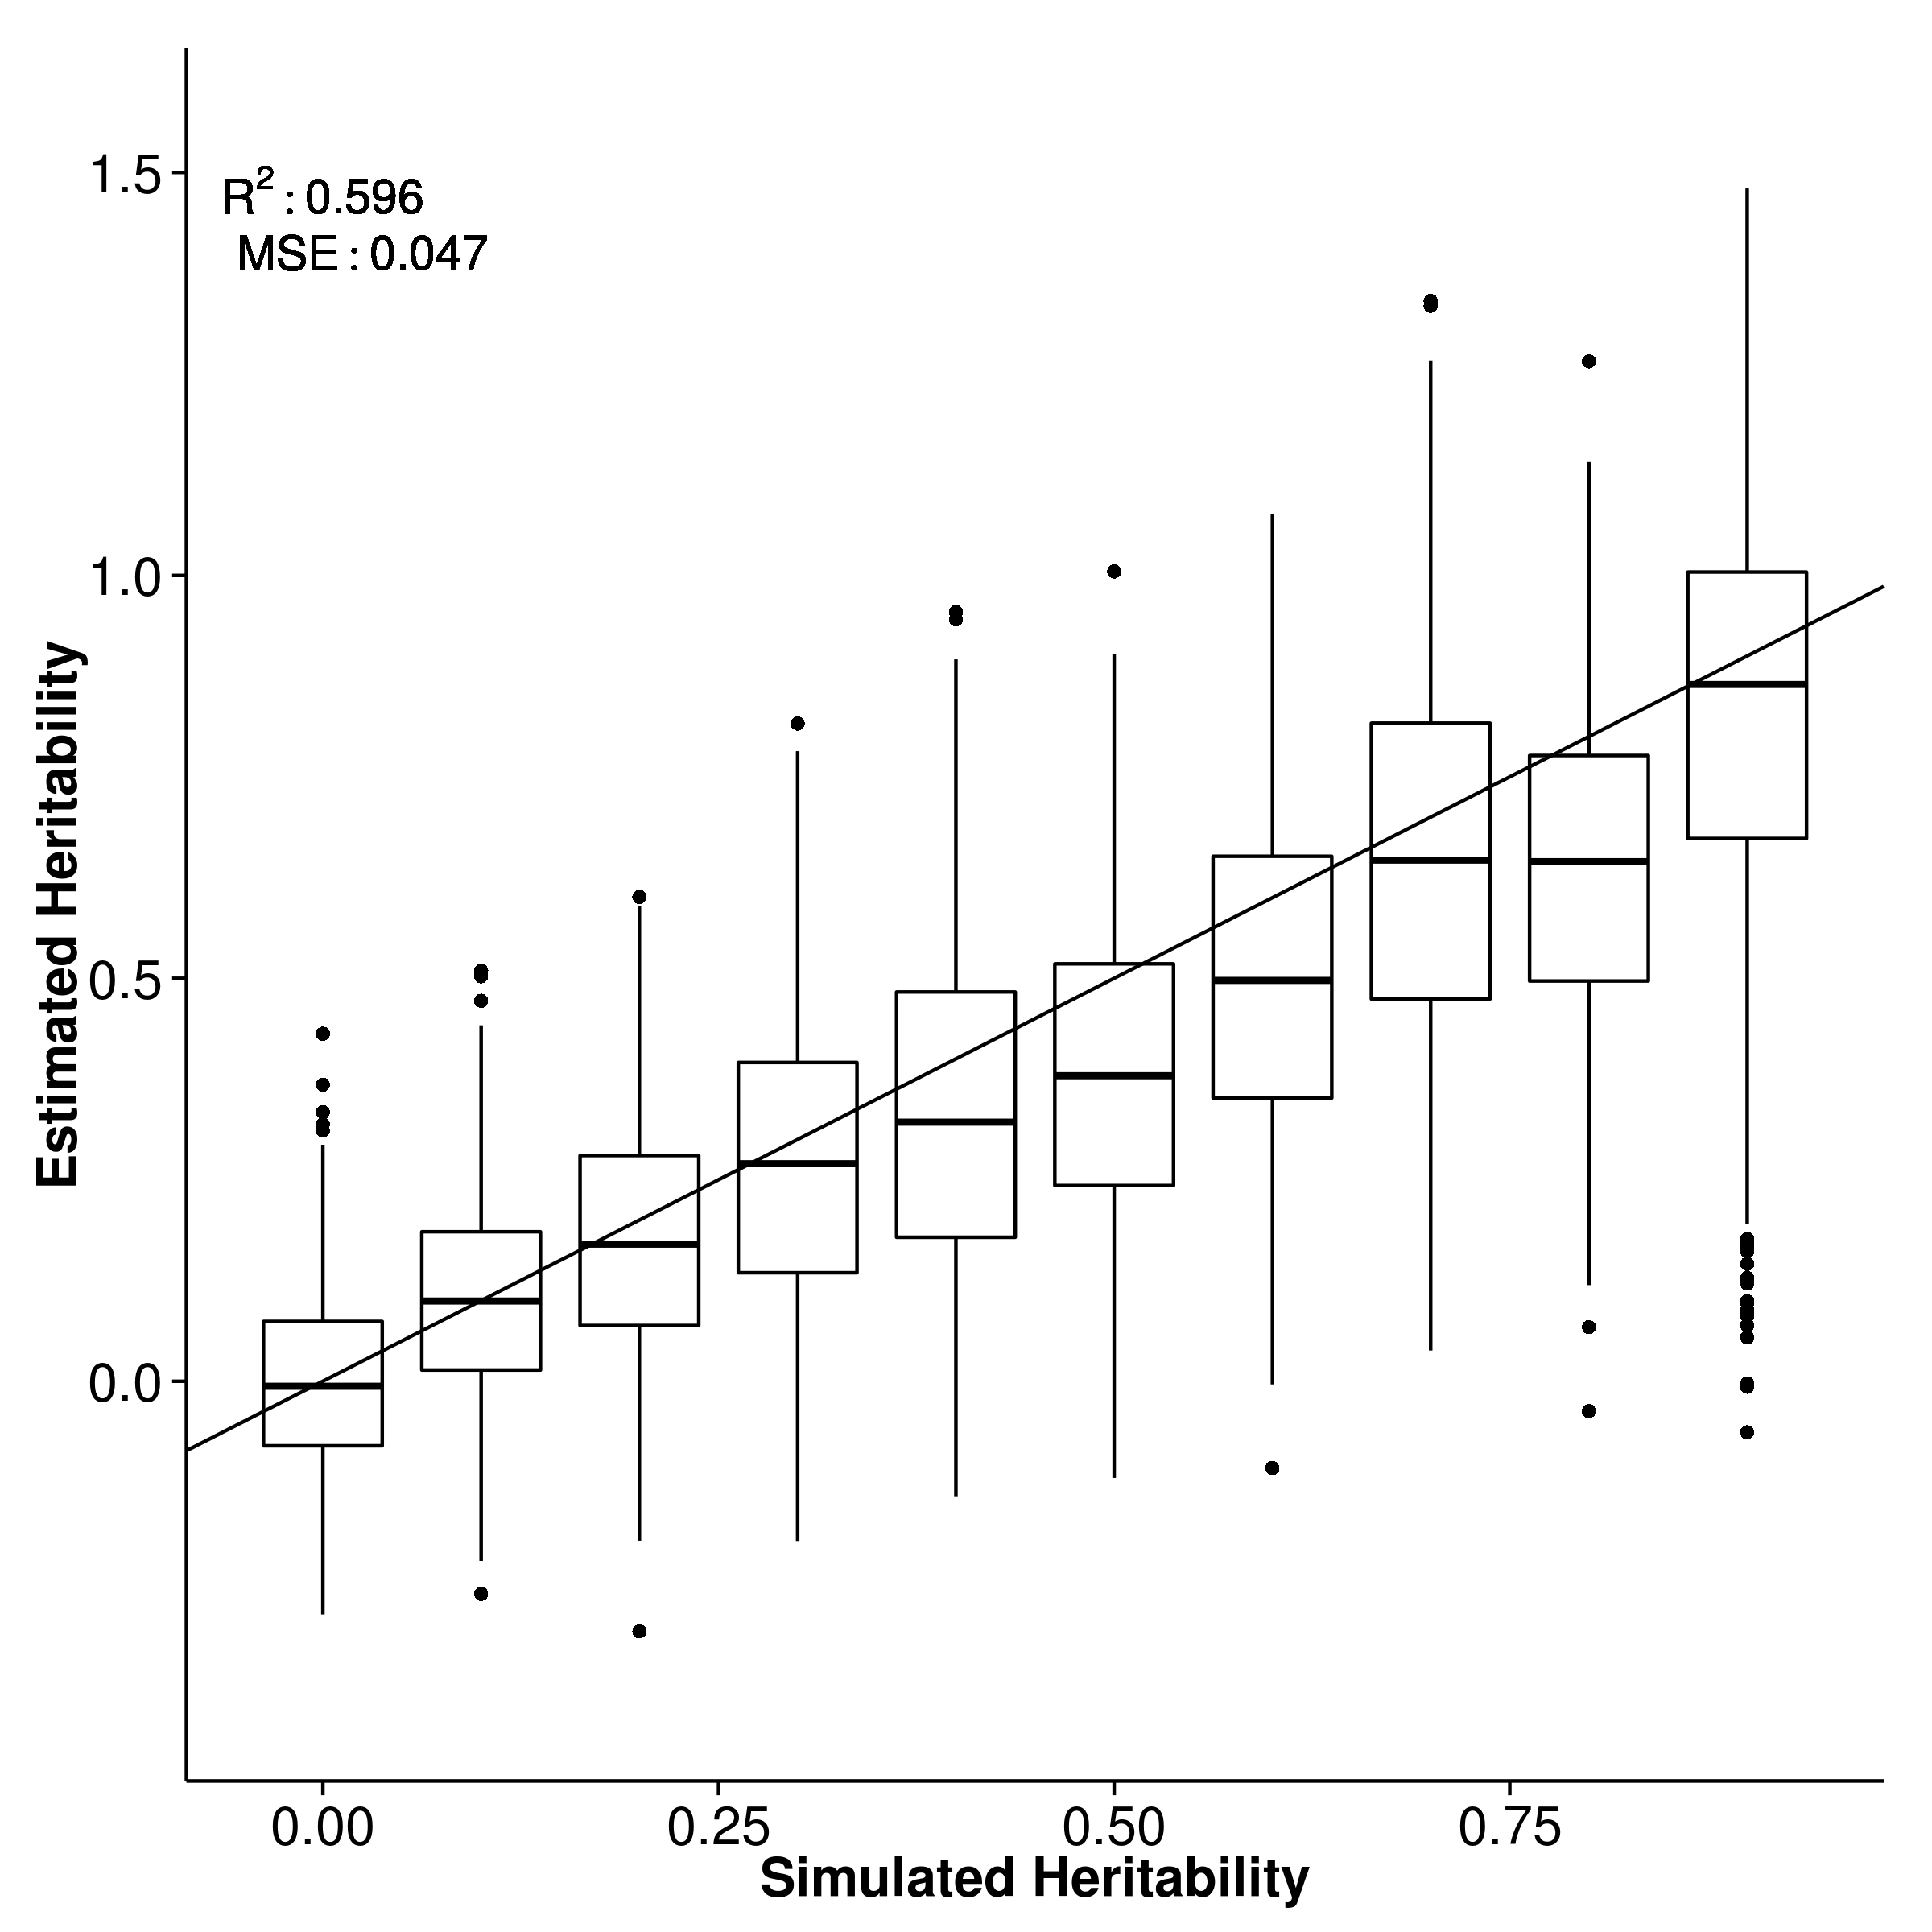
\includegraphics{figure/quantitative/random_effect/10c/ldscIn_50k_10c_meanH.png}}
				\label{fig:50k10cQtmeanIre}
			}
			\caption[Simulation of Quantitative Traits with 50k \glsentryshortpl{SNP} and 10 causal variants of random effect size]
			{Simulation of Quantitative Traits with 50k \glsentryshortpl{SNP} and 10 causal variants with random effect size.} 
			\label{fig:50k10cQtMeanre}
		\end{figure}
		\begin{figure}
			\centering
			\centering
			\subfloat[SHREK]{
				\scalebox{.4}{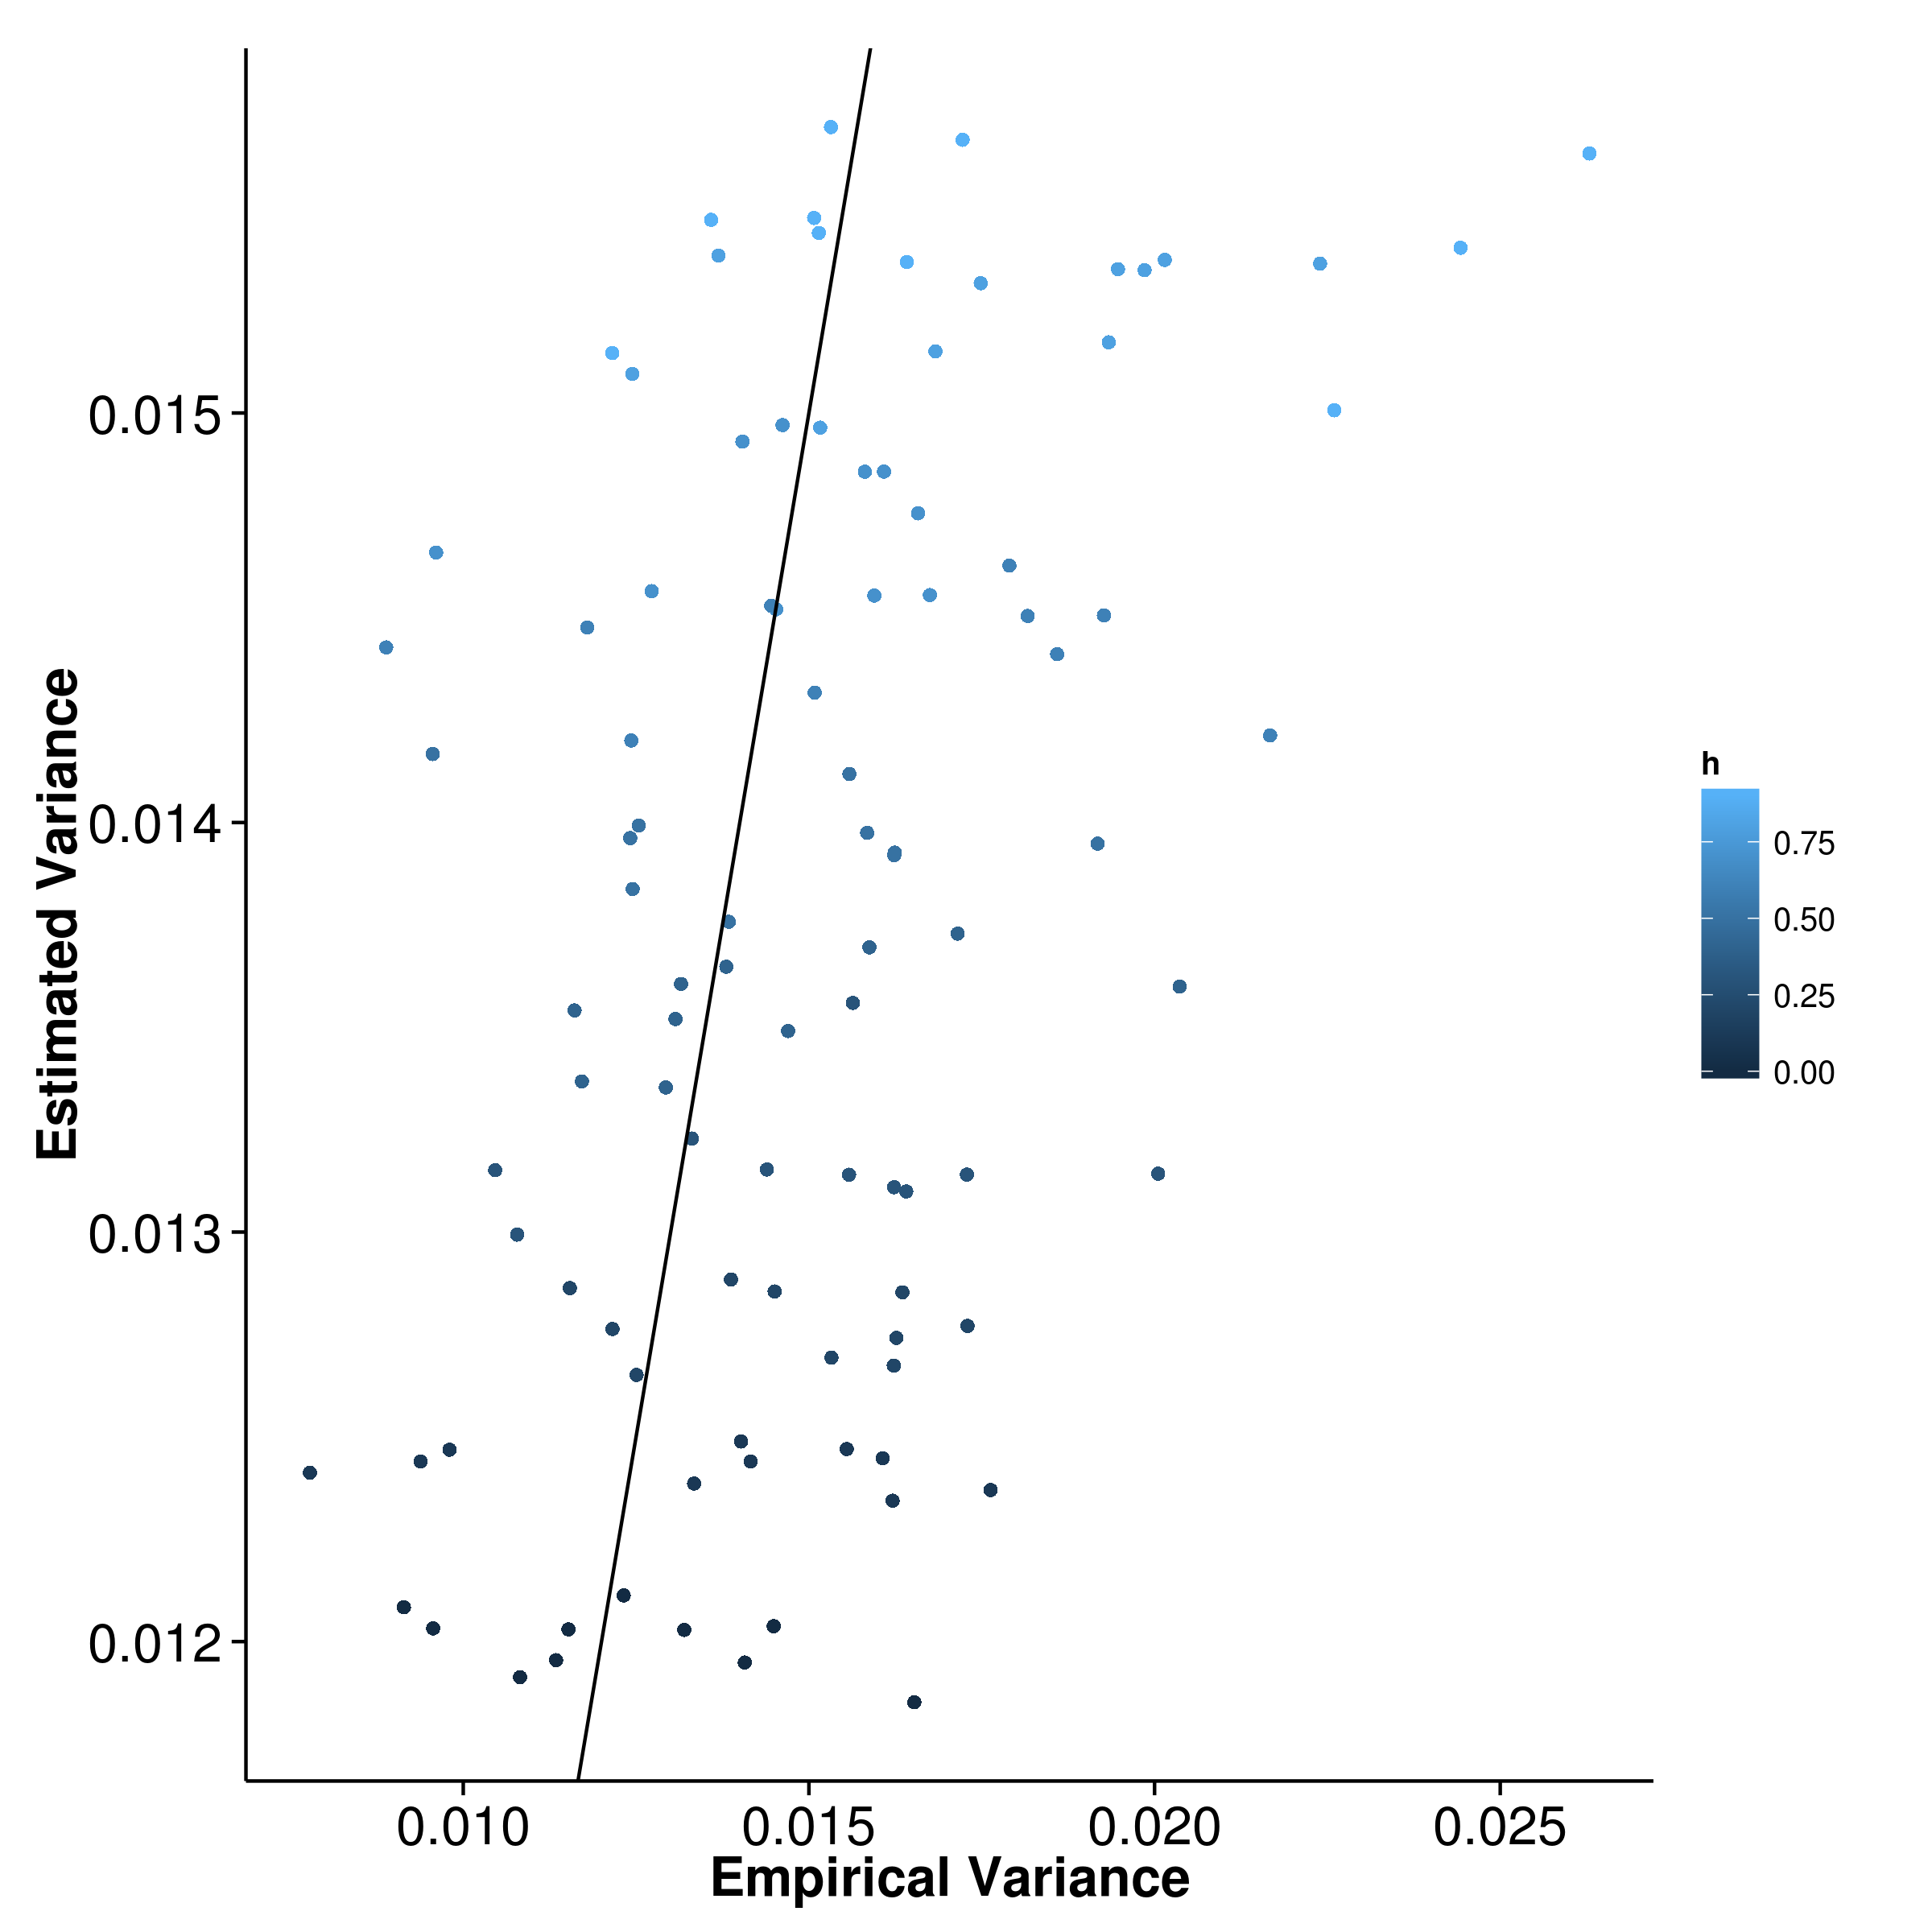
\includegraphics{figure/quantitative/random_effect/10c/shrek_50k_10c_varH.png}}
				\label{fig:50k10cQtvarSre}
			}
			\subfloat[GCTA]{
				\scalebox{.4}{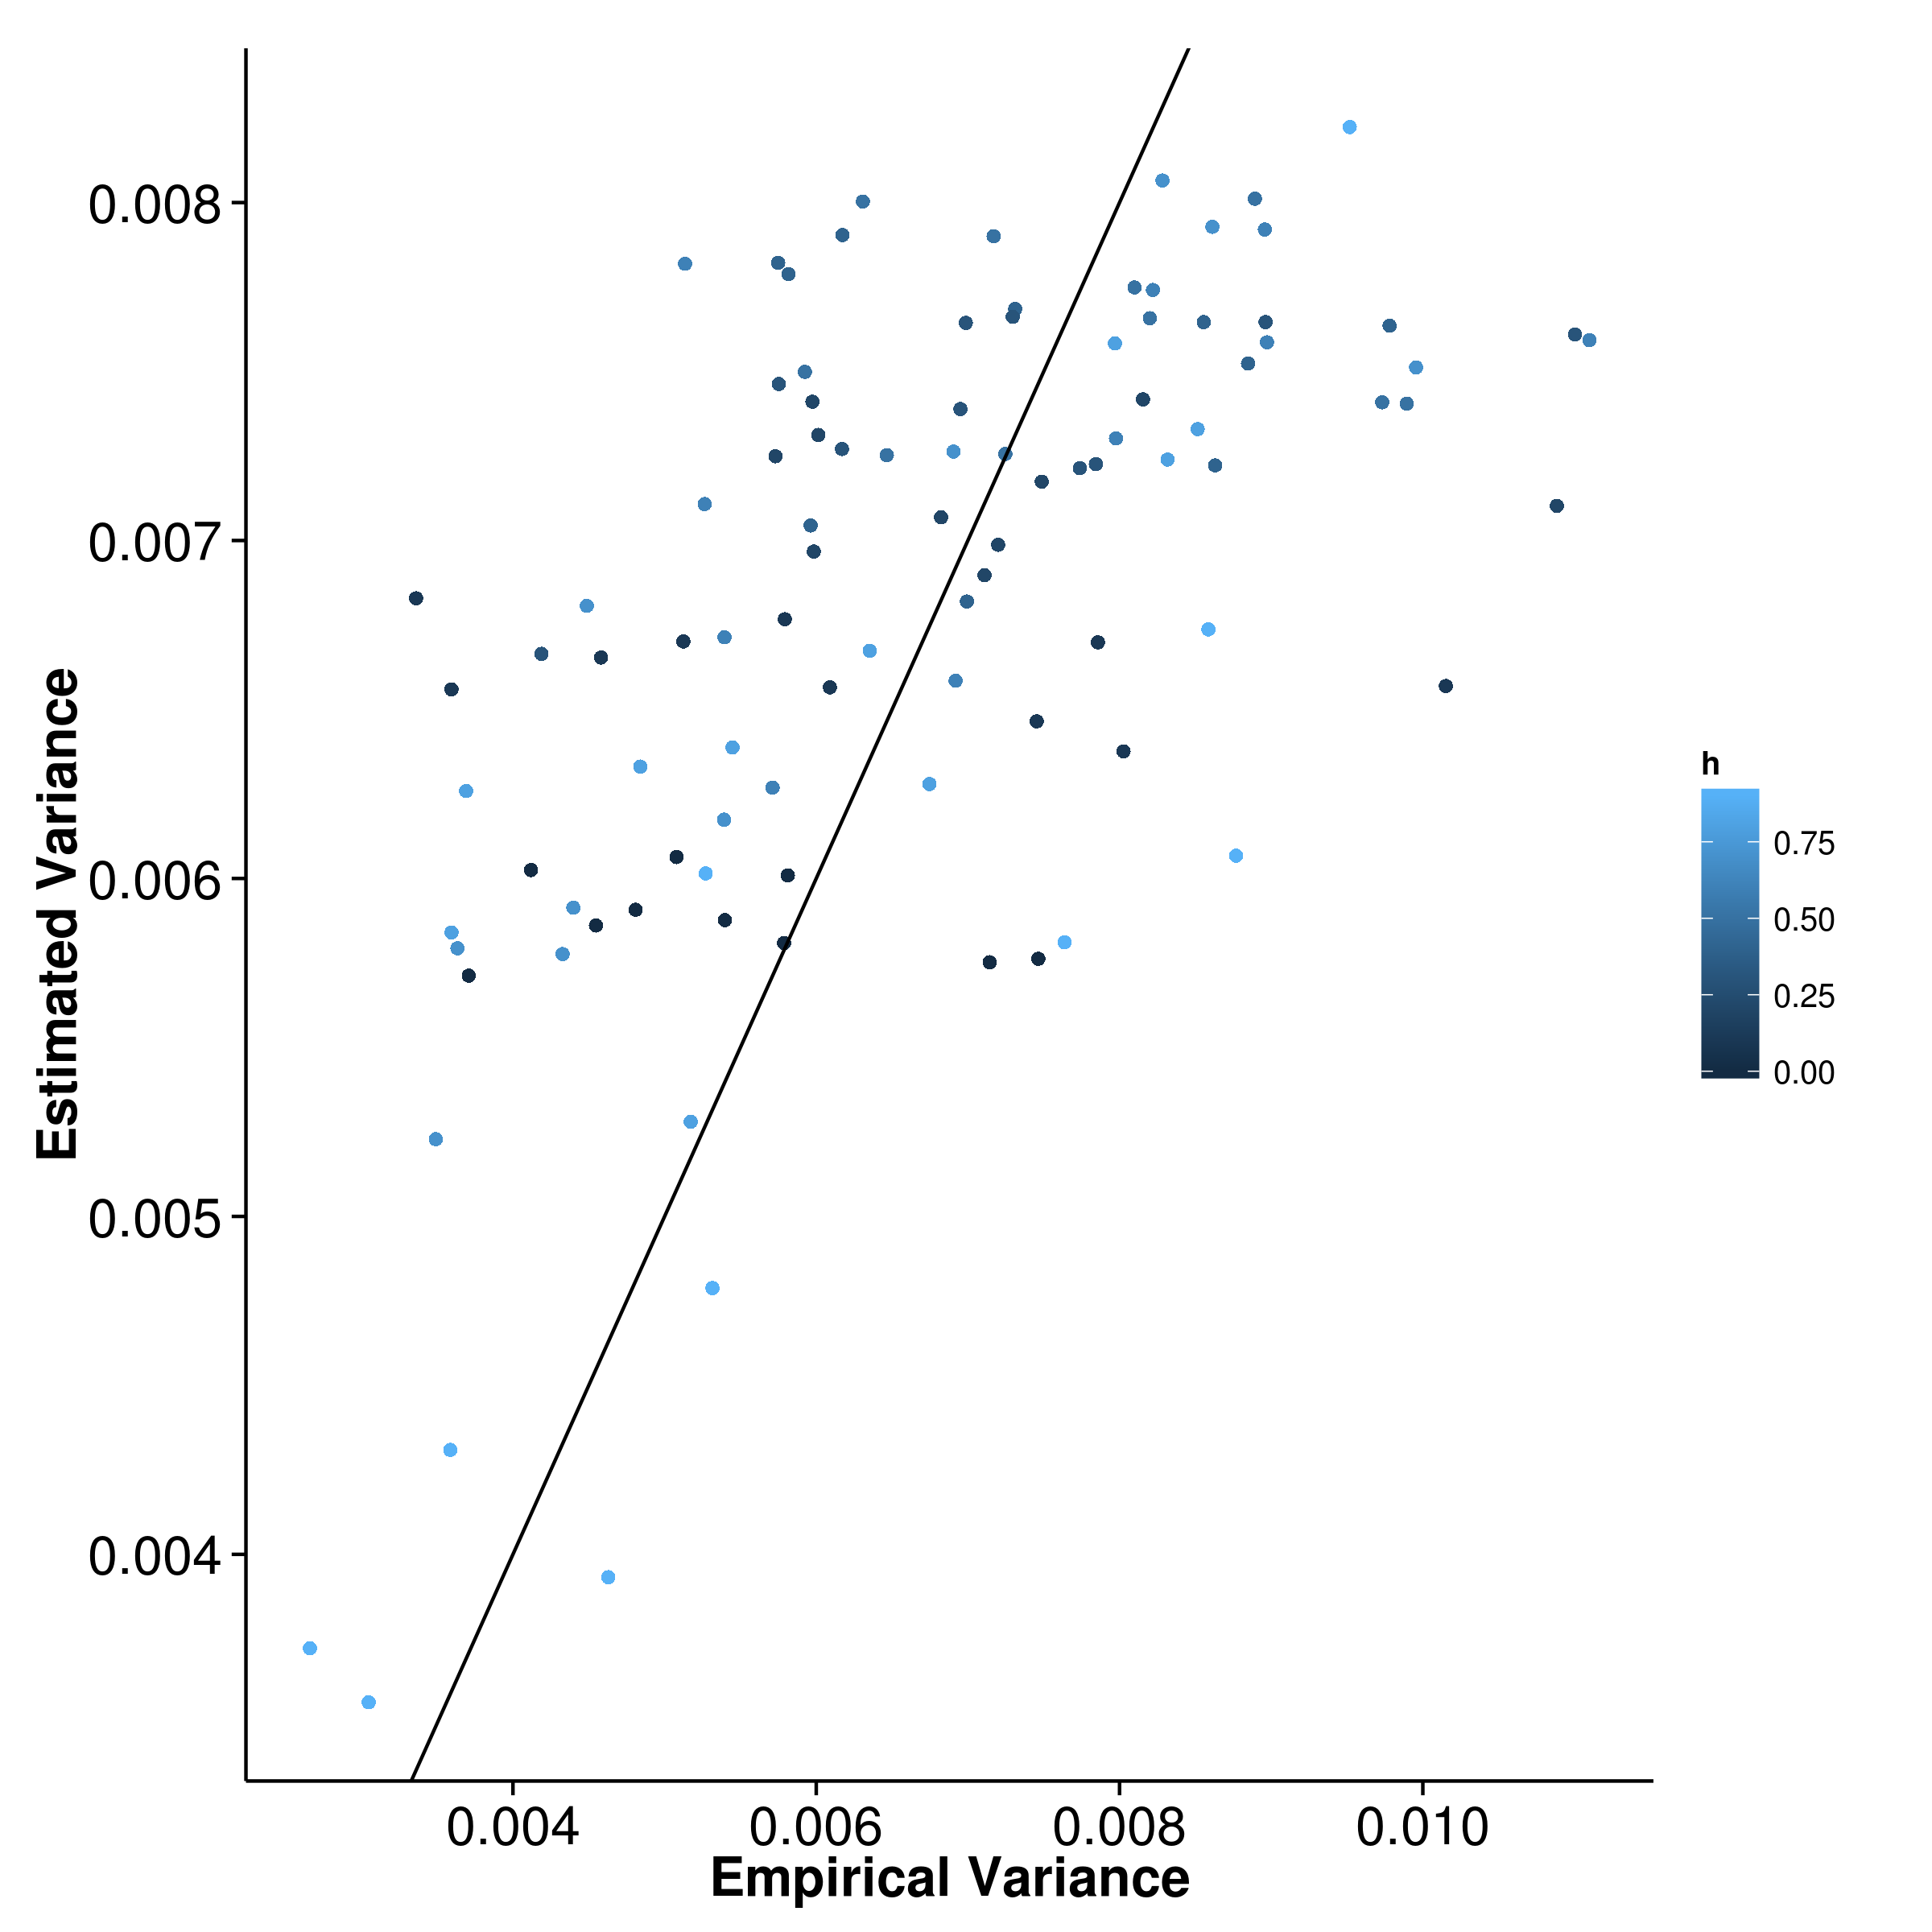
\includegraphics{figure/quantitative/random_effect/10c/gcta_50k_10c_varH.png}}
				\label{fig:50k10cQtvarGre}
			}\\
			\subfloat[LDSC with fix intercept]{
				\scalebox{.4}{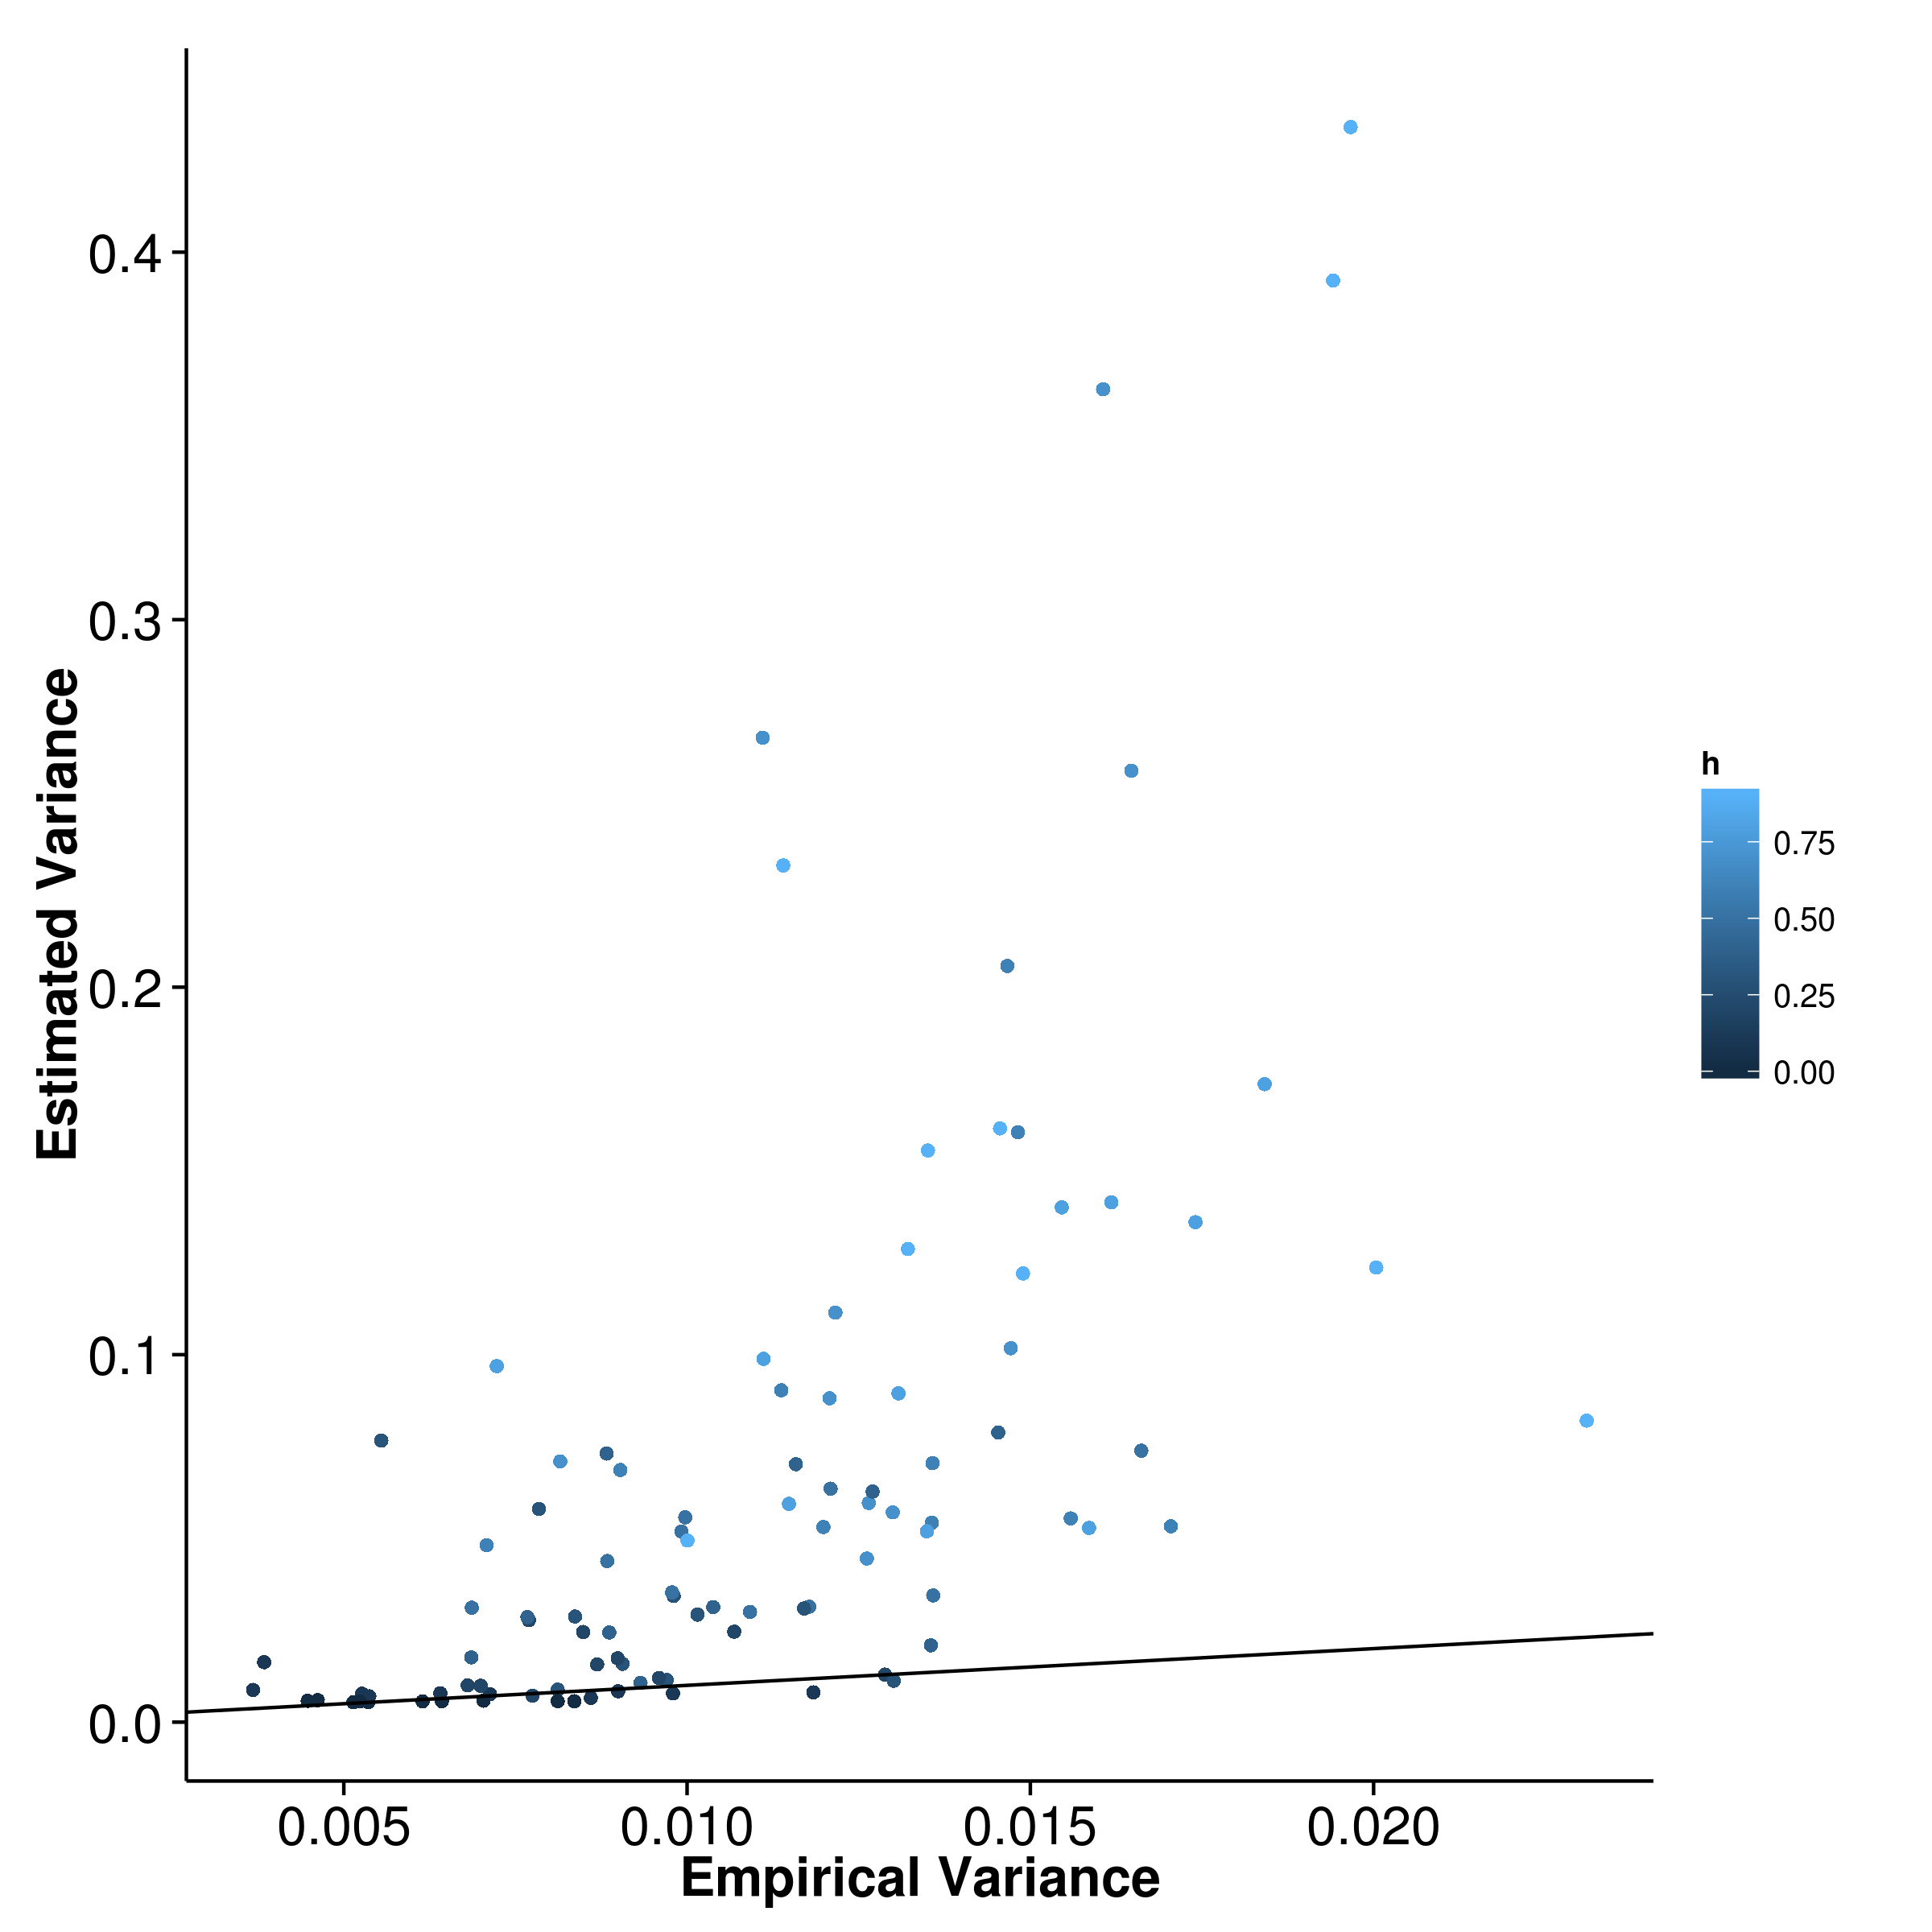
\includegraphics{figure/quantitative/random_effect/10c/ldsc_50k_10c_varH.png}}
				\label{fig:50k10cQtvarLre}
			}
			\subfloat[LDSC with intercept estimation]{
				\scalebox{.4}{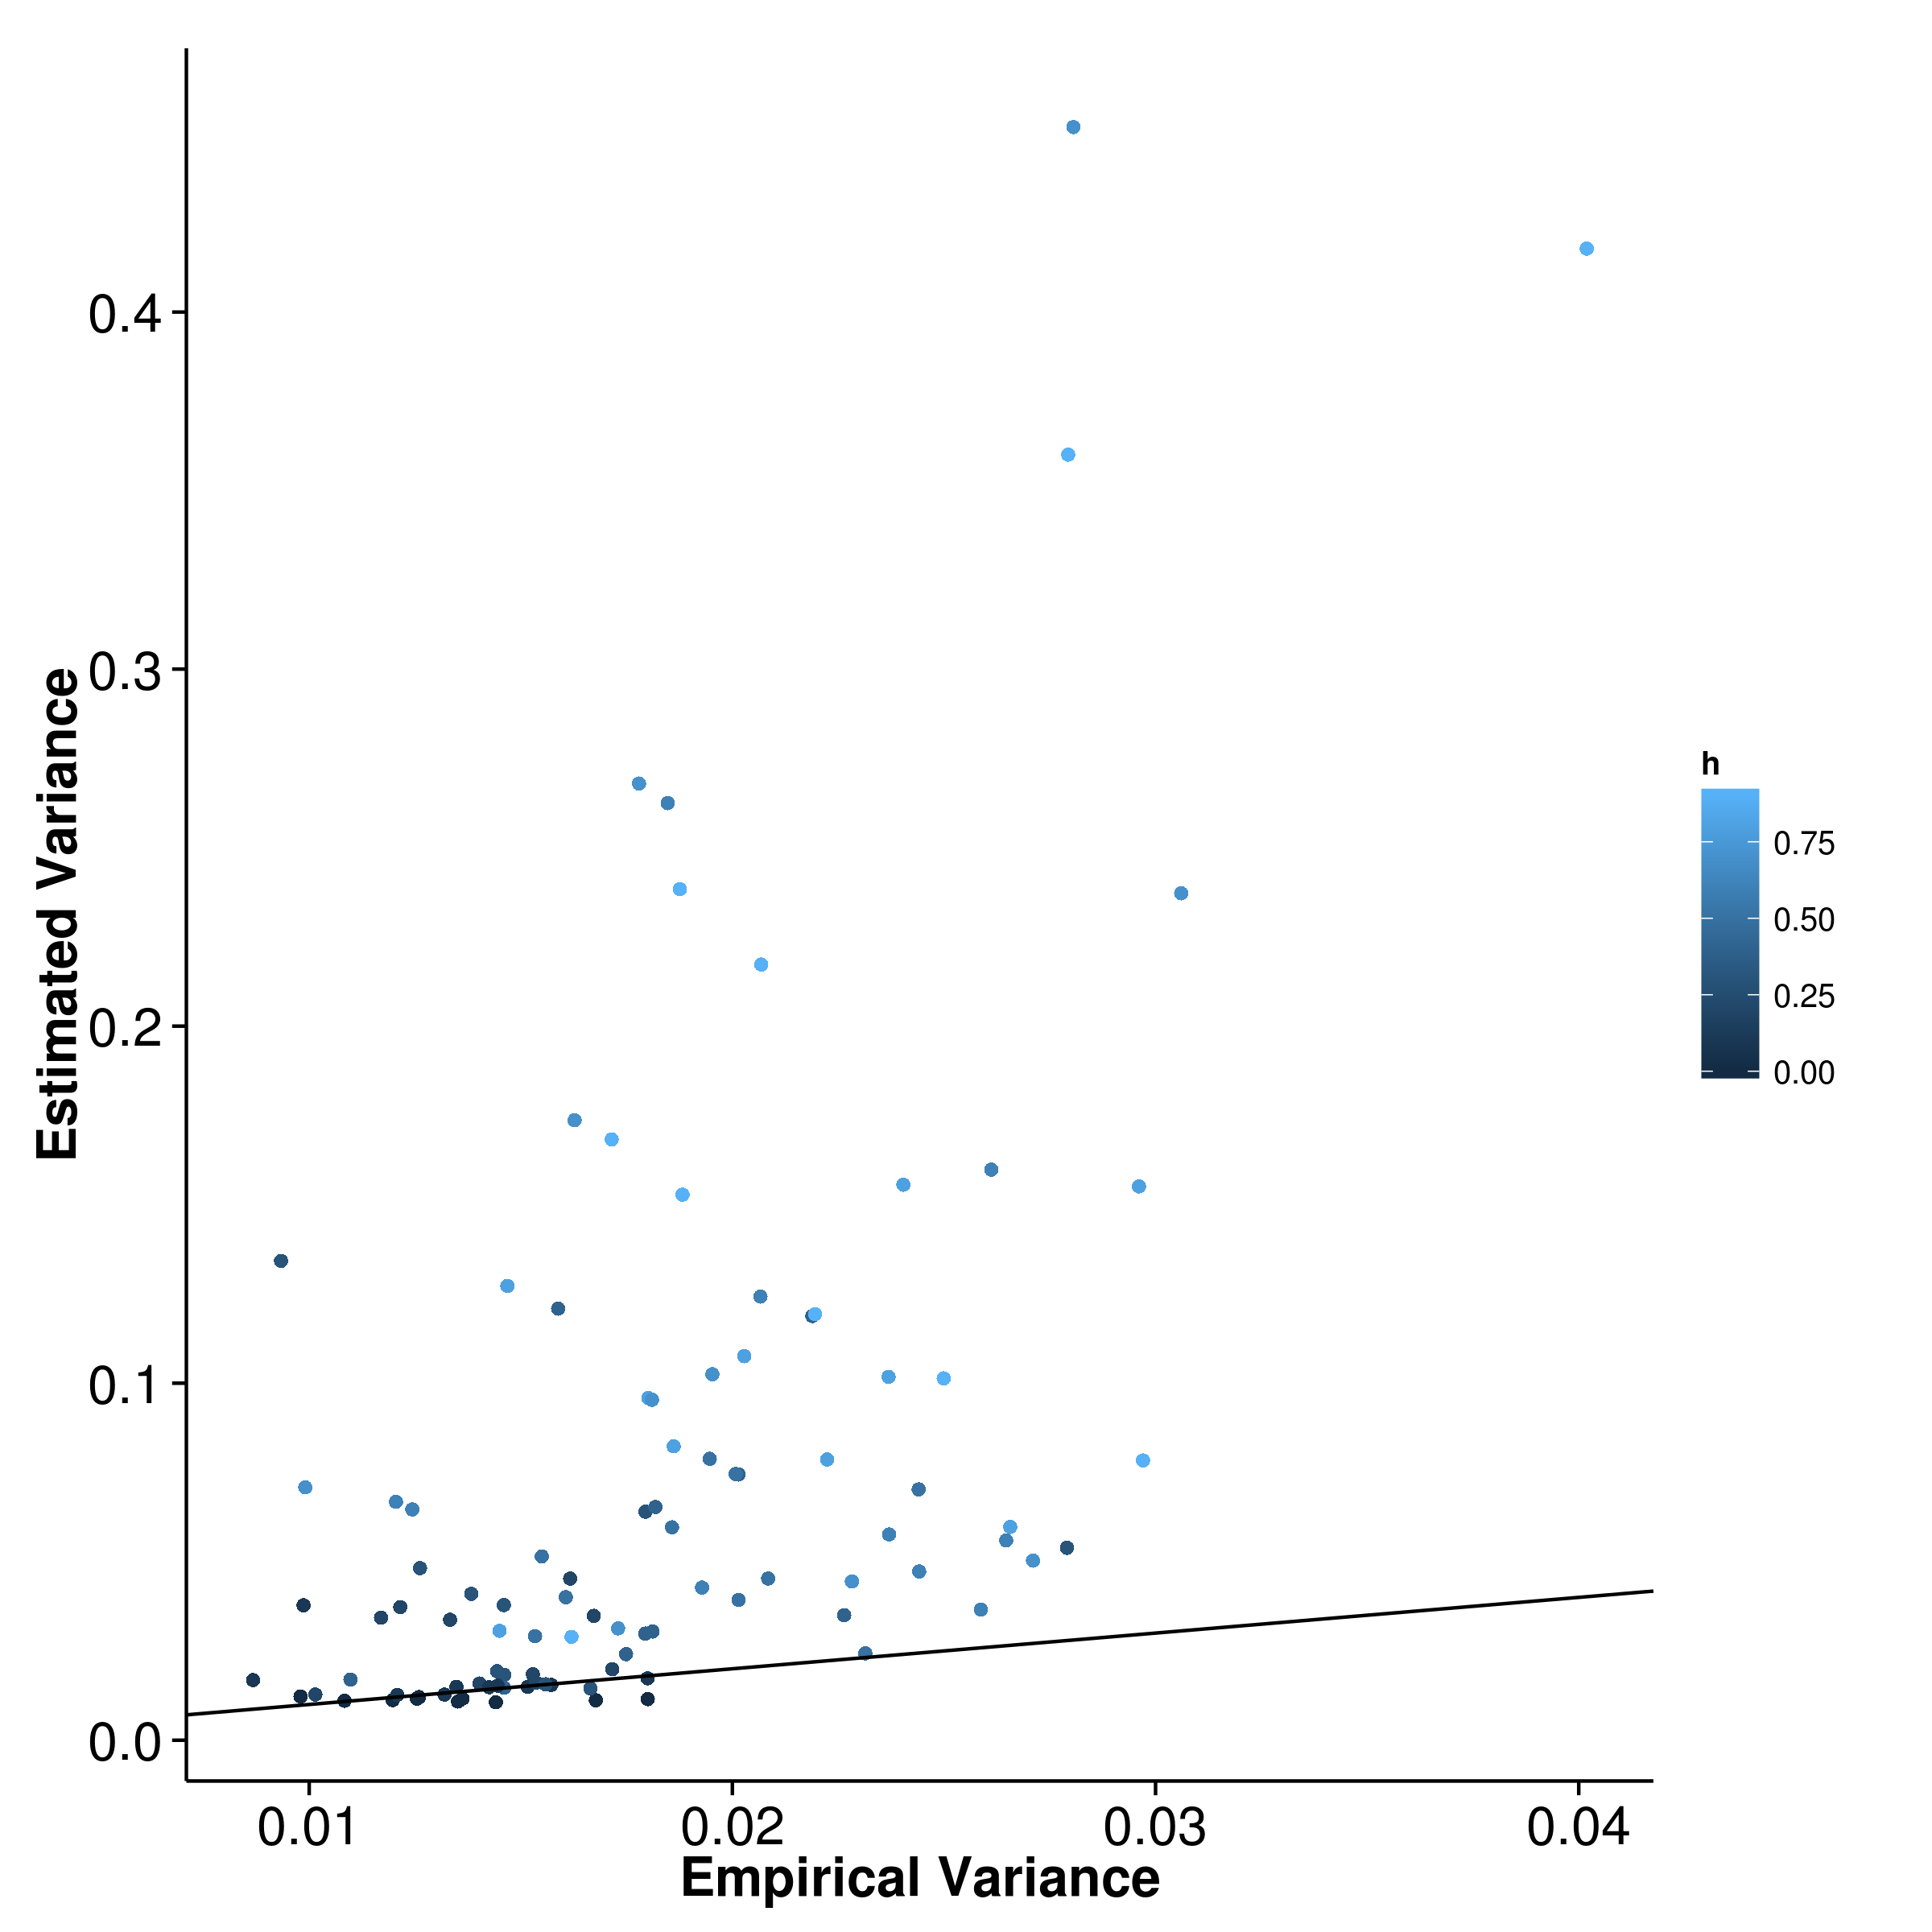
\includegraphics{figure/quantitative/random_effect/10c/ldscIn_50k_10c_varH.png}}
				\label{fig:50k10cQtvarIre}
			}
			\label{fig:50k10cQtVarre}
		\end{figure}
		
		
		
		\begin{figure}
			\centering
			\centering
			\subfloat[SHREK]{
				\scalebox{.4}{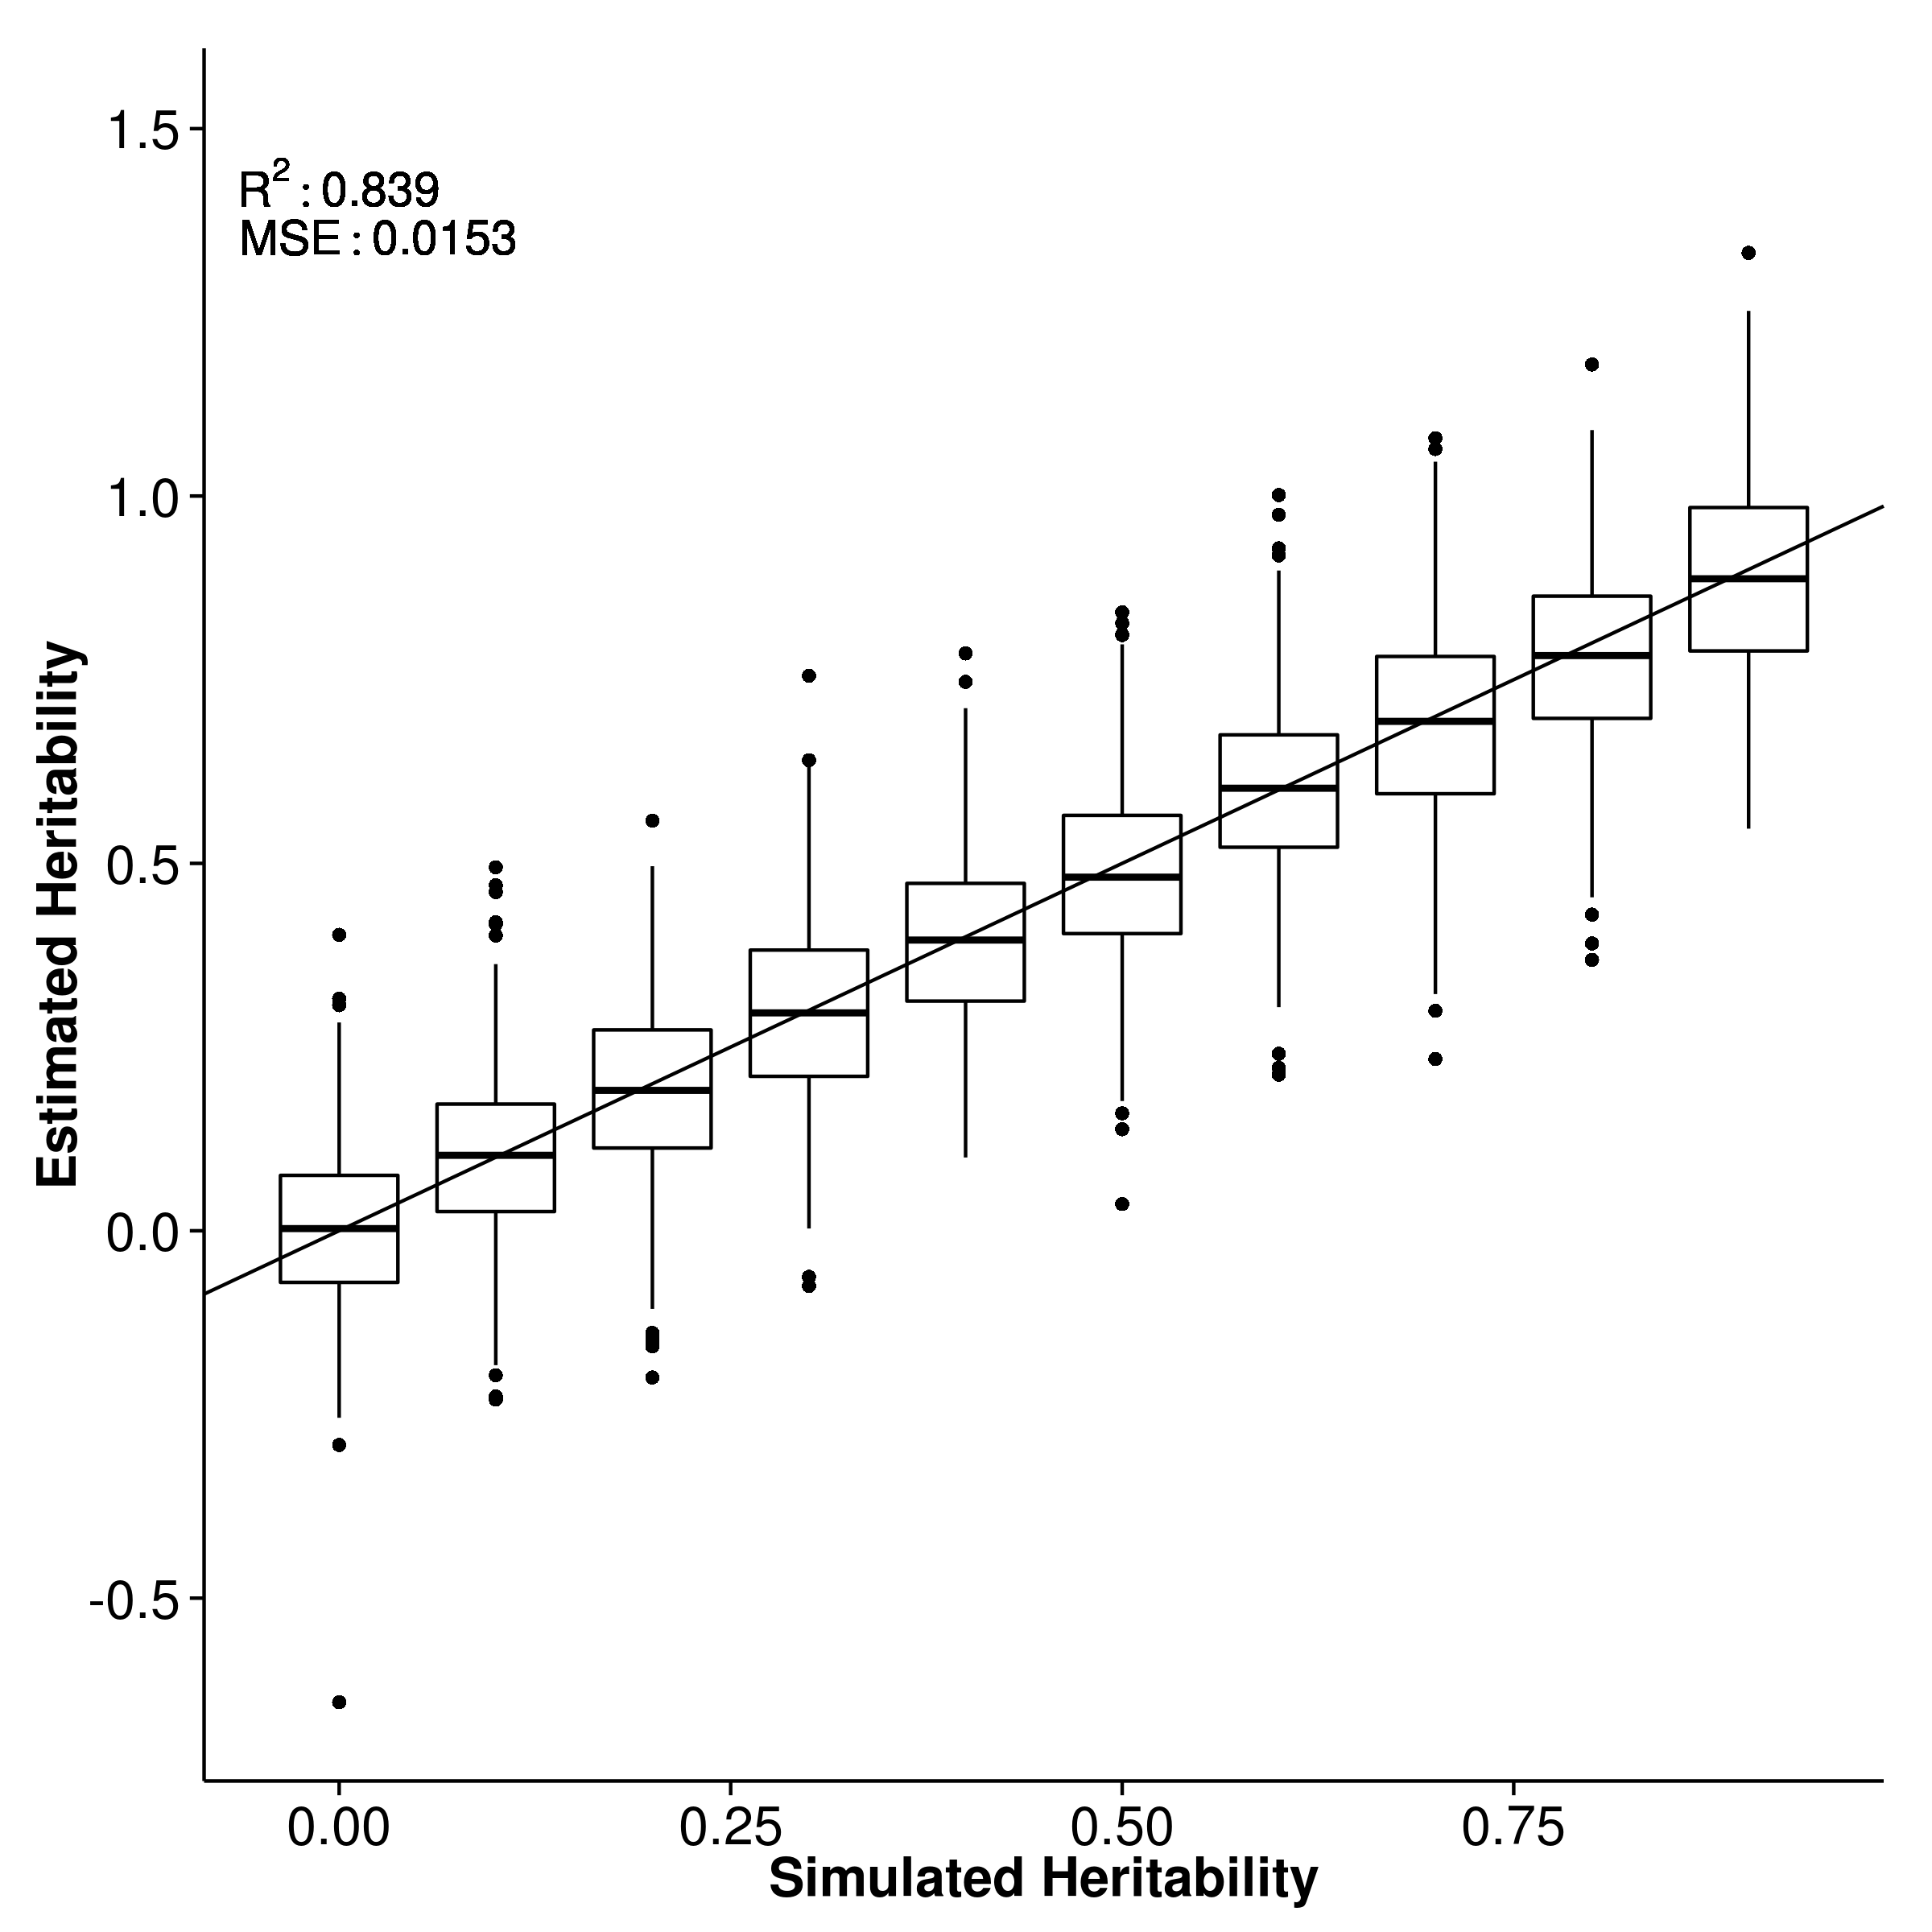
\includegraphics{figure/quantitative/random_effect/50c/shrek_50k_50c_meanH.png}}
				\label{fig:50k50cQtmeanSre}
			}
			\subfloat[GCTA]{
				\scalebox{.4}{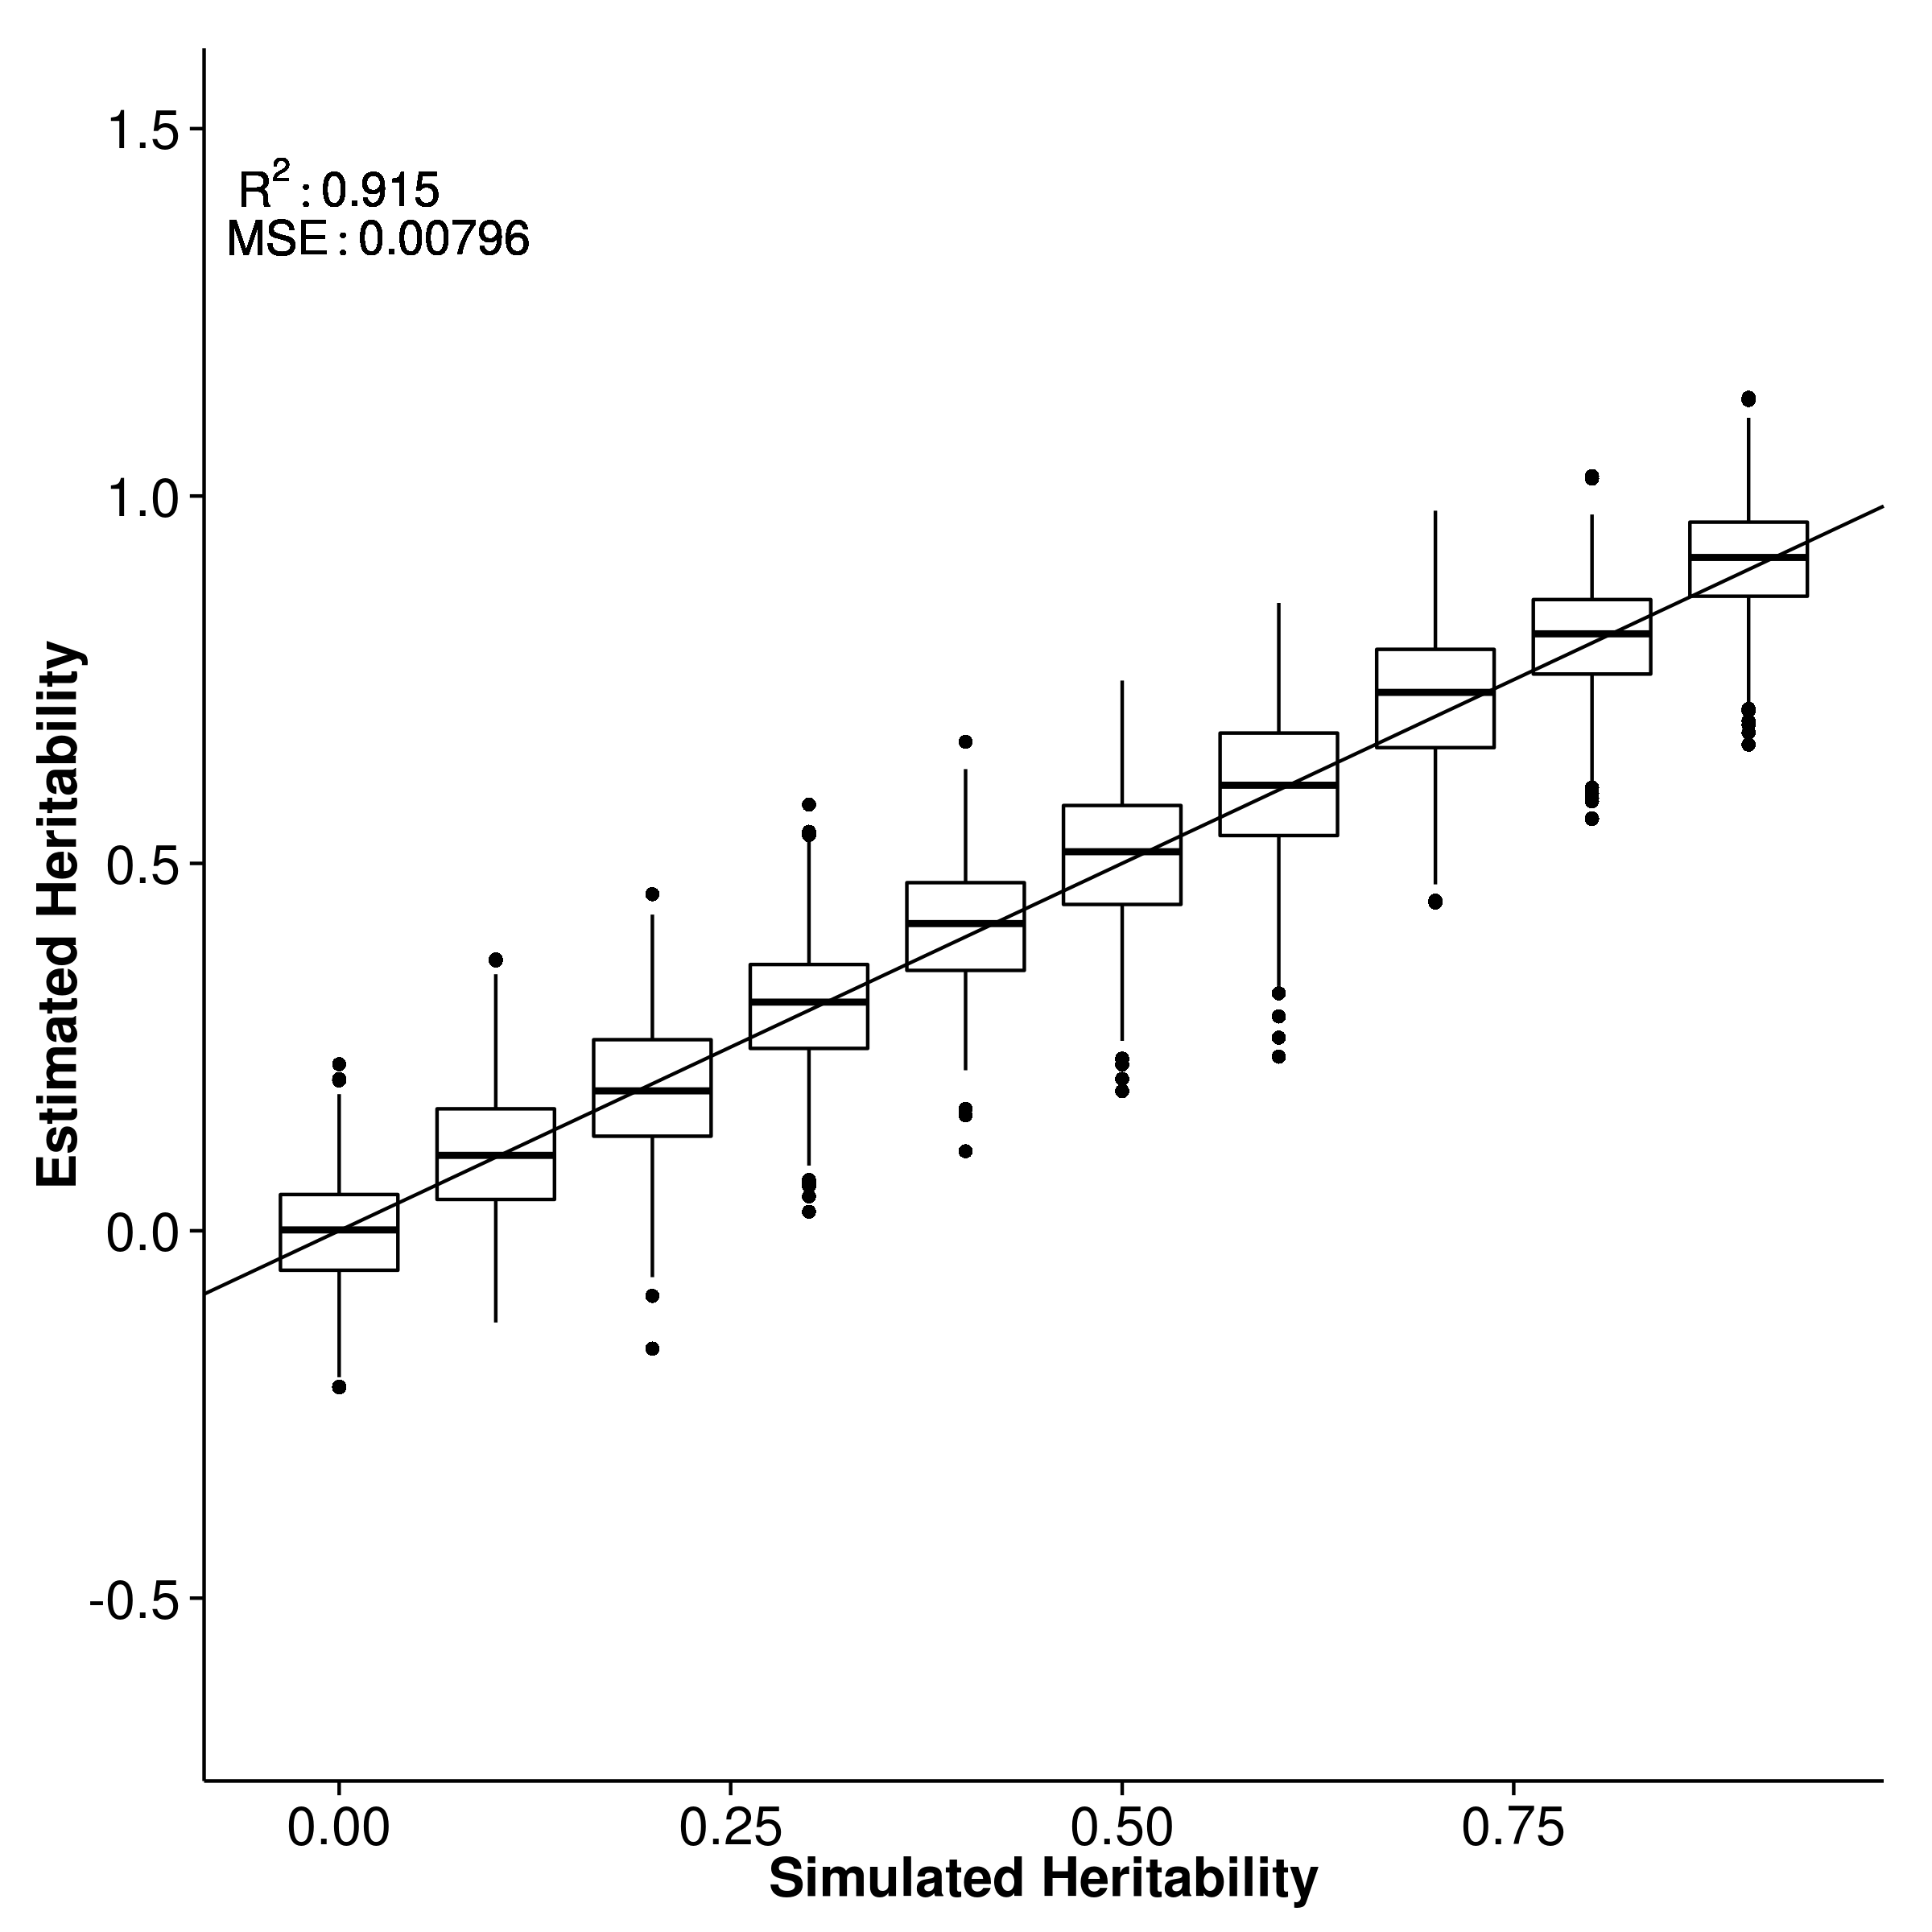
\includegraphics{figure/quantitative/random_effect/50c/gcta_50k_50c_meanH.png}}
				\label{fig:50k50cQtmeanGre}
			}\\
			\subfloat[LDSC with fix intercept]{
				\scalebox{.4}{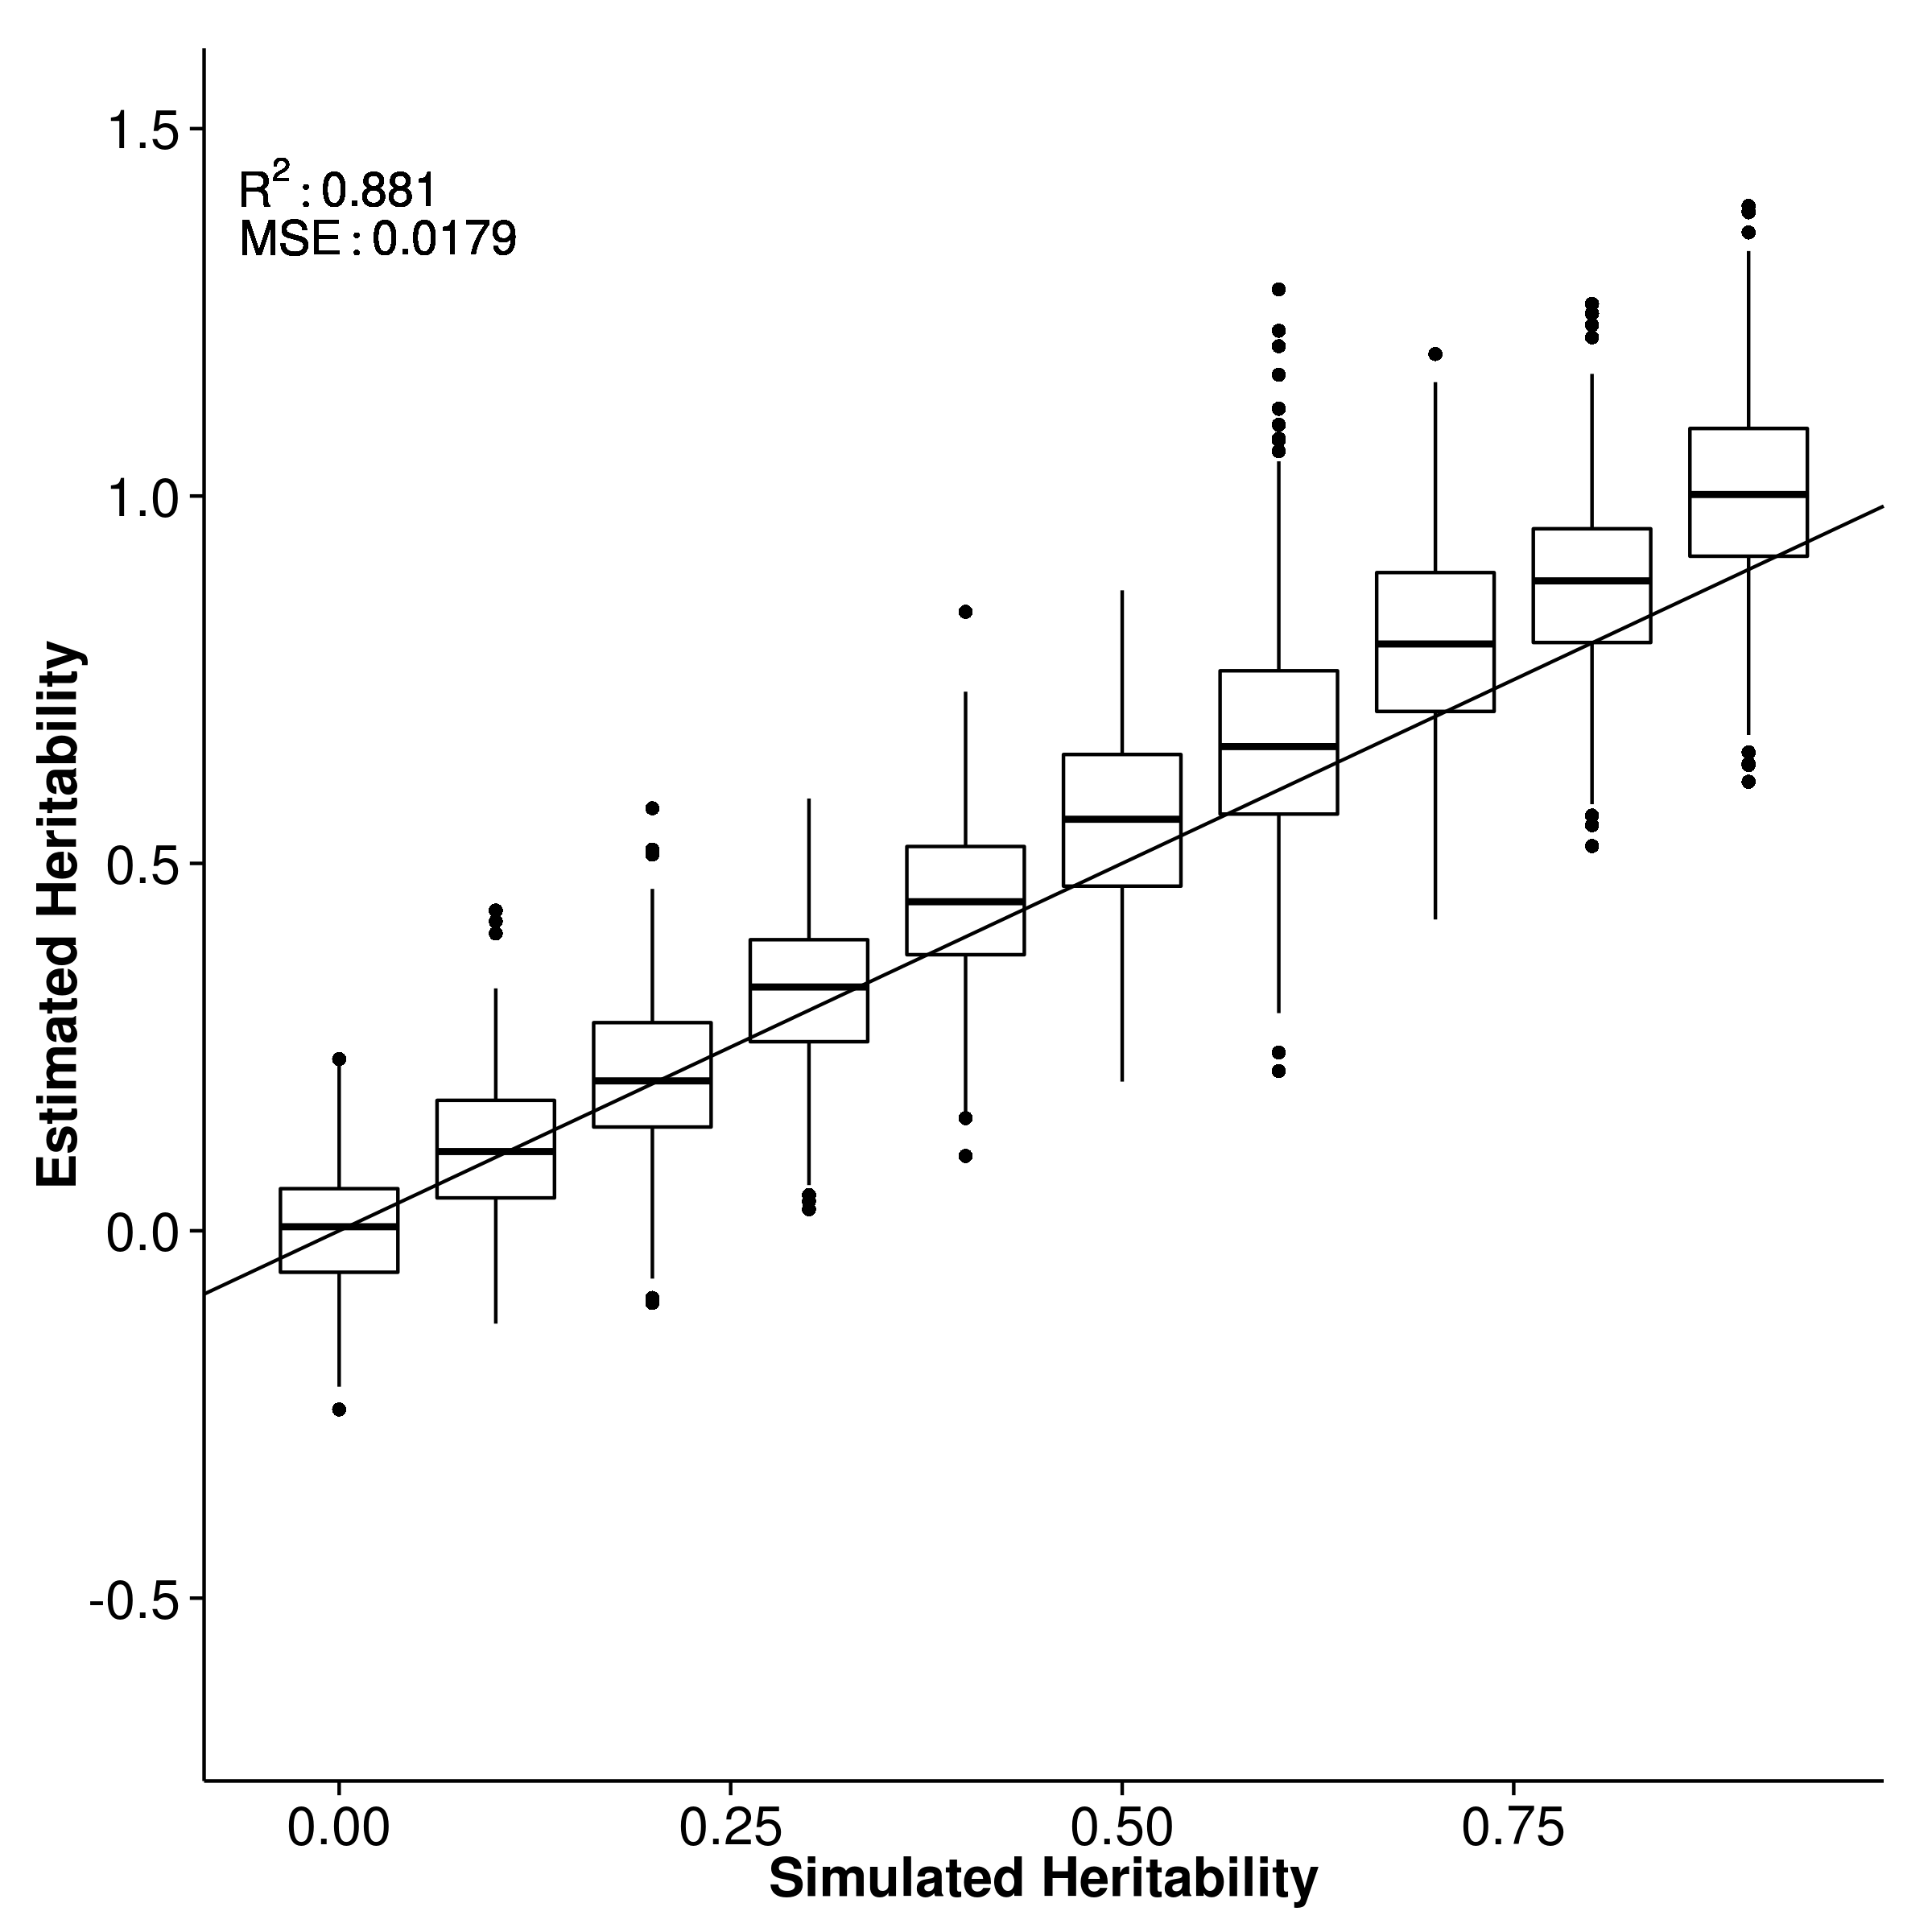
\includegraphics{figure/quantitative/random_effect/50c/ldsc_50k_50c_meanH.png}}
				\label{fig:50k50cQtmeanLre}
			}
			\subfloat[LDSC with intercept estimation]{
				\scalebox{.4}{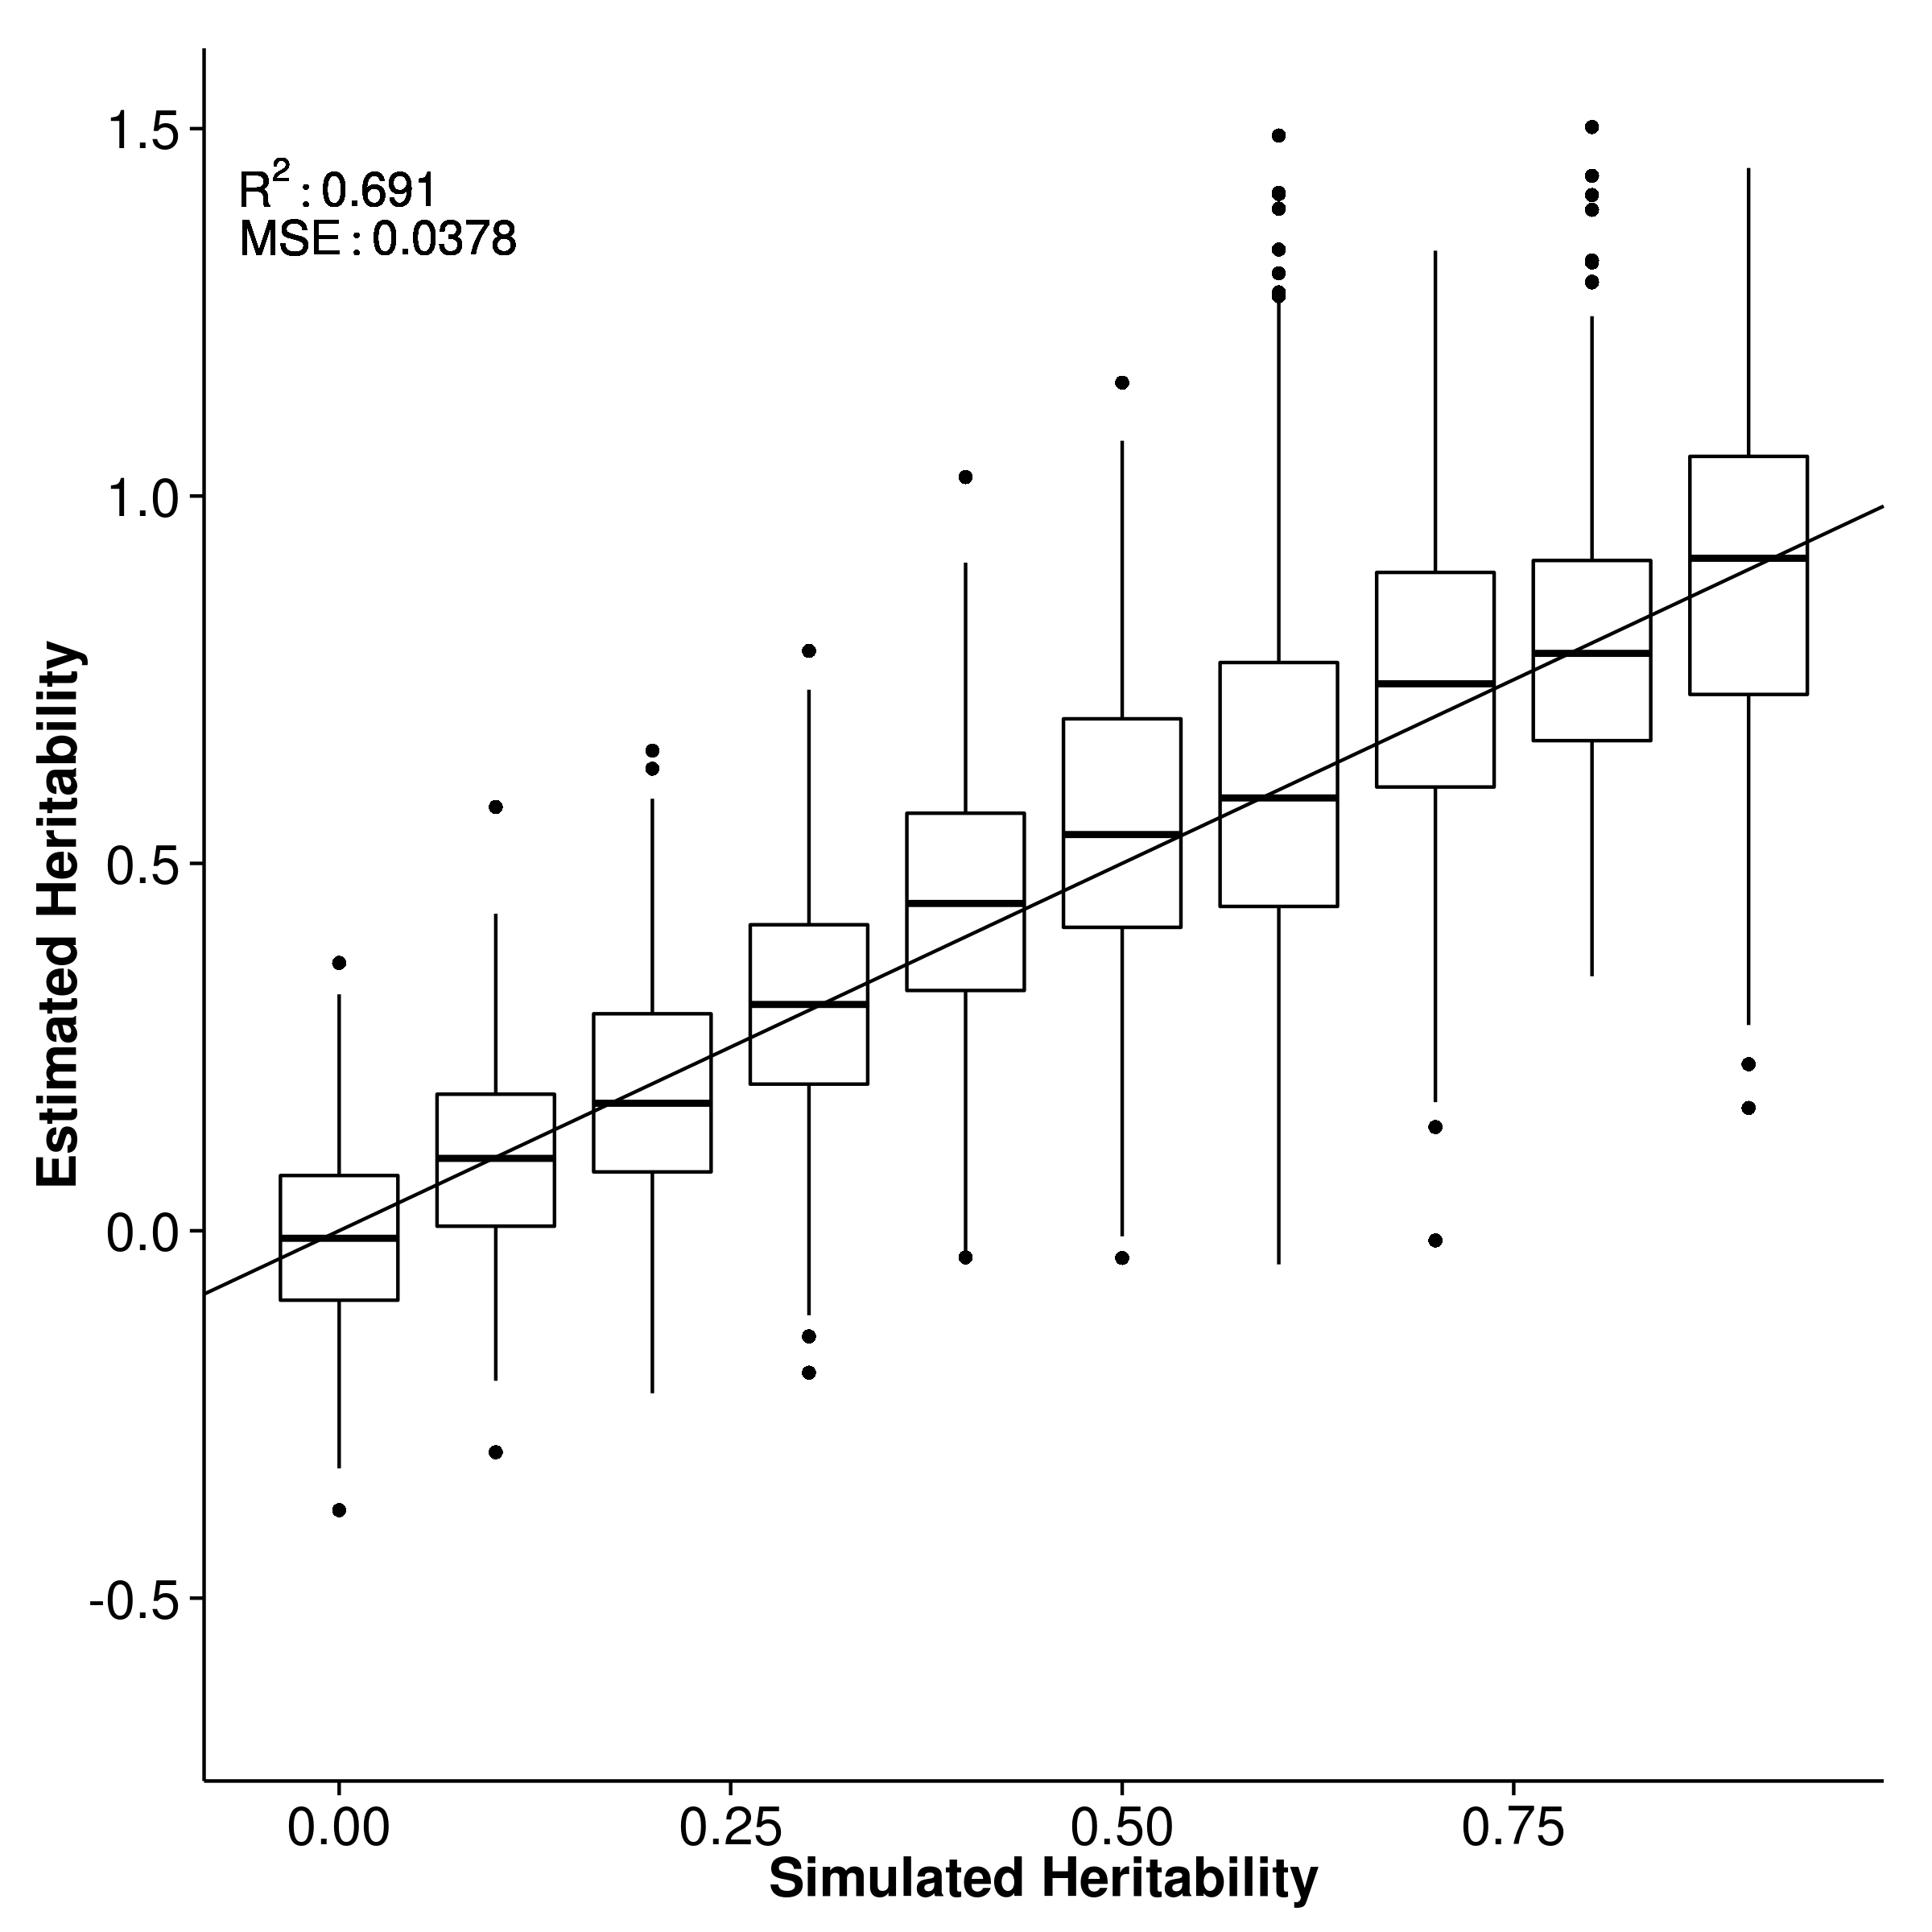
\includegraphics{figure/quantitative/random_effect/50c/ldscIn_50k_50c_meanH.png}}
				\label{fig:50k50cQtmeanIre}
			}
			\caption[Simulation of Quantitative Traits with 50k \glsentryshortpl{SNP} and 50 causal variants of random effect size]
			{Simulation of Quantitative Traits with 50k \glsentryshortpl{SNP} and 50 causal variants with random effect size.} 
			\label{fig:50k50cQtMeanre}
		\end{figure}
		\begin{figure}
			\centering
			\centering
			\subfloat[SHREK]{
				\scalebox{.4}{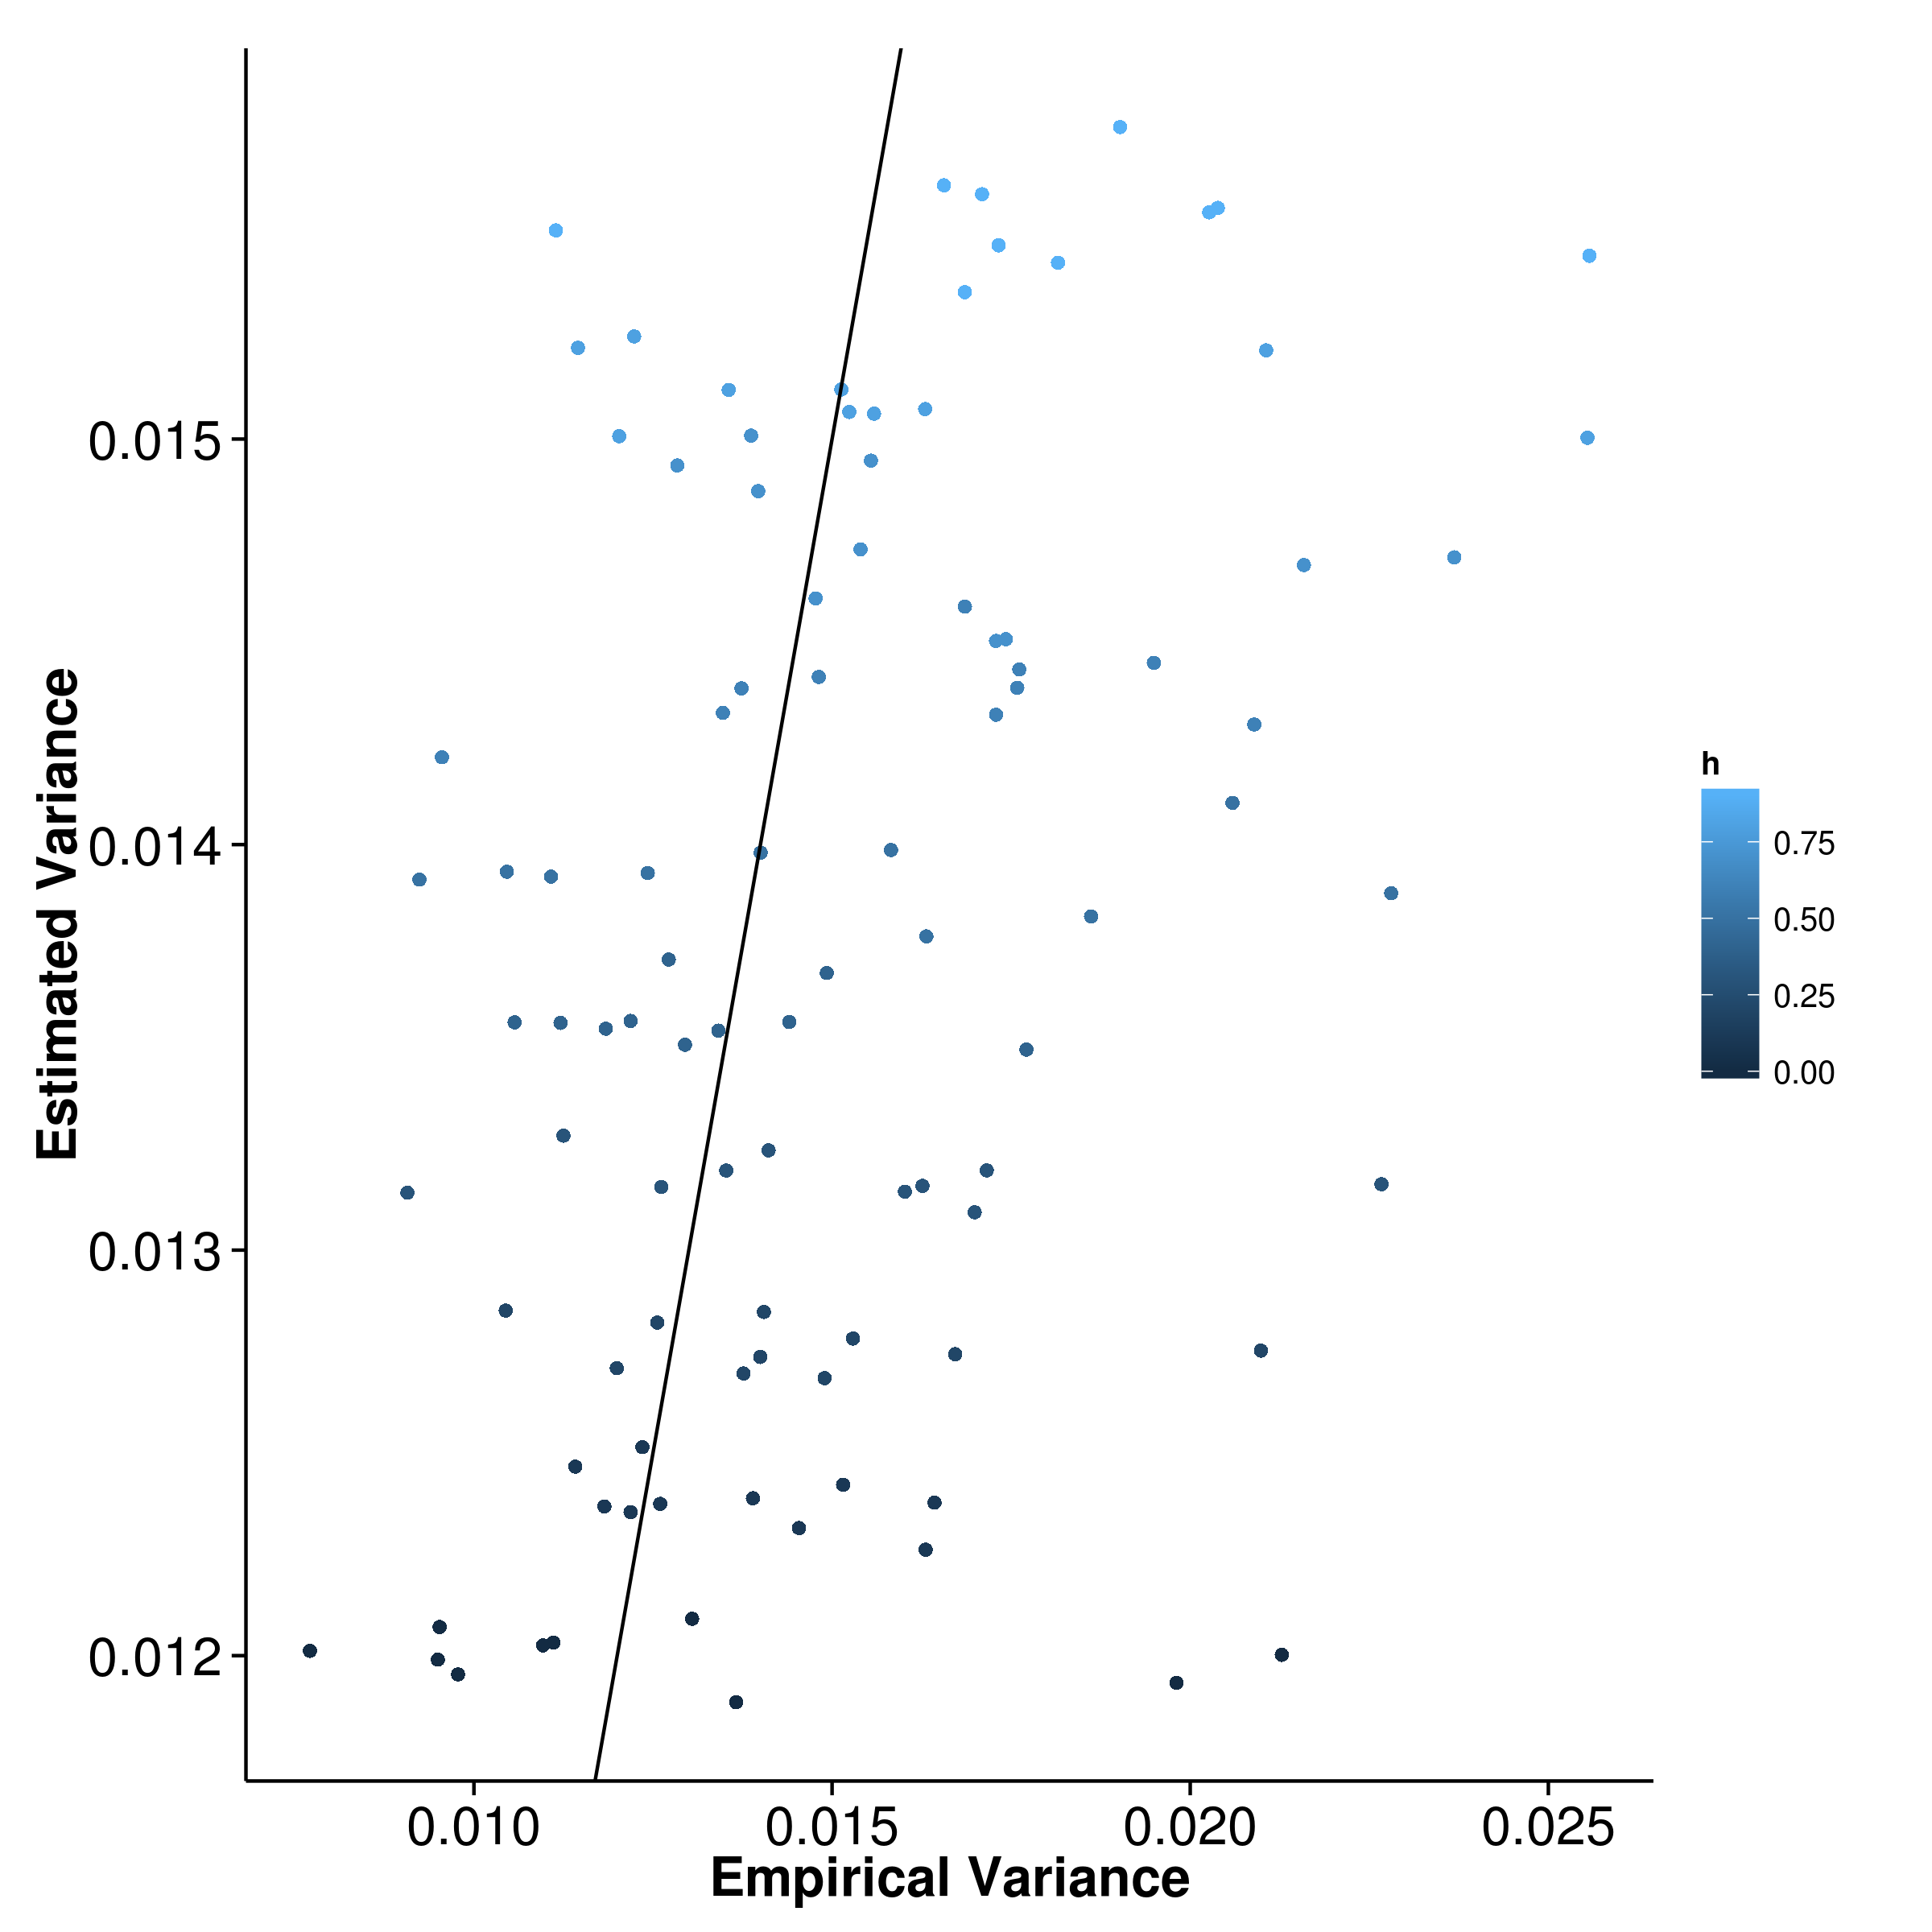
\includegraphics{figure/quantitative/random_effect/50c/shrek_50k_50c_varH.png}}
				\label{fig:50k50cQtvarSre}
			}
			\subfloat[GCTA]{
				\scalebox{.4}{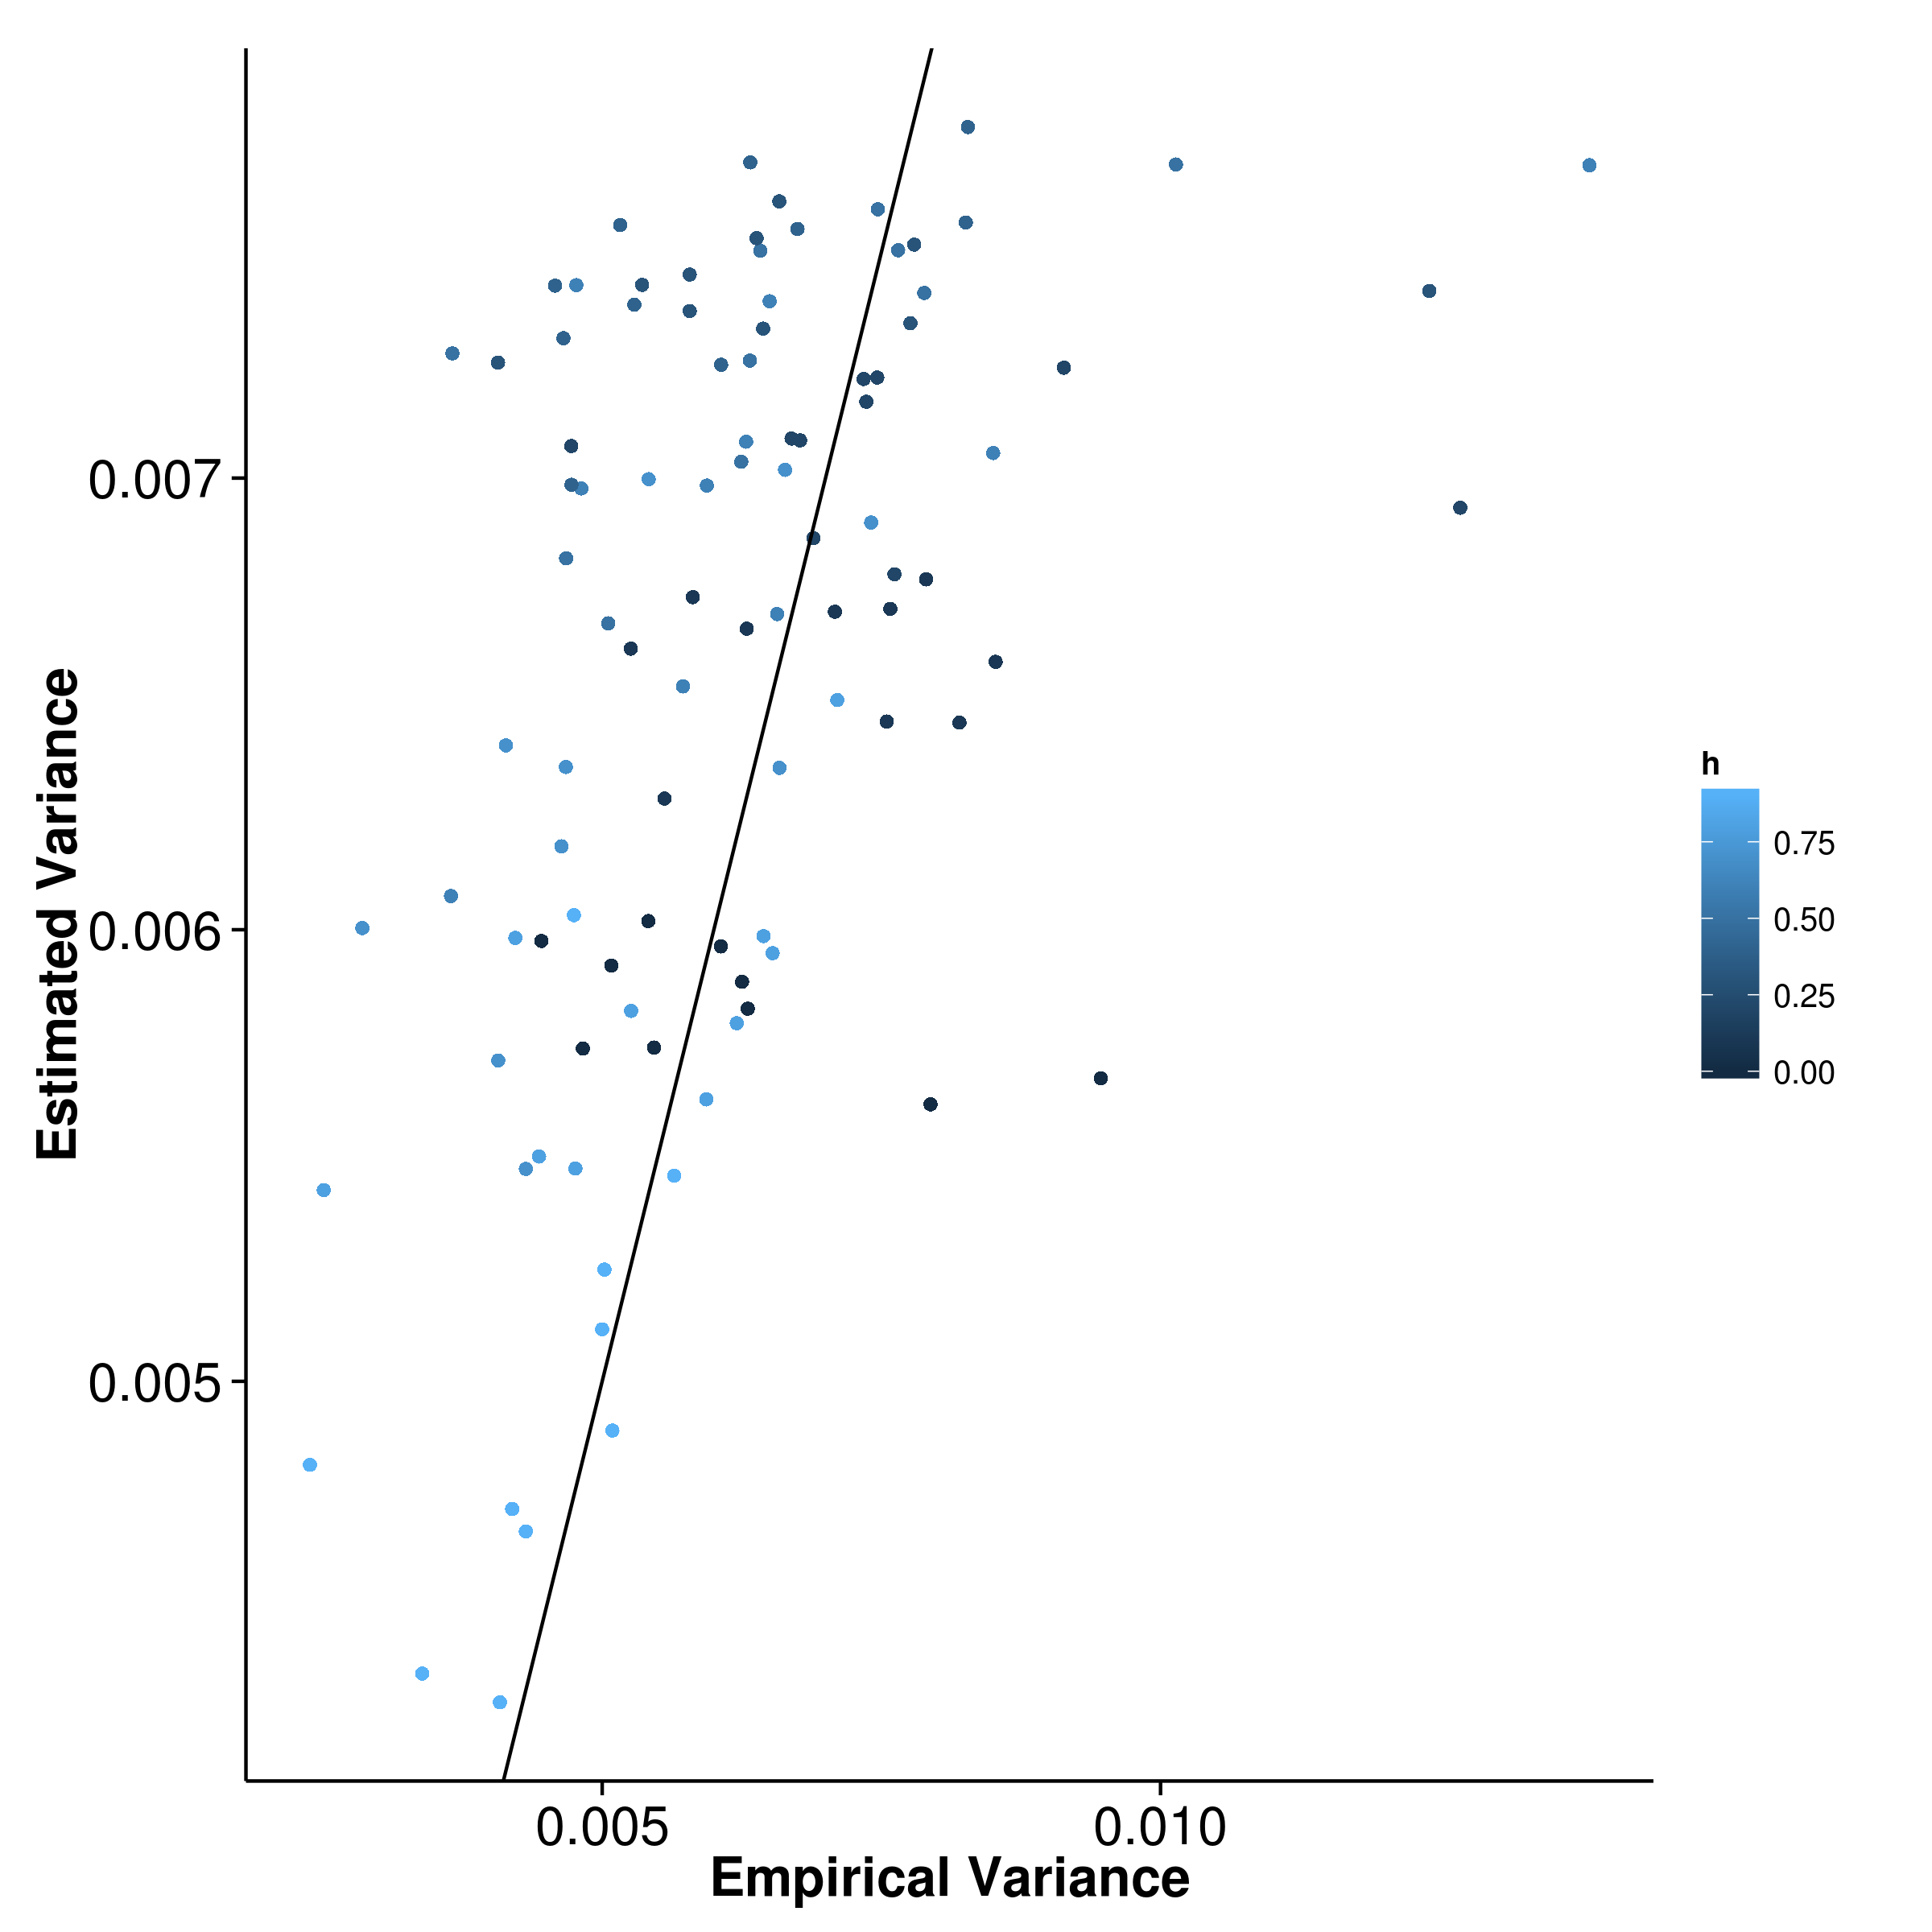
\includegraphics{figure/quantitative/random_effect/50c/gcta_50k_50c_varH.png}}
				\label{fig:50k50cQtvarGre}
			}\\
			\subfloat[LDSC with fix intercept]{
				\scalebox{.4}{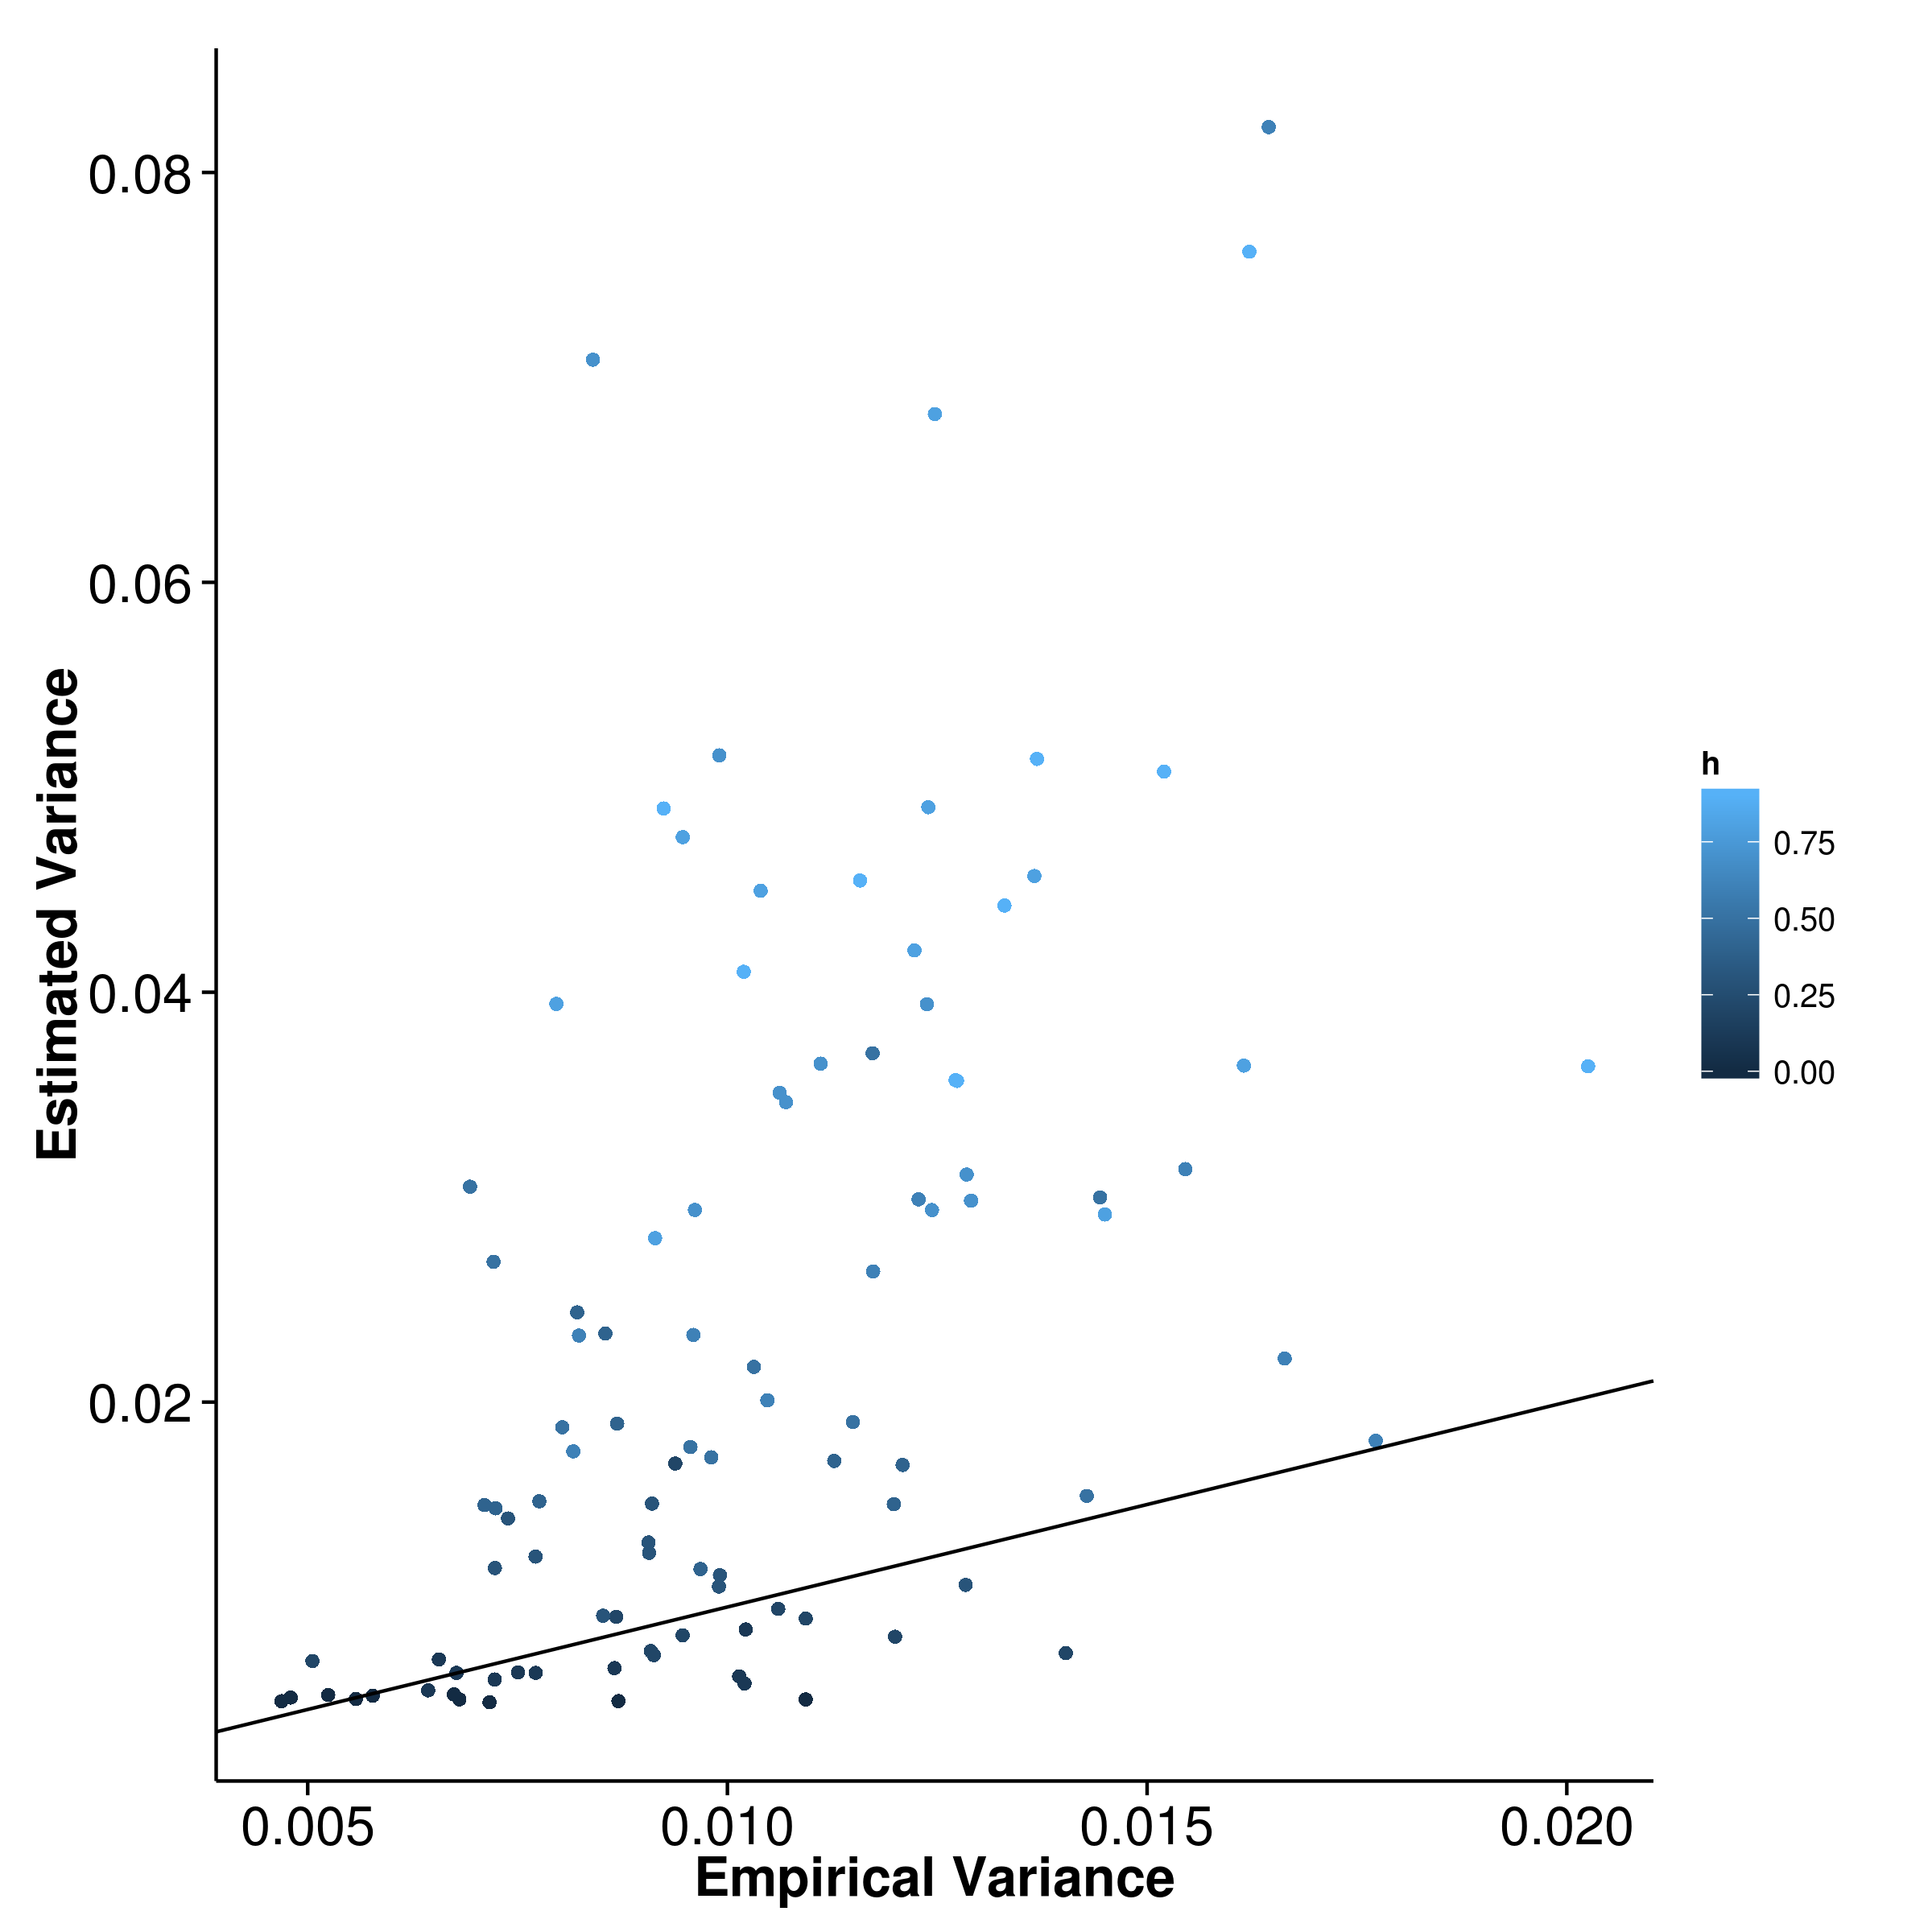
\includegraphics{figure/quantitative/random_effect/50c/ldsc_50k_50c_varH.png}}
				\label{fig:50k50cQtvarLre}
			}
			\subfloat[LDSC with intercept estimation]{
				\scalebox{.4}{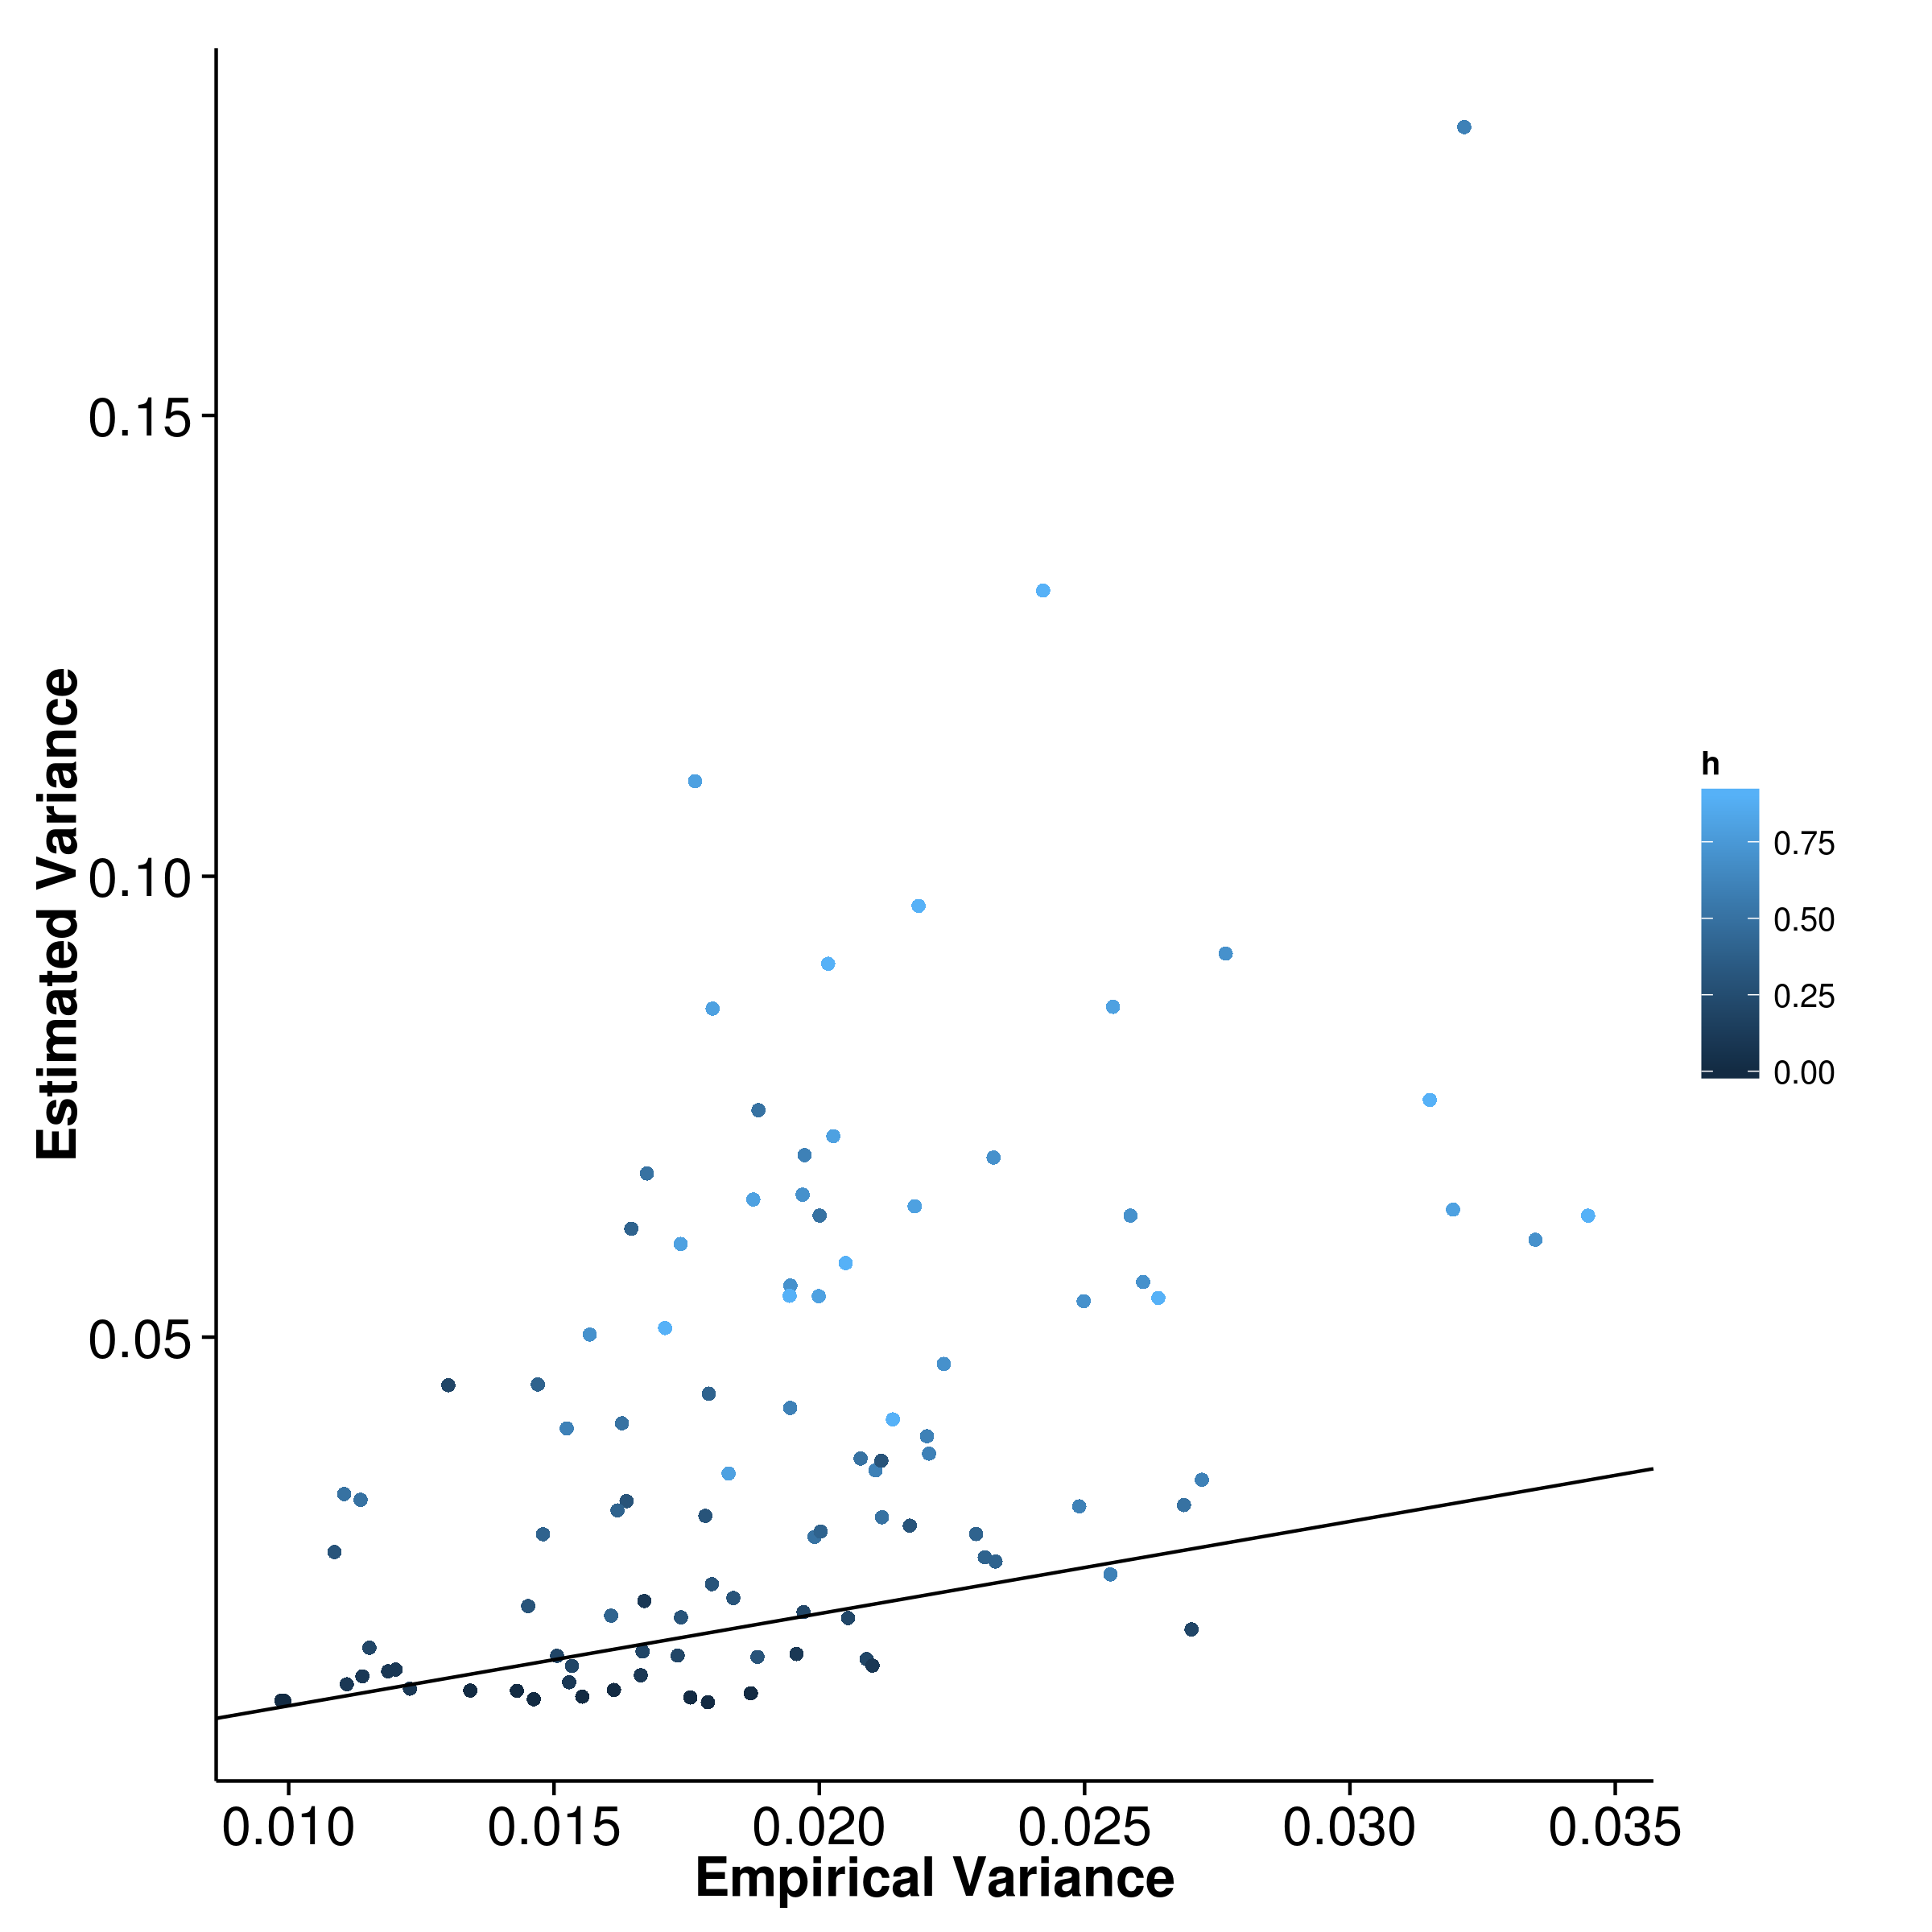
\includegraphics{figure/quantitative/random_effect/50c/ldscIn_50k_50c_varH.png}}
				\label{fig:50k50cQtvarIre}
			}
			\label{fig:50k50cQtVarre}
		\end{figure}
		
		
	\section{Discussion}